\chapter{Monolithic Pixel Detectors for HEP Applications}

%Monolithic silicon pixel detectors were previously described in chapter \note{chapter ref} and their promising performances for potential upgrades of current experiments or the development of novel experiments was highlighted. Notably, in \note{chapter ref} were discussed the prospects of the installation of a new pre-shower detector for the FASER experiment using Silicon-based pixel detectors for the active part of the detector. 

At the University of Geneva, the development of silicon-based monolithic pixel detectors has been carried out since 2016. The design of the sensors also relied on the implementation of ultra fast and low noise electronics offered by the SG13G2 \SI{130}{\nano\meter} process \cite{IHP130nm} consisting in a \SI{130}{nm} SiGe BiCMOS HBT offered by Leibniz Institute of High-Performance Microelectronics (IHP). Over the course of the years, both the sensor and the electronics design were refined in order to better understand the intrinsic limits on the performances of such devices. The research was mostly focused on investigating the efficiency and timing performance of the designed prototypes with the scope of eventually developing a very fast, fully efficient, radiation hard and low power consumption sensor, as a good candidate for applications in future colliders. In parallel, profiting from the expertise acquired, a proposal for an upgraded version of the pre-shower station in the FASER experiment was initiated.

The work presented in this chapter will first give a description of the design characteristics of two prototypes, a first one designed under the ATTRACT Phase1 MonPicoAD project, also referred to as the \textit{ATTRACT} prototype and a second one designed under the MONOLITH ERC Advanced project, also referred to as the \textit{MONOLITH} prototype. The discussion will remain at surface level as the scope of this thesis was neither the design of the sensor nor the design of the electronics but rather the testing and extensive comprehension of the features exhibited by each prototype.

One of the key figures of merit of the designed sensors is their time resolution. This performance metric is affected by many sources, some of which can eventually be corrected for. In the second part of the discussion, an overview of the different contributions to the time resolution of silicon-based sensors will be presented together their sources and also possible solutions to reduce their impact. 

The characterisation of such prototypes is essential and a robust and reliable testing procedure is required. Usually, such studies are performed using a particle beam composed essentially of minimum ionising particles. In the context of this research, prototypes were tested at the CERN SPS testbeam facility. The time resolution and detection efficiency was extracted for each prototype using a dedicated experimental setup. A reconstruction of the particle tracks onto the sensors was essential to perform position sensitive measurements. 
The last part of the discussion in this chapter will present first present the results of the characterisation of the \textit{ATTRACT} prototype, \note{also introducing routine for track reconstruction and data set contruction}  and secondly the results of the characterisation of the \textit{MONOLITH} prototype. Additionally, the effect of radiation on the performance obtained with the \textit{MONOLITH} prototype will also be presented for a wide range of radiation levels, up to values compatibles with the innermost layers of large experiments at CERN in the HL-LHC phase.    


%The last part of the discussion in this chapter will, in a first time cover the arguments mentioned above, and in a second time present the results of the characterisation of the \textit{ATTRACT} and \textit{MONOLITH} prototypes. Additionally, the effect of radiation on the performance obtained with the \textit{MONOLITH} prototype will also be presented for a wide range of radiation levels, up to values compatibles with the innermost layers of large experiments at CERN in the HL-LHC phase.    

	\clearpage
	\section{Prototypes and Design Characteristics}
	In the following section, the design characteristics of the sensor and electronic parts of the two prototypes tested in this work will be presented. The first prototype will be referred to as the \textit{ATTRACT} prototype while the second one will be referred to as the \textit{MONOLITH} prototype. Some key dates together with a list of the associated literature associated to each prototype are listed below: 
	\begin{itemize}
		\item \textbf{\textit{ATTRACT}} prototype (2019): 
		\begin{itemize}
			\item Tested in laboratory in 2020-21 and at testbeam facility in 2021, results published in: \textit{"Efficiency and time resolution of monolithic silicon pixel detectors in SiGe BiCMOS technology"} by G. Iacobucci et al. in JINST in 2022 \cite{ATTRACT_proto1_50ps}. 
		\end{itemize}
		\item \textbf{\textit{MONOLITH}} prototype (2022):
		\begin{itemize}
			\item Tested in the laboratory and at testbeam facility in 2022, results published in: \textit{"20 ps time resolution with a fully-efficient monolithic silicon pixel detector without internal gain layer"} by S. Zambito et al. in JINST in 2023 \cite{MONOLITH_proto2_20ps}.
			\item Tested after irradiation in the laboratory in 2023, results published in \textit{"Radiation Tolerance of SiGe BiCMOS Monolithic Silicon Pixel Detectors without Internal Gain Layer"} by M. Milanesio et al. in JINST in 2023 \cite{MONOLITH_RadHard_lab}.
			\item Tested at testbeam facility in 2023, results published in : \textit{"Testbeam results of irradiated SiGe BiCMOS monolithic pixel detector without internal gain layer"} by T. Moretti et al. in JINST in 2024 \cite{MONOLITH_RadHard_testbeam}.
		\end{itemize} 
	\end{itemize}

		\subsection{ATTRACT Prototype}
		The \textit{ATTRACT} prototype (2019) is the second prototype designed the scope of the ATTRACT Phase1 MonPicoAD project. Its predecessor was described and tested in \cite{ATTRACT_proto1, ATTRACT_proto1_50ps}. The ASIC was manufactured by the IHP Microelectronics foundry using the IHP SG13G2 \SI{130}{\nano\meter} BiCMOS technology. The design of the ASIC was finalised in 2019 and the wafers received after post processing in 2019. The ASIC has a total size of $2.3 \times 2.5$ mm$^2$ active pixel matrix is subdivided in 12 rows and columns for a total of 144 hexagonal pixels with a \SI{65}{\micro\meter} side resulting in a pixel pitch of roughly \SI{110}{\micro\meter}. The ASIC periphery is located beside the pixel matrix and includes a Slow-Control (SC) interface through which the different bias supplied to the electronics can be controlled. The periphery and pixel matrix is then insulated from the substrate by a total of 18 guard rings which insulates the pixel well from the substrate. The pixel matrix is further subdivided into four 6x6 matrices, each containing a different design for the preamplifier part of the frontend electronics.  
			
		Within one of the four sub-matrices, a set of four pixels are connected to a SiGe HBT amplifier, used as a charge sensitive amplifier, and analog driver directly connect to the output pads. The driver itself is composed of two consecutive HBTs in common collector configuration with a first AC stage coupled to the output of the amplifier \cite{ATTRACT_proto1_testbeam}. The frontends are located outside of the pixel well and are used to measure and amplify the charge deposited by particles in the sensor. In the results later presented in \note{insert section}, the performances quoted are referred to these four analog pixels. The remaining 140 pixels have their frontend located in pixel and are connected to a digital readout with many discrimination stages, different from one sub-matrix to the other. These pixels also have the output of their discriminator connected to a FAST-OR to provide a discriminated signal for all of them in output. 
		
		The active part of the ASIC is build as a \textit{n-on-p} sensor meaning that the pixel well is n-type and the substrate is p-type. The base substrate is doped with Boron and a resistivity of \SI{50}{\ohm \centi\meter}. After implementation, the substrate was thinned to reach a sensor thickness of roughly \SI{60}{\micro\meter}. The total pixel capacitance in input to the preamplifier is estimated to be \SI{80}{\femto\farad} with a depletion depth estimated to be \SI{23}{\micro\meter}. 
		
		An image of the prototype taken under a microscope with overlayed blocks representing the diverse sections of the ASIC is presented in figure \ref{im:ATTRACT_ASIC_layout}.
		\begin{figure}[h]
			\centering
			\includegraphics[width=0.65\linewidth]{files/ATTRACT_ASIC_layout}
			\caption{Image of the \textit{ATTRACT} prototype taken with a microscope. On top of the image are placed different block representing the different key structure in the ASIC. \note{Add zoom on pixel matrix and add analog frontend label and names of pixels}}
			\label{im:ATTRACT_ASIC_layout}
		\end{figure} 
		
		
		
		
		\subsection{MONOLITH Prototype}
		
		The \textit{MONOLITH} prototype (2022) is the second prototype of the generation of sensors without internal gain layer designed in the scope of the MONOLITH project. The ASIC was manufactured by the IHP Microelectronics foundry using the IHP SG13G2 \SI{130}{\nano\meter} BiCMOS technology. The design of the ASIC was finalised in 2021 and the wafers received after post processing in 2022. The ASIC has a (smaller) total size of $2.0 \times 2.5$ mm$^2$ active pixel matrix is subdivided in the same was as the \textit{ATTRACT} prototype. The architecture of this prototype is mostly similar to the one presented for the \textit{ATTRACT} prototype except for a few changes.  
		
		The frontend design in this prototype is different than the one implemented in the \textit{ATTRACT} prototype as it includes improvements. The first noticeable difference is in the power distribution, indeed the previously the alimentation of the preamplifier and the driver were put together but are now separated. This design change has the objective of removing undesired cross-talk between the four analog pixels. The second modification affects the stability of the front end when operated in high gain configurations. This was achieved by equipping the driver stage with a semi-differential analog output, effectively reducing the common-mode noise outside the ASIC. In addition, the new driver design reduced the signal rise-time, a key parameter in the contribution to the time resolution. Finally, in contrast to the single-ended output used previously, this prototype provides a differential output, helping by offering means to reduce the external noise contributions when analysing the signals offline. 
		
		For what regards the sensor, the ASIC is build as a \textit{n-on-p} sensor meaning that the pixel well is n-type and the substrate is p-type. The base substrate is doped with Boron and is characterised by its very low resistivity of \SI{0.1}{\ohm \centi\meter} while the \SI{50}{\micro\meter} thick epitaxial layer grown on top is still doped with Boron but with a higher resistivity of \SI{350}{\ohm \centi\meter}. This value is to be compared with the \SI{50}{\ohm \centi\meter} of the previous prototype, leading to a larger production of initial charge in the sensor when crossed by a ionising particle. The total pixel capacitance in input to the preamplifier is estimated to be \SI{100}{\femto\farad}. 
		
		An image of the prototype taken under a microscope with overlayed blocks representing the diverse sections of the ASIC is presented in figure \ref{im:MONOLITH_ASIC_layout}.
		\begin{figure}[h]
			\centering
			\includegraphics[width=0.65\linewidth]{files/MONOLITH_ASIC_layout}
			\caption{Image of the \textit{MONOLITH} prototype taken with a microscope. On top of the image are placed different block representing the different key structure in the ASIC. \note{Add zoom on pixel matrix and add analog frontend label and names of pixels}}
			\label{im:MONOLITH_ASIC_layout}
		\end{figure} 
		 
		
		
	\clearpage
	\section{Time Resolution of Silicon Pixel Detectors}
	One of the main focuses of the development of silicon-based monolithic pixel detectors, first under the ATTRACT project and then under the MONOLITH project, is the achievement of very good time resolution, trying to get as close as possible to the intrinsic limits of the technologies implemented. The time resolution is defined as the error one makes when measuring the time of passage of a particle in the active part. There are multiple contributions to the time resolution of a silicon-based device, both from the sensor itself, the frontend electronics and the digital readout. The contribution from the digital readout for the studies carried out in this work is the one of the oscilloscope used to readout the 4 analog pixels as explained in \note{section ref}. 
	
	In order to better explain was time walk is, a collection of waveforms from the testbeam test of the \textit{MONOLITH} prototype was put together in figure \ref{im:waveforms_timeresolution}. There waveforms were aligned vertically with respect to each waveform's average level in the region before the signal but also horizontally using a very precise timing reference. The close-up view shows the time at which each waveforms would cross a discrimination threshold labeled $V_{th}$, also known at Time of Arrival ($ToA$) of the signal.
	\begin{figure}[h]
		\centering
		\includegraphics[width=0.85\linewidth]{files/waveforms_timeresolution}
		\caption{Collection fo waveforms from the \textit{MONOLITH} prototype in a testbeam with 120 GeV/c pions at CERN. The image shows time and amplitude aligned waveforms for a large range of amplitudes. The zoomed-in figure shows the time at which each waveform would cross a fixed voltage threshold ($V_{th}$), highlighting the spread of the time of arrival.}
		\label{im:waveforms_timeresolution}
	\end{figure} 
	
	If one was to build a distribution of the $ToA$, the shape of the distribution obtained is close to the one of a Gaussian function. The standard deviation of the fit of the ToA distribution with a Gaussian function gives the total time resolution of the system composed of the sensor, the frontend electronics and the readout system. 
	
	It is possible to group into four different categories the contributions to the time resolutions as listed by \cite{timeres_SiliconDetectors}:
	\begin{itemize}
		\item \textit{Signal creation}: The distribution of the energy deposited by the impinging particle depends on the physics of the interaction, some statistical fluctuations in the signal's induction can create irregularities in the signal, labeled $\sigma_{\text{Landau}}$. The variation on the amplitude of the signal due to smaller or larger charge deposition has a contribution too, labeled as $\sigma_{\text{time walk}}$. The first contribution is an intrinsic property of the detector defined by its geometry and operation. On the contrary, the time-walk can be correct as it will later be shown.
		\item \textit{Sensor characteristics}: The uniformity of the key components taking parts in the signal inducting such as the weighting field of drift velocities of the charge carriers can also lead to a distorsion of the signal, this contribution is labeled $\sigma_{\text{distorsion}}$.
		\item \textit{Electronics}: The noise of the amplifier is the key aspect here, its impact it more or less important depending also on the slew-rate of the amplifier, or how fast the signal can rise. This contribution is labeled $\sigma_{\text{jitter}}$
		\item \textit{Digitisation}: When the analog waveform is sampled for digitisation, the uncertainties on the measured time is associated to the TDC uncertainties and is labeled $\sigma_{\text{TDC}}$
	\end{itemize} 
	
	Each single contribution can be considered as independent from the others, assuming gaussian uncertainties, the total uncertainty of the time resolution $\sigma_t$ can be expressed as: 
	\begin{equation}
		\sigma_t^2 = \sigma_{\text{Landau}}^2 + \sigma_{\text{time walk}}^2 + \sigma_{\text{distorsion}}^2 + \sigma_{\text{jitter}}^2 + \sigma_{\text{TDC}}^2
	\end{equation}
	
	It is possible to discuss each contributions individually to better understand the origins of each contribution with the scope of understanding how the design of the full detector ca be optimised. 
	
	 	\subsection{Charge Collection Noise Contribution}
% TODO: CH4: Check that the description with Landau is correct, the total event is one point in a Landau so that the total amplitude is a Landau (see TB plots), but at the level of single events, it is more something like a struggling function, that is a deviation from the Landau. there are interactions at the level of the single shells on the atom. 

	 	The energy lost by a charged particle when traversing a material arises primarily from electromagnetic interactions, in which the transferred energy results in ionisation or excitation of the target medium. For relativistic particles with energies well above the electron mass, the average energy loss per unit length is material-dependent and is accurately described by the Bethe formula:

		\begin{equation}
			\left\langle -\frac{dE}{dx} \right\rangle = K z^2 \frac{Z}{A} \frac{1}{\beta^2} \left[ \frac{1}{2} \ln\left( \frac{2 m_e c^2 \beta^2 \gamma^2 W_{\text{max}}}{I^2} \right) - \beta^2 - \frac{\delta(\beta \gamma)}{2} \right],
		\end{equation}

		where $K$ is a constant, $z$ is the charge of the incident particle, $Z$ and $A$ are the atomic number and mass number of the medium, $\beta$ and $\gamma$ are the relativistic parameters, $I$ is the mean excitation potential of the material, and $W_{\text{max}}$ the maximum energy transferable in a single collision.

		To better illustrate the behaviour of energy loss across a wide range of particle velocities, figure \ref{im:bethe_bloch} shows the mass stopping power (i.e. the energy loss per unit length scaled by the density of the medium) in copper as a function of $\beta \gamma$, ranging from $10^{-3}$ to $10^5$ \cite{PDG}.

		\begin{figure}[h]
			\centering
			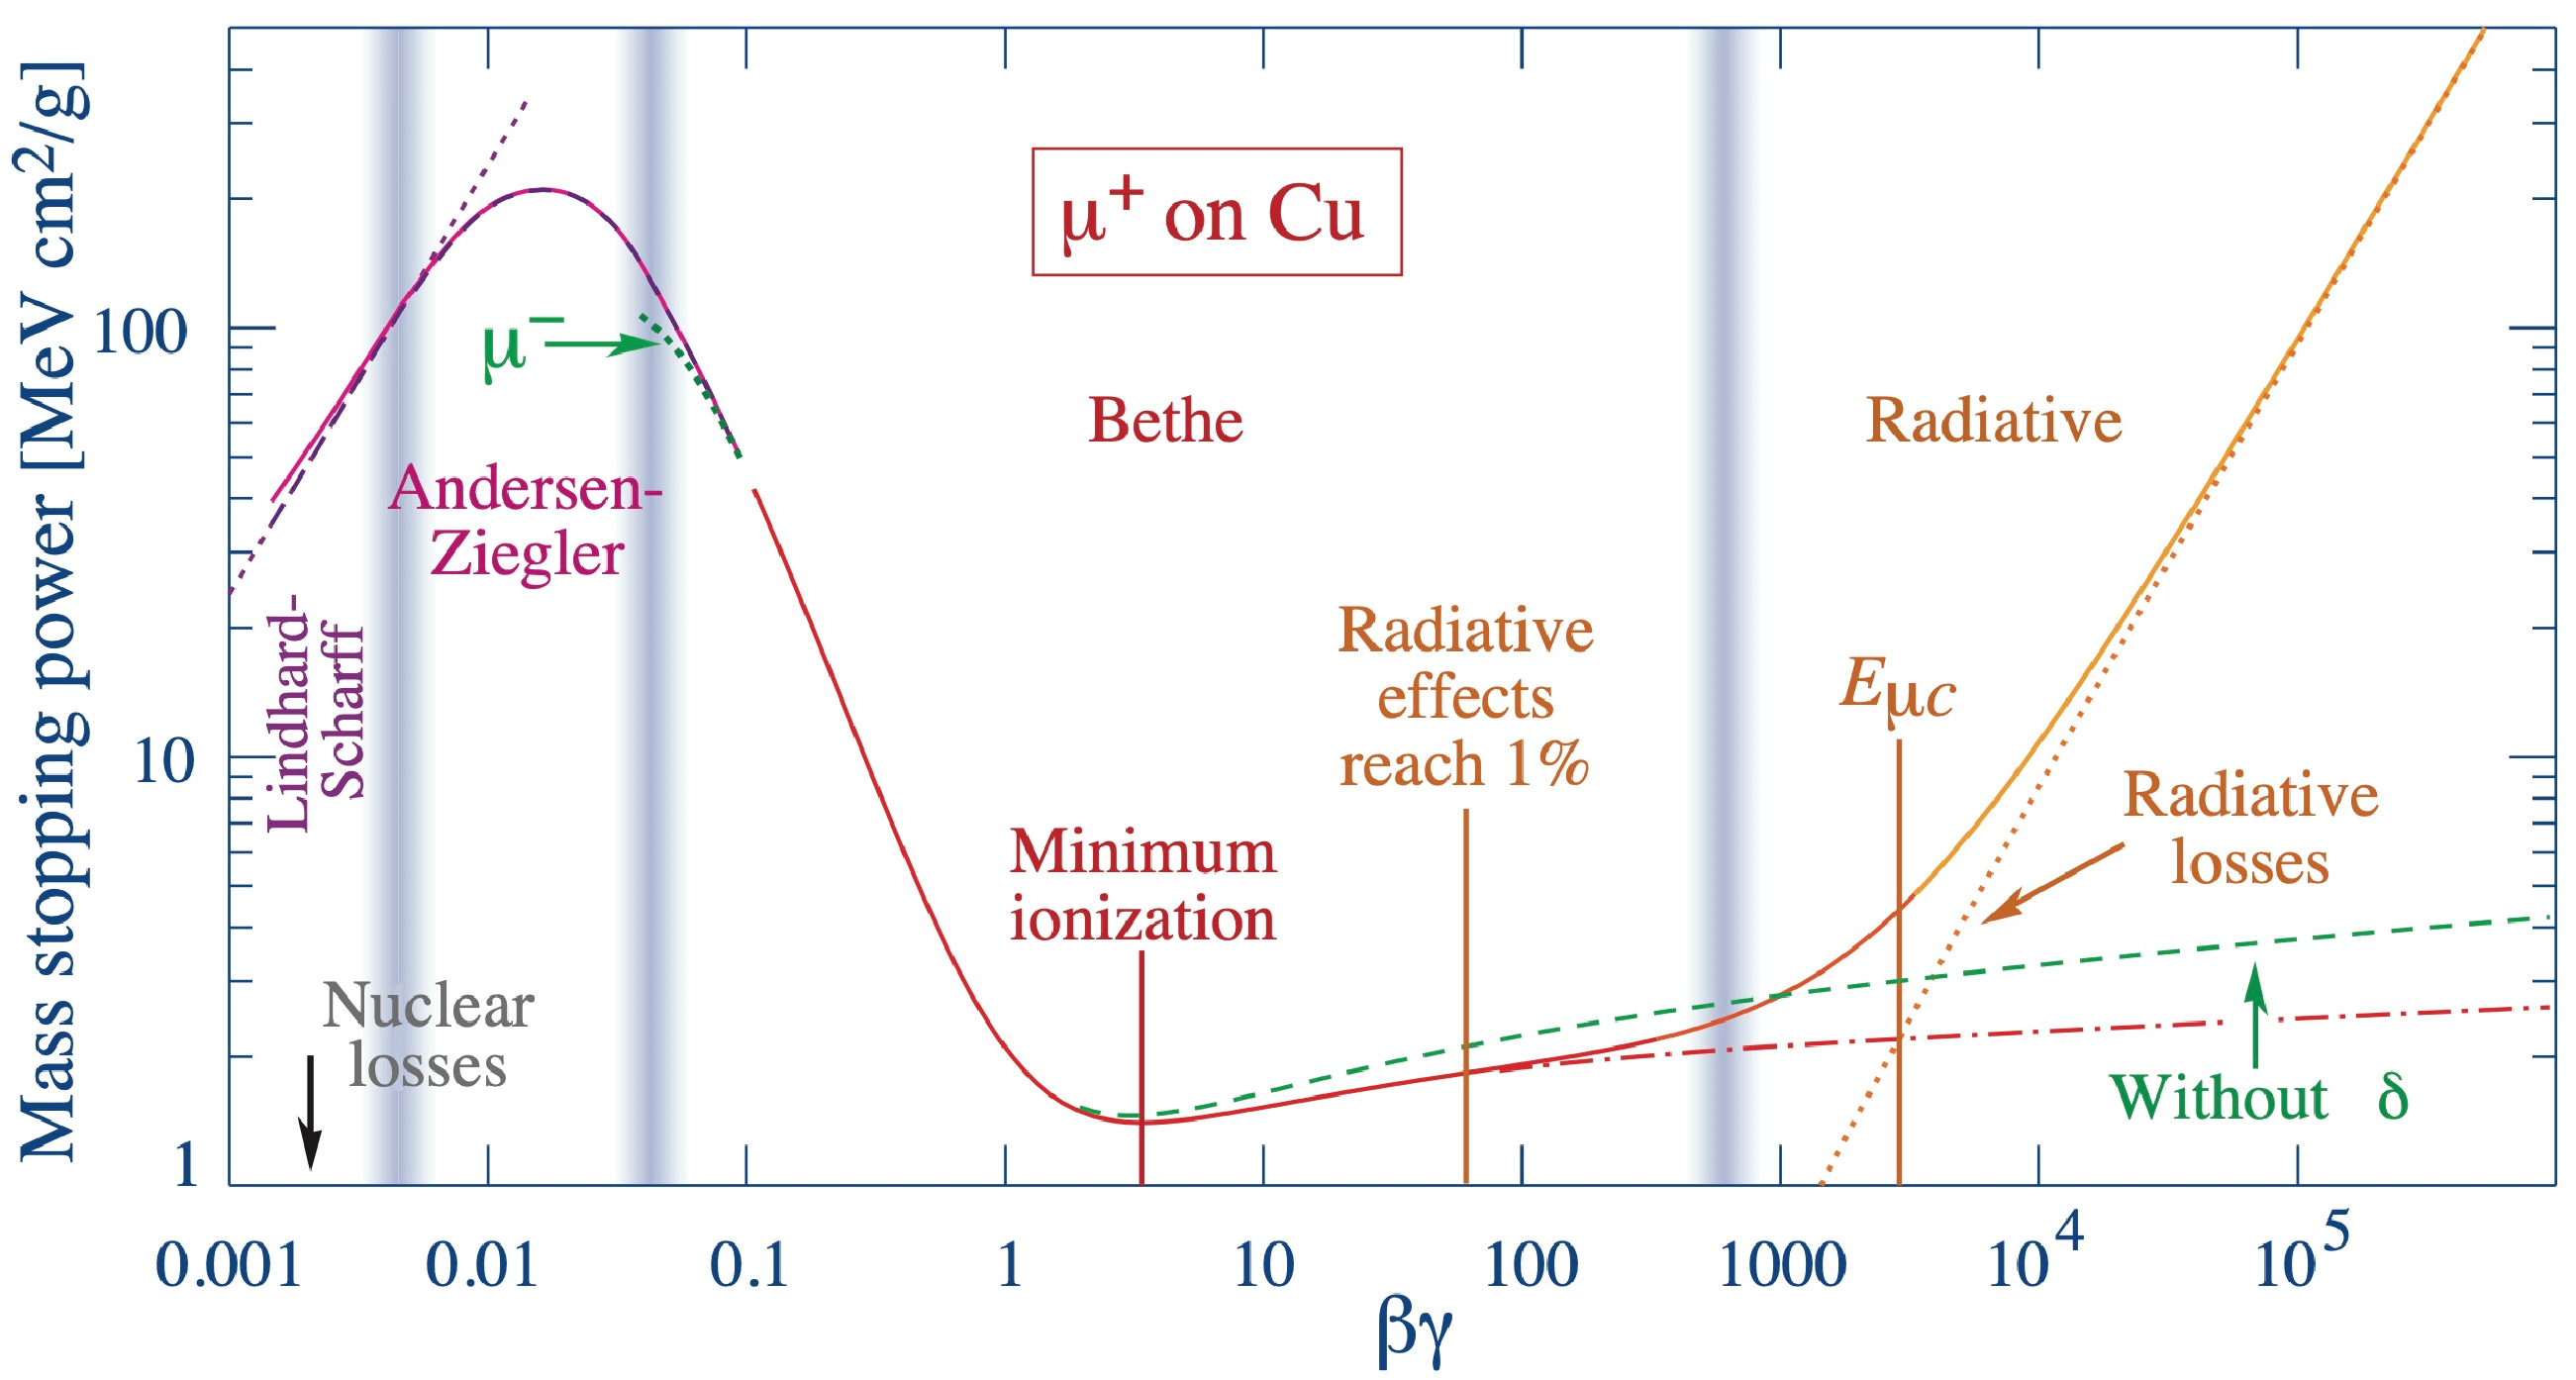
\includegraphics[width=0.85\linewidth]{files/bethe_bloch}
			\caption{Mass stopping power for charged particles with $\beta \gamma$ ranging from $10^{-3}$ to $10^5$ in copper.}
			\label{im:bethe_bloch}
		\end{figure}

		One of the key features is the minimum ionisation point, which occurs for particles with $\beta \gamma \simeq 3$. Such particles are referred to as Minimum Ionising Particles (MIPs) and exhibit the lowest energy loss due to ionisation. Beyond this point, the stopping power increases logarithmically with energy due to enhanced interactions with atomic electrons. At very high energies ($\beta \gamma \gtrsim 10^3$), radiative losses such as bremsstrahlung become dominant, particularly for light particles like electrons, while the contribution from ionisation gradually decreases.

		For electrons, radiative losses begin to dominate at energies above a few tens of MeV, leading to the production of secondary photons that can initiate electromagnetic cascades \cite{Paolozzi_thesis}. However, in the context of thin silicon detectors, these processes can often be neglected, as the mean free path of such photons typically exceeds $10\,\text{g/cm}^2$ for energies above \SI{1}{\mega\electronvolt} \cite{PDG}.

		While the Bethe equation provides the mean energy loss, the actual energy deposited by a charged particle in a thin detector fluctuates significantly due to the stochastic nature of the ionisation process. Most events result in small charge deposits well below the mean, while a few involve large energy transfers to atomic electrons , producing a long tail in the energy loss distribution. This results in a highly skewed shape known as a Landau distribution and the associated fluctuations directly impact the number of electron-hole pairs generated in the silicon and manifest as an intrinsic charge collection noise. This noise will not only create a variation in the amplitude of the signal, which is at the root of the time-walk contribution (discussed in depth later in \note{section ref}), but will also create irregularities in the induced current, also contributing to the overall time resolution \cite{timepix4}. 

		\subsection{Time Jitter Contribution}
		
		It was already anticipated in \note{section ref} that the different noise sources on the amplifier also contribute to the overall time resolution of the detector. These noise sources will effectively translate into an output voltage noise $\sigma_\text{V}$ onto the output voltage of the amplifier $V(t)$. The time jitter is defined as the uncertainty of the $ToA$ due to early or late crossing of the signal to a fixed level that is the discrimination threshold $V_{\text{th}}$. The contribution of the output voltage noise on the time resolution depends on the slew rate of the output voltage signal around the level $V_{\text{th}}$ and can be expressed as
		\begin{equation}
			\sigma_{\text{jitter}} = \frac{\sigma_{\text{V}}}{dV/dt} = t_{\text{rise}} \frac{\text{Signal}}{\sigma_{\text{V}}}
		\end{equation}  
		
		where $t_{\text{rise}}$ is defined as the rise time of the signal and Signal/$\sigma_{\text{V}}$ is commonly know as the Signal-to-Noise Ratio (SNR). The slew rate can be up to a good approximation be considered as constant, this is highlighted in the zoomed-frame of figure \ref{im:waveforms_timeresolution}. The implications are straightforward, if one wants to reduce the contribution of the time jitter, the rise time of the signal must be as small as possible, and the SNR has to be as large as possible. Translating these two trends into parameters of the amplifier, this would respectively mean a large bandwidth and a large gain. Unfortunately for amplifiers there is always a trade-off between gain and bandwidth as the product of these two quantities is constant and its value is defined by the operation parameters of the amplifier itself. 
	
		Another important consideration to make is the choice of the discrimination level $V_{\text{th}}$. Indeed the slew rate of the output voltage signal is not constant over the rise of the signal. At the beginning of the rise, the slew rate progressively increases and reaches a maximum defined by the slope of the induced current and the frequency response of the amplifier. The slew rate then progressively decreases the closer it gets to the peaking time $t_{\text{peak}}$, defined as the time at which $V(t)$ reaches its maximum value, as most of the charge has been collected. As a consequence, the point with maximum slew rate is usually the time corresponding to half of the output voltage value at the peaking time. The choice of a discrimination threshold usually does not only depend purely on the time resolution considerations but this discussion is reserved for further on. 
		
		
		\subsection{Time Walk Contribution}
		The time-walk effect is associated to the different crossing time of a fixed discrimination threshold by signals having different output voltage maximum heights. This effect can be due for example to Landau fluctuations on the deposited charge of an impinging particle in the active part of the sensor. Fortunately, this contribution to the time resolution can be corrected for by performing a so called time-walk correction so that for any signal with any maximum height, the crossing time of the level $V_{\text{th}}$ is essentially the same. The zoomed-in frame in figure \ref{im:waveforms_timeresolution} already highlights the trend associated to time-walk: signals with larger maximum height will have an early crossing time while signals with smaller maximum height will have a delayed crossing time. To better illustrate this principle, a simple scenario including signals with linear rise and equal peaking time can be considered, the $ToA$ as a function of the signa amplitude can then be extracted as: 
		\begin{equation}
			V(t) = \frac{V_{\text{max}}}{t_{\text{peak}}} t \hspace{5mm} \Rightarrow \hspace{5mm} ToA = \frac{V_{\text{th}}}{V_{\text{max}}} t_{\text{peak}}
		\end{equation}
		
		This analytical formula for the $ToA$ value as a function of the signals maximum height exhibits and inversely proportional behaviour asymptotically reaching zero for signals with infinite slew rate. Usually, in order to perform a time-walk correction, one would need to extract an analytical form describing the behaviour of the ToA against the signal's maximum height and subtract for every signal, the value of the analytical form evaluated at the signal's maximum amplitude, to the value of the $ToA$, hence correcting for time-walk. 
		
		It is also interesting to note that is one was able to define a dynamic discrimination threshold value to be a fixed fraction of the signal's maximum height, the ToA would become: 
		\begin{equation}
			V_{\text{th}} = f \cdot V_{\text{max}} \hspace{5mm} \Rightarrow \hspace{5mm} ToA = \frac{f \cdot V_{\text{max}}}{V_{\text{max}}} t_{\text{peak}} = f \cdot t_{\text{peak}} 
		\end{equation}
		
		In this simple and ideal case assumption, if the peaking time of the signal is constant, the time-walk effect can be completely corrected and its contribution to the overall time resolution becomes null. The choice of the value of the fraction $f$ is also important. Indeed, it was shown previously that the time jitter depends on the slew rate of the signal around the discrimination level. The slew rate was identified to be the largest around half the peaking time and so the value chosen is usually $f = 0.5$ to minimise the time jitter contribution. 
		For the \textit{ATTRACT} and \textit{MONOLITH} prototypes different methods for time-walk correction were investigated in order to minimises this contribution. An explanation of each procedure will be given in the dedicated sections. 
		\note{Add discussion on Constant Fraction Discriminator and how to implement an online time walk correction ?} 
		
		\subsection{Other Contributions}
		Fluctuations in the induced current from the impinging particle are a source of noise contributing to the overall time resolution through a distorsion of the signal. The discussion of so called Landau fluctuations was made under the assumption that sensor-wise, no fluctuations were added and that the root cause of the fluctuations were solely associated to the variation in deposited charge across the depth of the active volume. If on the contrary, one was to assume perfectly uniform charge deposition, the fluctuations coming from the sensor characteristics could be extracted. The Shockley-Ramo theorem gives the expression for the induced current as a function of the weighting field $E_w$ and the drift velocity of charge carriers $v_D$ as given in equation \ref{eq:ShockleyRamo}. From this expression to key aspects are fondamental: 
		\begin{itemize}
			\item The drift velocity of charge carriers have to be constant over the full active volume. To achieve that, it was shown in \note{section ref} that for high enough values of the electric field, the drift velocity of both electrons and holes saturates. This ensures that charge carriers will always move at the same velocity anywhere in the active volume. The value of the saturated velocity as well as the electric field required to reach saturation both depend on the temperature as which the sensor is operated. Essentially, the smaller the temperature the higher the saturated drift velocity and the smaller the electric field required for saturation. The curves for drift velocity against electric field for electrons at different sensor temperatures can be found in \cite{timepix4}. To achieve such high and uniform electric field 
			\item The weighting field has to be as high and homogeneous as possible over the full active volume. In order to satisfy these conditions, the geometry of the sensor has to produce weighting field lines as straight and uniform as possible, just like in the case of a parallel plate capacitor. It was shown in equation \ref{eq:weighting_field} that the smaller the detector thickness, the higher the weighting field. In this regard, the large collection electrode implementation provides a geometry closer to that of the parallel plate capacitor with respect to the small collection electrode design. A comparison of the weighting field in the two scenario is shown in figure \ref{im:weighting_field_simulation} and was taken from \cite{timepix4}.
			\begin{figure}[h]
				\centering
				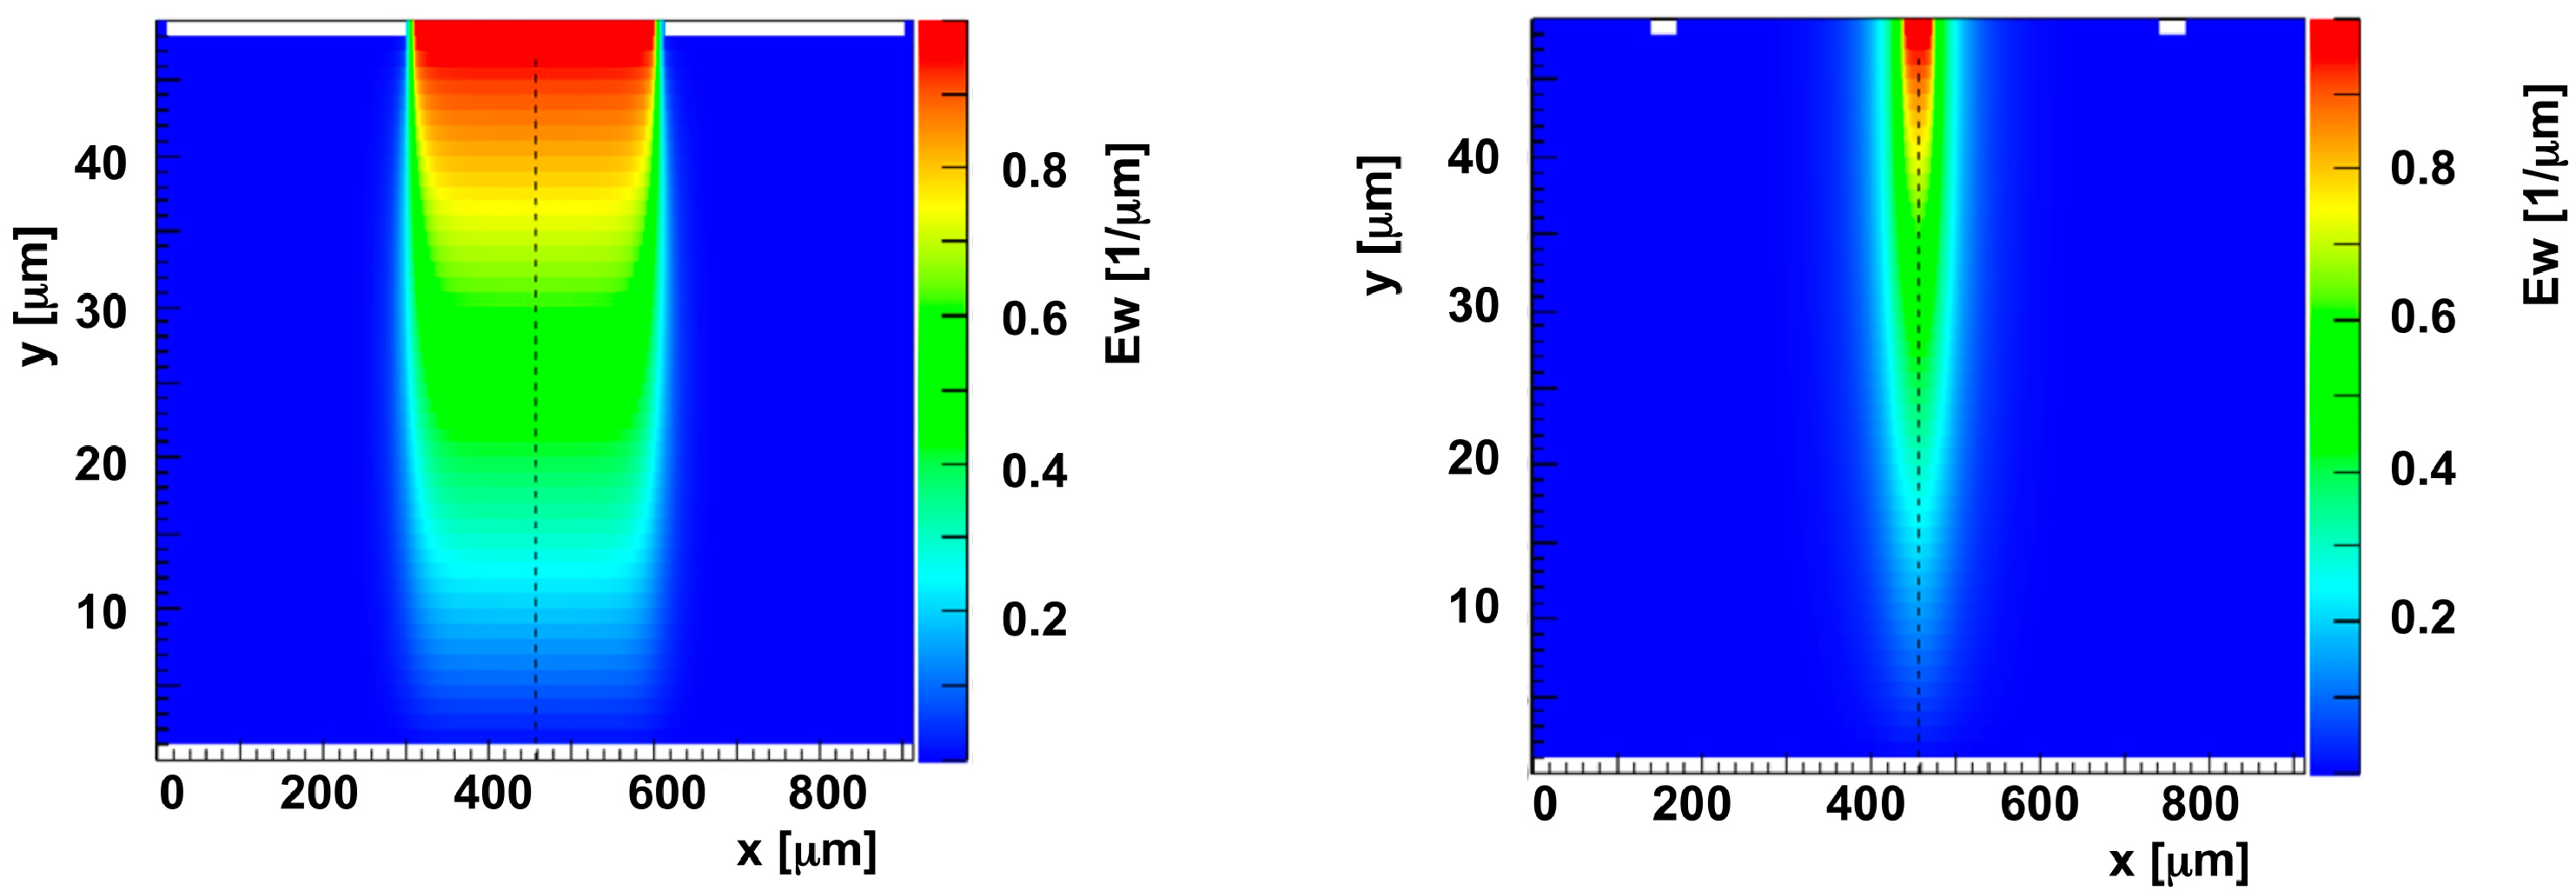
\includegraphics[width=0.85\linewidth]{files/weighting_field_simulation}
				\caption{Comparison of the weighting field from the large collection electrode (left) and small collection electrode (right). The homogeneity of the field as a function of the $x$ position below the electrode is much better for the large collection electrode. }
				\label{im:weighting_field_simulation}
			\end{figure}
		\end{itemize}
		
		Both parameters point towards the same direction regarding the geometry of the active volume: the ratio between the size of the electrode and the depth of the active volume has to be as big as possible in order to get as close as possible to the ideal parallel plate capacitor, providing homogeneity of drift velocity and weighting field. A small active volume thickness is also compatible with a large weighting field. Unfortunately, a trade-off has once again to be made, a large collection electrode and very thin active volume increases the sensor capacitance, hence increasing the noise in the input of the amplifier. In order to obtain the best possible performance, a tailored design of each key detector characteristics has to be made. 
		
		A last contribution to the time resolution arises from the digitisation of the time itself. Indeed the information is typically performed in a Time-to-Digital Converter (TDC) for which the time of the leading edge of the discriminator is digitised and the information is then stored in a time bin defined by the TDC Least Significant Bit (LSB) \cite{timepix4}. If the time bins have a width $\Delta t$ then the contribution to the time resolution is of the order of: 
		\begin{equation}
			\sigma_{\text{TDC}} = \frac{\Delta t}{\sqrt{12}}
		\end{equation}
		
		In the following discussion, the time associated to the different sampling points of the waveforms registered by the oscilloscope with a sampling rate of 40 GS/s, resulting in a time bin width of $\Delta t = $ \SI{25}{\pico\second} and so a contribution to the time resolution $\sigma_{\text{TDC}} =$ \SI{7}{\pico\second}. A simple interpolation between consecutive sampling points helps reducing by an additional factor 2 this contribution, hence making it insignificant for the time resolution measured with the \textit{ATTRACT} and \textit{MONOLITH} prototypes. 
	\clearpage
	
	
	
	
%	\section{Test Beam at the CERN SPS Facility \textcolor{blue}{ 17 pages}}
%	The characterisation of the performance in terms of time resolution and detection efficiency is usually performed using a focused beam of particles behaving like MIPs. As these particle deposit the minimum amount of energy through ionisation, they constitute the perfect probe to estimate the performance of a detector as they provide the minimum possible energy any ionising particle could deposit. Additionally, particles in a wide range of energies behave almost like a MIP, hence providing a description of the performance relative to a wide category of particles. 
%	
%	At CERN, the proton are injected into the LHC by the Super Proton Synchrotron (SPS) a \SI{6.9}{\kilo\meter} long circular accelerator capable of delivering proton with an energy up to \SI{450}{\giga\electronvolt}. While the LHC doesn't need to be filled, the proton accelerated in the SPS can serve a different purpose, such as providing the North Area site in Prévessin with protons. The beam is split and sent into different target, producing a wide range of particles later sent into 4 different beam-lines in the experimental hall. In the work presented in this section, a beam of pions with momentum of 120 GeV/c and 180 GeV/c has been used respectively for the characterisation of the prototypes \textit{ATTRACT} and \textit{MONOLITH} prototypes. \\
%	
%	At first a general description of the experimental set-up used throughout the different data taking campaigns will be presented along with some specificities for the three of them. The procedure progressively improved with time and experience, making the procedure more efficient, robust and precise. 
%	The advantage of a testbeam is also to be able to perform position dependent measurement of the many performances indices of the Device Under Test (DUT) through the use of a particle telescope. This instruments allows to reconstruct the particles tracks from the beam and reconstruct their impinging position on the DUT. A description of the instrument used in this work as well as an explanation of how tracks reconstruction was performed will be given. 
%	Matching of the events recorded by the particle telescope and the waveforms recorded in the oscilloscope from the DUTs and other reference sensors will be explained along with the diverse selection criteria in order to produce a clean sample for analysis. Throughout this work, many different analysis methods for the time resolution notably were investigated and will be discussed in details. 
%	Finally, the results in terms of detection efficiency and time resolution for the \textit{ATTRACT} and \textit{MONOLITH} prototypes will be presented, highlighting the progress made in terms or performance from one prototype to the other. 
%	
%		\subsection{Layout of Test Beam Experiment \textcolor{red}{ 2 pages}} 
%		\subsection{The FE-I4 Telescope: Track Reconstruction \textcolor{red}{ 2 pages}}
%		\subsection{Dataset Construction and Analysis Methods \textcolor{red}{ 3 pages}}

	\section{Particle Telescope and Track Reconstruction \textcolor{red}{ 2 pages}}

	\clearpage
	\section{Test Beam Characterisation of \textit{ATTRACT} Prototypes}
		The \textit{ATTRACT} prototype was first tested in the laboratory at the University of Geneva through the course of late 2020 and early 2021 for a first characterisation of the frontend's amplifier performance as well as an estimation of the time resolution using a source of \Sr and a Low Gain Avalanche Diode (LGAD) for time reference, the results were presented in \cite{Moretti_MasterThesis}.
		
		In July 2021, a test beam campaign was organised at the CERN SPS North Area experimental hall. The beam used to qualify the two nearly identical \textit{ATTRACT} prototypes was composed of pions with a momentum of \SI{180}{\giga\electronvolt}/c a beam spread of about a few millimetres wide and very straight tracks (almost no beam divergence). The track position on the Device Under Test (DUT) were reconstructed using the FE-I4 UniGe telescope \cite{telescope} and allowed for a mesure of the detection efficiency as a function of the particle position within the pixel. The time resolution was also estimated using the two prototypes under the assumption that their timing performance was equivalent. 
		
		The results are presented for the prototypes as a function of the power density (\power) and as a function of the High Voltage (HV) bias  given to the substrate. The following section refers to the work published in early 2022 in the Journal of Instrumentation (JINST) \cite{ATTRACT_proto1_testbeam}. 
		
		\subsection{frontend Calibrations}

		Laboratory measurements with X-ray sources were performed to characterise the analog response of the frontend electronics of two ASICs, that will be called here Device Under Test 0 (DUT0) and 1 (DUT1). For these measurements and those described in Section \note{section ref}, the outputs of the analog drivers were connected to a \SI{50}{\ohm} coaxial cable and AC coupled via a \SI{100}{\nano\farad} capacitor to a Lecroy WaveMaster 820zi oscilloscope. The oscilloscope has a sampling rate of 40 Gs/s and its analog bandwidth was limited to 4 GHz. 
		A \Cd source was used to measure the gain of the electronic chain, which includes the pixel, the preamplifier and the driver. To study the response of the electronics as a function of the power density, four different working points were adopted, with  amplifier bias current $I_{\text{preamp}} = $  \SI{7}{\micro\ampere}, \SI{20}{\micro\ampere}, \SI{50}{\micro\ampere} and \SI{150}{\micro\ampere} respectively resulting in power densities of \power = \SI{0.08}{\watt/\centi\meter^2}, \SI{0.24}{\watt/\centi\meter^2}, \SI{0.60}{\watt/\centi\meter^2}, \SI{1.8}{\watt/\centi\meter^2}.
		\begin{figure}[h]
			\centering
			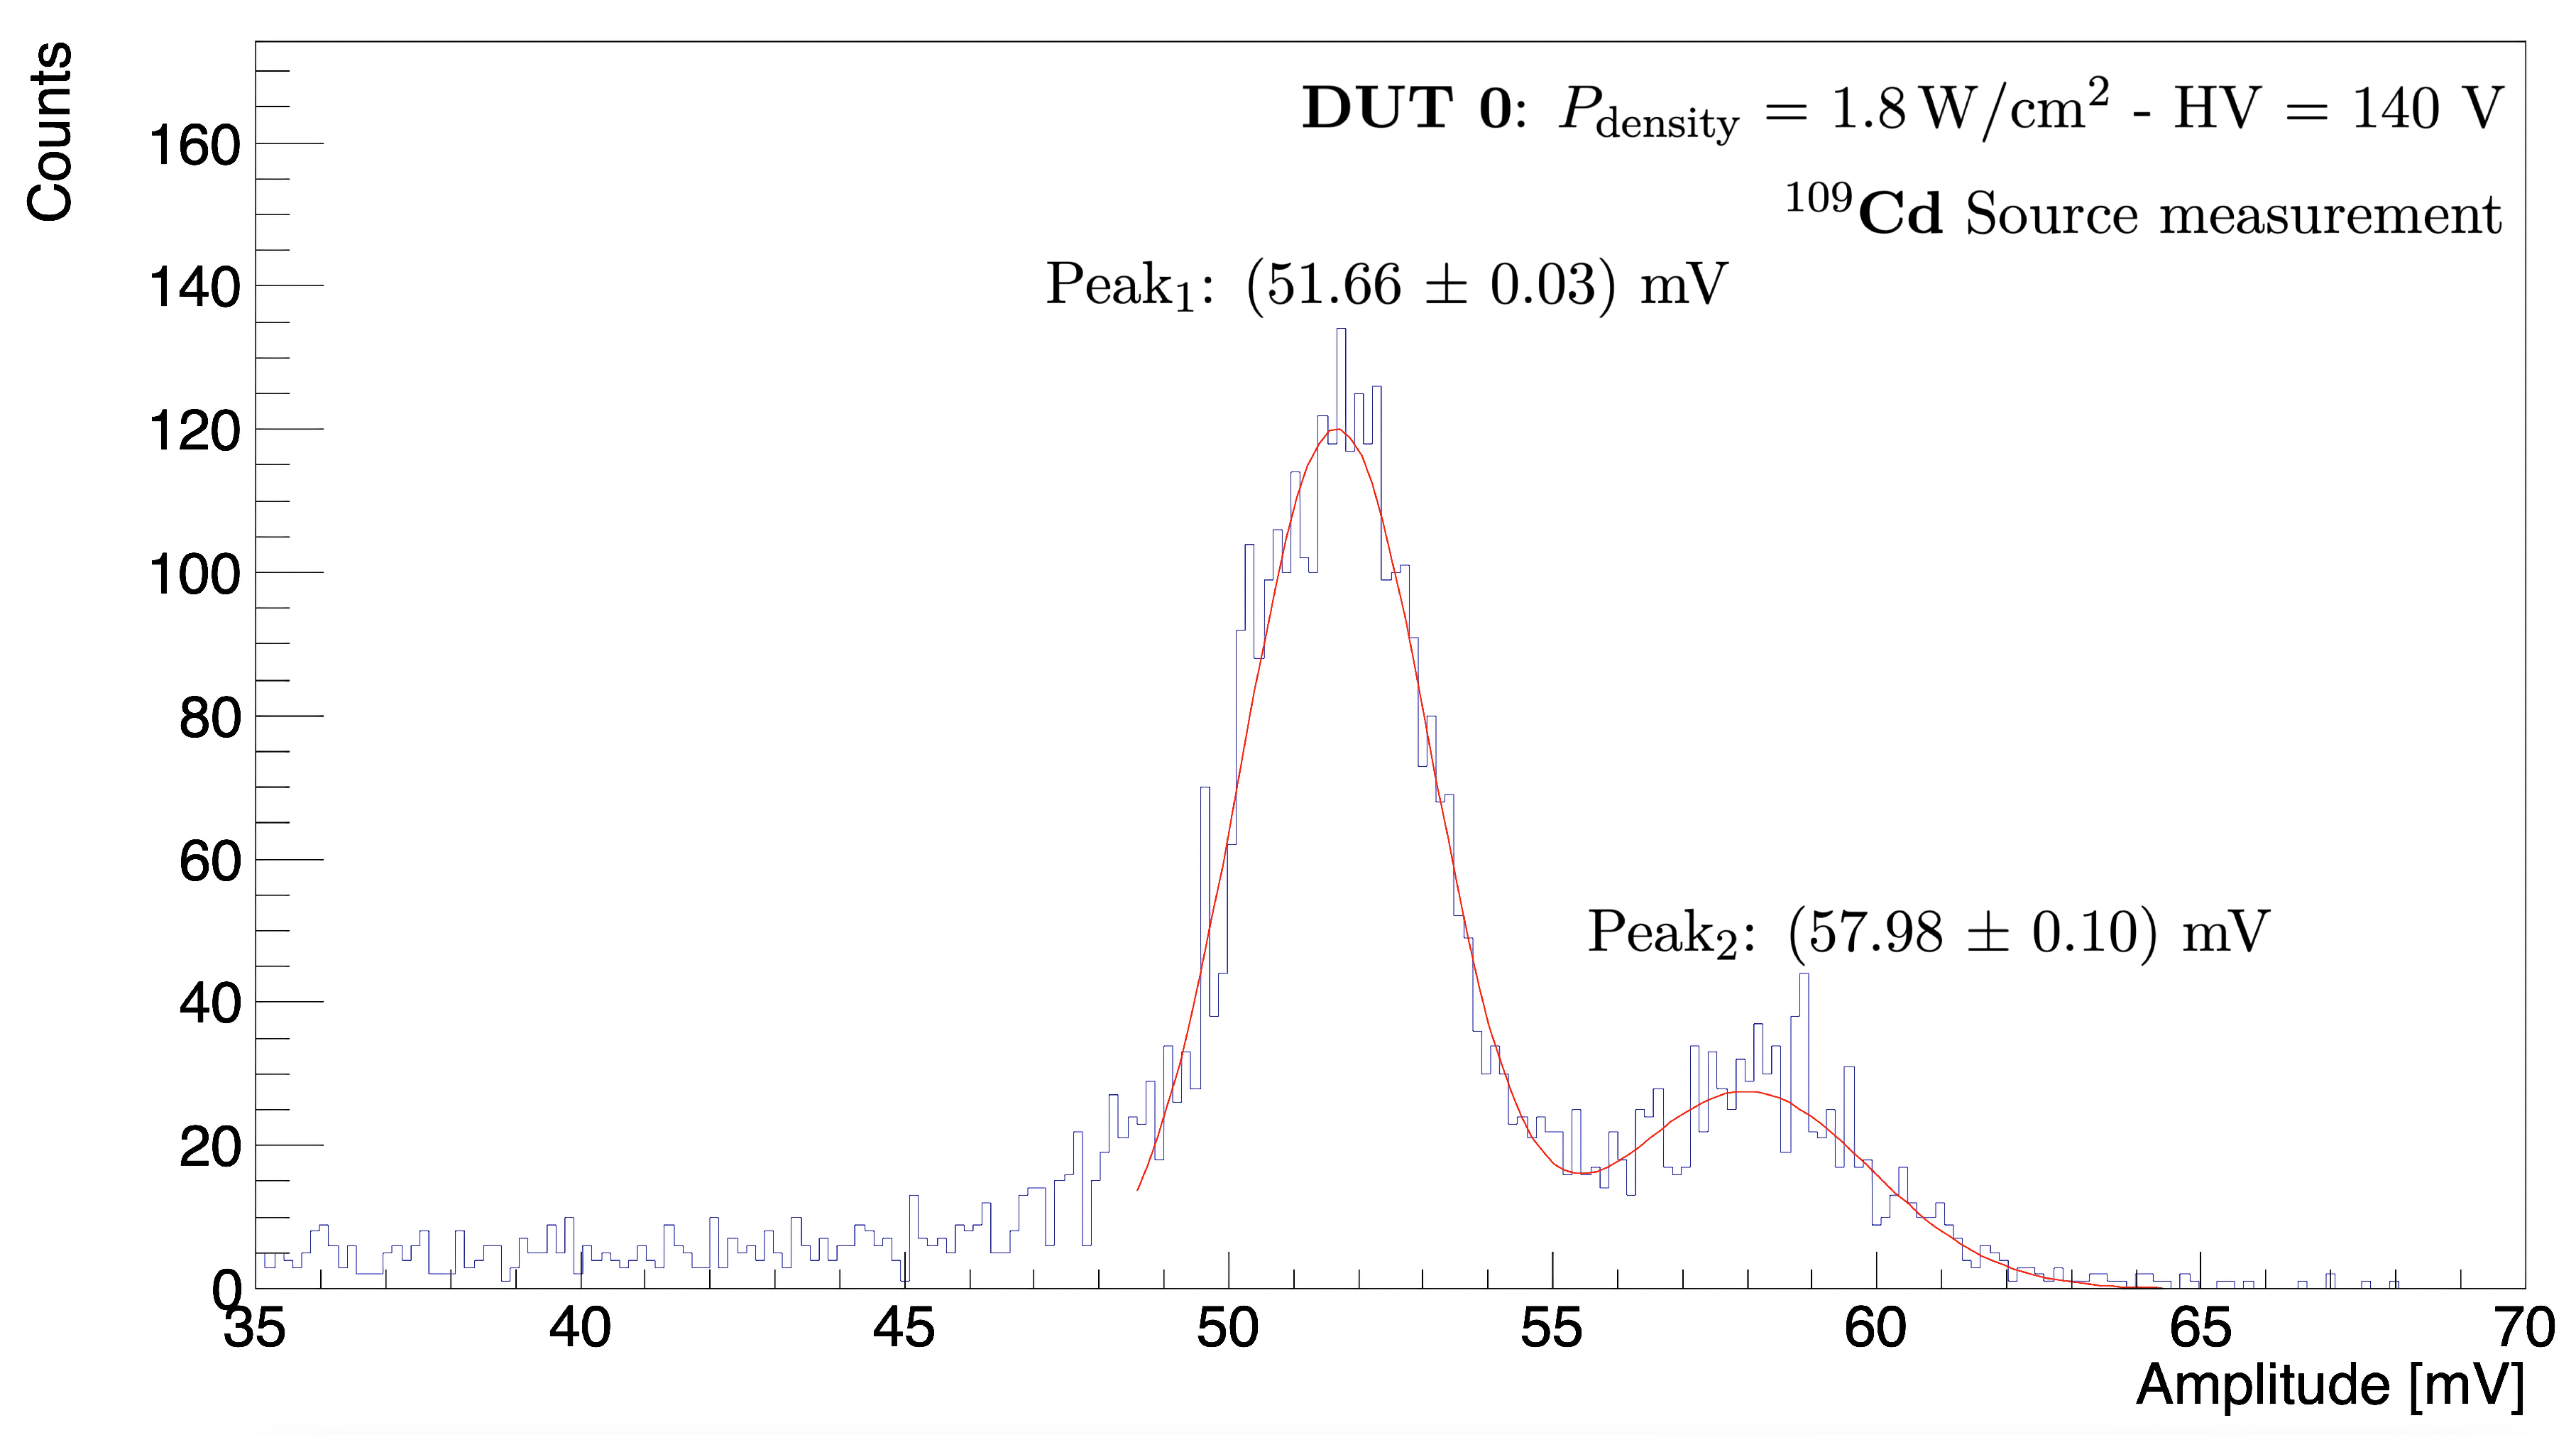
\includegraphics[width=0.88\linewidth]{files/ATTRACT_paper/Cd109_SpectrumAnalysis}
			\caption{Spectrum of the \Cd source measured at the working point \power = \SI{1.8}{\watt/\centi\meter^2} and $HV=140~V$. The two peaks, corresponding to the X-ray emission of $^{109}Ag$,  were fitted with a double Gaussian function.}
			\label{im:ATTRACT_CdSpectrum}
		\end{figure}
		
		The two main photons from the \Cd source derive from the $ ^{109}Ag $ X-ray K lines of energy $E_{1} = \SI{22.16}{\kilo\electronvolt}$ and $E_{2} = \SI{24.94}{\kilo\electronvolt} $.
		The spectrum of \Cd was fitted with a double Gaussian function. Figure \ref{im:ATTRACT_CdSpectrum} shows one example of the spectra from DUT0, while Figure \ref{im:ATTRACT_CdFit} shows the amplitude values obtained from the fit of the same spectrum as a function of the deposited charge, assuming an energy of \SI{3.6}{\electronvolt} to generate and electron-hole pair in silicon. A linear fit of the data was used to estimate the charge gain ($ A_q $) of the frontend electronics. 
		
		
		\begin{figure}[h]
			\centering
			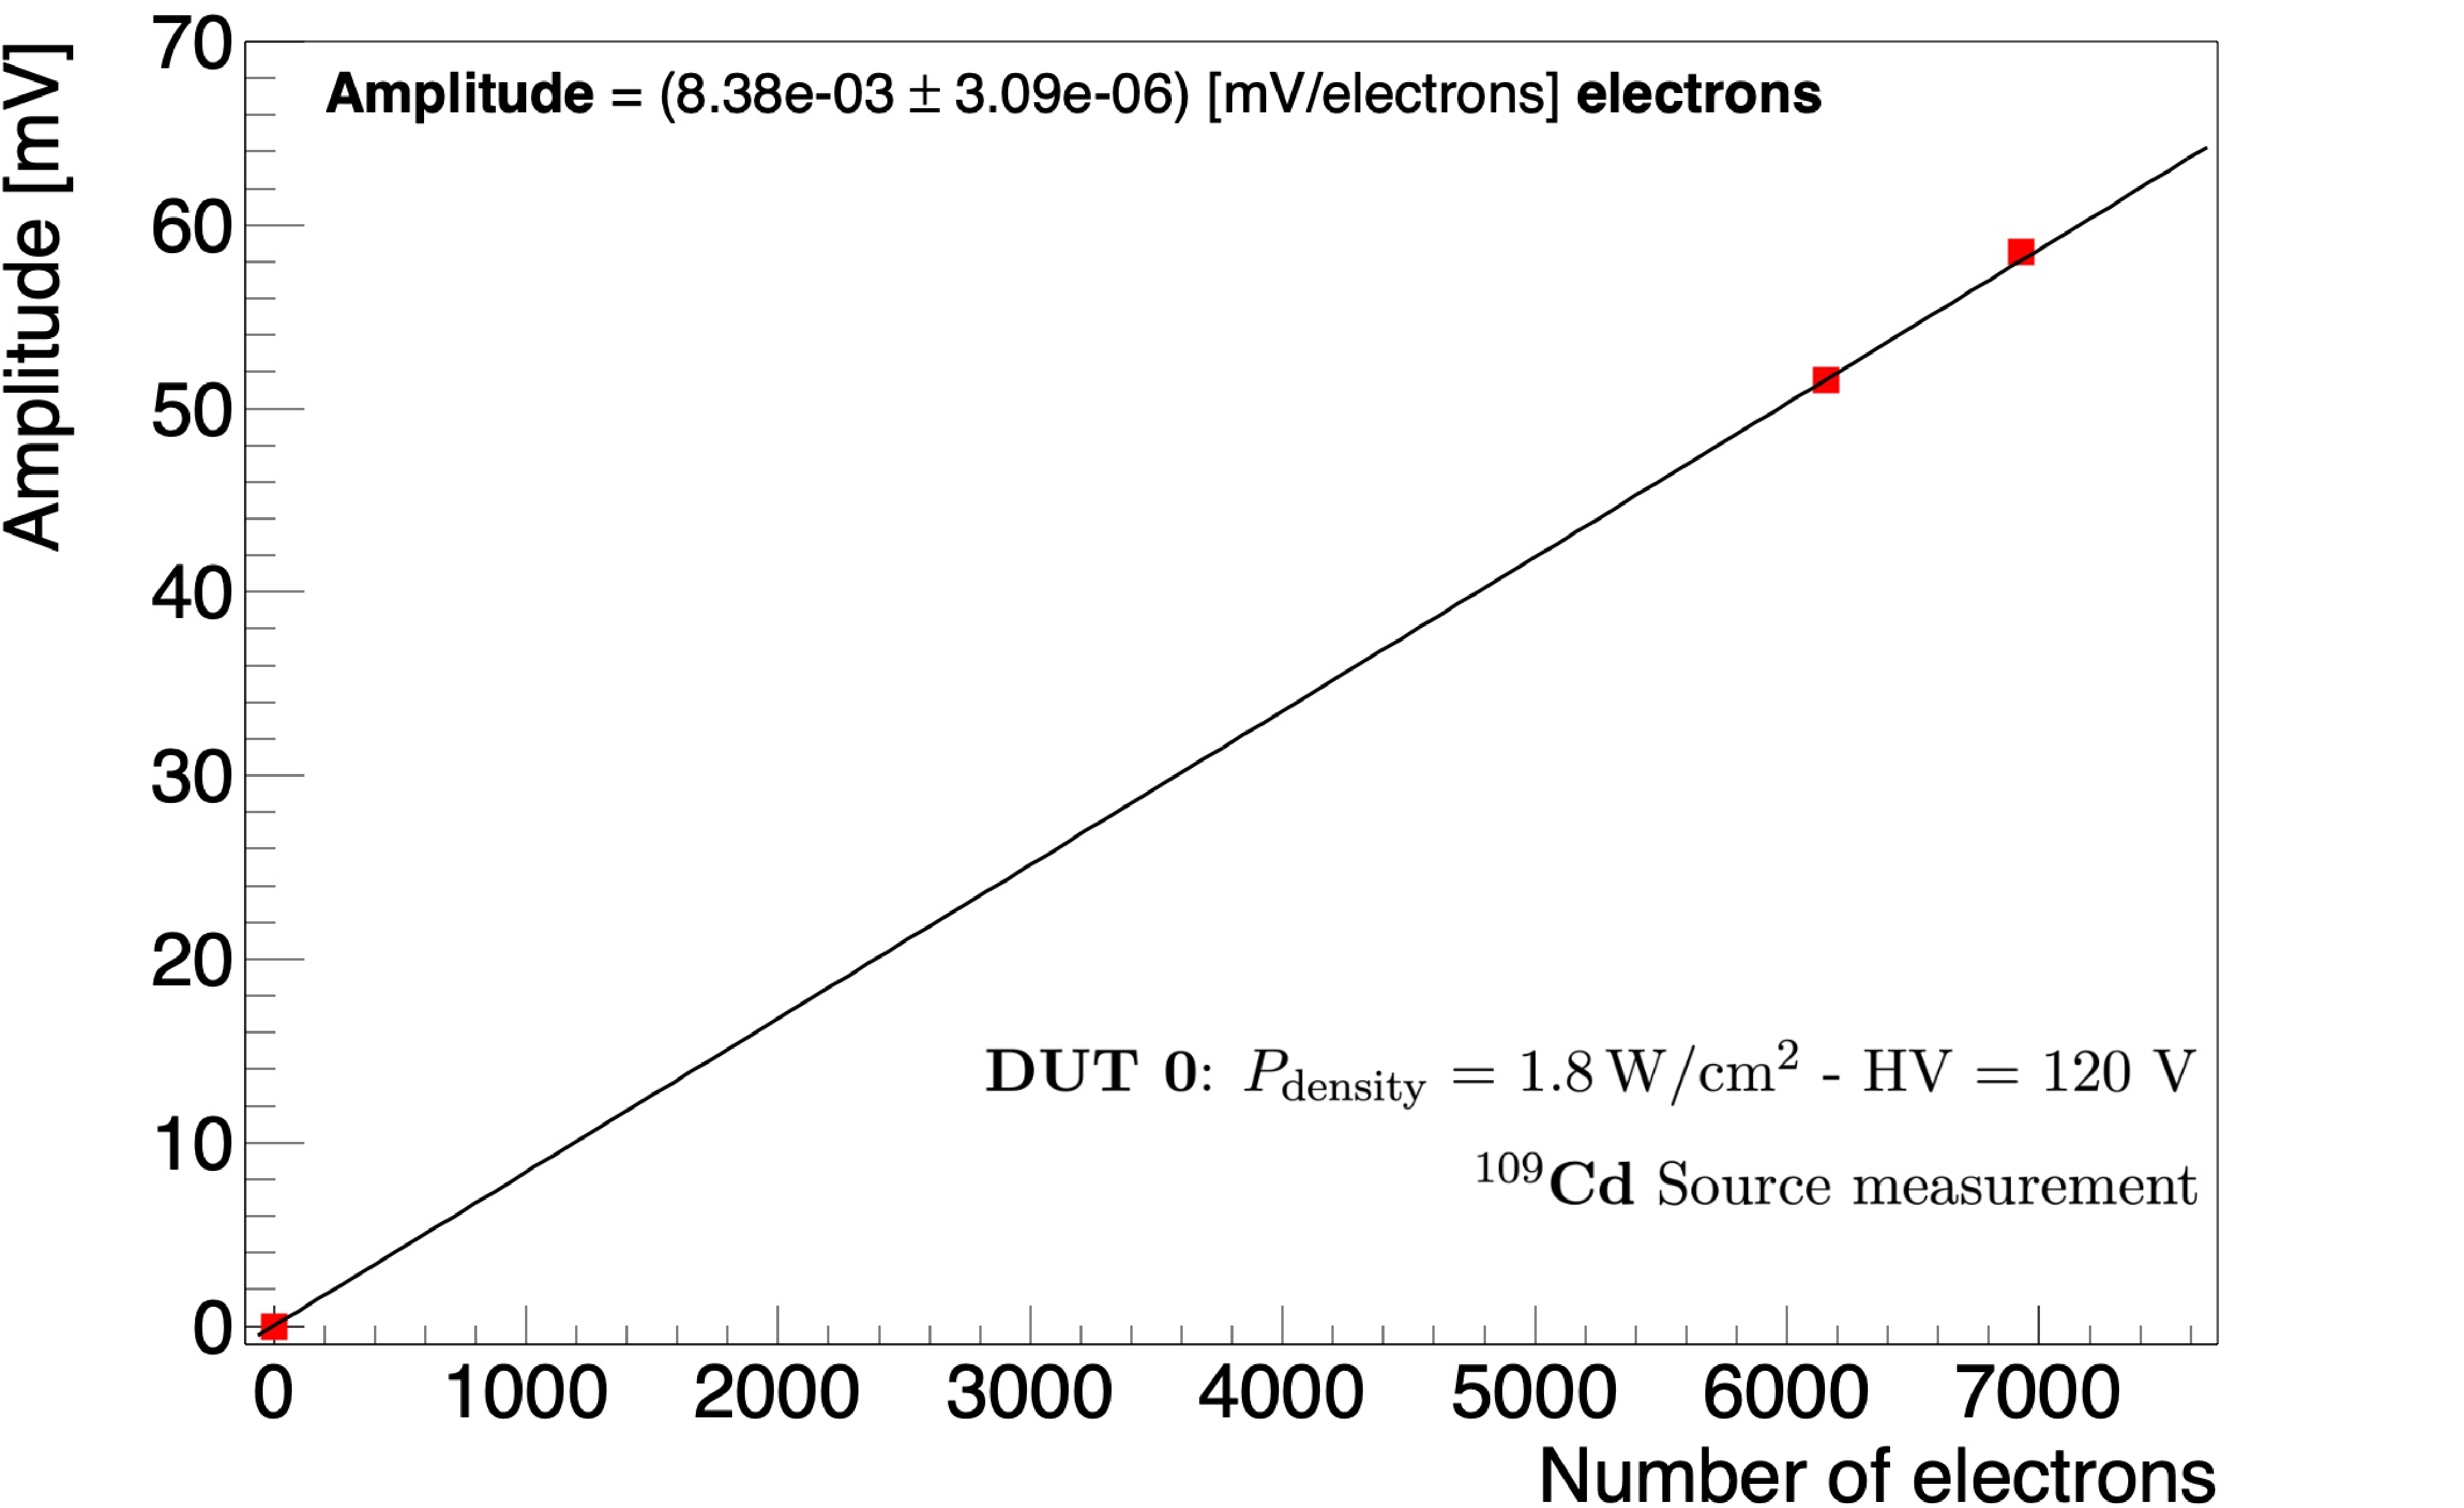
\includegraphics[width=0.8\linewidth]{files/ATTRACT_paper/Calibration_DUT0_120V_150uA}
			\caption{Example of the amplitude measurement as a function of the number of electrons obtained with the \Cd source for one of the working points for DUT0. The superimposed linear fit  is used to parameterise  the response of the frontend at this working point.}
			\label{im:ATTRACT_CdFit}
		\end{figure}

		The Equivalent Noise Charge (ENC) of the frontend was then calculated as

		\vspace{-3mm}
		\begin{equation*}
			ENC = \frac{\sqrt{\sigma_V^2-\sigma_{\text{scope}}^2}}{A_q}
		\end{equation*}

		\vspace{-1mm}
		where \noise is the standard deviation of the electronics-noise distribution measured on the oscilloscope when the frontend is connected, and $\sigma\_{\text{scope}} =$ \SI{420}{\micro\volt} is the voltage noise of the oscilloscope with the open input connector. The results of the gain and ENC measurements are summarised in Table \ref{tab:ATTRACT_gaintable}. The two DUTs show the same trend within approximately 10\%. At  \power = \SI{0.6}{\watt/\centi\meter^2} the ENC is as low as 50 electrons. As expected, it increases significantly for smaller $ I_{\text{preamp}} $ values, which could produce a degradation of the detection efficiency. The increase of the ENC at \power =  \SI{1.8}{\watt/\centi\meter^2} is due to the configuration of the amplifier used for this working point.

		\begin{table}[h!]
    		\centering
    		\begin{tabular}{c|ccc|ccc|}
    		\cline{2-7}
 			& \multicolumn{3}{c|}{\textbf{DUT0}} & \multicolumn{3}{c|}{\textbf{DUT1}} \\ \hline
    		\multicolumn{1}{|c|}{\begin{tabular}[c]{@{}c@{}}Power density\\ {[}W/cm$^2${]}\end{tabular}} 
    		& \multicolumn{1}{c|}{\begin{tabular}[c]{@{}c@{}}$\sigma_V$\\ {[}mV{]}\end{tabular}} 
    		& \multicolumn{1}{c|}{\begin{tabular}[c]{@{}c@{}}A$_q$\\ {[}mV/fC{]}\end{tabular}} 
    		& \begin{tabular}[c]{@{}c@{}}ENC\\ {[}electrons{]}\end{tabular} 
    		& \multicolumn{1}{c|}{\begin{tabular}[c]{@{}c@{}}$\sigma_V$\\ {[}mV{]}\end{tabular}} 
    		& \multicolumn{1}{c|}{\begin{tabular}[c]{@{}c@{}}A$_q$\\ {[}mV/fC{]}\end{tabular}} 
    		& \begin{tabular}[c]{@{}c@{}}ENC\\ {[}electrons{]}\end{tabular} \\ \hline
    		\multicolumn{1}{|c|}{0.08} & \multicolumn{1}{c|}{1.35} & \multicolumn{1}{c|}{42.3} & 194 $\pm$ 1 & \multicolumn{1}{c|}{1.41} & \multicolumn{1}{c|}{49.2} & 171 $\pm$ 2 \\ \hline
   			\multicolumn{1}{|c|}{0.24} & \multicolumn{1}{c|}{0.82} & \multicolumn{1}{c|}{43.4} & 102 $\pm$ 1 & \multicolumn{1}{c|}{0.83} & \multicolumn{1}{c|}{46.0} & ~97 $\pm$ 1 \\ \hline
    		\multicolumn{1}{|c|}{0.60} & \multicolumn{1}{c|}{0.70} & \multicolumn{1}{c|}{55.0} & ~54 $\pm$ 1 & \multicolumn{1}{c|}{0.58} & \multicolumn{1}{c|}{50.5} & ~50 $\pm$ 1 \\ \hline
    		\multicolumn{1}{|c|}{1.80} & \multicolumn{1}{c|}{0.81} & \multicolumn{1}{c|}{52.4} & ~76 $\pm$ 1 & \multicolumn{1}{c|}{0.72} & \multicolumn{1}{c|}{44.4} & ~82 $\pm$ 1 \\ \hline
    		\end{tabular}
    		\caption{Voltage noise, charge gain and ENC of the analog frontend electronics at the four power density working points for HV = 120 V. The lower ENC value measured at \SI{0.6}{\watt/\centi\meter^2} is due to a different configuration of the amplifier and driver working point that acts as a filter for noise, thus reducing the bandwidth.}
    		\label{tab:ATTRACT_gaintable}
		\end{table}

		
		
		\subsection{Testbeam experiment setup and data set}

		The detection efficiency and time resolution of the prototypes were measured at the CERN SPS testbeam facility with a pion beam with \SI{180}{\giga\electronvolt}/c momentum. The experimental setup consisted of the UniGe FE-I4 telescope for particle tracking \cite{telescope}, with the two devices under test (DUT0 upstream with respect to the beam, DUT1 downstream) placed after three detection planes of the telescope as shown in Figure \ref{im:ATTRACT_Setup}. The DUTs were operated at room temperature. The DUTs were readout by two oscilloscopes with analog bandwidth of 4 GHz and a sampling rate of 40 GS/s and 20 GS/s, respectively. The DUTs were positioned specularly to each other and pixels OA0 (shown in Figure \ref{im:ATTRACT_ASIC_layout}) from the two chips were aligned and sent to the oscilloscope with the largest sampling rate to make Time-Of-Flight (TOF) measurements. The data from pixels OA1 and OA2 of the two DUTs, which were not aligned among the two DUTs, were also acquired.

		\begin{figure}[h]
			\centering
			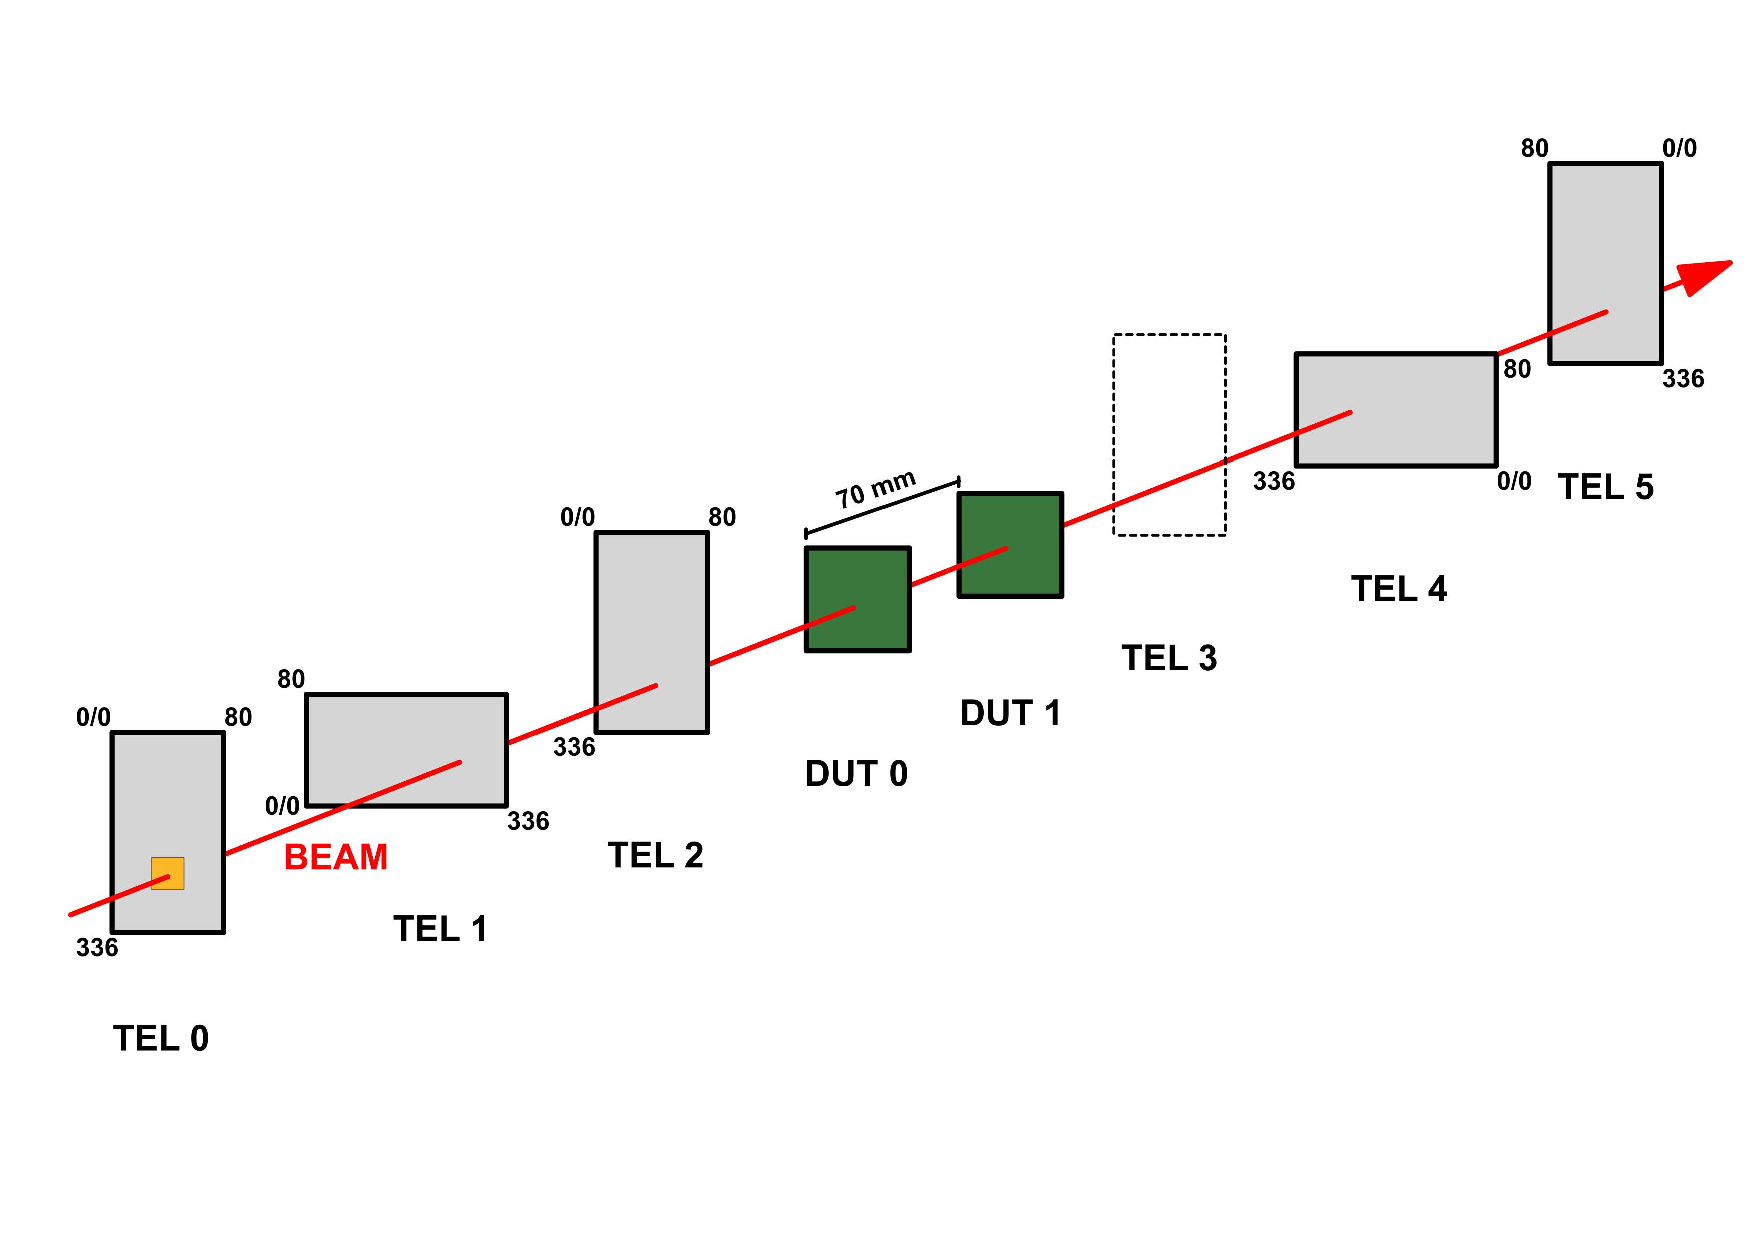
\includegraphics[width=0.75\linewidth]{files/ATTRACT_paper/Setup_reprint.pdf}
			\caption{Schematic view of the experimental setup, showing the five FE-I4 telescope \cite{telescope} planes that were operated and the two DUTs in green. Plane TEL3 was not operational during this testbeam measurement. The FEI4 readout chip has a matrix of $ 80 \times 336 $ pixels with a pixel size of $ 250 \times 50 ~\si{\micro\meter\squared} $. The telescope planes are alternatively rotated by 90$^\circ$ to optimise the space resolution on the two transversal directions. A region of interest, shown by the yellow area, was imposed to the first plane of the telescope, and was put in coincidence with the last telescope plane to generate the trigger.}
			\label{im:ATTRACT_Setup} 
		\end{figure}

		The analysis of the data was performed using the full waveform information acquired by the oscilloscopes. The signals from the DUTs were delayed to guarantee that they were always in the second half of the waveform time window acquired by the oscilloscope.
		This configuration allowed using the first half of the waveform to determine the voltage noise \noise at the output of the analog frontend and set a discrimination threshold $V_{th}$ as a multiple of the voltage noise, independently for the two DUTs. Figure~\ref{im:ATTRACT_waveform} shows a typical waveform with a signal pulse from a MIP at the working point with  \power = \SI{1.8}{\watt/\centi\meter^2}. The dashed line represents the discrimination threshold at $V_{th}=6$ \noise.

		\begin{figure}[h]
			\centering
			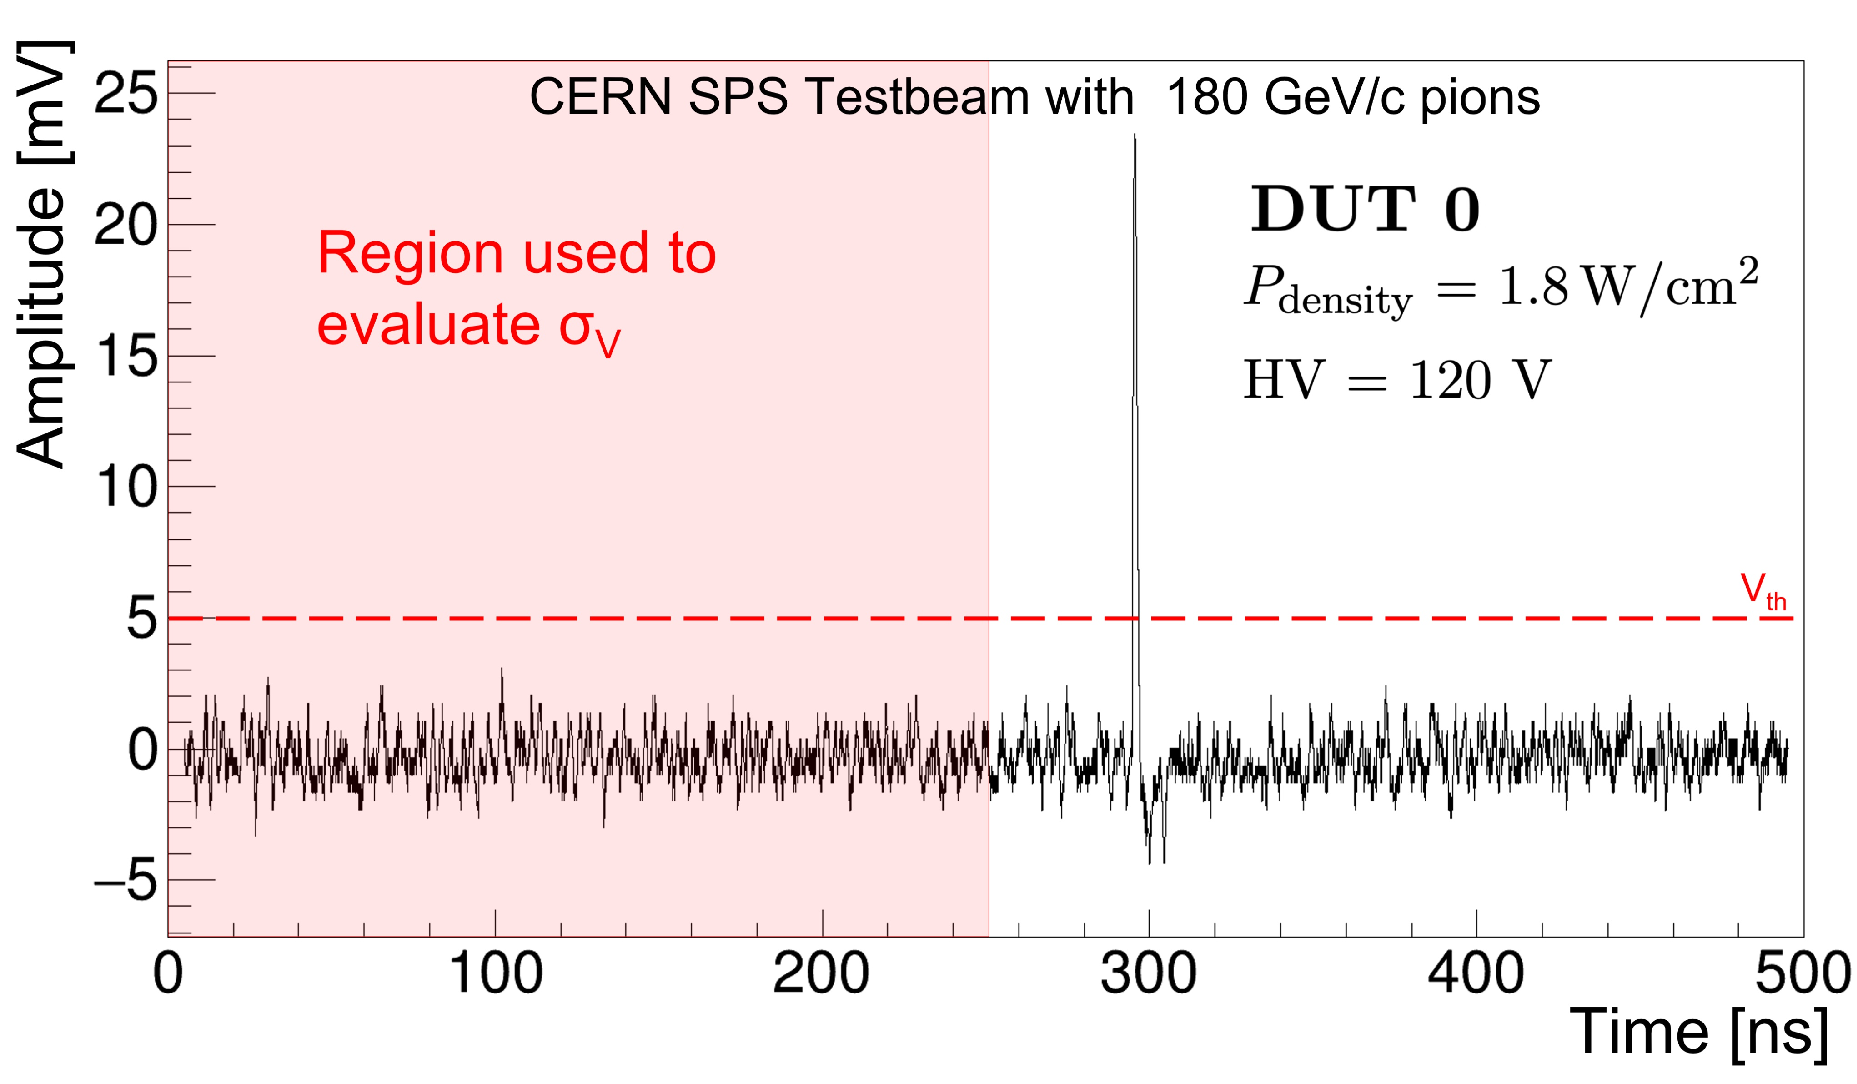
\includegraphics[width=0.75\linewidth]{files/ATTRACT_paper/Waveform_analysis}
			\caption{Example of a waveform from working point \power = \SI{1.8}{\watt/\centi\meter^2}. The shaded region below \SI{250}{\nano\second} is the portion of the waveform used to extract \noise. The dashed line shows the discrimination threshold used for this working point.}
			\label{im:ATTRACT_waveform} 
		\end{figure}

		The FE-I4 telescope provided the trigger to the oscilloscopes. A Region Of Interest (ROI) of $ 250 \times 600 $  $\mu$ m$^2$ was set on one of the trigger planes of the telescope, centred around the pixels OA0 of the two DUTs that were aligned with respect to the beam line and used for the TOF measurement.
		Data samples were acquired with DUT0 and DUT1 at the same four frontend working points used for the characterisation of the DUTs with radioactive sources (\note{section ref}) for a high voltage bias of 120 V. At this potential the substrate is not fully depleted. The depletion depth is estimated to be \SI{23}{\micro\meter}, which corresponds to a most probable charge $ Q_{MPV} \approx 1300 $ electrons for a MIP. 

		A high voltage scan was also performed only for the working point \power = \SI{1.8}{\watt/\centi\meter^2}. 
		To evaluate the efficiency and time resolution of the DUTs in the cleanest possible way, a selection was applied on the quality of the tracks reconstructed by the FE-I4 telescope. The selection consisted in discarding events in which more than one track was reconstructed by the telescope, and in accepting only events with the reconstructed track having an associated hit in each of the five telescope planes and a $ \chi^{2}/NDF \le 1 $. About 30\% of the triggered events survived this stringent selection on the tracks from the telescope. For this final sample the telescope pointing resolution on the DUT planes was estimated to be approximately 10 $\mu$m in both directions \cite{vicente_thesis}.

		\subsection{Cross talk and robustness to induced noise}
		During laboratory and testbeam measurements, cross talk between the channels was observed for events with large charge deposition, corresponding to approximately five times the MIP most probable charge. The analysis of these events showed that this cross talk was not influenced by the relative position of the pixels within the matrix or the routing of the signal before and after the amplification. Therefore the observed cross talk could be ascribed to two possible causes. The first is a feedback path passing through the ground of the Printed Circuit Board (PCB), which is then injected to the backside of the chip through the HV decoupling capacitors and finally in the amplifier input. This hypothesis is supported by the fact that the system becomes less stable at high voltage biases below \SI{50}{\volt}, when the pixel capacitance is significantly larger. The second cause is noise induced by the driver pulse propagating in the power supply, since in this prototype the analog and driver electronics share the same supply lines.

		As a consequence of this cross talk, only  events in which the pixel under test had the largest signal among the three acquired pixels were selected for the time resolution measurement. No selection was applied for cross talk in the efficiency measurement, since cross talk appears only for efficient events.

		\subsection{Detection efficiency}
		For the calculation of the efficiency, all the selected pion tracks reconstructed by the FE-I4 telescope were extrapolated to the surface of each of the two DUTs. Only the tracks crossing a DUT within the  area of the three pixels under study, or outside the  external edges of the pixels by at most one standard deviation of the telescope resolution, were retained. An event was considered efficient if the signal in at least one of the three pixels crossed the discrimination threshold.

		Figure \ref{im:ATTRACT_effmap} shows the efficiency map for the two DUTs at the \power = \SI{1.8}{\watt/\centi\meter^2} working point, for a threshold of 6\noise and a sensor bias $HV = $ \SI{120}{\volt}. 
		The panels show the efficiency map for the entire surface of the three pixels (the pixel edges are represented by the black lines). The degraded efficiency measured nearby the twelve external sides of the hexagonal pixels is produced by the FE-I4 telescope resolution, as attested by the fact that such degradation of the efficiency is not observed in the region of the three internal hexagon sides between the pixels. 

		\begin{figure}[h]
			\centering
			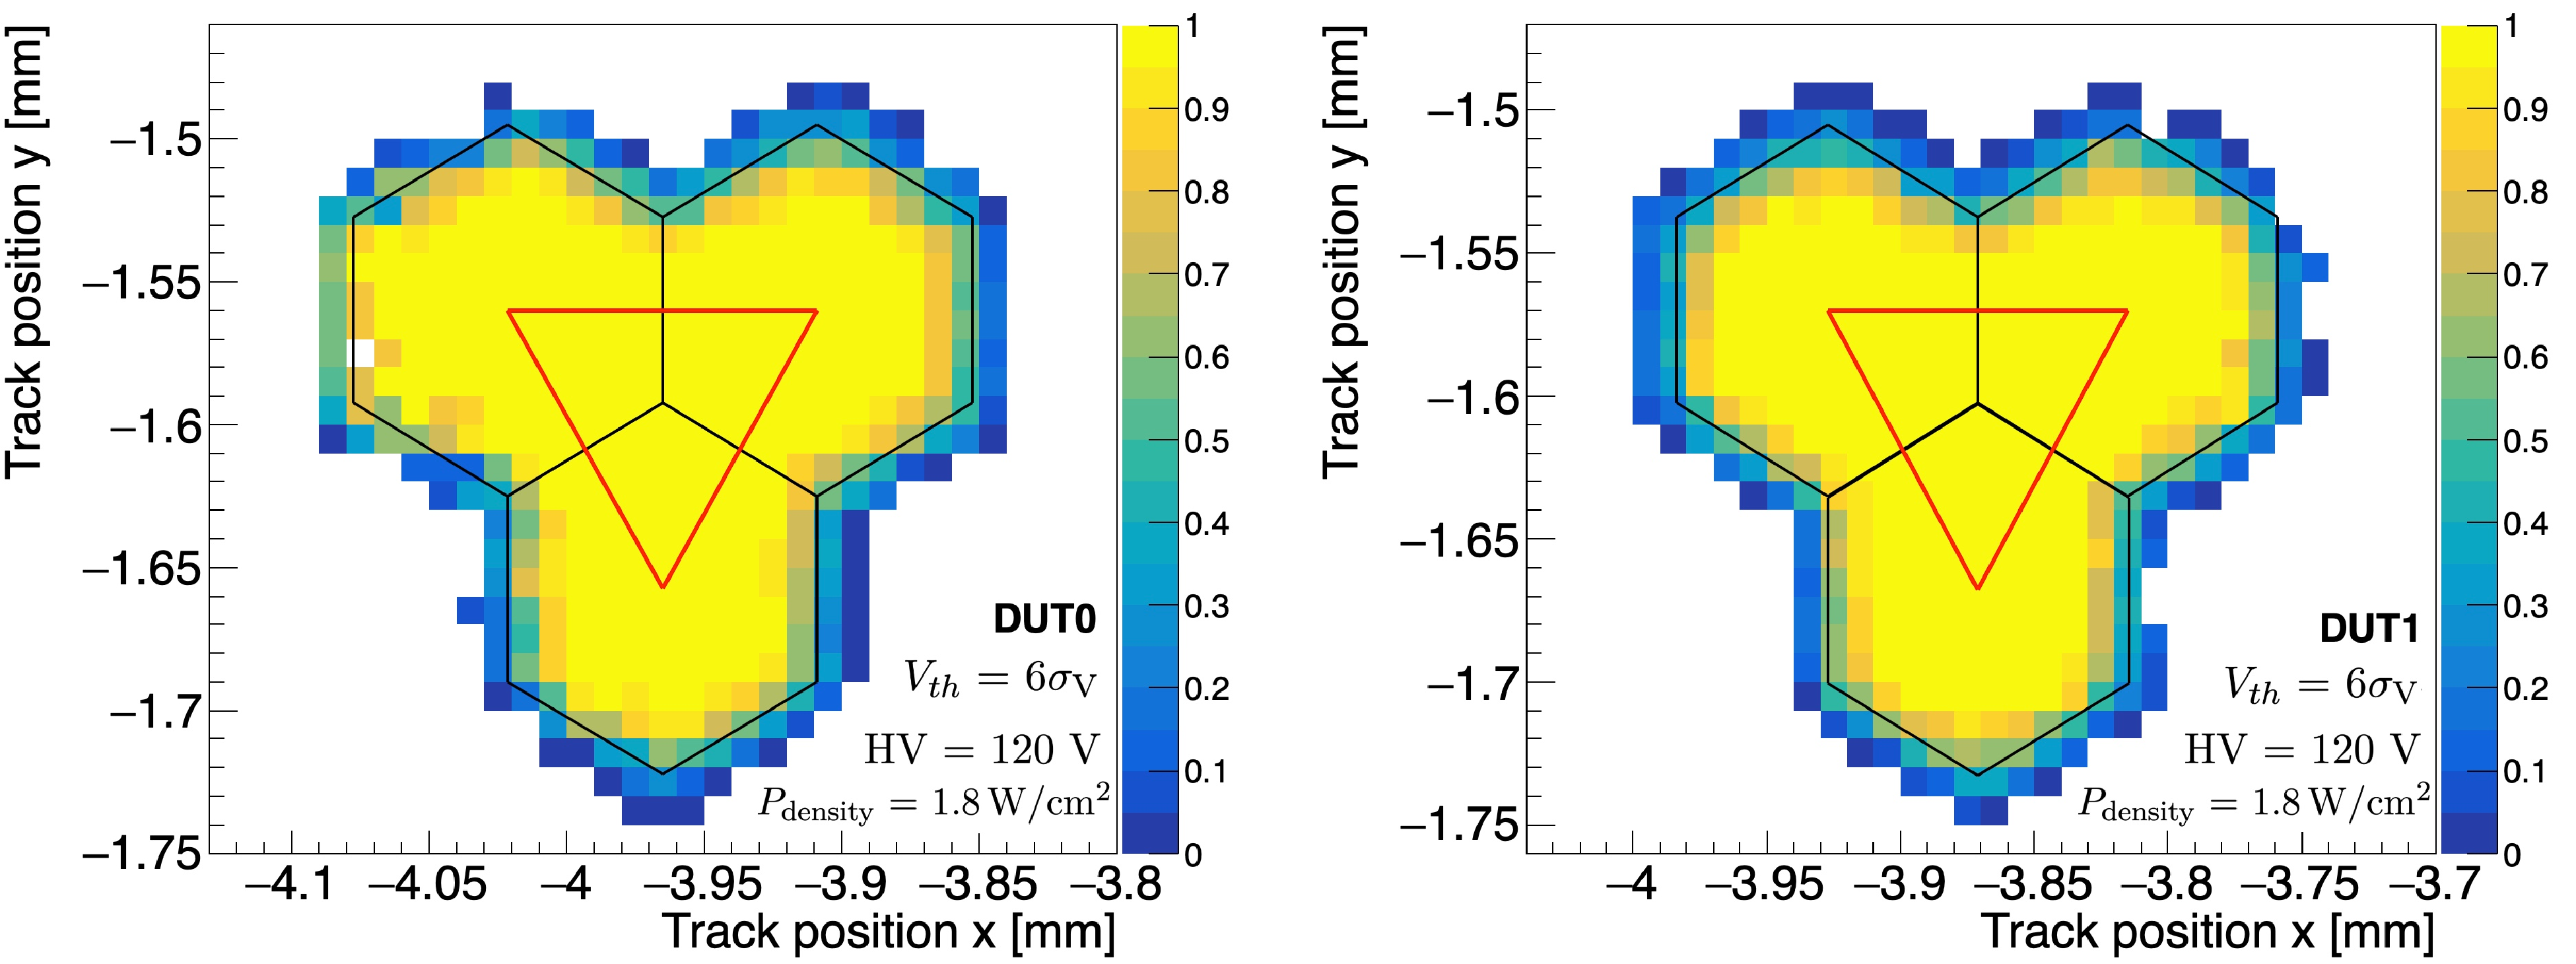
\includegraphics[width=0.99\linewidth]{files/ATTRACT_paper/EfficiencyMap_120V_150uA}
			\caption{Efficiency map measured for DUT0 (left) and DUT1 (right) at  \power = \SI{1.8}{\watt/\centi\meter^2}, threshold $ V_{th} = 6$\noise and $HV$ = \SI{120}{\volt}. The pixel edges are shown by the black lines. The efficiency degradation around the external edges of the three pixels is due to the FE-I4 telescope resolution. The efficiency measured inside the triangular area delimited by the red lines is unaffected by the telescope pointing resolution and is used throughout this study.}
			\label{im:ATTRACT_effmap} 
		\end{figure}
		
		To avoid biases stemming from the pointing resolution of the FE-I4 telescope, the measurement of the detection efficiency was restricted to events with tracks extrapolated inside the triangular area in between the three pixels that is delimited by the red lines in Figure \ref{im:ATTRACT_effmap}. It should be noted that this triangular area constitutes exactly one sixth of the total area of the three pixels, which is representative of all the zones of a pixel (central-pixel zone; zone in between two pixels; zone in between three pixels) in the right geometrical proportions. Therefore, the efficiency measured inside it provides a reliable estimation of the efficiency over the entire hexagonal pixel area, unbiased by the telescope resolution.
		
		\begin{table}[h]
			\centering
			\renewcommand{\arraystretch}{1.3}
			\begin{tabular}{c|cccc|l}
				\cline{1-5}
				\multicolumn{5}{|c|}{Efficiency measured at HV = 120 V}                                                                                                                         & \multicolumn{1}{c}{\textbf{}} \\ \cline{1-5}
				\multicolumn{1}{|c|}{\power [W/cm$^2$]} & \multicolumn{1}{c|}{0.08} & \multicolumn{1}{c|}{0.24} & \multicolumn{1}{c|}{0.60} & 1.80 &                               \\ \cline{1-5}
				\multicolumn{1}{|c|}{Efficiency DUT0 {[}\%{]}} & \multicolumn{1}{c|}{$ 96.1_{-1.7}^{+1.4} $} & \multicolumn{1}{c|}{$ 99.75_{-0.17}^{+0.12} $} & \multicolumn{1}{c|}{$ 99.94_{-0.05}^{+0.03} $} & $ 99.91_{-0.08}^{+0.05} $ &                               \\ \cline{1-5}
				\multicolumn{1}{|c|}{Efficiency DUT1 {[}\%{]}} & \multicolumn{1}{c|}{$ 98.4_{-0.4}^{+0.3} $} & \multicolumn{1}{c|}{$ 99.45_{-0.2}^{+0.2} $}   & \multicolumn{1}{c|}{$ 99.86_{-0.07}^{+0.05} $} & $ 99.78_{-0.11}^{+0.08} $ &                               \\ \cline{1-5}
			\end{tabular}
			\caption{Efficiency of the two DUTs at different \power for $ HV =$ \SI{120}{\volt}. The efficiency is measured according to the definition given in the text. The uncertainties are statistical only.}
			\label{tab:ATTRACT_efftable}
		\end{table}
		
		\begin{figure}[h]
			\centering 
			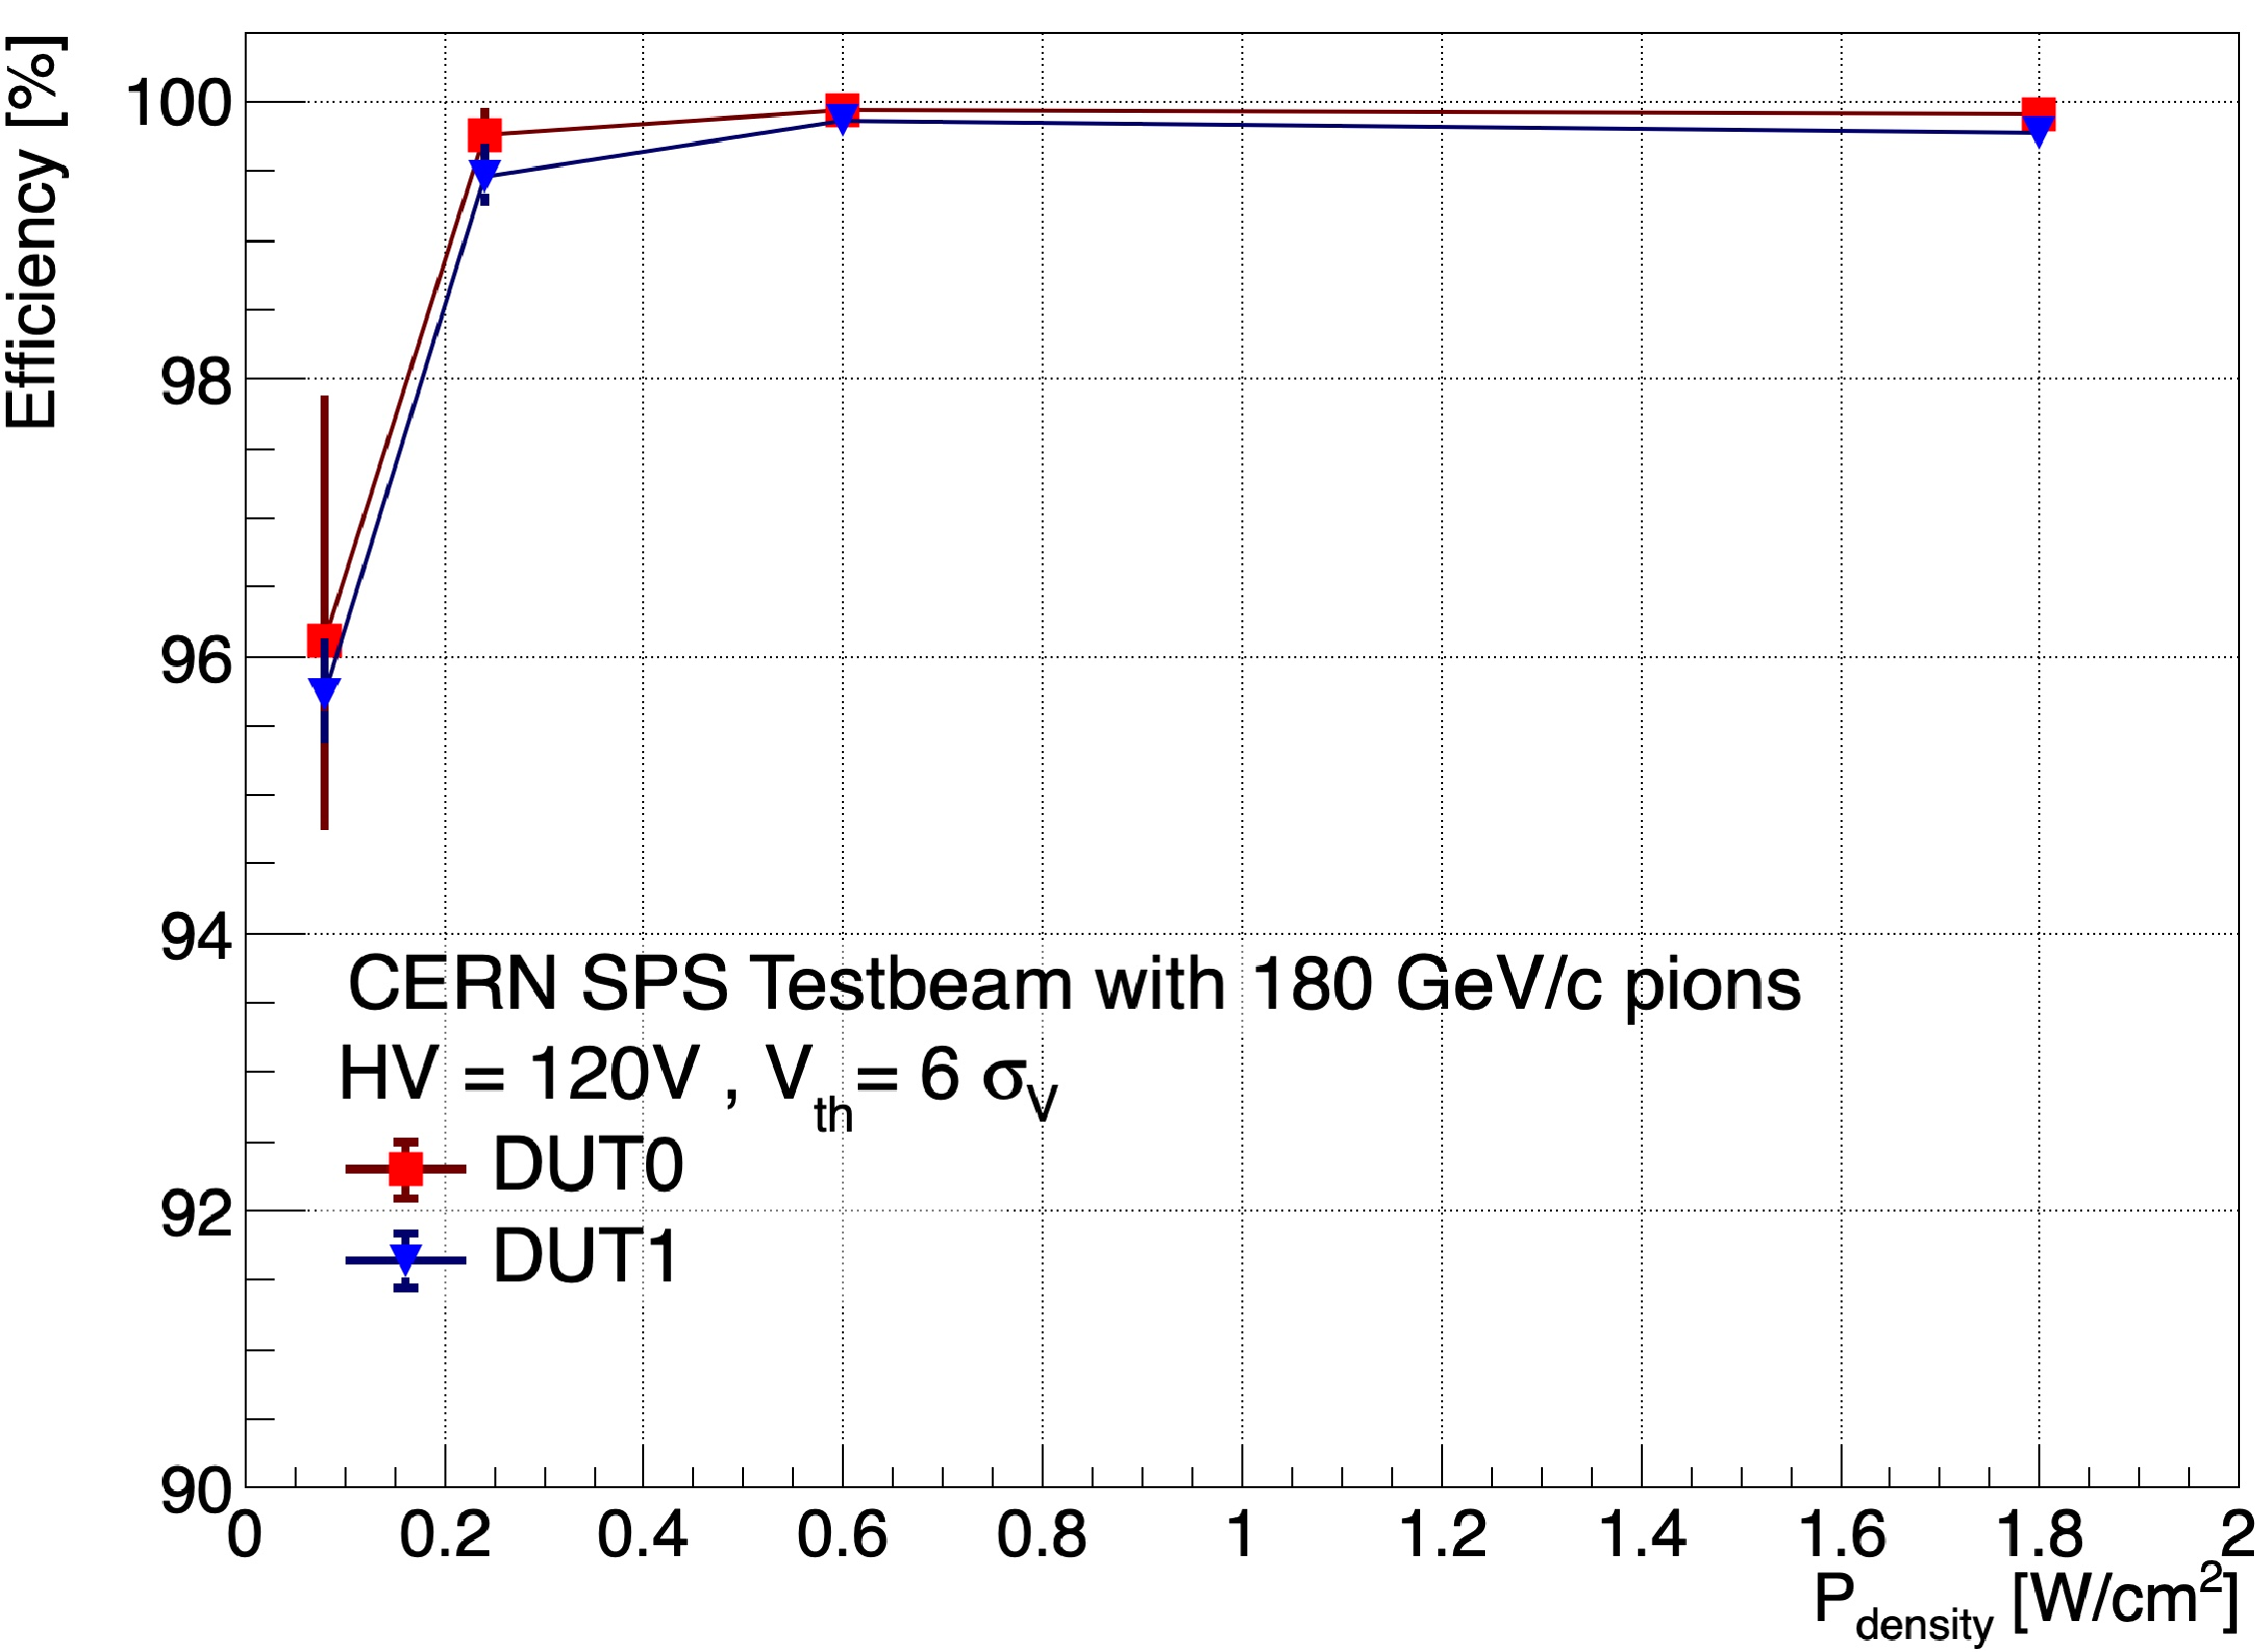
\includegraphics[width=0.65\linewidth]{files/ATTRACT_paper/eff_vs_power}
			\caption{Efficiency vs. \power for $ HV =$ \SI{120}{\volt}, evaluated in the triangular inter-pixel zone for  DUT0 (in red) and DUT1 (in blue).}
			\label{im:ATTRACT_effipreampscan} 
		\end{figure}

		Figure~\ref{im:ATTRACT_effipreampscan} and Table \ref{tab:ATTRACT_efftable} show the efficiency obtained within the triangular area for the four power density working points at a discrimination threshold of 6\noise and at a sensor bias voltage of \SI{120}{\volt}. The efficiency follows the trend expected from the ENC measurement of Table~\ref{tab:ATTRACT_gaintable}. All the power density working points show an efficiency well above 99\% except for the one at \SI{0.08}{\watt/\centi\meter^2}. At this power density a larger depletion depth would be required to operate the frontend at even higher efficiency. It is also noted that DUT0 shows a lower efficiency, compatibly with the larger ENC measured with the \Cd source (\note{section ref}). At higher power densities DUT0 is slightly more efficient than DUT1. To investigate this difference, the efficiency as a function of the discrimination threshold was inspected. The results are reported in Figure \ref{im:ATTRACT_effthrscan} for $ HV =$ \SI{120}{\volt}. The threshold scan indicates a clear difference in performance, in spite of the fact that both DUTs reach the efficiency plateau at a threshold of six standard deviations of the noise. 

		\begin{figure}[h]
			\centering 
			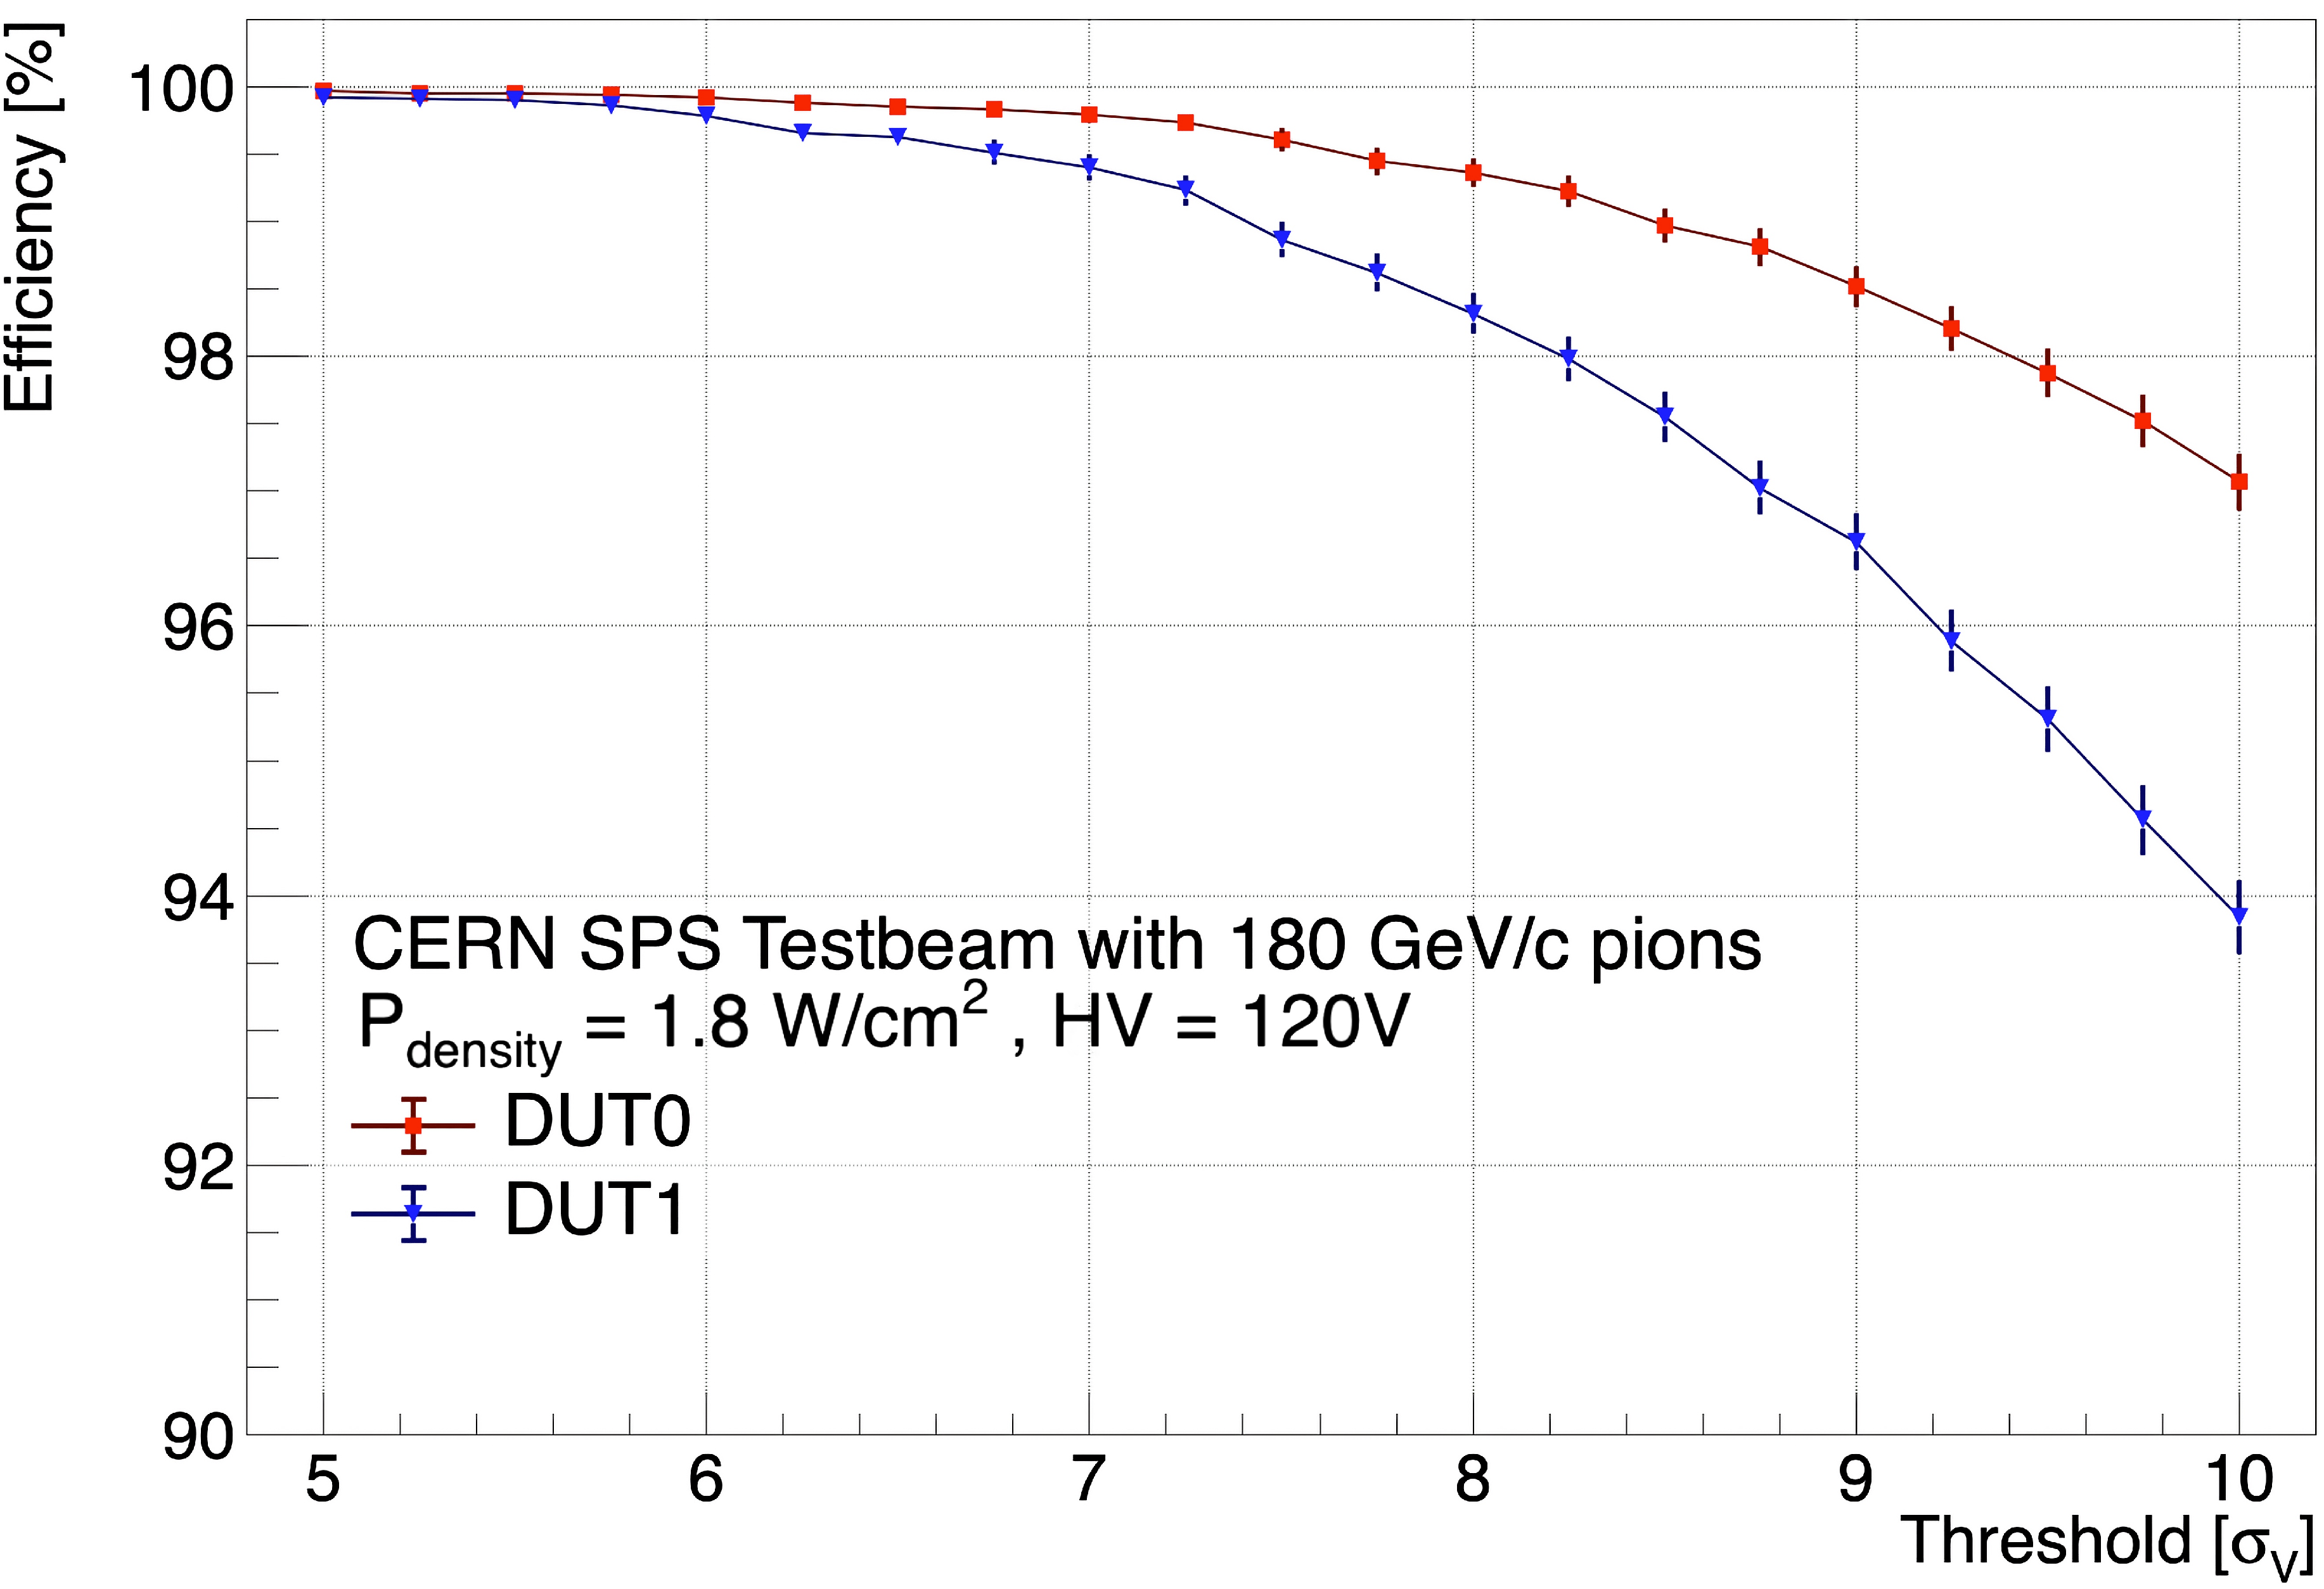
\includegraphics[width=0.65\linewidth]{files/ATTRACT_paper/EfficiencyScan_120V_150uA}
			\caption{Efficiency vs. discrimination threshold measured within the triangular inter-pixel zone for  DUT0 (in red) and DUT1 (in blue).}
			\label{im:ATTRACT_effthrscan} 
		\end{figure}

		The efficiency measurement of a sensor HV scan carried out for the working point  \power = \SI{1.8}{\watt/\centi\meter^2} is reported in Figure~\ref{im:ATTRACT_effHVscan} and Table~\ref{tab:ATTRACT_efftablehv}. 
		The scan shows that the two DUTs are in the efficiency plateau at \SI{120}{\volt}. At the \SI{50}{\ohm\cm} substrate resistivity of this prototype, increasing the HV from \SI{120}{\volt} to \SI{160}{\volt} increases the depletion depth by 15\%, which has little or no contribution for the working point at the highest power density, but could have been beneficial for the frontend operation at \SI{0.08}{\watt/\centi\meter^2} for which a small drop in efficiency was observed (Figure~\ref{im:ATTRACT_effipreampscan}).
		
		\begin{figure}[h]
			\centering 
			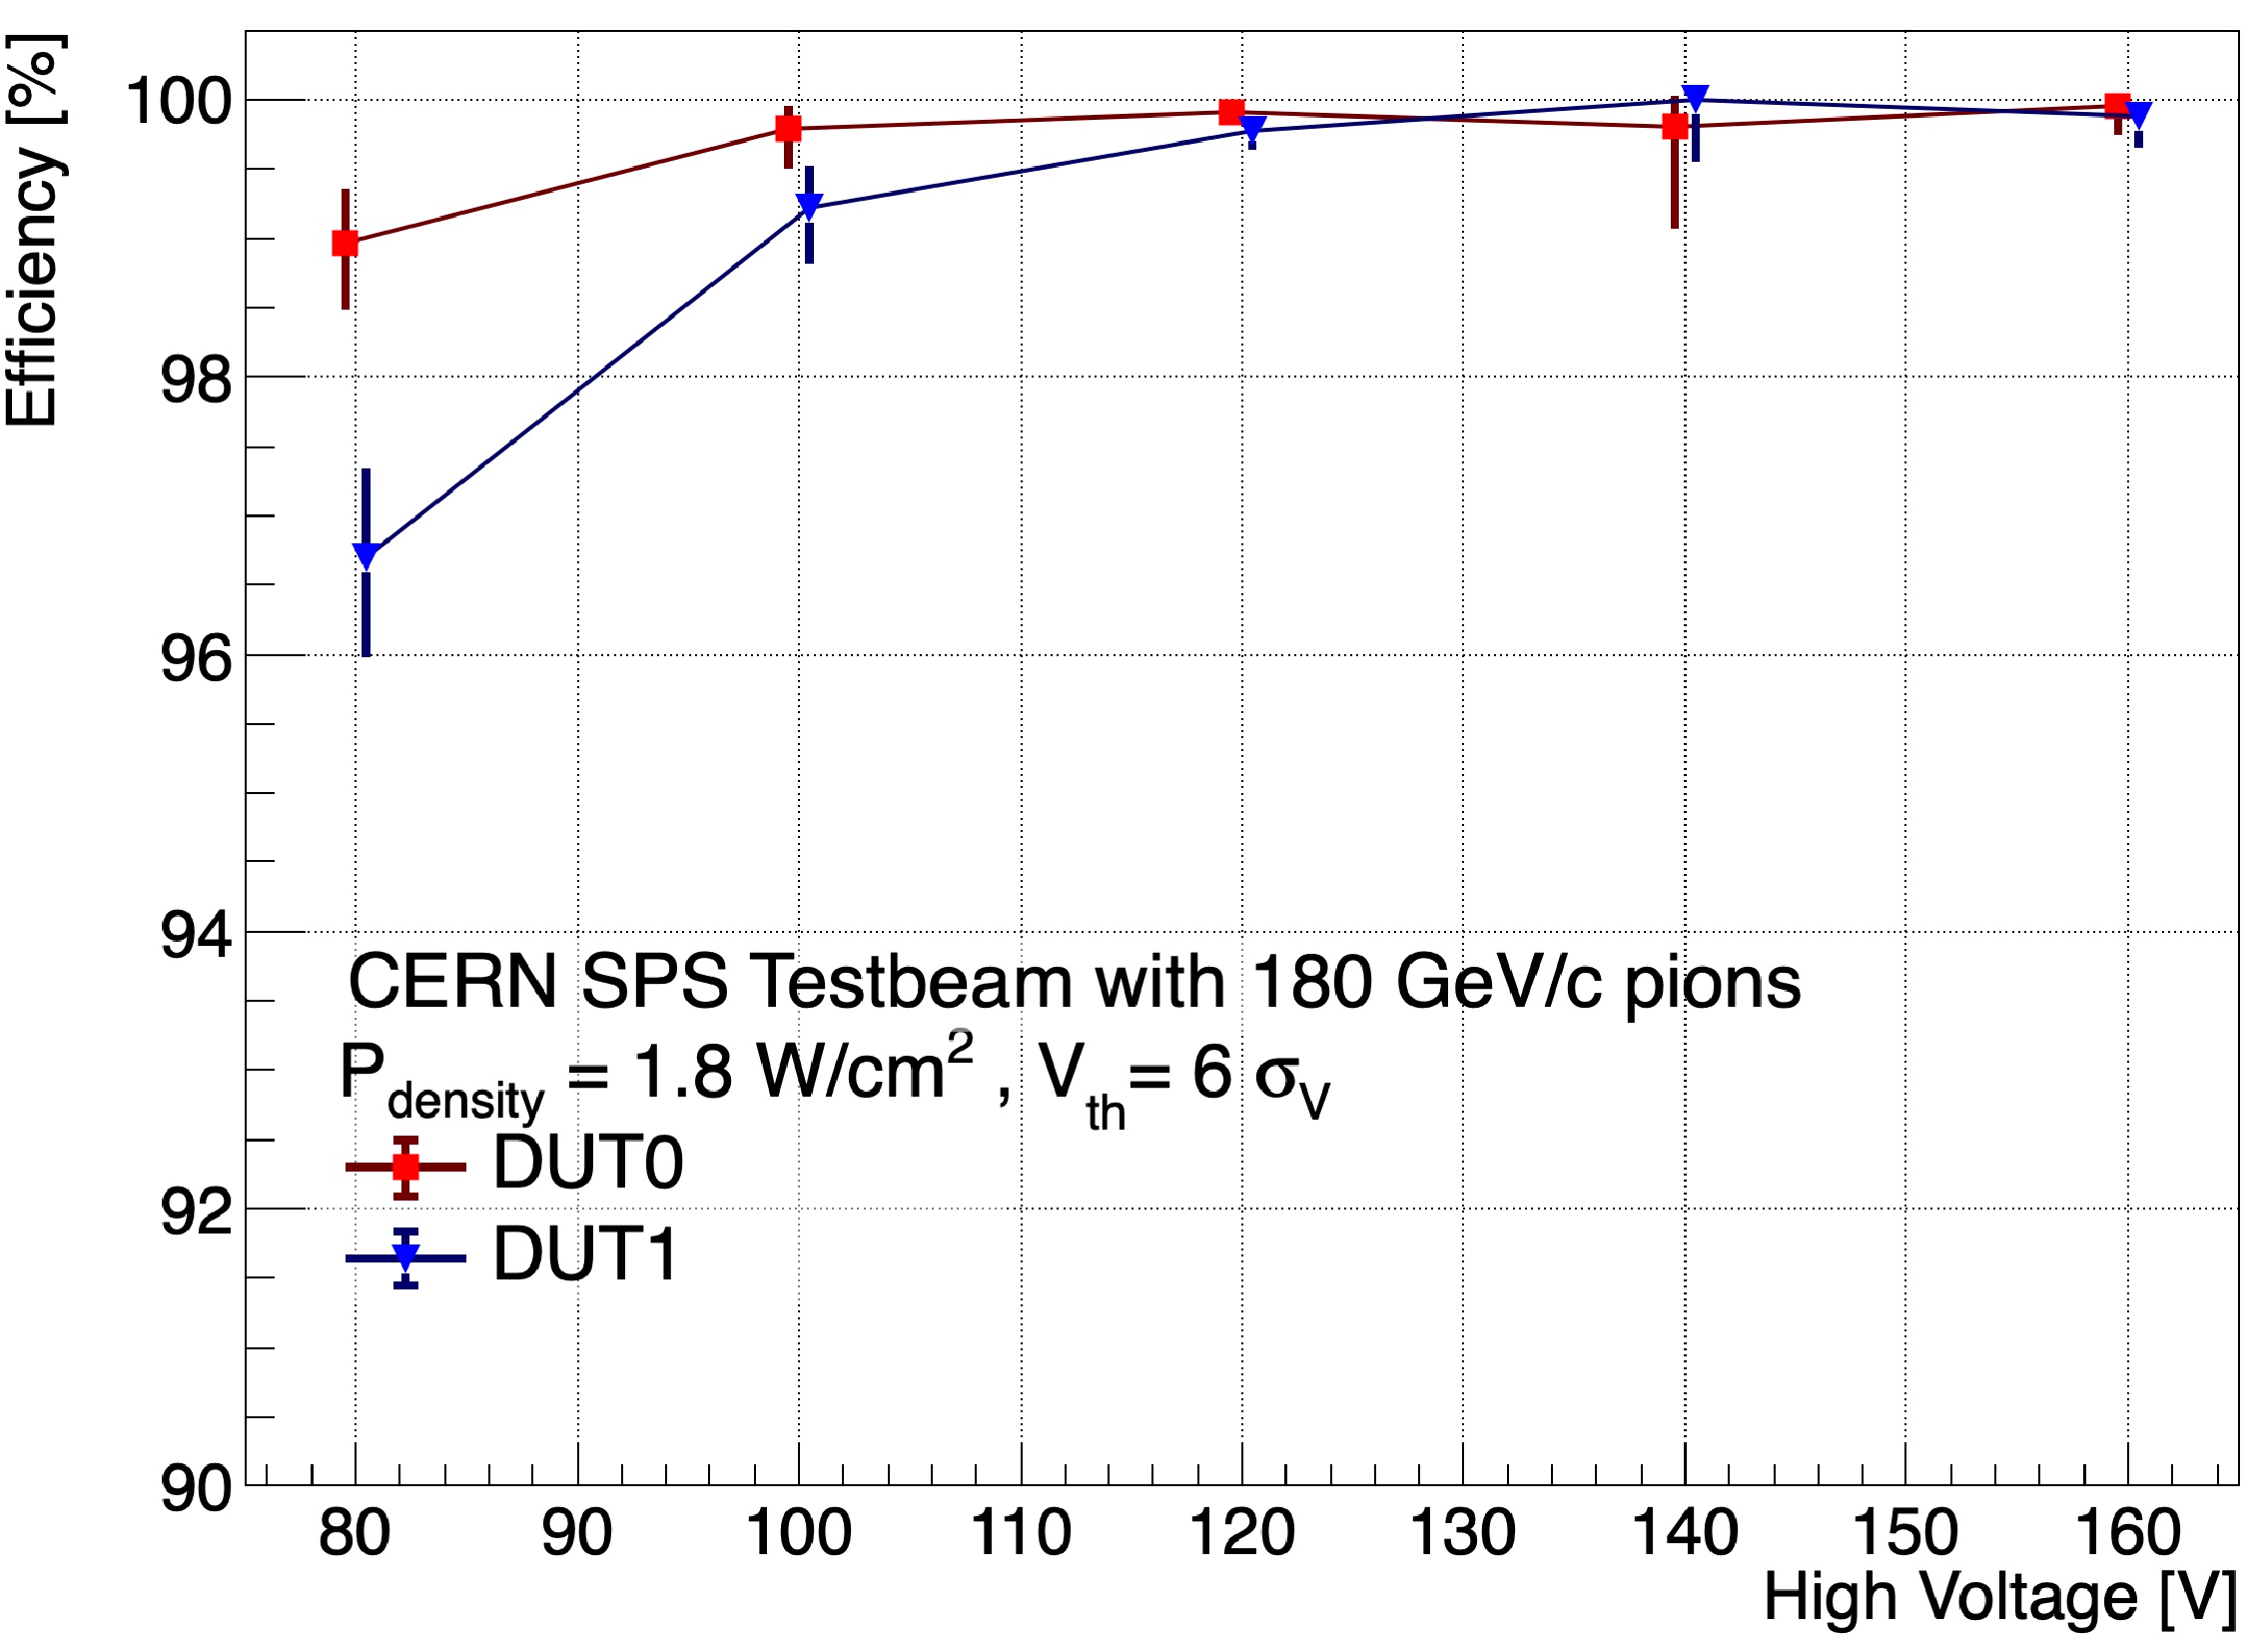
\includegraphics[width=0.75\linewidth]{files/ATTRACT_paper/eff_vs_HV}
			\caption{Efficiency vs. \!\!sensor bias voltage for the two DUTs at \power = \SI{1.8}{\watt/\centi\meter^2} and voltage threshold of 6\noise. The vertical error bars show the statistical uncertainties.}
			\label{im:ATTRACT_effHVscan}
		\end{figure}
		
		\begin{table}[h]
			\centering
			\renewcommand{\arraystretch}{1.3}
			\begin{tabular}{c|ccccc|l}
				\cline{1-6}
				\multicolumn{6}{|c|}{Efficiency measured at \power = \SI{1.8}{\watt/\centi\meter^2}}                                                                                                                         & \multicolumn{1}{c}{\textbf{}} \\ \cline{1-6}
				\multicolumn{1}{|c|}{HV [V]} & \multicolumn{1}{c|}{80} & \multicolumn{1}{c|}{100} & \multicolumn{1}{c|}{120} &\multicolumn{1}{c|}{140} & 160 &                               \\ \cline{1-6}
				\multicolumn{1}{|c|}{Efficiency DUT0 {[}\%{]}} & \multicolumn{1}{c|}{$ 98.97_{-0.46}^{+0.35} $} & \multicolumn{1}{c|}{$ 99.78_{-0.26}^{+0.14} $} & \multicolumn{1}{c|}{$ 99.91_{-0.08}^{+0.05} $} &\multicolumn{1}{c|}{$ 99.81_{-0.71}^{+0.18} $} & $ 99.95_{-0.18}^{+0.04} $ &                               \\ \cline{1-6}
				\multicolumn{1}{|c|}{Efficiency DUT1 {[}\%{]}} & \multicolumn{1}{c|}{$ 96.70_{-0.70}^{+0.61} $} & \multicolumn{1}{c|}{$ 99.21_{-0.37}^{+0.28} $}   & \multicolumn{1}{c|}{$ 99.78_{-0.11}^{+0.08} $} &\multicolumn{1}{c|}{$ 100._{-0.42}^{+0.00} $} & $ 99.88_{-0.20}^{+0.09} $ &                               \\ \cline{1-6}
			\end{tabular}
			\caption{Efficiency at different HV values for the two DUTs for \power = 1.8 W/cm$^2$. The efficiency is measured according to the definition given in the text. The uncertainties are statistical only.}
			\label{tab:ATTRACT_efftablehv}
		\end{table}


		\subsection{Time resolution measurement}
		For the time resolution measurement, the pixels OA0 of the two DUTs were carefully aligned with respect to the beamline and events in which the two pixels registered signals with amplitudes above a discrimination threshold of $ 6$ \noise in coincidence were selected. Furthermore, the telescope-track quality selection described in Section \note{section ref} and the cross-talk selection described in Section \note{insert ref here} were applied. To avoid biasing the sample with a geometrical selection, no requirement on the telescope-track position was imposed.



		\subsubsection{Time-walk correction} 
		Figure \ref{im:ATTRACT_TWcorr} shows the difference in the Time-Of-Arrival measured in pixels OA0 of  DUT0 (TOA0) and DUT1 (TOA1) as a function of the inverse of the signal amplitude in DUT0 (left) and DUT1 (right) for the working point at \SI{1.8}{\watt/\centi\meter^2} and $ HV =$ \SI{160}{\volt}. The data show a large variation of the average of the difference  TOA0$-$TOA1  as a function of the signal amplitudes, of the order of a few hundreds ps, that was corrected in the following way. 
	
		The data were divided in variable-size bins of the inverse of the amplitude containing at least 200 entries. For each of these bins for DUT0 in Figure \ref{im:ATTRACT_TWcorr} left, the most probable value of TOA0$-$TOA1 was obtained by a Gaussian fit (red points in the figure). That value was associated to the average value of the inverse of the DUT0 amplitude distribution within that bin (instead than to the center of the bin). An event-by-event correction was then applied to the inverse of the amplitude of the  signal in DUT0, using the value provided by the linear interpolation (red segments in the figure) of the two adjacent time-walk correction points.
		
		Once DUT0 was time-walk corrected in this way, the entire procedure was repeated for DUT1 (shown in Figure \ref{im:ATTRACT_TWcorr} right) to complete the time-walk correction. Given its importance for this measurement, the time-walk correction was performed also with an unbinned maximum-likelihood fit. This second method was used for a simultaneous extraction of the resolution parameter $\sigma_{TOA0-TOA1}$ and of the two time-walk correction functions for DUT0 and DUT1. For all the data samples analysed, the results were within few percent from those obtained by the method described in the text.
		\begin{figure}[h]
			\centering %
			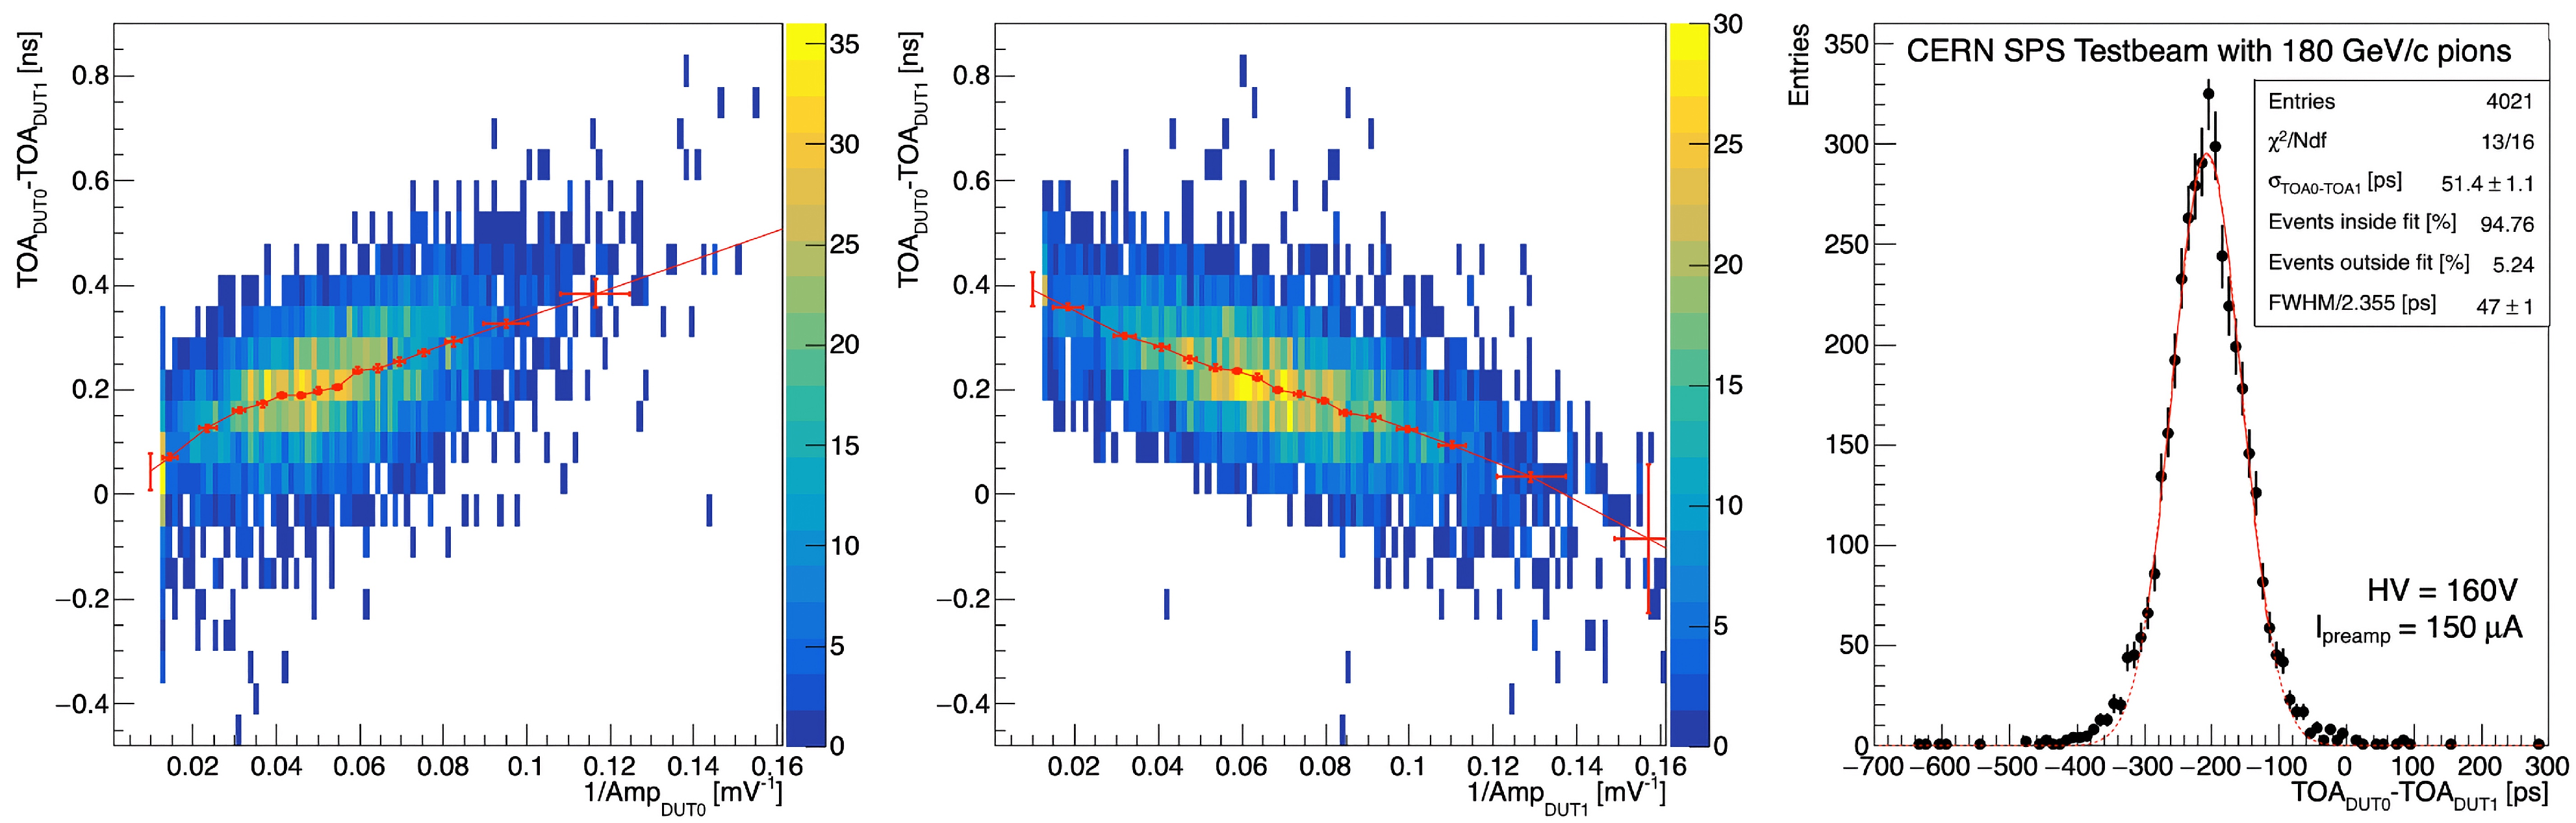
\includegraphics[width=0.92\linewidth]{files/ATTRACT_paper/TimeRes_WP7_160V}
			\caption{Distributions of the difference in TOA between the two DUTs vs. the inverse of the amplitude used for the time-walk correction of DUT0 (left) and DUT1 (right). Both DUTs were operated at \power = \SI{1.8}{\watt/\centi\meter^2} and $ HV =$ \SI{160}{\volt}. The time-walk correction points (in red) were obtained by a Gaussian fit on each bin of the inverse of the amplitude. The red segments show the linear interpolation between the time-walk correction points used to correct the data. The TOA difference contains an arbitrary offset that is irrelevant for the measurement of the time resolution.}
			\label{im:ATTRACT_TWcorr}
		\end{figure}

		\subsubsection{Extraction of the time resolution}
		Once data were corrected for time walk, Gaussian fits were performed to the TOA0$-$TOA1 distributions, including only bins containing more than 25\% of the entries at the maximum of the distribution. It was then assumed that the two DUTs have the same resolution, so that the time resolution of each DUT can be estimated as $\sigma_{t} = \sigma\_{\it TOA0-TOA1}/\sqrt{2}$.

		As an example, Figure \ref{im:ATTRACT_TOF} shows the resulting TOA difference distribution after time-walk correction for the data acquired at the working points \SI{1.8}{\watt/\centi\meter^2} and $ HV =$ \SI{160}{\volt} (left) and \SI{0.08}{\watt/\centi\meter^2} and 120 V (right).  In the case of the former, that is the best working point for time resolution, the standard deviation obtained by the Gaussian fit is measured to be $\sigma_{TOA0-TOA1}=(51.4 \pm 1.1)$ ps. 
		Therefore the time resolution of each DUT is estimated to be
		\begin{equation}
    		\sigma_{t} = \frac{\sigma\_{\it TOA0-TOA1}}{\sqrt{2}} = (36.4 \pm 0.8) \si{\pico\second}.
		\end{equation}
		\begin{figure}[h]
			\centering %
			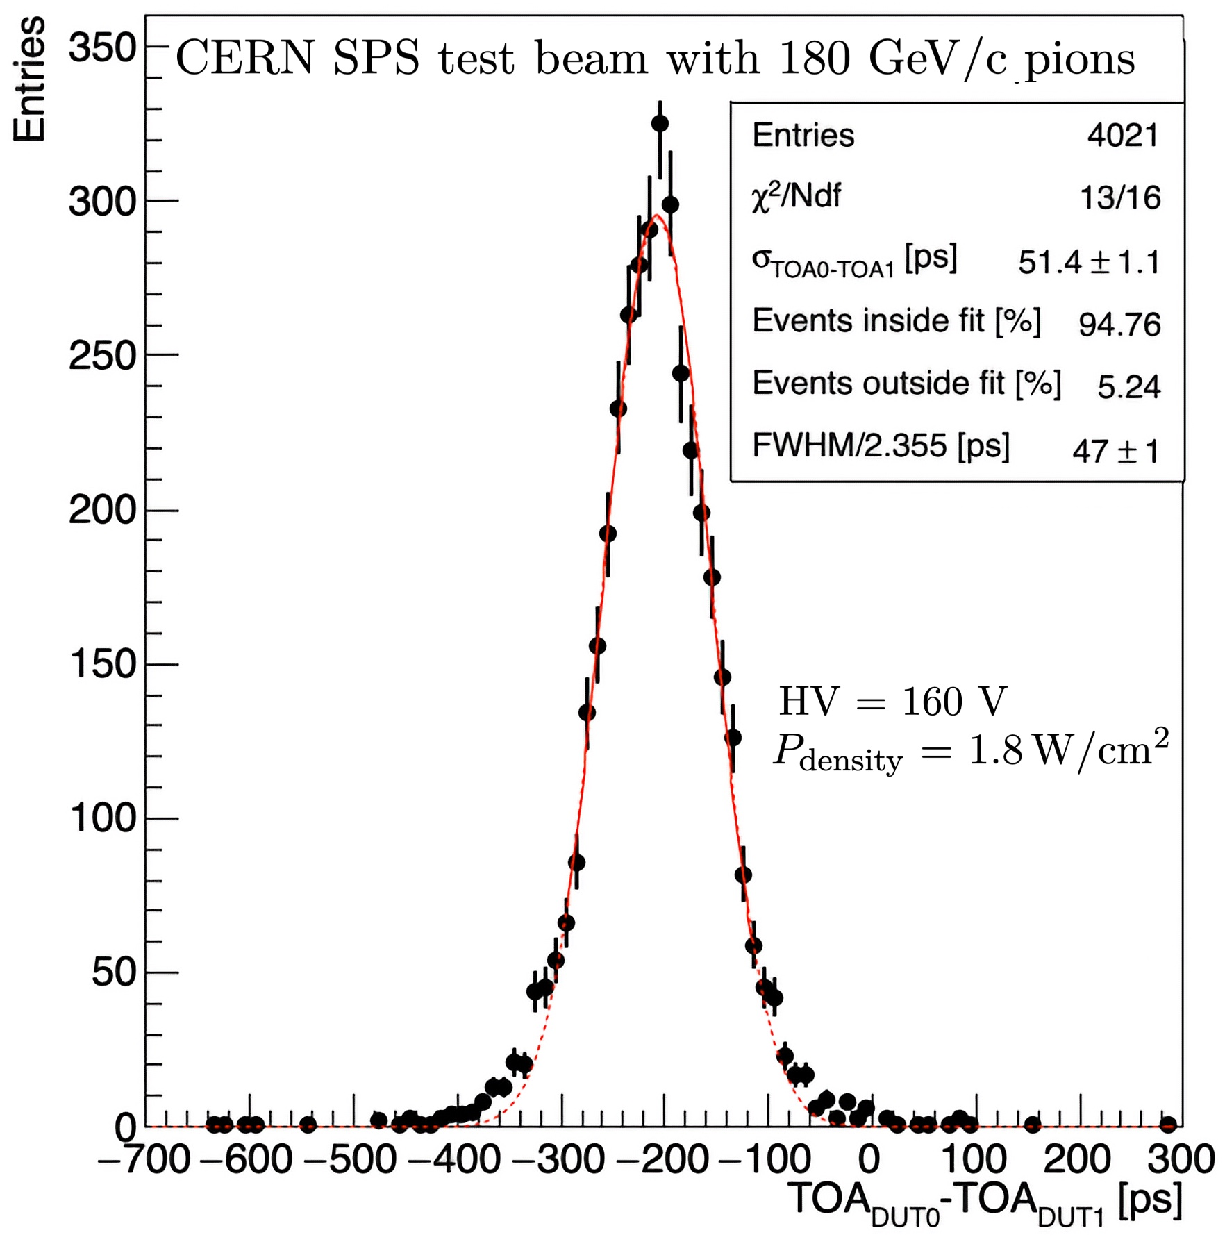
\includegraphics[width=0.47\linewidth]{files/ATTRACT_paper/TimeRes_WP7_160V_Gauss}
			\qquad
			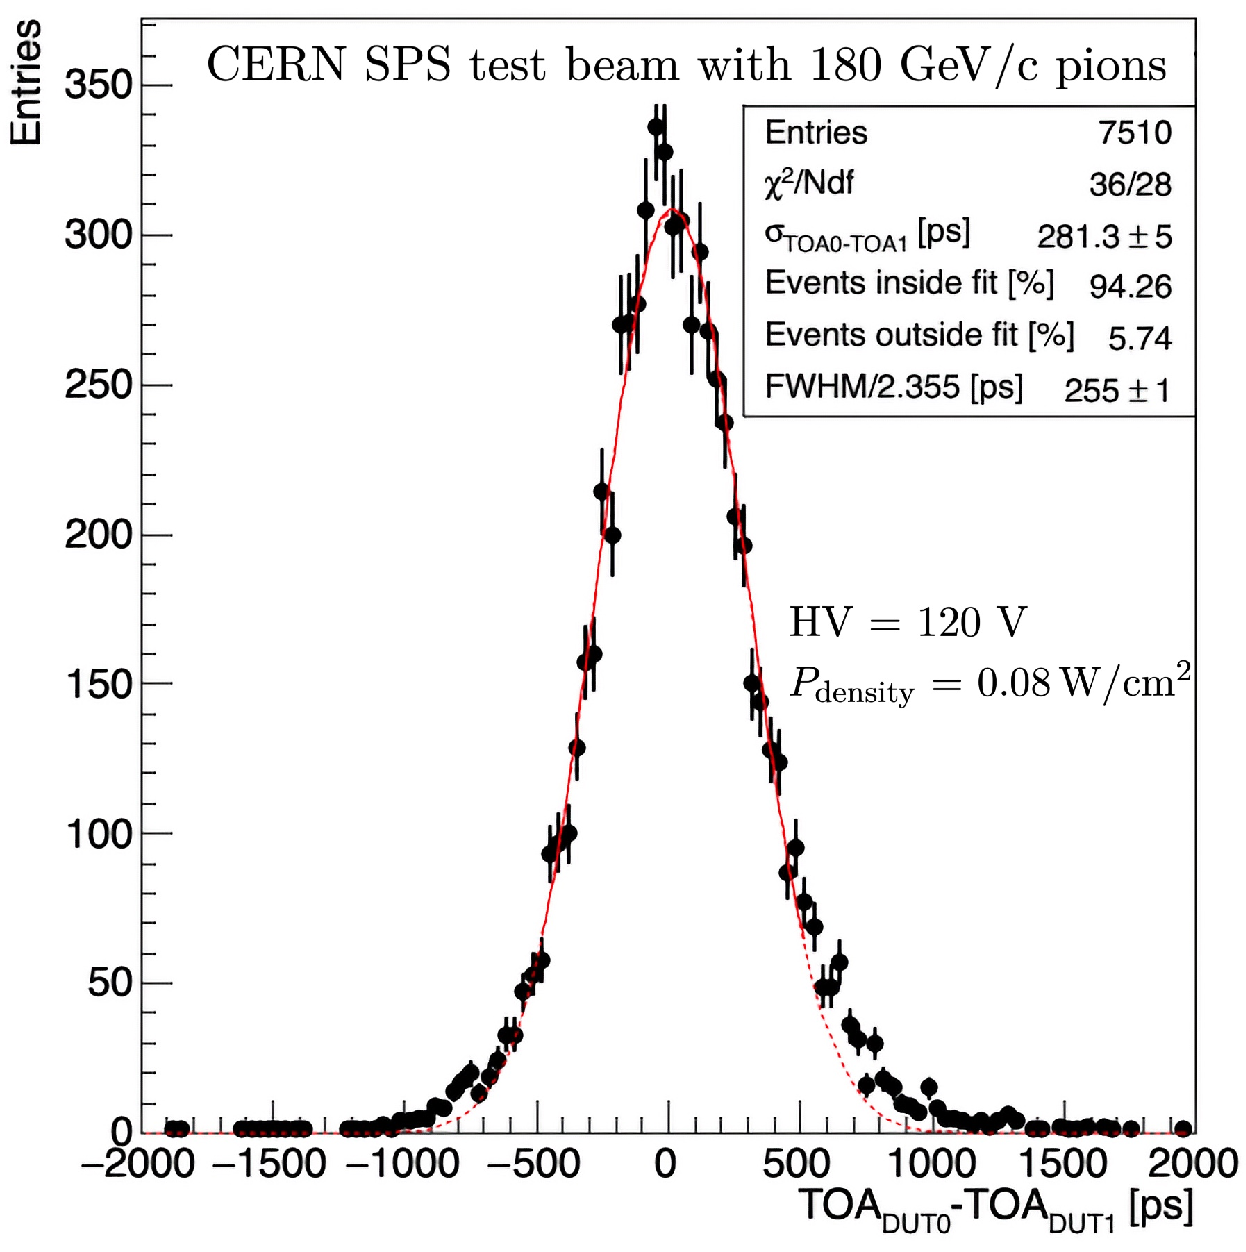
\includegraphics[width=0.47\linewidth]{files/ATTRACT_paper/TimeResolution_120V_7uA_Gauss}
			\caption{ TOA difference between pixels OA0 of DUT0 and DUT1 after time-walk correction for the two working points reported in the panels. A constant arbitrary offset is present, which is irrelevant for the time-resolution calculation. The  red lines show the results of the Gaussian fit using only the bins with more than 25\% of the entries in the maximum of the distribution. The full red lines show the ranges used for the fits, while the dashed red lines allow the estimation of the non-Gaussian components in the tails.}
			\label{im:ATTRACT_TOF}
		\end{figure}
		
		The fraction of events exceeding the Gaussian fit in the tails of the distribution of Figure \ref{fig:TOF} is approximately 5\%. This fraction of events represents the typical non-Gaussian component found in the tails of the time-resolution distribution for  all the data sets acquired at the testbeam at different sensor and preamplifier bias.
		As a consequence the resolutions quoted in the following refer to 95\% of the signals acquired by the DUTs.

		Figure \ref{im:ATTRACT_TOFHV} top shows the time resolution as a function of the HV for the highest power consumption working point   $ I_{\text{preamp}} = \SI{150}{\watt/\centi\meter^2} $.
		The time resolution varies between 60 and 36 ps with the HV between 80 and 160 V.
		At $ HV = \SI{120}{\volt} $ the timing performance is approximately 20\% worse than the one measured at 160 V.

		Figure \ref{im:ATTRACT_TOFHV} bottom shows the time resolution measured at $ HV = \SI{120}{\volt} $  for the  four $I_{\text{preamp}}$ working points. As expected, the time resolution depends on the preamplifier current. A significant degradation of the performance is observed for the lowest power-consumption working point studied $I_{\text{preamp}} = $  \SI{7}{\watt/\centi\meter^2}, for which the time resolution still remains  at the level of 200 ps.

		\vspace{5pt}
		\begin{figure}[h]
			\centering %
			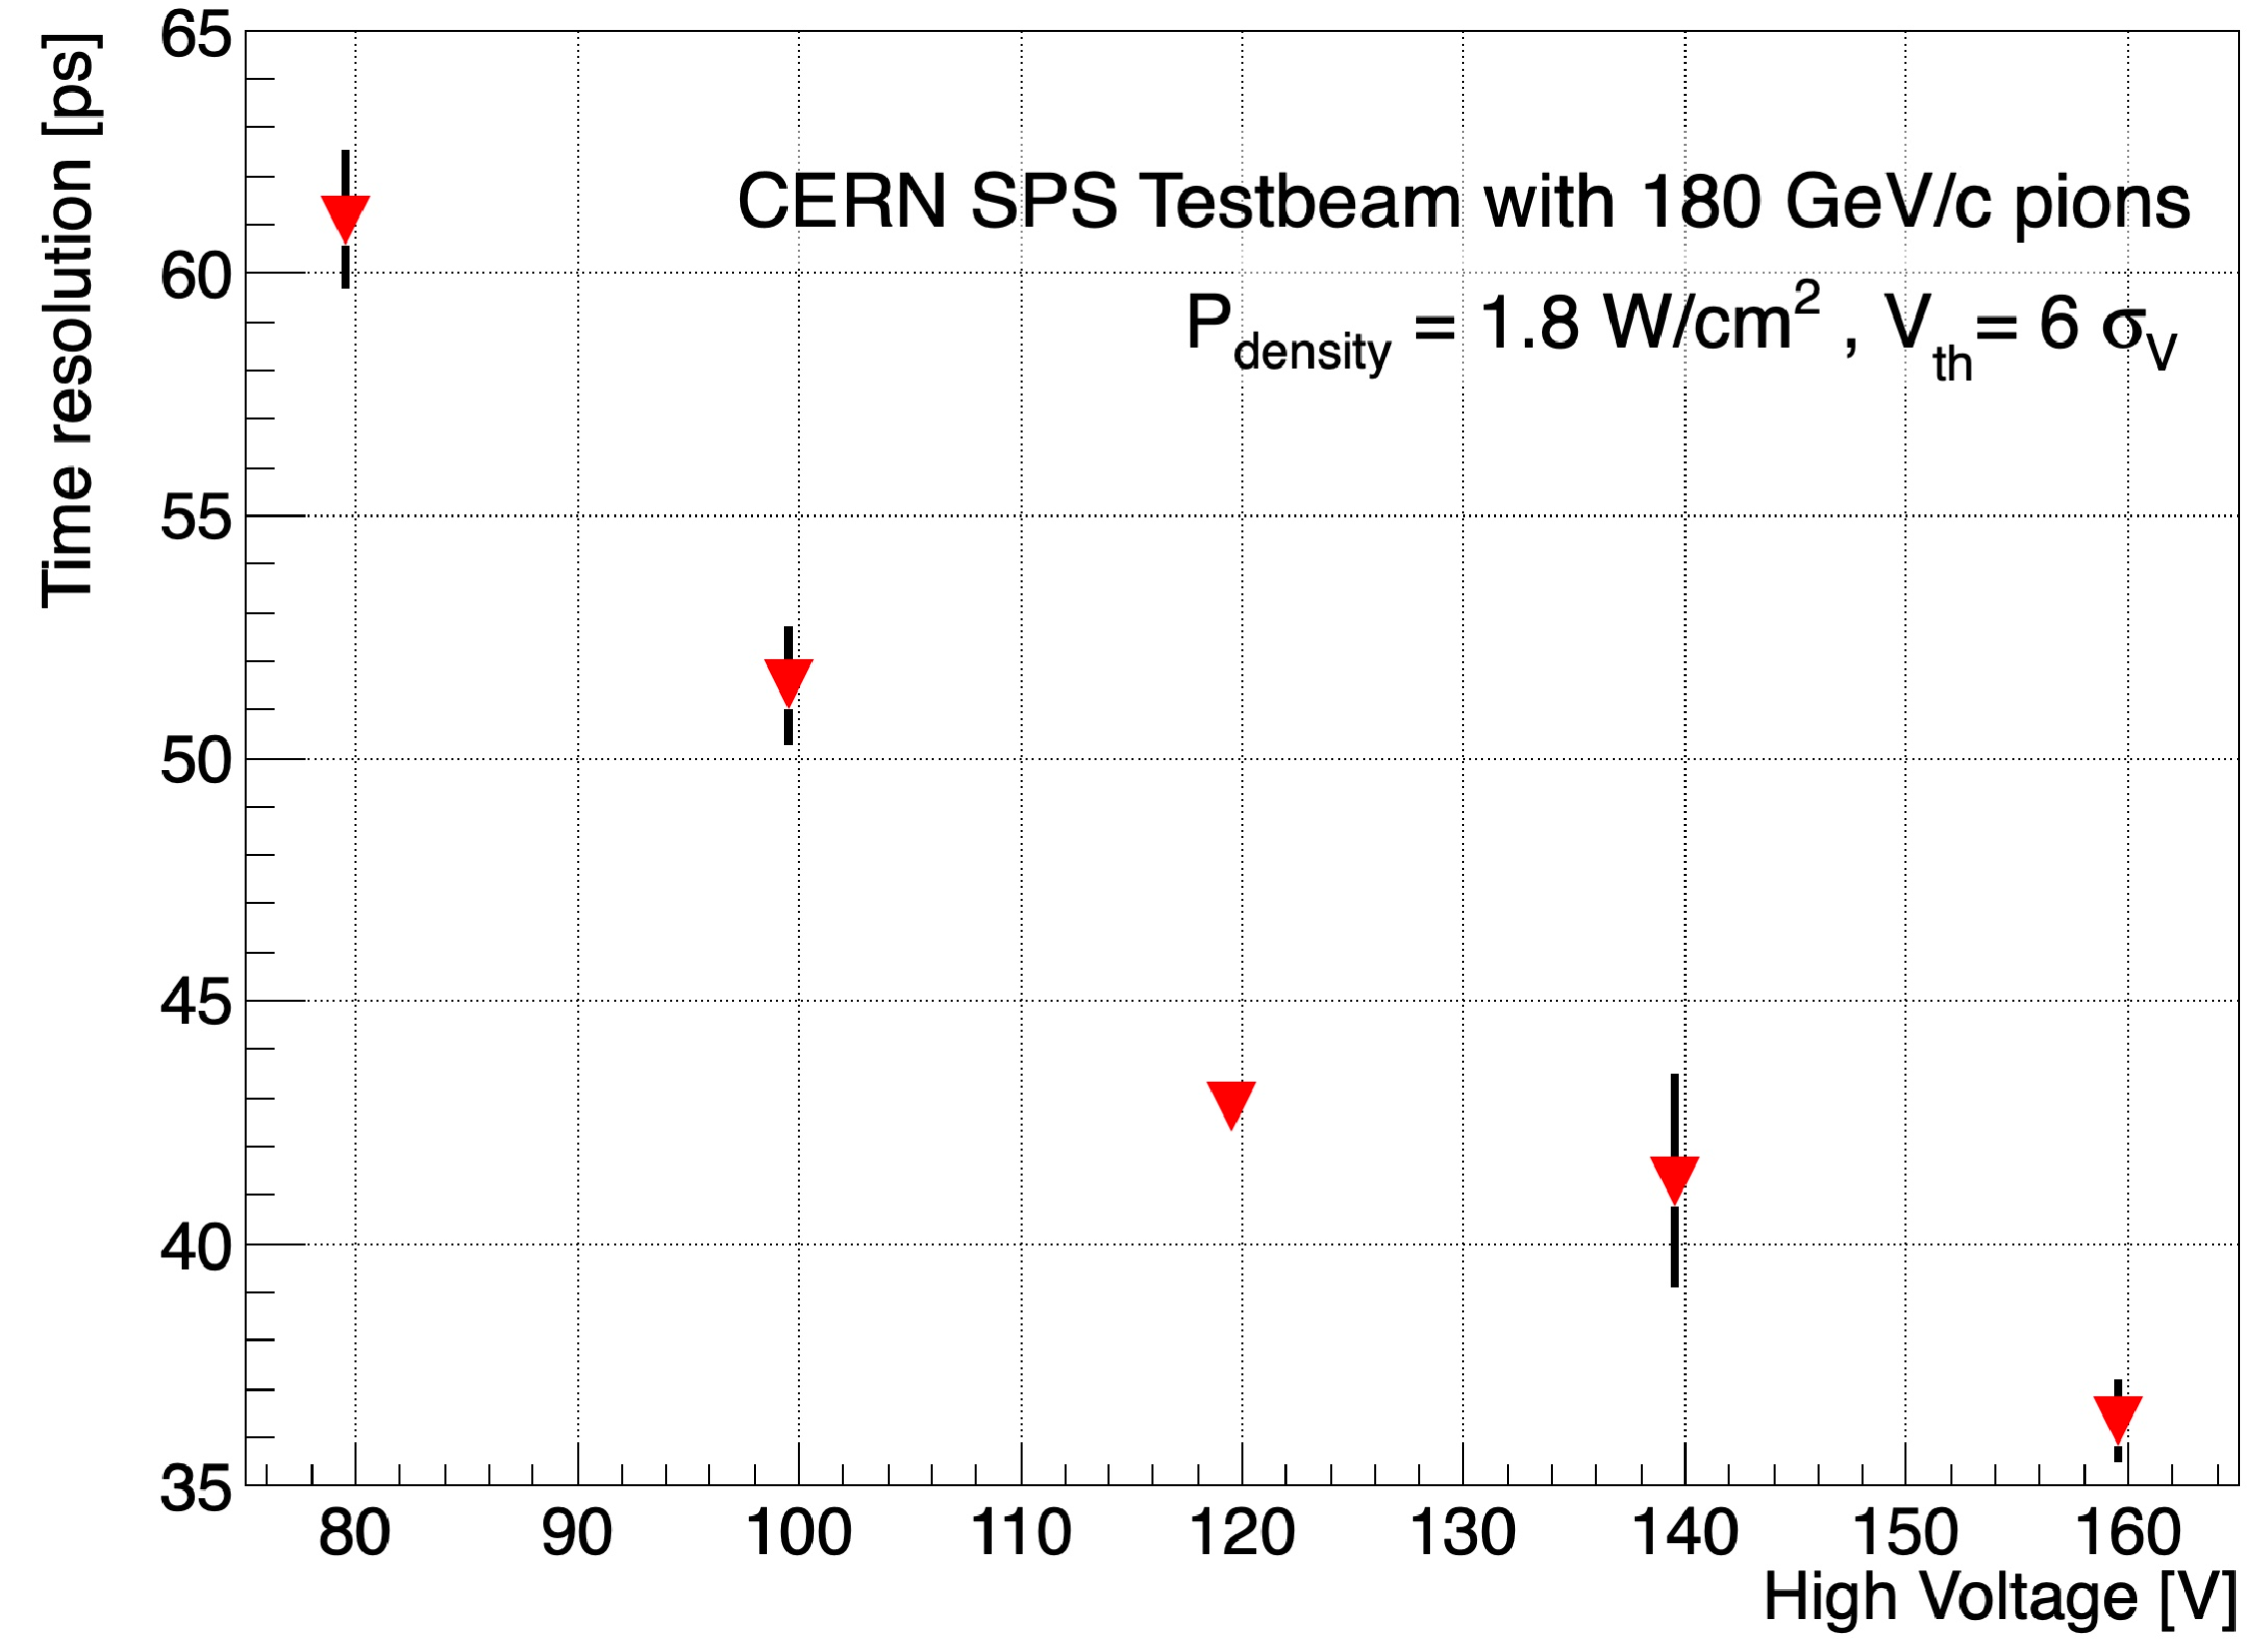
\includegraphics[width=.65\textwidth,trim=0 0 0 0, clip]{files/ATTRACT_paper/timeres_vs_HV}
			\vspace{10pt}
			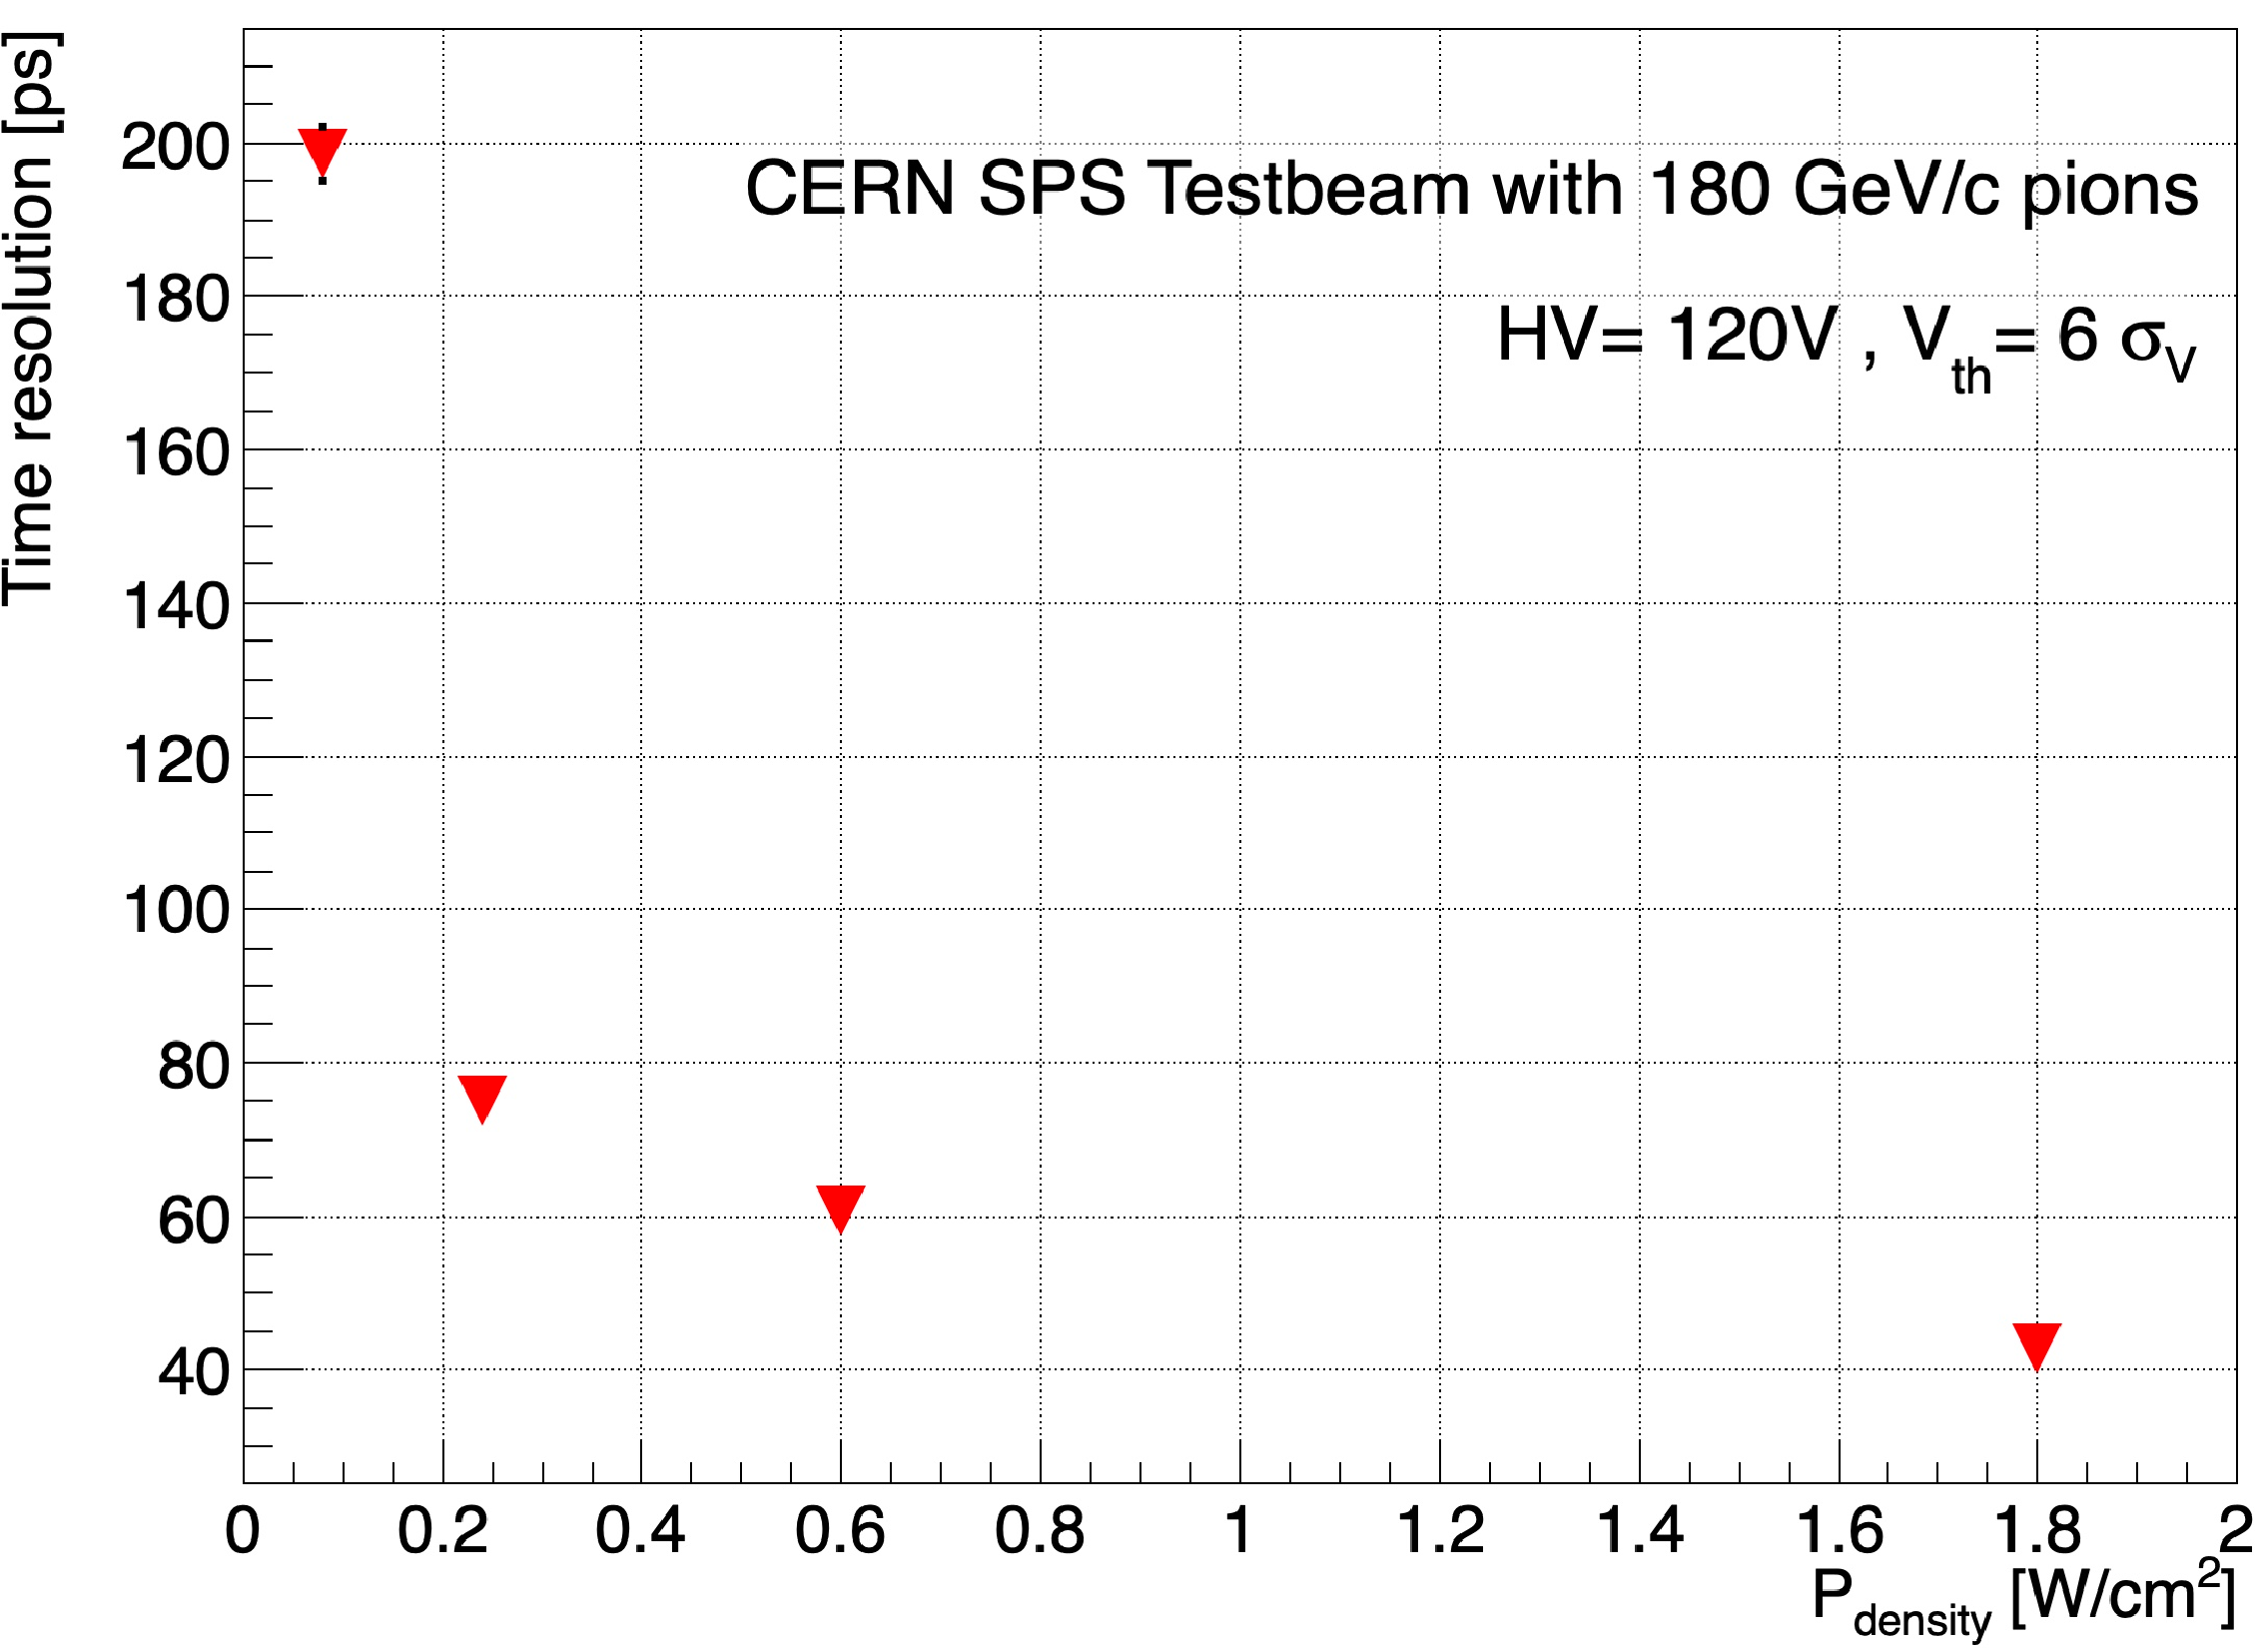
\includegraphics[width=.65\textwidth,trim=0 0 0 0, clip]{files/ATTRACT_paper/timeres_vs_power}
			\caption{Top: time resolution as a function of sensor bias voltage at $ I_{\text{preamp}} = \SI{150}{\watt/\centi\meter^2}$. Bottom: time resolution as a function of $I_{\text{preamp}} $ for sensor bias voltage $HV = $ 120 $V$. The time resolution is defined as $(\sigma\_{\it TOA0-TOA1})/\sqrt{2}$. It refers to the Gaussian component of the data, which is approximately 95\% of the total.}
			\label{im:ATTRACT_TOFHV} 
		\end{figure}
		
		
		
		
		
		
		
		
		
		
		
		
		
		
		
		
		
		
		
		
		
		
		
		
		
		
		
		
		
		
		
		
		
		
		
		
		
	\clearpage
	\section{Test Beam Characterisation of \textit{MONOLITH} Prototypes}
	In October 2022, the \textit{MONOLITH} prototype was tested during a test beam campaign organised at the CERN SPS North Area experimental hall. The beam used to qualify the ASIC was composed of pions with a momentum of \SI{120}{\giga\electronvolt}/c a beam spread of about a few millimetres wide and very straight tracks (almost no beam divergence). The track position on the DUT were reconstructed using the FE-I4 UniGe telescope \cite{telescope} and allowed for a mesure of the detection efficiency and time resolution as a function of the particle position within the pixel. Expecting better time resolution performance compared to the \textit{ATTRACT} prototypes and to extract the time resolution of a single ASIC without having to assume two identical ones, two sub-\SI{10}{\pico\second} time reference were added to the set-up.  
		
	The results are presented for the prototype as a function of the power density (\power), as a function of the High Voltage (HV) bias given to the substrate and as a function of the particle's position within the pixel. The following section refers to the work published in early 2023 in the Journal of Instrumentation (JINST) \cite{MONOLITH_proto2_20ps}.
		
		\subsection{frontend Calibrations}
		A radioactive \Fe source was used to characterise the ASIC analog electronics chain, comprising the pixel, the preamplifier and the driver, at five working points corresponding to power density values \power = 0.04, 0.13, 0.36, 0.9 and \SI{2.7}{\watt/\centi\meter^2}. The differential analog output signals were used for this measurement.
		The ENC of the frontend electronics, reported in Table~\ref{tab:MONO_gain}, was computed as 
		\begin{equation}
			ENC = \frac{\sqrt{\sigma_{\text{V}}^2 -2\sigma_{\text{scope}}^2}}{A_q}
		\end{equation}
		where \noise is the standard deviation of the electronic-noise distribution measured by the oscilloscope when the frontend is connected, $\sigma_{\text{scope}}$ is the voltage noise of the oscilloscope with the open input connector, taken twice to account since the signals used are the difference of two opposite polarities signals for the same pixel individually recorded on a separate oscilloscope channel, and $A_q$ is the charge gain.
		
		\begin{table}[h]
			\centering
			\renewcommand{\arraystretch}{1.3}
			\begin{tabular}{|c|c|c|c|c|}
			\cline{1-5}
			\cline{1-5}
			\ \power [W/cm$^2$] &  \noise [mV] & $\sigma_{\text{scope}}$ [mV] & $A_q$ [mV/fC] & ENC [electrons] \\
			\cline{1-5}
			2.7   & $ 1.45 \pm 0.02 $ & $ 0.39\pm0.01 $ & $89.4 \pm 1.1 $ & $~~93\pm2$ \\
			0.9   & $ 1.06 \pm 0.02 $ & $ 0.39\pm0.01 $ & $67.4 \pm 0.8 $ & $~~84\pm1$ \\
			0.36  & $ 0.89 \pm 0.01 $ & $ 0.39\pm0.01 $ & $45.3 \pm 0.8 $ & $~~97\pm2$ \\
			0.13  & $ 0.58 \pm 0.01 $ & $ 0.16\pm0.01 $ & $26.6 \pm 0.5 $ & $ 125\pm5$ \\
			0.04  & $ 0.67 \pm 0.01 $ & $ 0.16\pm0.01 $ & $27.0 \pm 0.5 $ & $ 145\pm8$ \\
			\cline{1-5}
			\end{tabular}
			\caption{Charge gain and ENC measured with a $^{55}$Fe source at five different values of the frontend power density. The standard deviations  of the voltage noise and of the oscilloscope noise used for the calculation of the ENC are also reported.}
			\label{tab:MONO_gain} 
		\end{table}

	
		\subsection{Testbeam Setup, Track-Selection Criteria and Data Samples}

		A pion beam of \SI{120}{\giga\electronvolt}/c momentum delivered at the CERN SPS testbeam facility was used to characterise the \textit{MONOLITH} prototype and measure its detection efficiency and time resolution. 

		The experimental setup is illustrated in Figure~\ref{im:MONO_Setup}. The device under test (DUT), wire-bonded on a dedicated PCB, was installed in the middle of the six detection planes of the UniGe FEI4 telescope for charged-particle tracking \cite{telescope}. An image of the PCB with the ASIC glued is given in Figure \ref{im:MONO_pcb}.
		\begin{figure}[h]
			\centering
			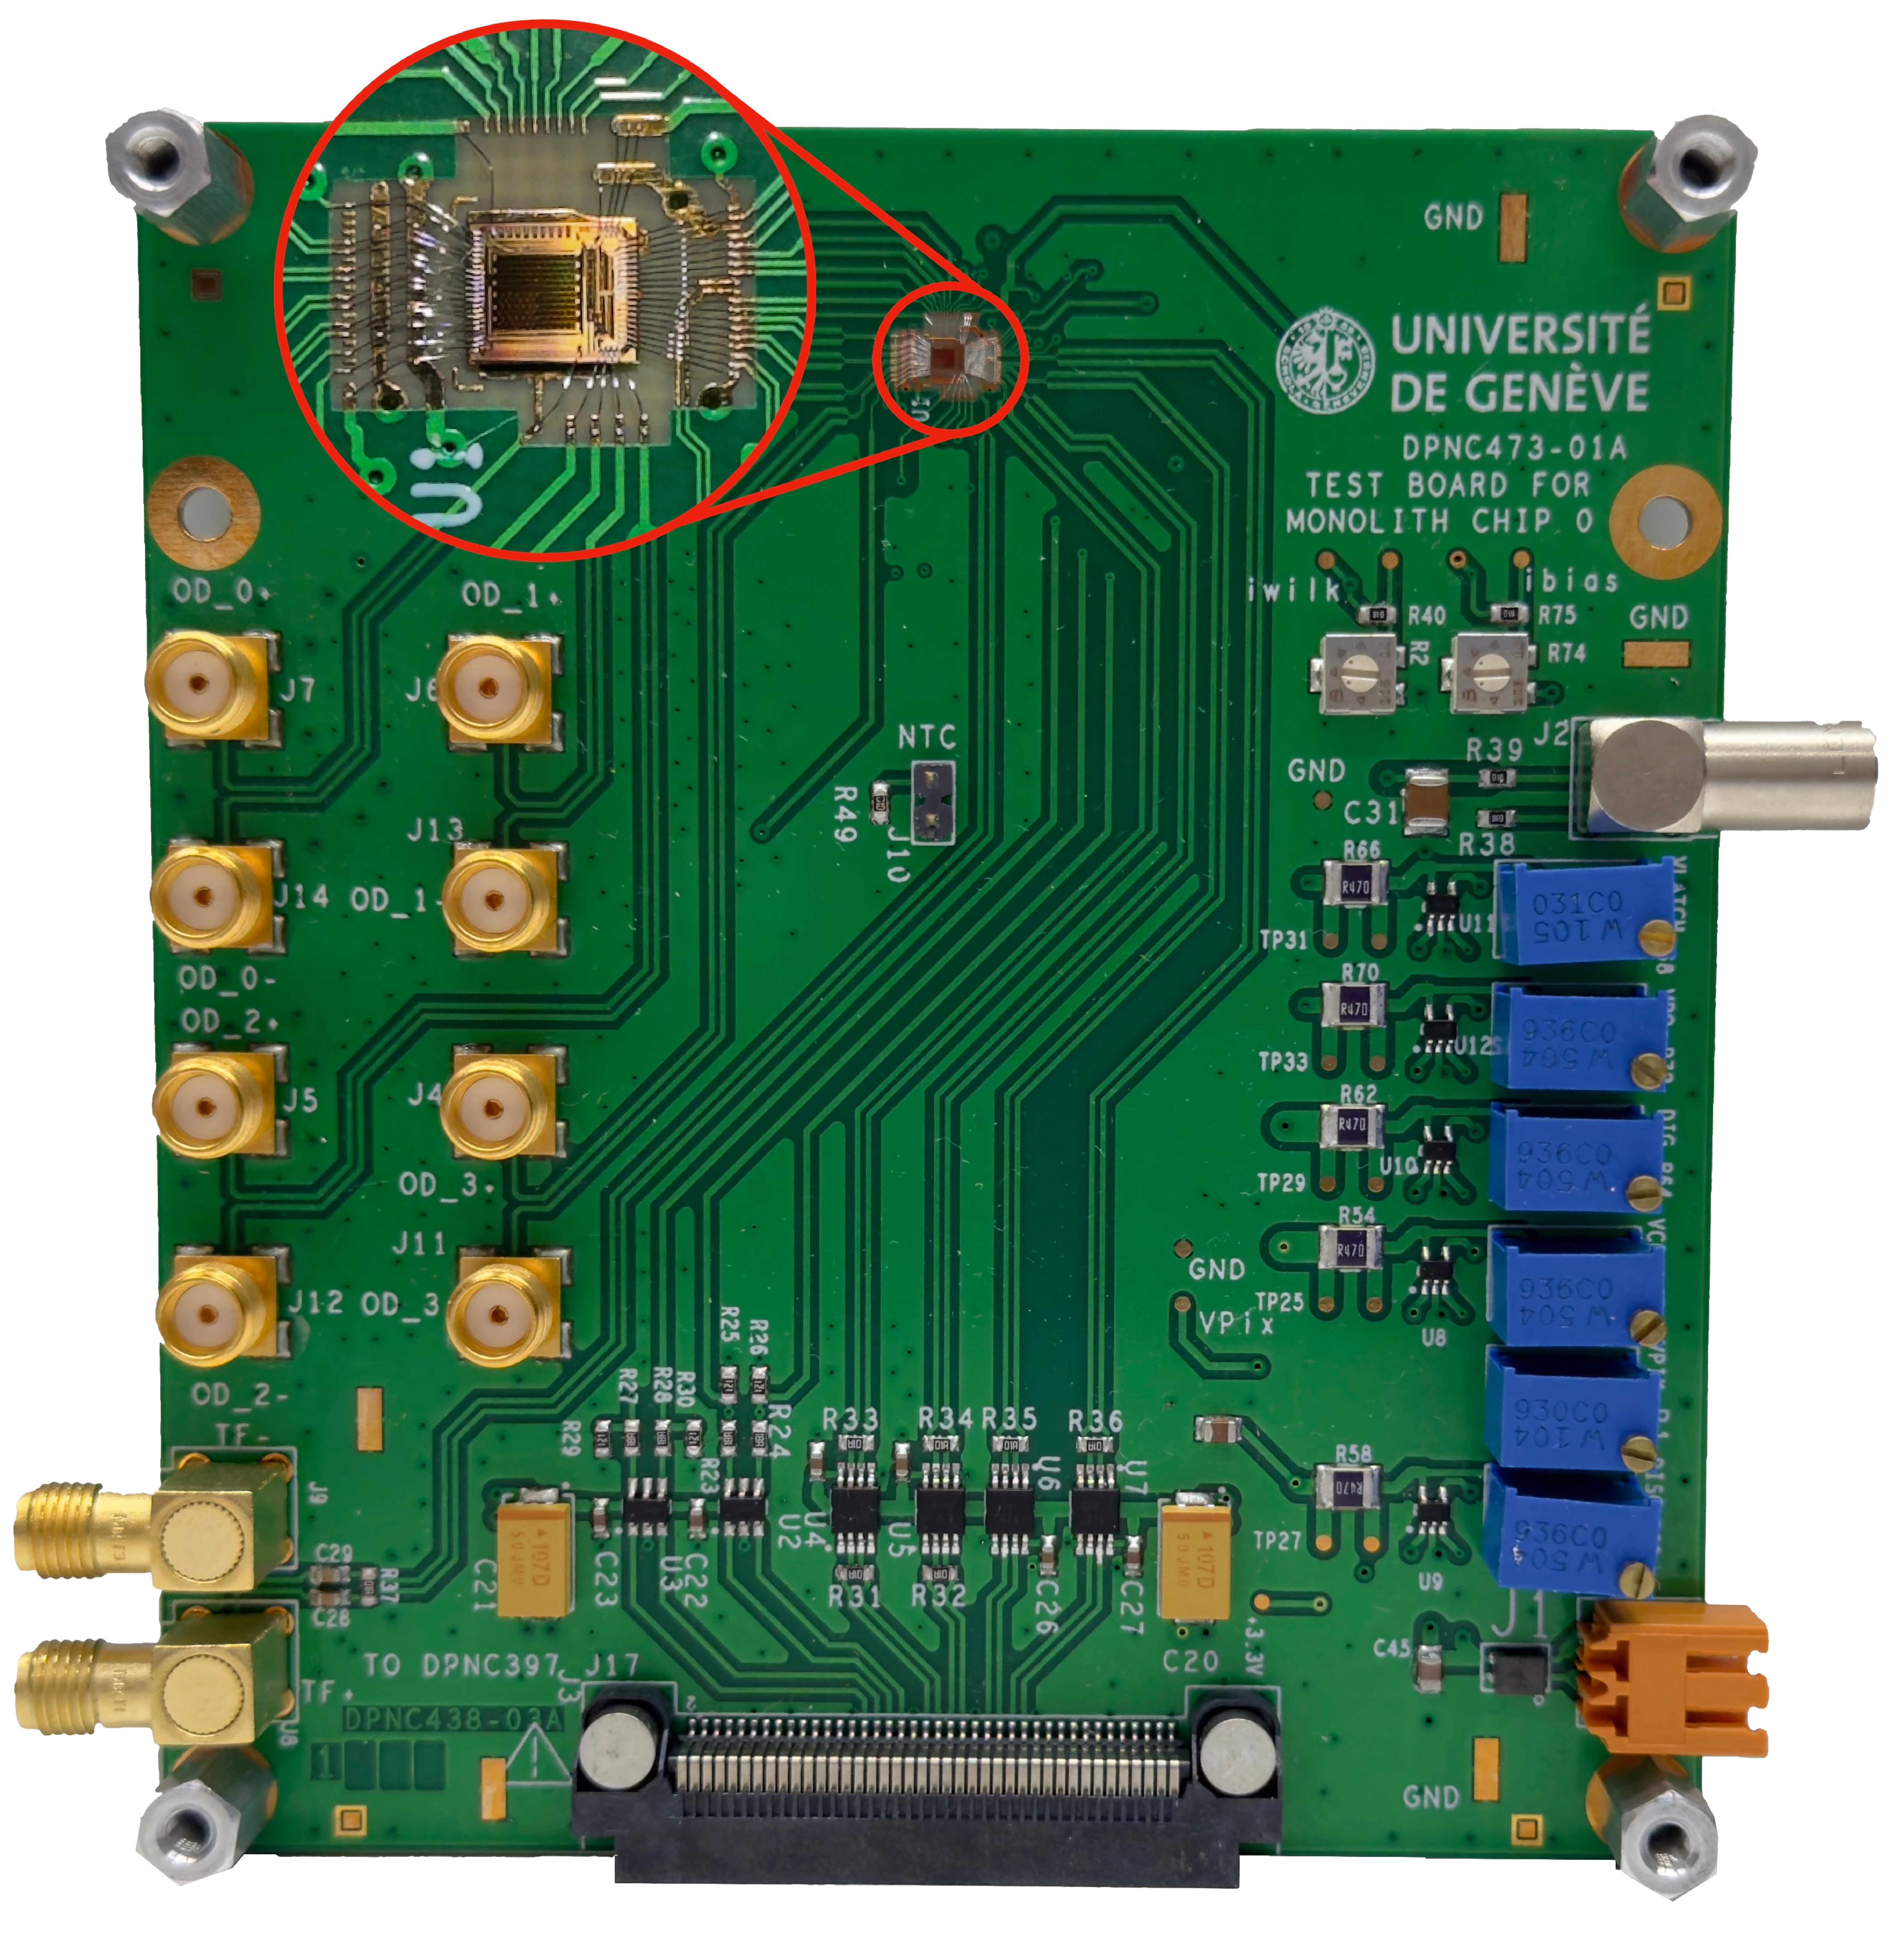
\includegraphics[width=0.7\linewidth]{files/MONOLITH_paper/pcb_mono}
			\caption{PCB used for testing the \textit{MONOLITH} prototype, which can be seen in the zoomed-in frame. The blue trimmers are used to regulate the different low voltages provided to the ASIC. The black bottom connector is the UniGe GPIO interface for digital configuration and communication. The metallic grey connector on the right provides the HV to the ASIC while the orange connector provides the master low voltage alimentation. The golden (SMA) connectors on the right are used to feed the oscilloscope the analog signals, there are two per analog pixel as both polarities are available. }
			\label{im:MONO_pcb} 
		\end{figure}
		
		 Two commercial MCP detectors, MCP0 and MCP1 hereafter, with expected time resolution for minimum-ionising particles of approximately 5 ps, were installed downstream the telescope to provide a very precise time reference.

		\begin{figure}[h]
			\centering
			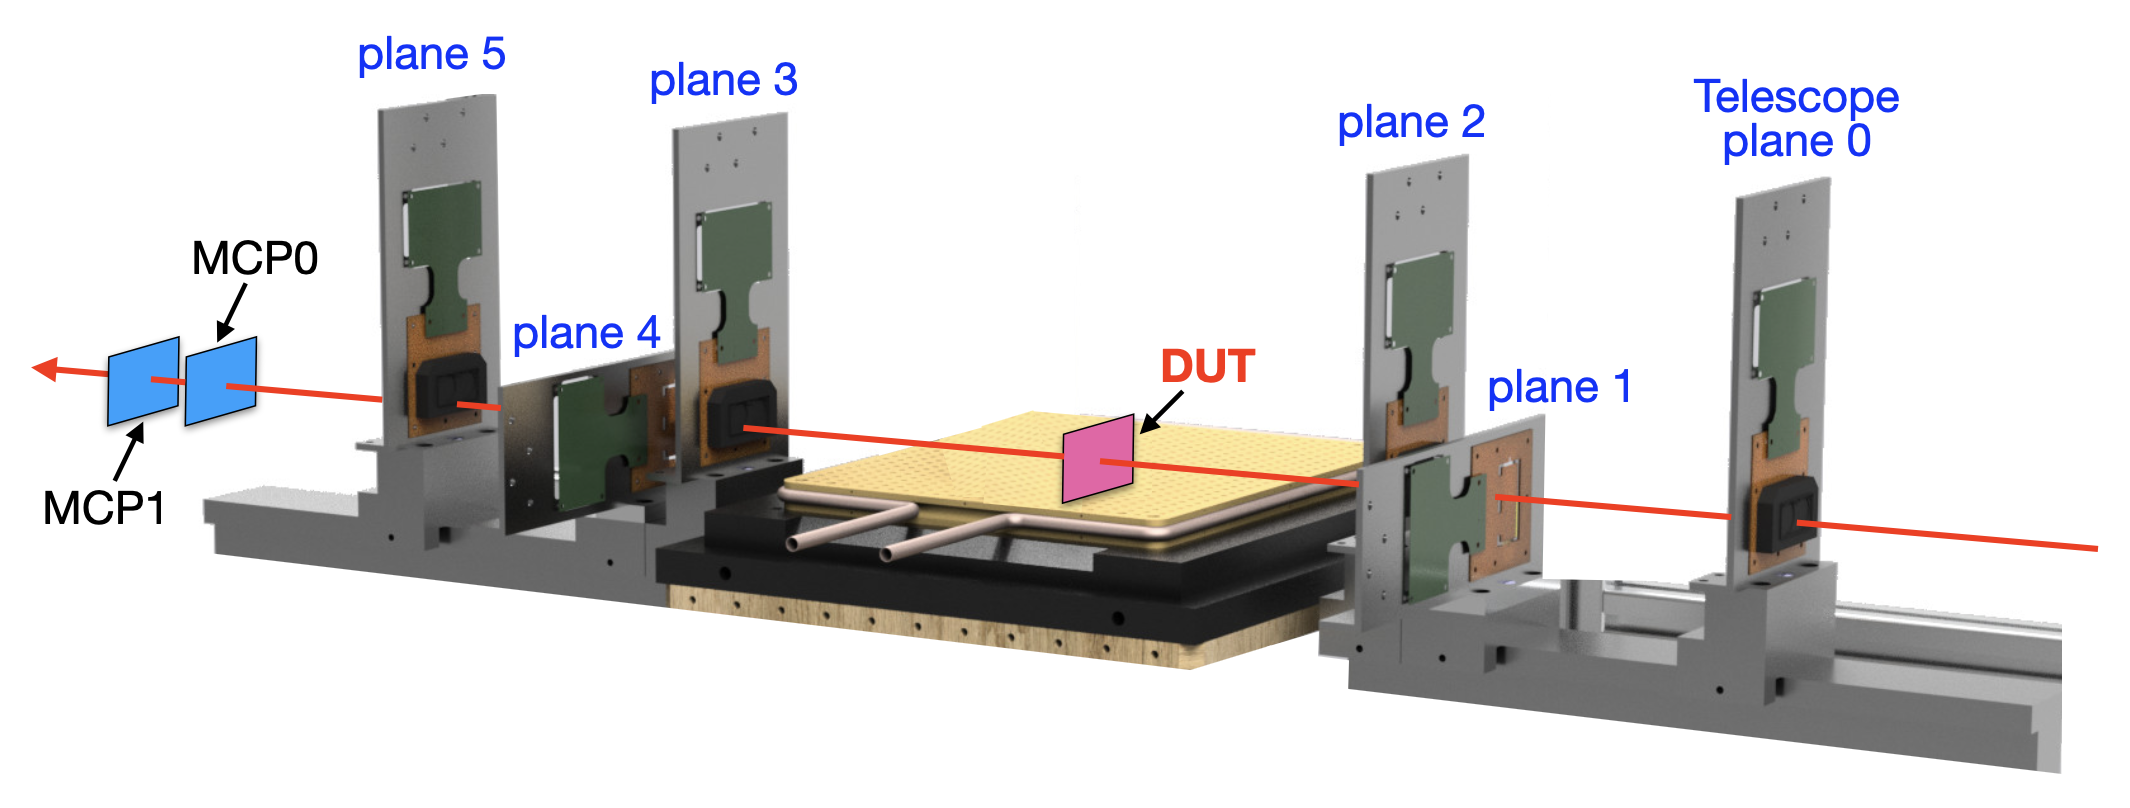
\includegraphics[width=0.9\linewidth]{files/MONOLITH_paper/telescope.png}
			\caption{Schematic view of the experimental setup, showing the six planes of the UniGe FE-I4 telescope \cite{telescope}, the DUT, and the two MCPs installed downstream the telescope with respect to the pion beam direction.}
			\label{im:MONO_Setup} x
		\end{figure}

		Analog signals from all detectors were read by two oscilloscopes. A first oscilloscope with a sampling rate of 40 GS/s and an analog bandwidth set to 4 GHz was used to read the two MCP detectors and the differential output from pixel OA0 of the DUT. Pixels OA1, OA2 and OA3 of the DUT were instead connected to a second oscilloscope with 4 GHz analog bandwidth and a sampling rate of 20 GS/s. The oscilloscopes produced a saturation of the signal amplitudes to around \SI{75}{\milli\volt} for all the DUT pixels. 

		The FE-I4 telescope provided the trigger signal to the oscilloscopes, with a region of interest of $250 \times 250 $ $\mu$ m$^2$ imposed to the first telescope plane and centred at the pixel OA0. A window of 200 ns around the telescope trigger time was defined to record waveform data from the oscilloscopes.  


		\subsubsection{Telescope-Track Selection Criteria}
		Pion trajectories and their point of intersection with the DUT were reconstructed using the hits recorded by the FE-I4 telescope planes. To maximise the telescope pointing resolution, tracks were required to have hits in all six telescope planes and $ \chi^{2}/NDF \le 1.5 $. To suppress ambiguous cases, events with more than one reconstructed track were rejected. For tracks satisfying the aforementioned criteria, the telescope pointing resolution on the DUT plane was estimated in \cite{vicente_thesis} to be approximately \SI{10}{\um} in both directions.
		
		\begin{figure}[!htb]
			\centering
			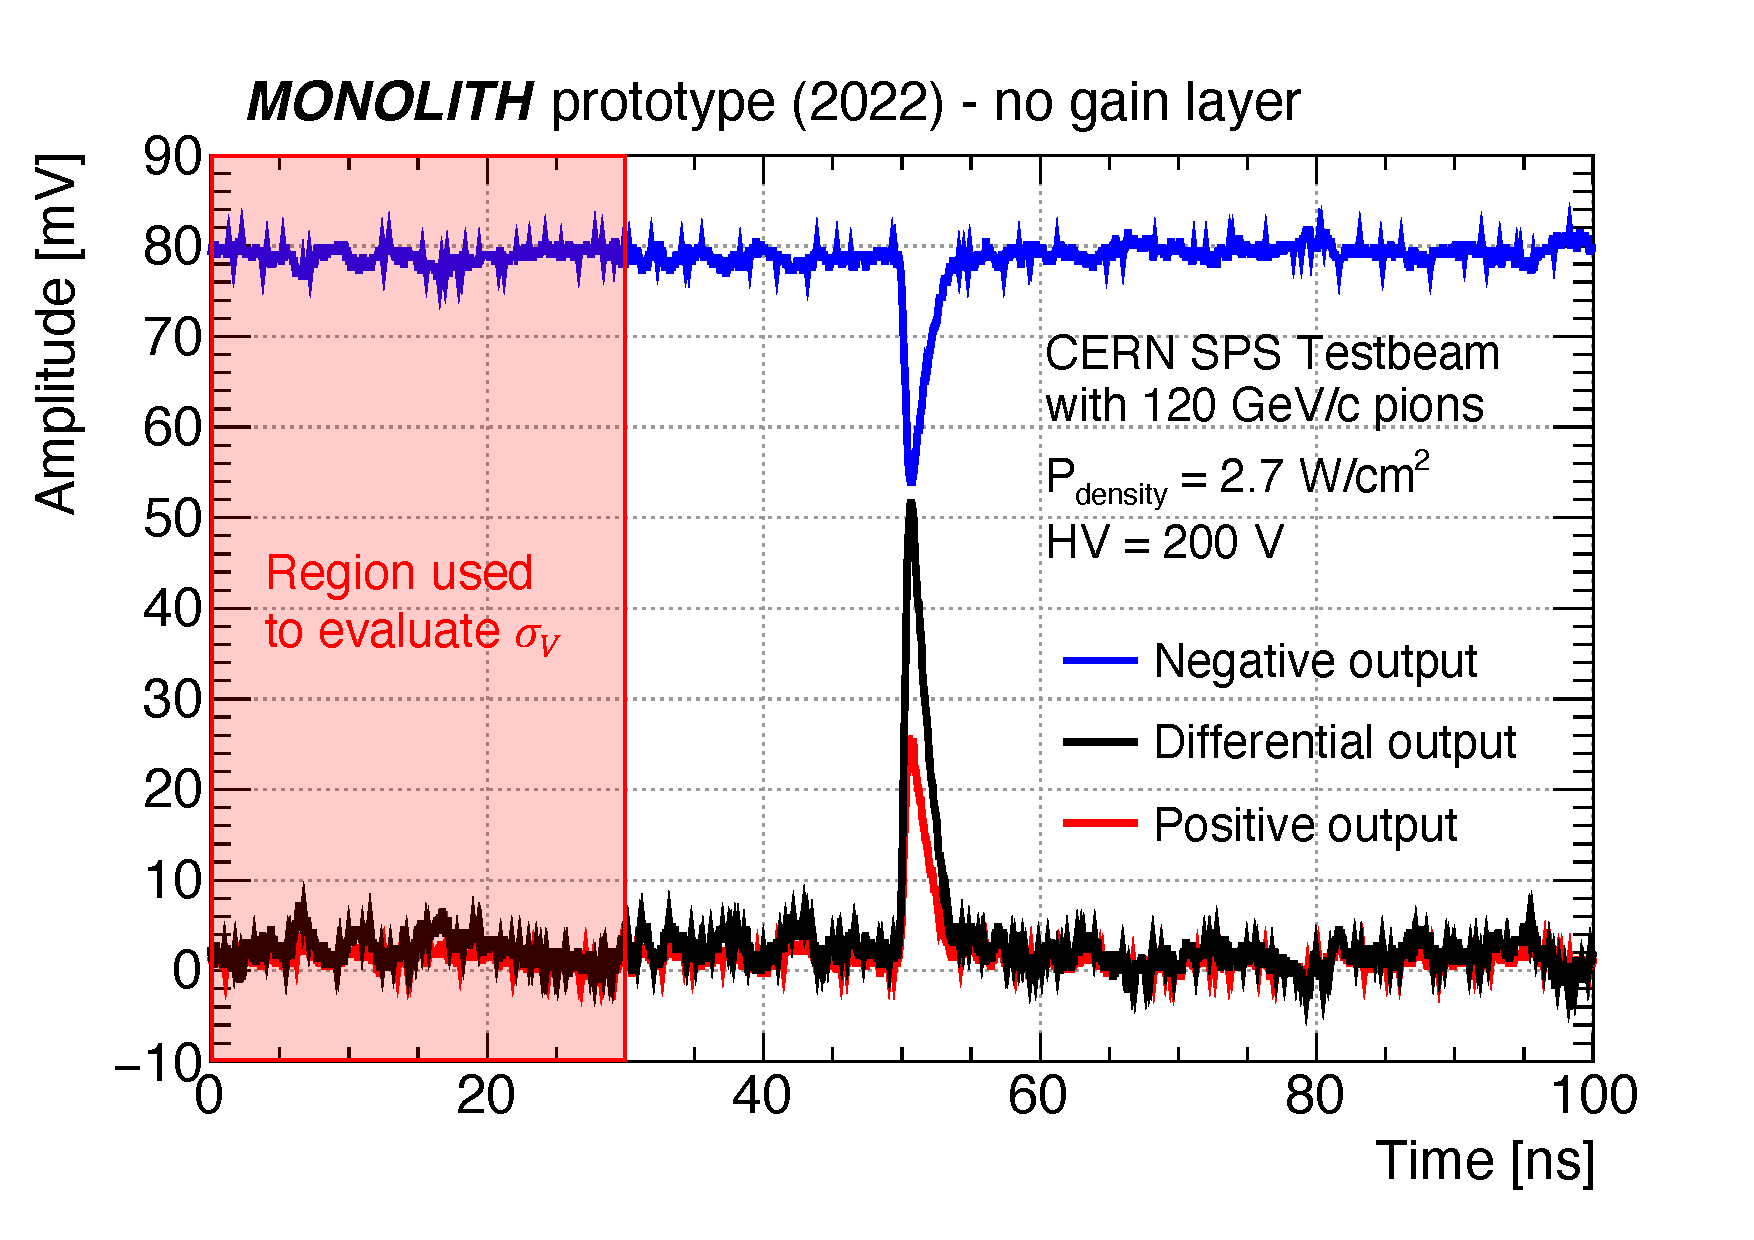
\includegraphics[width=.49\textwidth]{files/MONOLITH_paper/waveform_with_bck_region.pdf}
			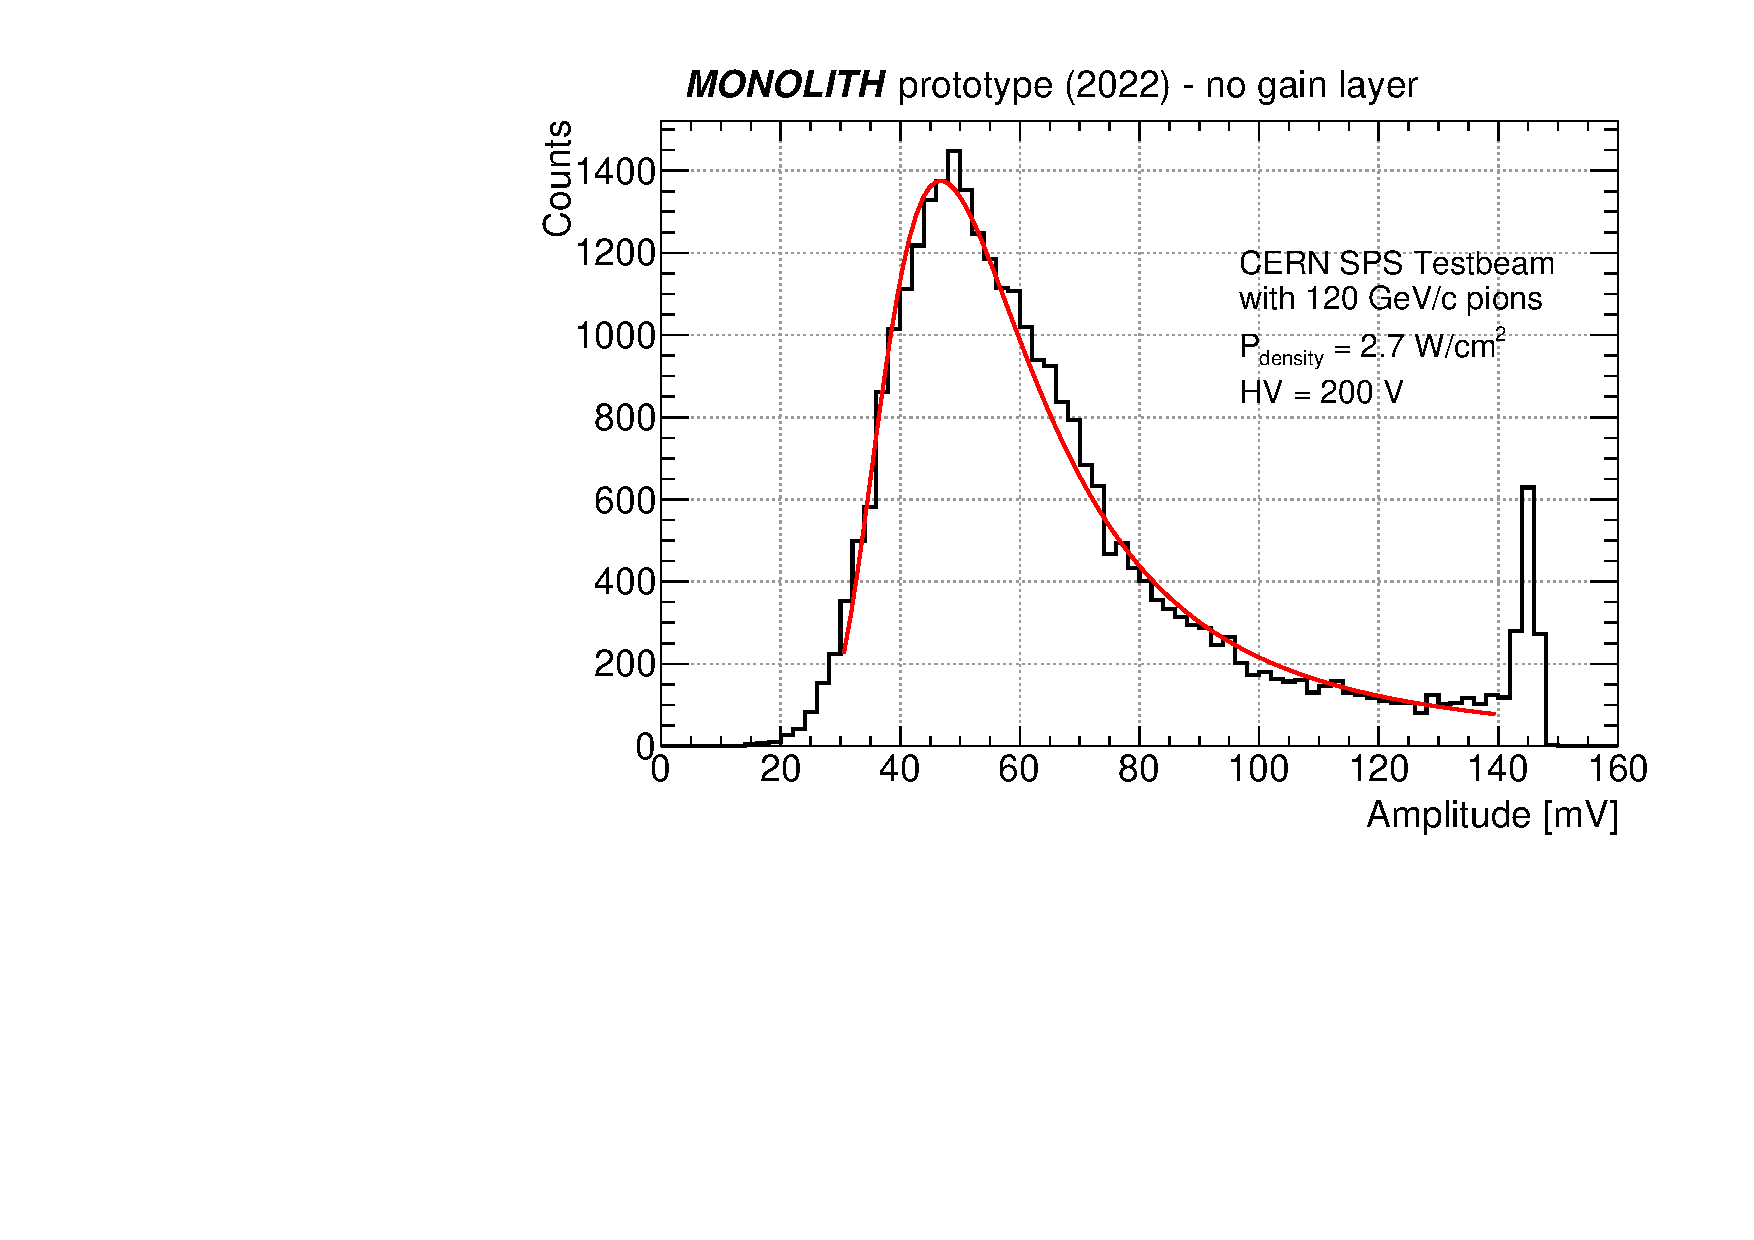
\includegraphics[width=.49\textwidth]{files/MONOLITH_paper/amplitude.pdf}
			\caption{Characteristics of signals from  pixel OA0 with the DUT operated at power density \power = \SI{2.7}{\watt/\centi\meter^2} and bias voltage $HV=$\SI{200}{\volt}. Example of waveforms from the single-ended outputs with the two polarities (blue and red) and from the differential one (black). The analog signal amplitudes from pixel OA0 were sampled every $\SI{25}{\pico\second}$.  The voltage noise \noise was extracted taking the standard deviation of the differential signal amplitudes in the time interval between 0 and 30 ns (left). Distribution of the amplitudes of the differential signals; the peak at large values is generated by the saturation of the oscilloscope. The red line is the result of a fit using a Landau functional form (right).}
			\label{im:MONO_waveform} 
		\end{figure}

		\subsubsection{Data samples}
		Large samples of data were acquired at the four sensor bias voltage values $HV$ = 120, 160, 200 and 250 V, and at the five power density values reported in Table \ref{tab:MONO_gain}.
		For all these working points, the samplings of the differential signal in the first 30 ns of the trigger time window were used to determine the standard deviation of the voltage noise $\sigma_V$ of the DUT at the output of the analog front end. The left panel of Figure \ref{im:MONO_waveform} shows a typical waveform acquired for pixel OA0 of the DUT operated at power density \power \SI{2.7}{\watt/\centi\meter^2} and bias voltage $HV=$ \SI{200}{\volt}.
		The distribution of the differential signal amplitudes from pixel OA0 after the telescope-track selection is shown in the right panel of Figure \ref{im:MONO_waveform}.

		\subsection{Detection Efficiency}
		The pion tracks reconstructed by the FE-I4 telescope and surviving the analysis selection criteria were used to measure the DUT detection efficiency. The efficiency was computed as the ratio between the number of selected tracks associated to recorded signals with amplitudes above a threshold of 7 times the voltage noise \noise and the total number of selected tracks traversing the DUT in the area corresponding to the four analog pixels. A tolerance of \SI{10}{\micro\meter} in the region outside the external boundaries of the four-pixel area was allowed to account for the finite telescope pointing resolution.

		\begin{figure}[h]
			\centering
			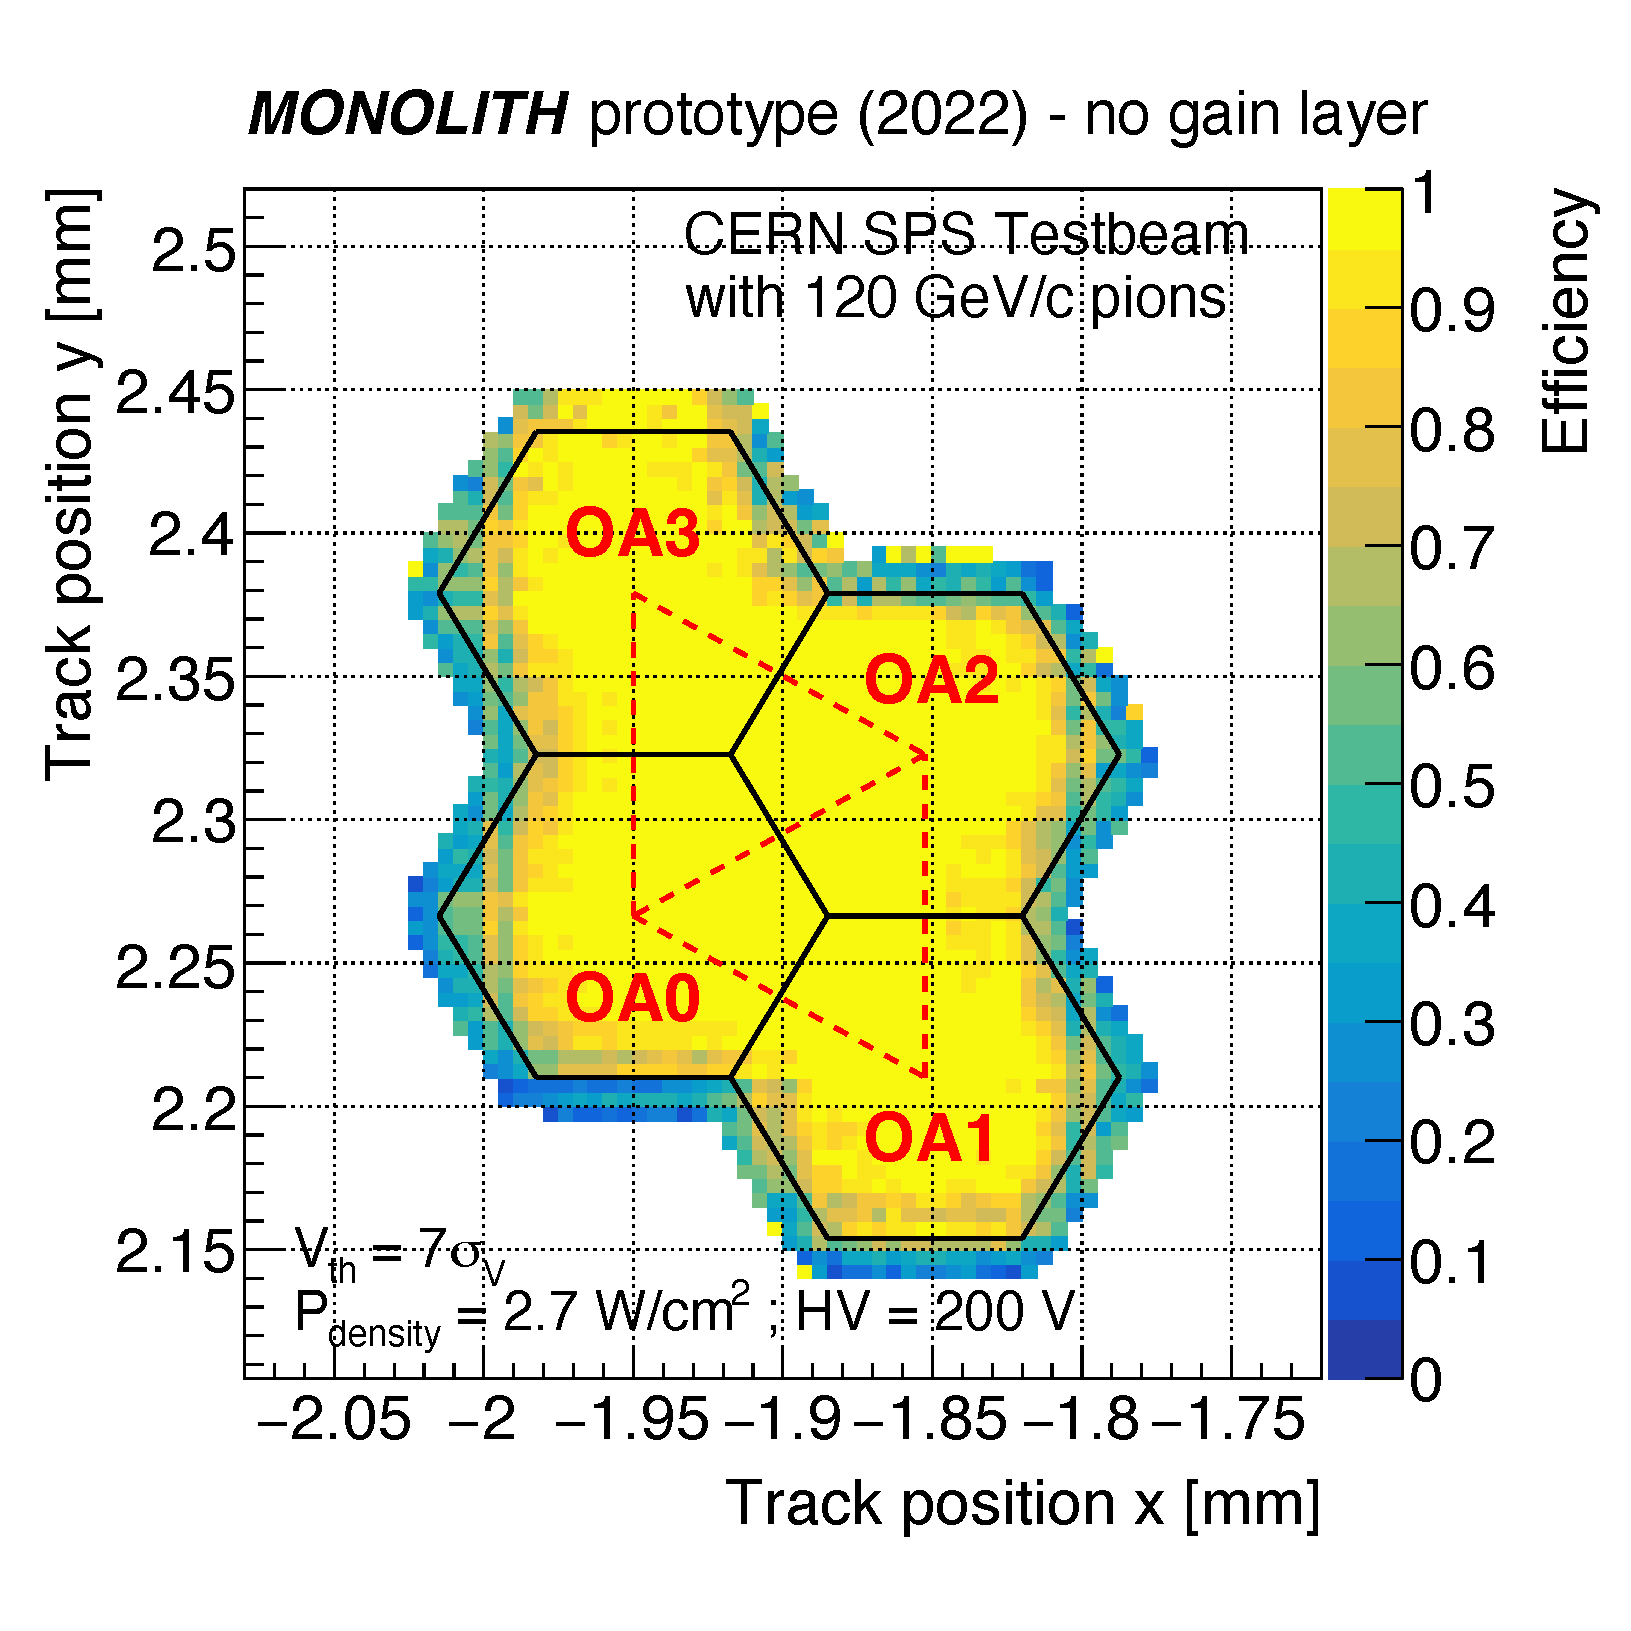
\includegraphics[width=.49\textwidth,trim=0 0 0 0]{files/MONOLITH_paper/WP1_HV200V_efficiency_map.pdf}
			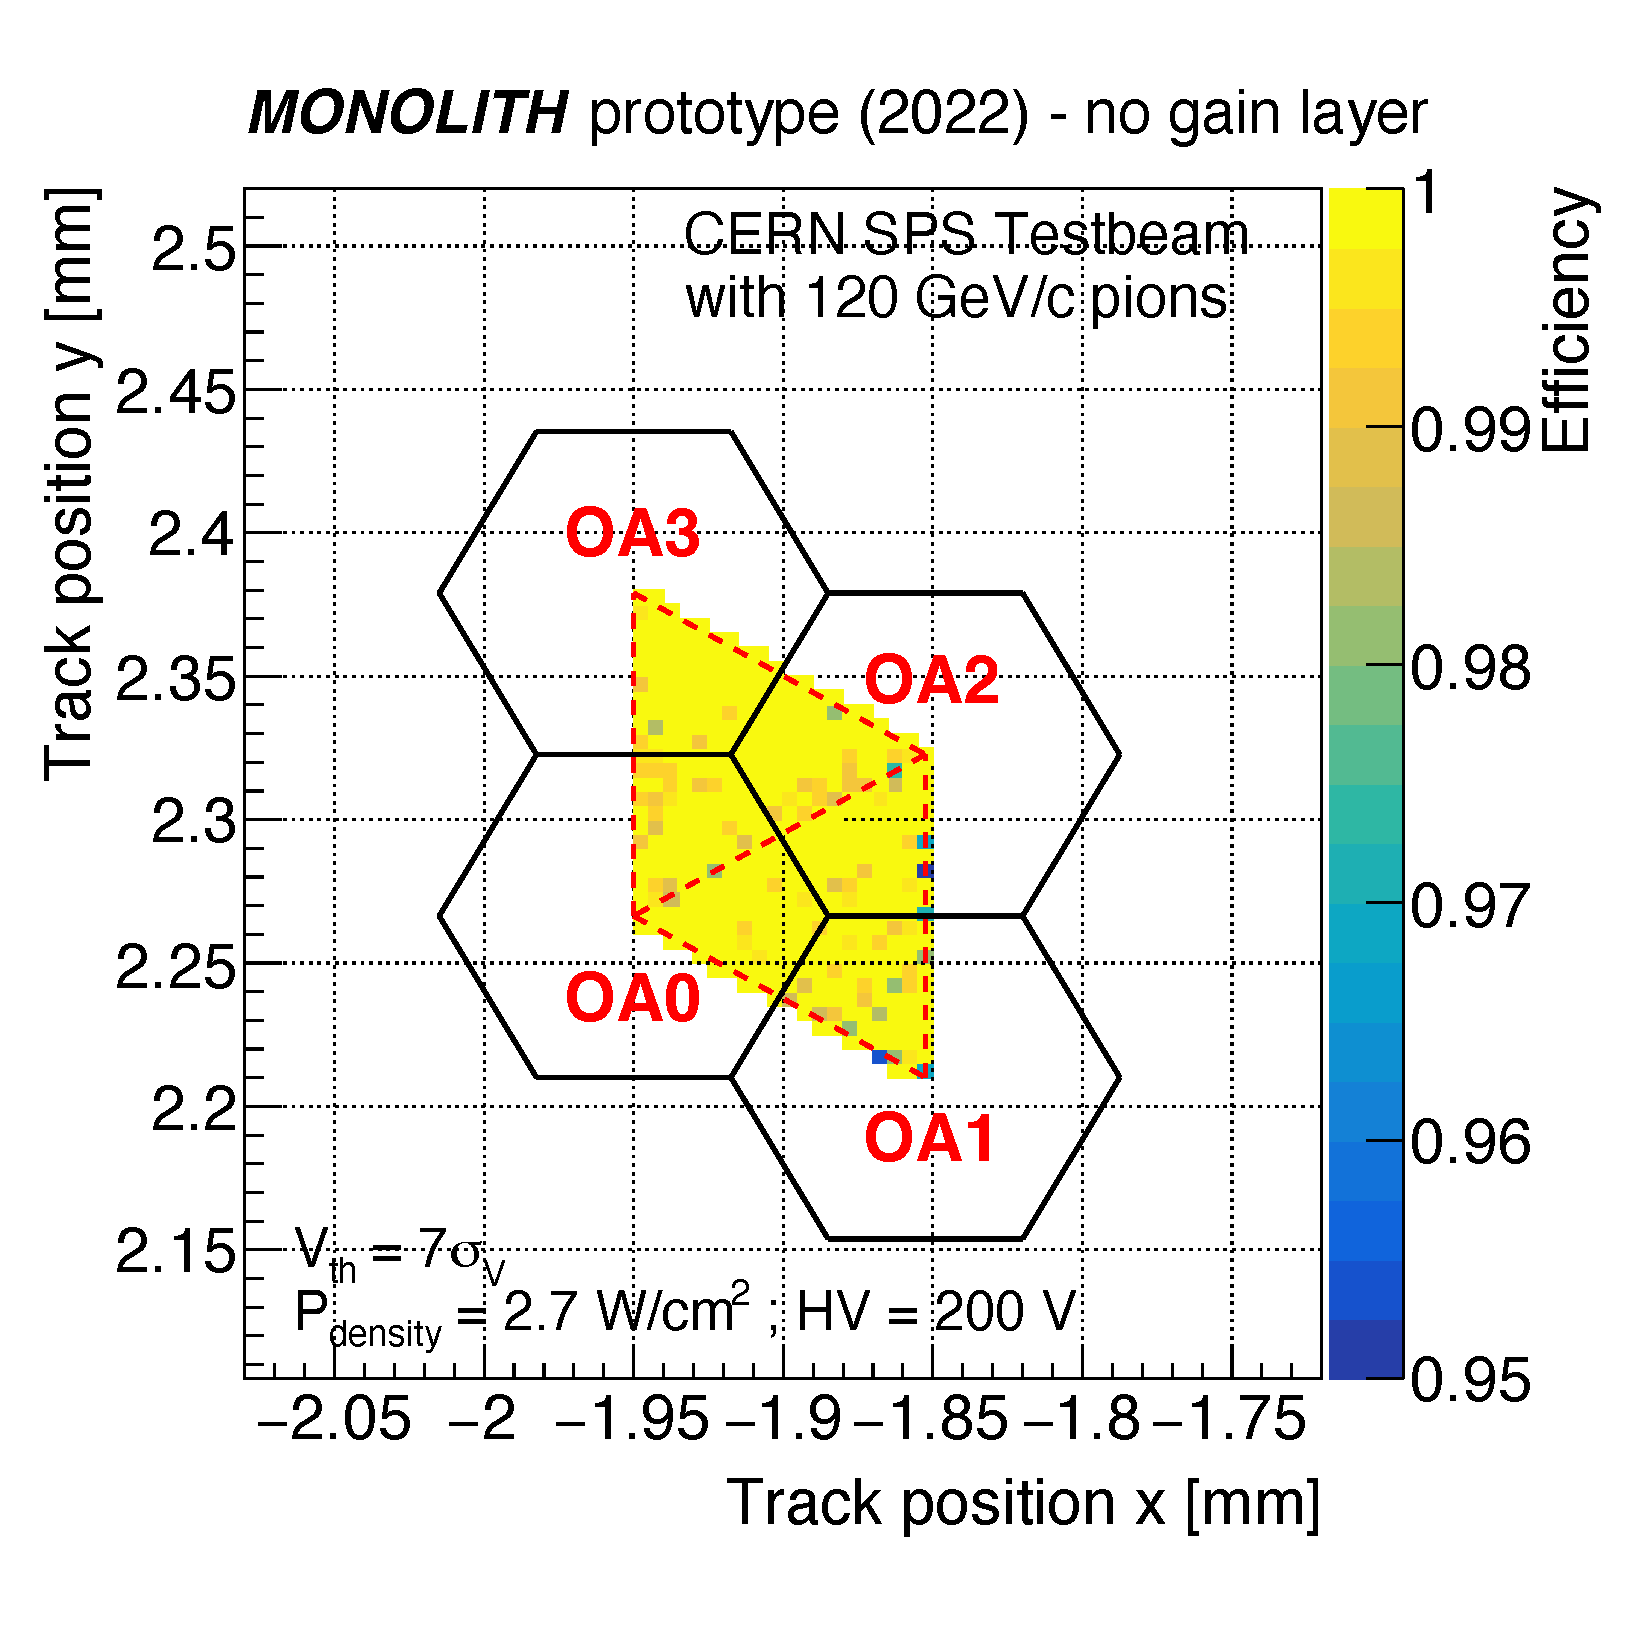
\includegraphics[width=.49\textwidth,trim=0 0 0 0]{files/MONOLITH_paper/WP1_HV200V_triangles_map.pdf}
			\caption{Detection efficiency measured for the \textit{MONOLITH} prototype operated at power density \power = \SI{2.7}{\watt/\centi\meter^2} and $HV=$ \SI{200}{\volt}, with a discrimination threshold of 7\noise. (Left) Measurement performed in a region that extends beyond the pixel edges (black lines) by \SI{10}{\micro\meter}. The apparent decrease of the efficiency at the external boundaries delimiting the area of the four instrumented pixels is produced by the finite FE-I4 telescope pointing resolution. (Right) Efficiency measured in the two triangular areas which is unaffected by the resolution of the telescope; the colour scale of the plot starts at 95\% efficiency.}
			\label{im:MONO_effmap} 
		\end{figure}

		Figure \ref{im:MONO_effmap} shows the results of the efficiency measurement for the DUT operated at \power = \SI{2.7}{\watt/\centi\meter^2} and $HV=$ \SI{200}{\volt}. As shown by the left panel, the finite FE-I4 telescope pointing resolution generates an apparent inefficiency close to the 14 external edges of the four pixels (and an efficiency outside them), which makes the evaluation of the efficiency in the total pixel area difficult. Since this effect is not present in the five internal edges of the four pixels, the measurement was repeated selecting only tracks extrapolated inside the two triangles connecting the OA0--OA2--OA3 and OA0--OA2--OA1 pixel centres. 
		The result is shown in the right panel of Figure \ref{im:MONO_effmap}, in which the colour scale starts at 95\%. It should be noted that the two triangles contain all the relevant pixel regions, such as the boundary between two pixels and the corner between three pixels, in the same proportion as in an entire pixel. For all the working points, the efficiencies measured separately in the two triangles were found to be compatible within statistics, and thus averaged. The efficiency value measured inside the two triangles for the working point of Figure \ref{im:MONO_effmap} is ($ 99.86_{-0.04}^{~\!+0.03} $)\%, as reported in the second row of Table \ref{tab:MONO_eff_ipream_HV_pscan}.

		\begin{table}[h]
			\centering 
			\renewcommand{\arraystretch}{1.4}
			%%%%%%%%%%%%%%%%%%%%%%%%%%%%%%%%%%%%%%%%%%
			\begin{tabular}{|c|c|c|}
			\cline{1-3}
			 \power [W/cm$^2$] & ~~~~~~~$HV$~[\si{V}]~~~~~~~  & Average efficiency [\%] \\
			\cline{1-3}
			2.7   & 250 & $ 99.80_{-0.09}^{~\!+0.07} $ \\
			2.7   & 200 & $ 99.86_{-0.04}^{~\!+0.03} $ \\
			2.7   & 160 & $ 99.71_{-0.10}^{~\!+0.08} $ \\
			2.7   & 120 & $ 99.80_{-0.09}^{~\!+0.07} $ \\
			0.9   & 200 & $ 99.83_{-0.04}^{~\!+0.04} $ \\
			0.36  & 200 & $ 99.81_{-0.05}^{~\!+0.04} $ \\
			0.13  & 200 & $ 99.77_{-0.05}^{~\!+0.04} $ \\
			0.04  & 200 & $ 99.86_{-0.07}^{~\!+0.05} $ \\
			\cline{1-3}
			\end{tabular}
			\caption{Detection efficiency measured for the \textit{MONOLITH} prototype at different power density and sensor bias voltage values. A voltage threshold of 7 \noise is applied. The efficiencies are measured separately in the two triangular areas shown in Figure \ref{im:MONO_effmap}, and then averaged.}
			\label{tab:MONO_eff_ipream_HV_pscan}
		\end{table} 

		It is interesting to characterise the dependence of the detection efficiency on the discrimination threshold, as it is influenced by the signal to background ratio of the sensor. The result for the DUT operated at \power = \SI{2.7}{\watt/\centi\meter^2} and $HV=$ \SI{200}{\volt} is shown in Figure \ref{im:MONO_effthrscan}.
		\begin{figure}[h]
			\centering 
			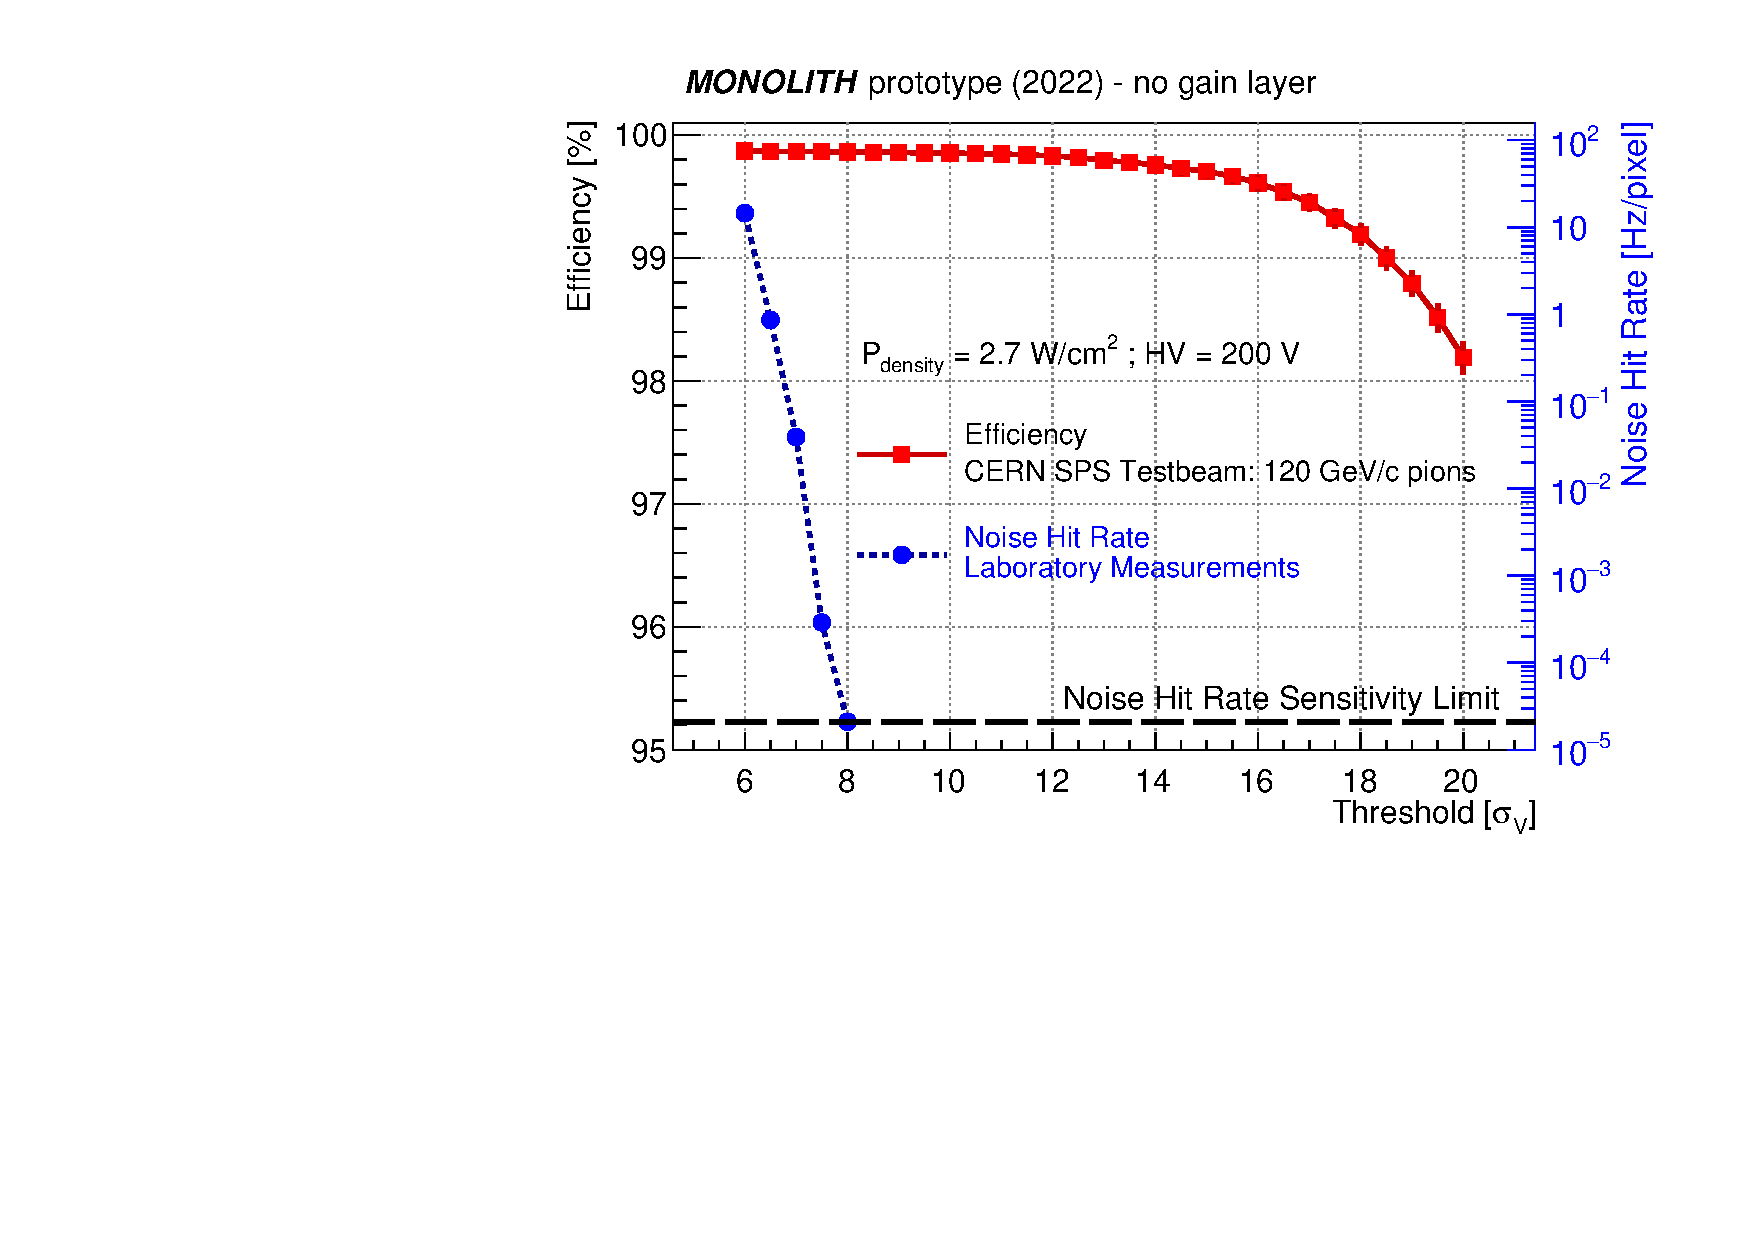
\includegraphics[width=0.67\linewidth]{files/MONOLITH_paper/eff_fhr_vs_thr.pdf}
			\caption{Detection efficiency (red squares) and noise-hit rate (blue circles) measured within the two triangular areas depicted in Figure \ref{im:MONO_effmap}, as a function of the voltage threshold in integer multiples of the the voltage noise \noise. The data refer to sensor bias $ HV =$ \SI{200}{\volt} and power density \power = \SI{2.7}{\watt/\centi\meter^2}.}
			\label{im:MONO_effthrscan} 
		\end{figure}
	
		 Remarkably, the efficiency remains above 99 $\%$ up to threshold values of 18 times the voltage noise. 
		A voltage threshold of 7 \noise was used throughout the data analysis, which corresponds to approximately 600 electrons for this working point. Figure \ref{im:MONO_effthrscan} reports also the noise-hit rate measured in the laboratory, which is $2.9\cdot 10^{-4}$ Hz/pixel at 7\noise, corresponding approximately to 1 noise hit every hour. In the testbeam data sample taken at this working point, we expect less than 1 noise hit.
		

		Table~\ref{tab:eff_ipream_HV_pscan} and Figure~\ref{fig:eff_ipream_HV_pscan} show the average efficiency in the two triangles for the eight working points at which data were acquired. 
		%Similarly, the average efficiencies are shown in Figure~\ref{fig:eff_ipream_HV_pscan} as a function of the power density $P_{\mathrm {\it density}}$ and the sensor bias voltage $HV$. 
		Within the statistical uncertainty, no significant trend is observed: all the efficiencies are found to be compatible with 99.8\%. Figure~\ref{fig:eff_radius} shows  the DUT efficiencies measured as a function of the distance from the pixel center for the eight working points acquired. In all cases the efficiencies remain remarkably stable around 99.8\% within the whole pixel area, showing that no drop in the inter-pixel region is measured.

		\begin{figure}[h]
			\centering 
			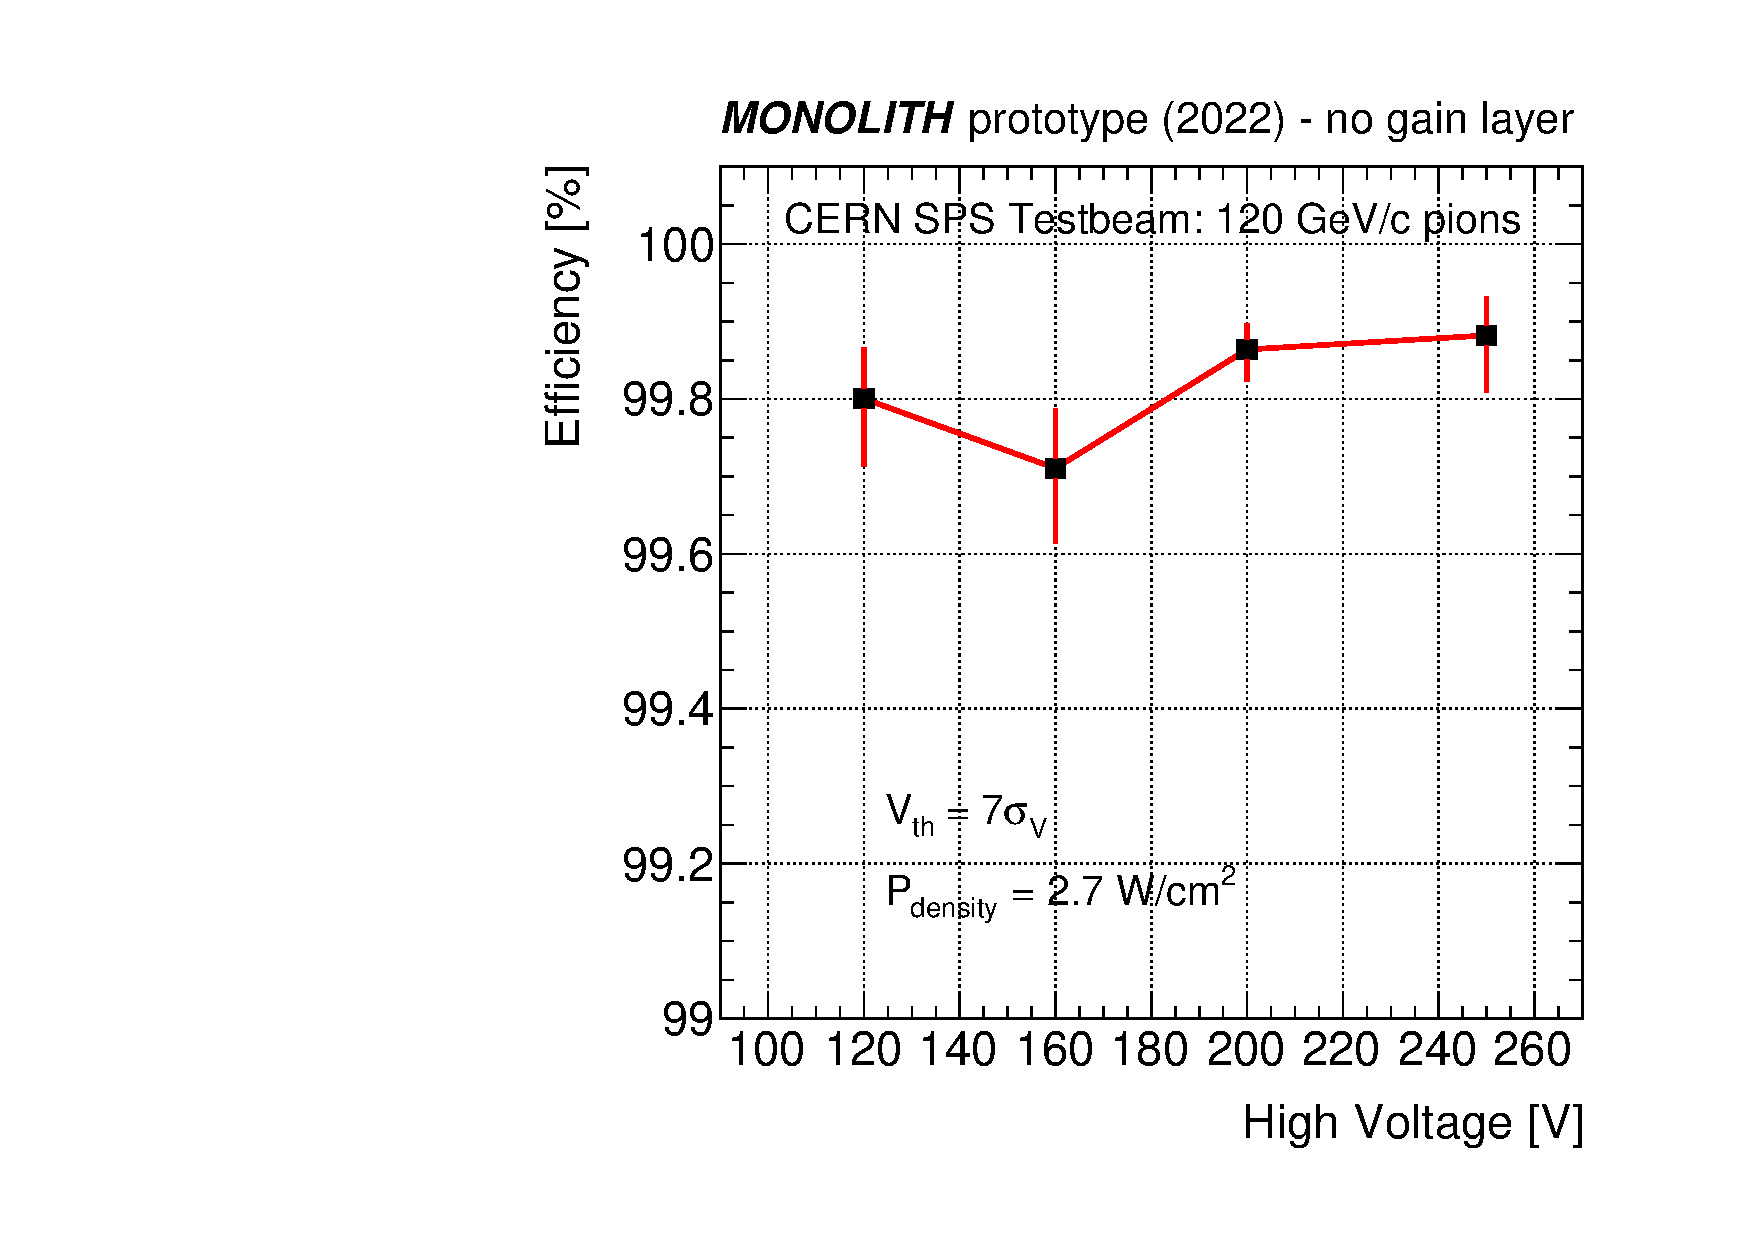
\includegraphics[width=.49\textwidth,trim=0 0 0 0]{files/MONOLITH_paper/eff_HV.pdf}
			\includegraphics[width=.49\textwidth,trim=0 0 0 0]{files/MONOLITH_paper/eff_power.pdf}
			\caption{Detection efficiency measured within the two triangular areas depicted in Figure \ref{im:MONO_effmap} with $V_{\mathrm {\it th}}=7~\!\sigma_V$. In the left panel, the efficiency is measured at four values of sensor bias voltage for a power density of 2.7 W/cm$^2$. In the right panel, the measurement is shown for five power density values at sensor bias $HV=\SI{200}{\volt}$.}
			\label{im:MONO_eff_ipream_HV_pscan}
		\end{figure}

		\begin{figure}[h]
			\centering 
			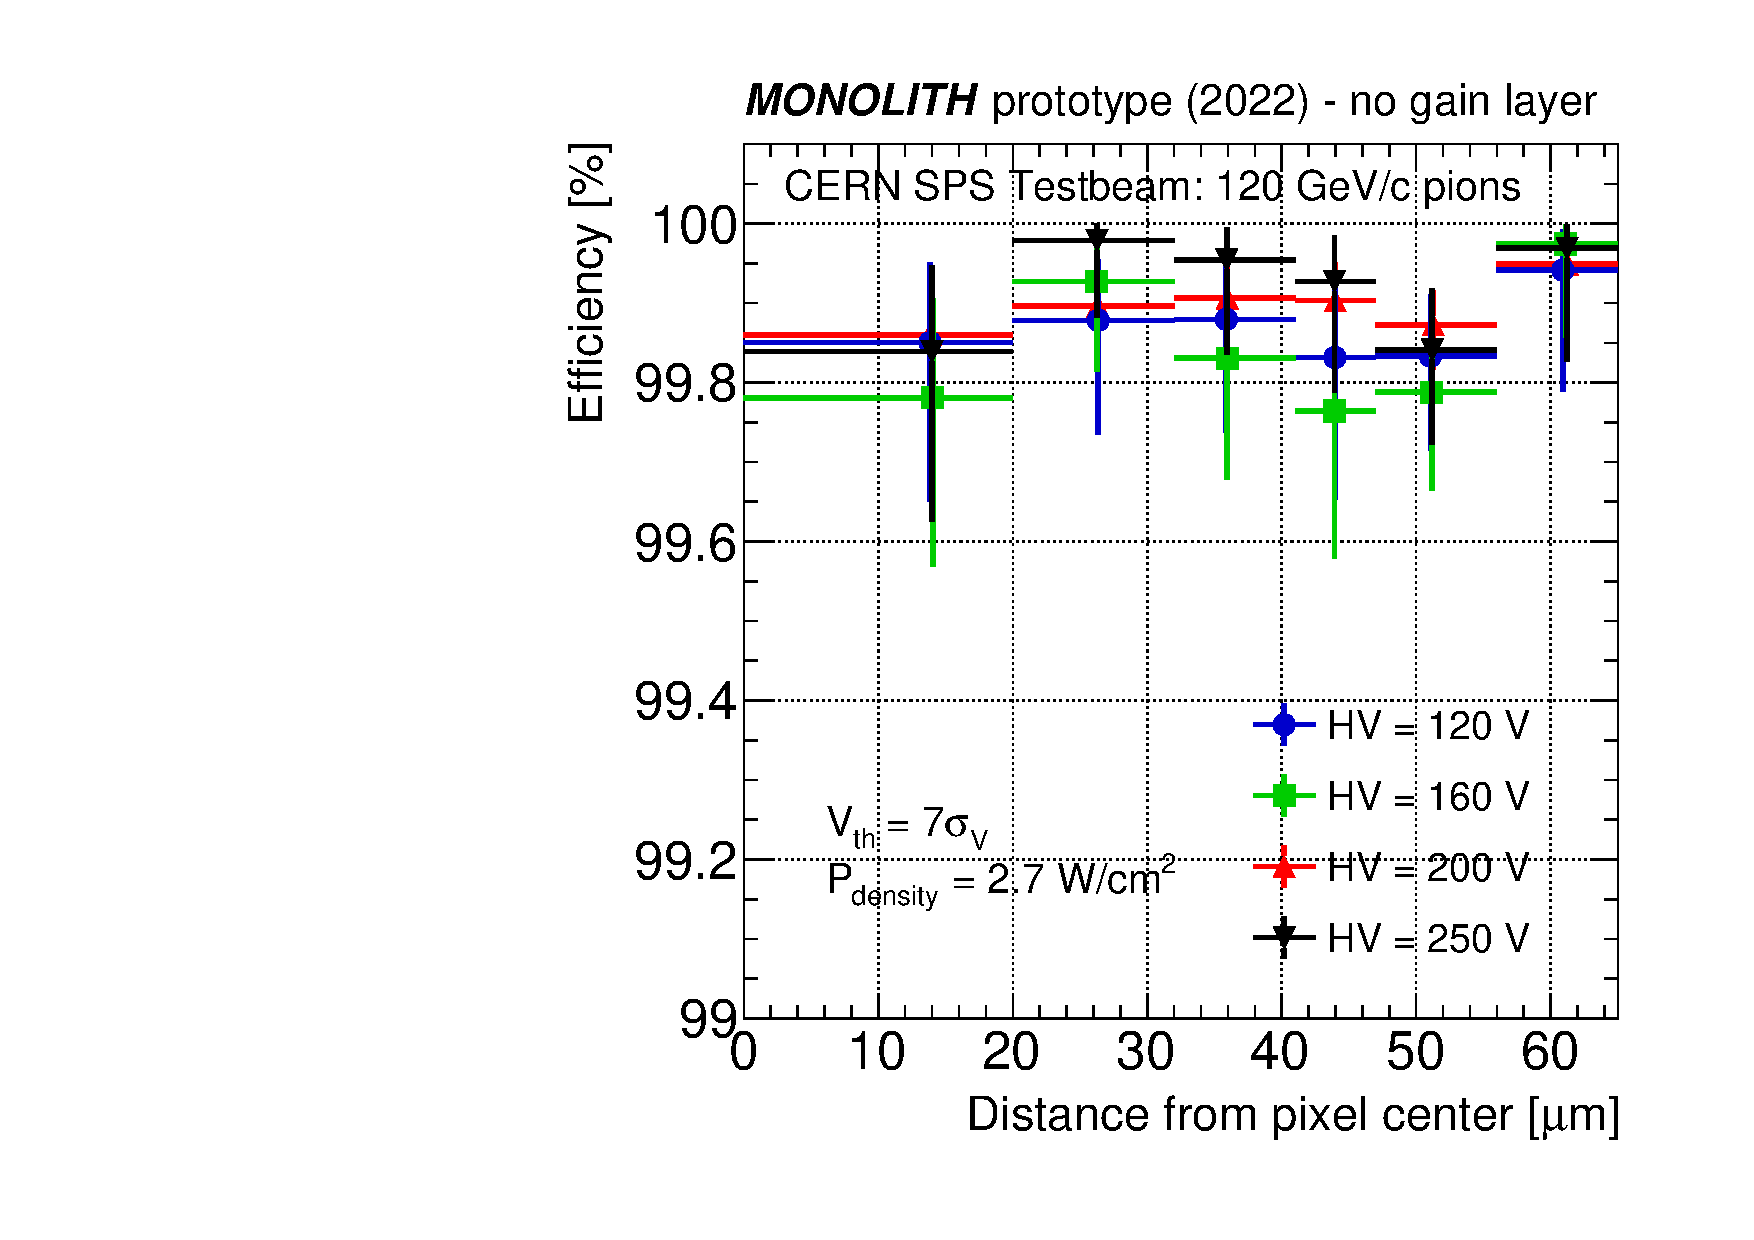
\includegraphics[width=.49\textwidth,trim=0 0 0 0]{files/MONOLITH_paper/eff_vs_radius_HV.pdf}
			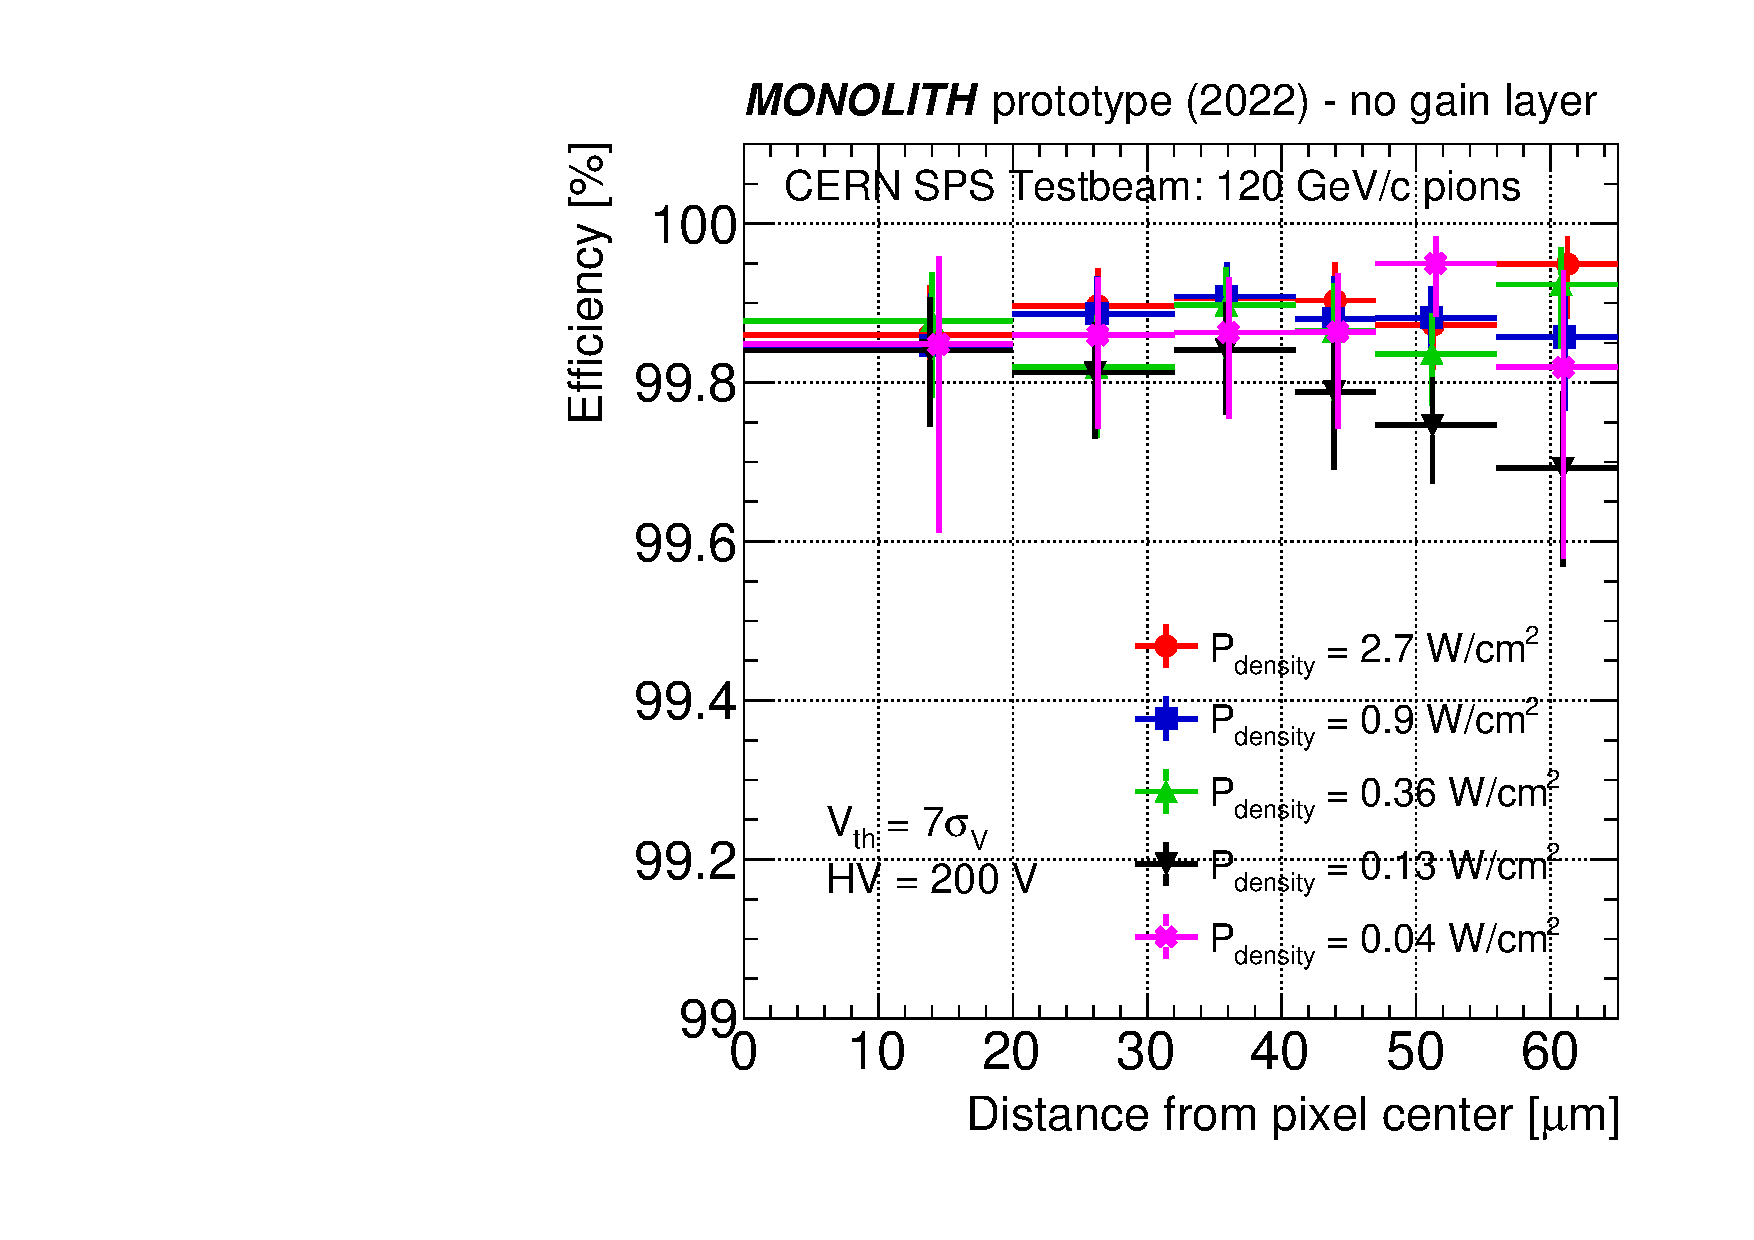
\includegraphics[width=.49\textwidth,trim=0 0 0 0]{files/MONOLITH_paper/eff_vs_radius_power.pdf}
			\caption{Detection efficiency measured within the two triangular areas depicted in Figure \ref{im:MONO_effmap}, in six distance intervals from the corresponding pixel center. In the left panel, the  efficiency is shown for four values of $HV$ at a power density of 2.7 W/cm$^2$. In the right panel, it is shown for five power density values at sensor bias $HV=\SI{200}{\volt}$.  In each bin the data-point marker is placed at the average distance value from the pixel center.}
			\label{im:MONO_eff_radius} 
		\end{figure}













		\subsection{Time Resolution}	

		The time measurements of the DUT and the two MCPs for the sample of tracks selected as described in Section \note{section ref} were used to determine the timing performance of the \textit{MONOLITH} prototype. 
		The DUT time resolution was studied using the time of arrival (\toa) of the  analog signals acquired by pixel OA0, which was connected to the fastest oscilloscope. The measurement was restricted to events with telescope tracks crossing the area of pixel OA0 inside the two triangles shown in Figure \ref{im:MONO_effmap}, to exclude hits in the inter-pixel region that have the majority of the charge shared with the three non-instrumented pixels adjacent to OA0, and thus should not be associated to pixel OA0. 
		The \toa values for the DUT were computed as the time at which the linear interpolation between two consecutive oscilloscope samplings of the differential signal reached the 7 \noise threshold. 
		
		The difference in the measured \toa (\dtoa) between the three possible detector pairs, DUT-MCP0, DUT-MCP1 and MCP0-MCP1, corresponds to the TOF between the detectors. Under the assumption of a Gaussian response of the three detectors, the standard deviations extracted from the corresponding \dtoa distributions, \sigdtoa, are interpreted as the sum in quadrature of the time resolution of the two detectors in the pair. By solving a system of three equations, one for each \sigdtoa value, the three unknown time resolutions \sigdut, \sigmcpzero and \sigmcpone can therefore be retrieved.

		\subsubsection{Time-walk correction}
		The distributions of the \dtoa as a function of the amplitudes of the pairs of detectors was used to correct for time walk. As an example, Figure \ref{im:MONO_twcorr} shows the \dtoa distributions for the DUT-MCP0 and DUT-MCP1 pairs as a function of the DUT signal amplitude
		for the working point with power density of \power = \SI{2.7}{\watt/\centi\meter^2} and $HV =$ \SI{200}{\volt}. Two independent methods were deployed and cross-checked against each other to exclude potential biases to the measured timing performance introduced by the time-walk correction procedure. 
		\begin{figure}[!h]
			\centering
			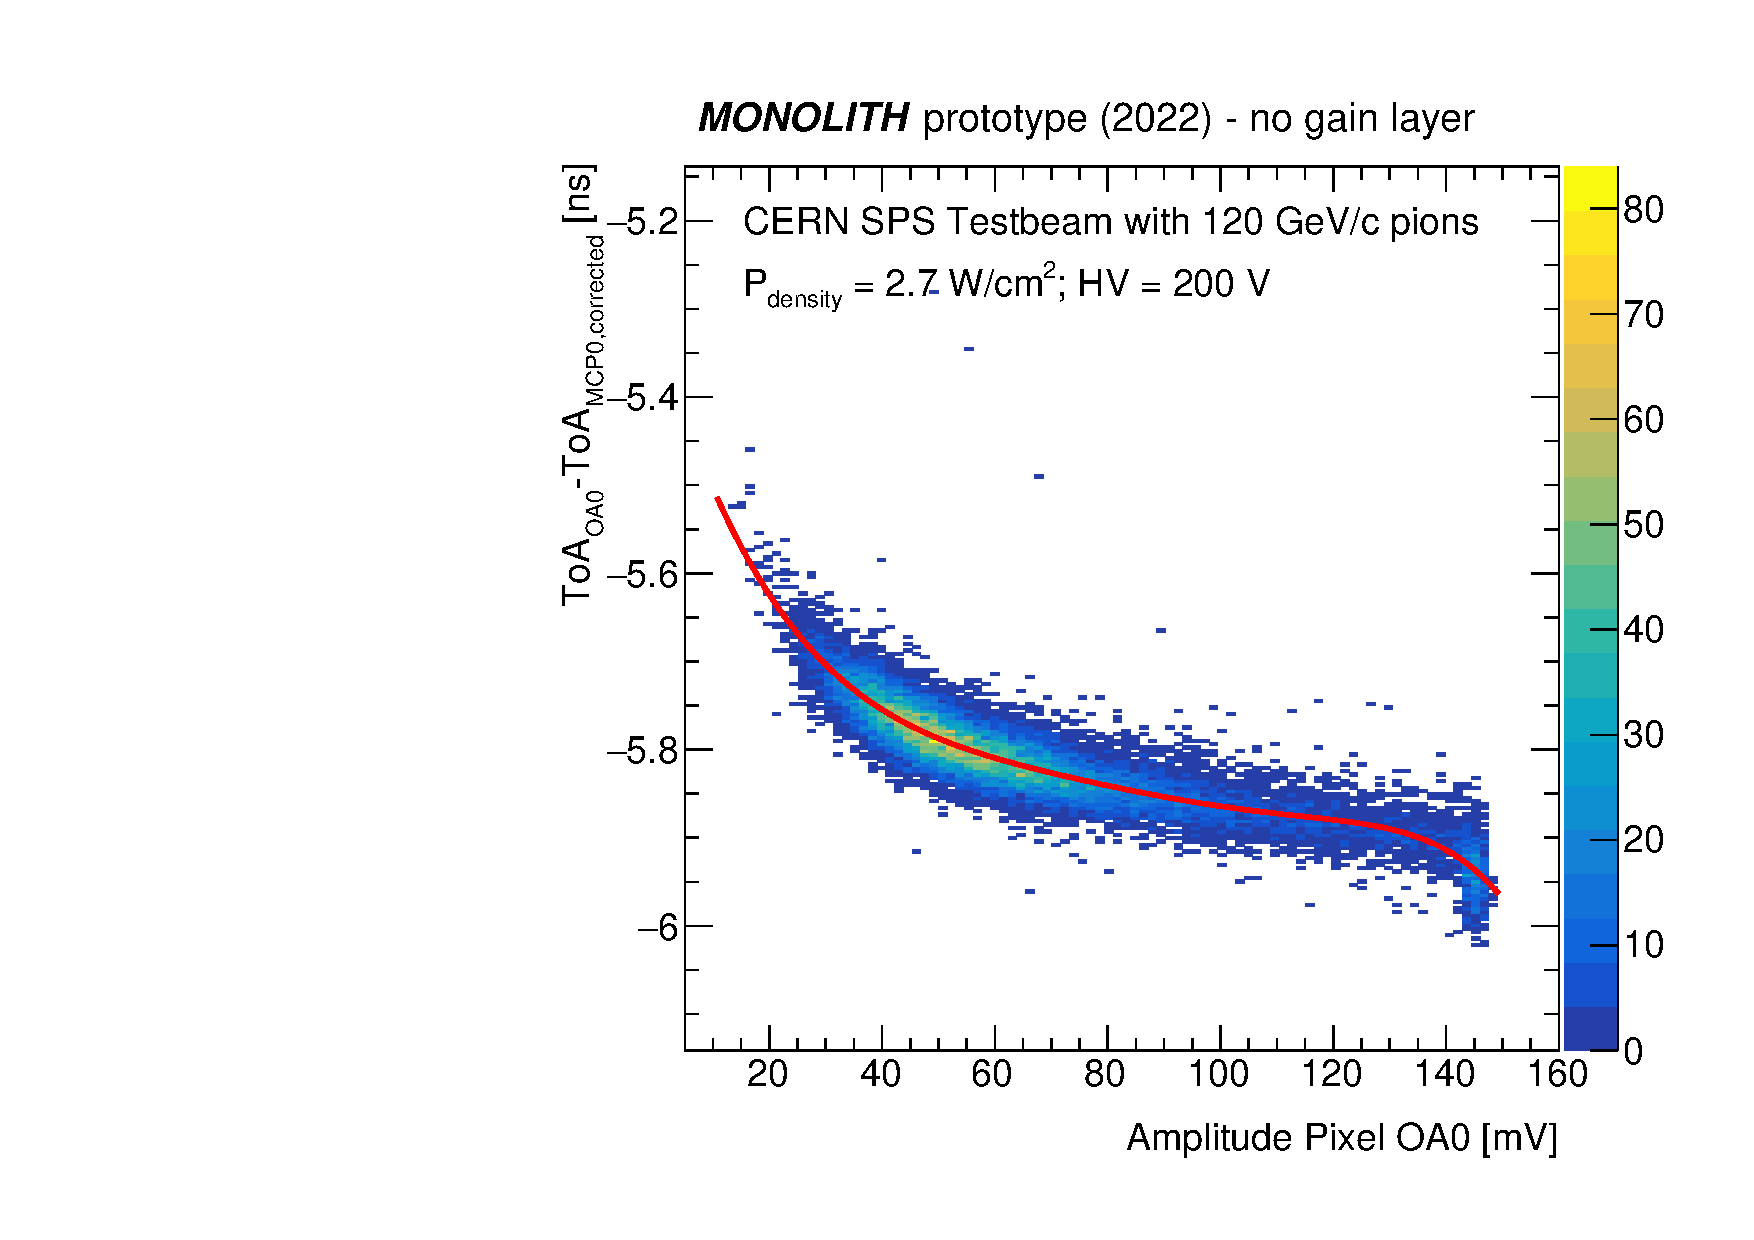
\includegraphics[width=.49\textwidth,trim=0 0 0 0]{files/MONOLITH_paper/TOF_1_vsAmp_1.pdf}
			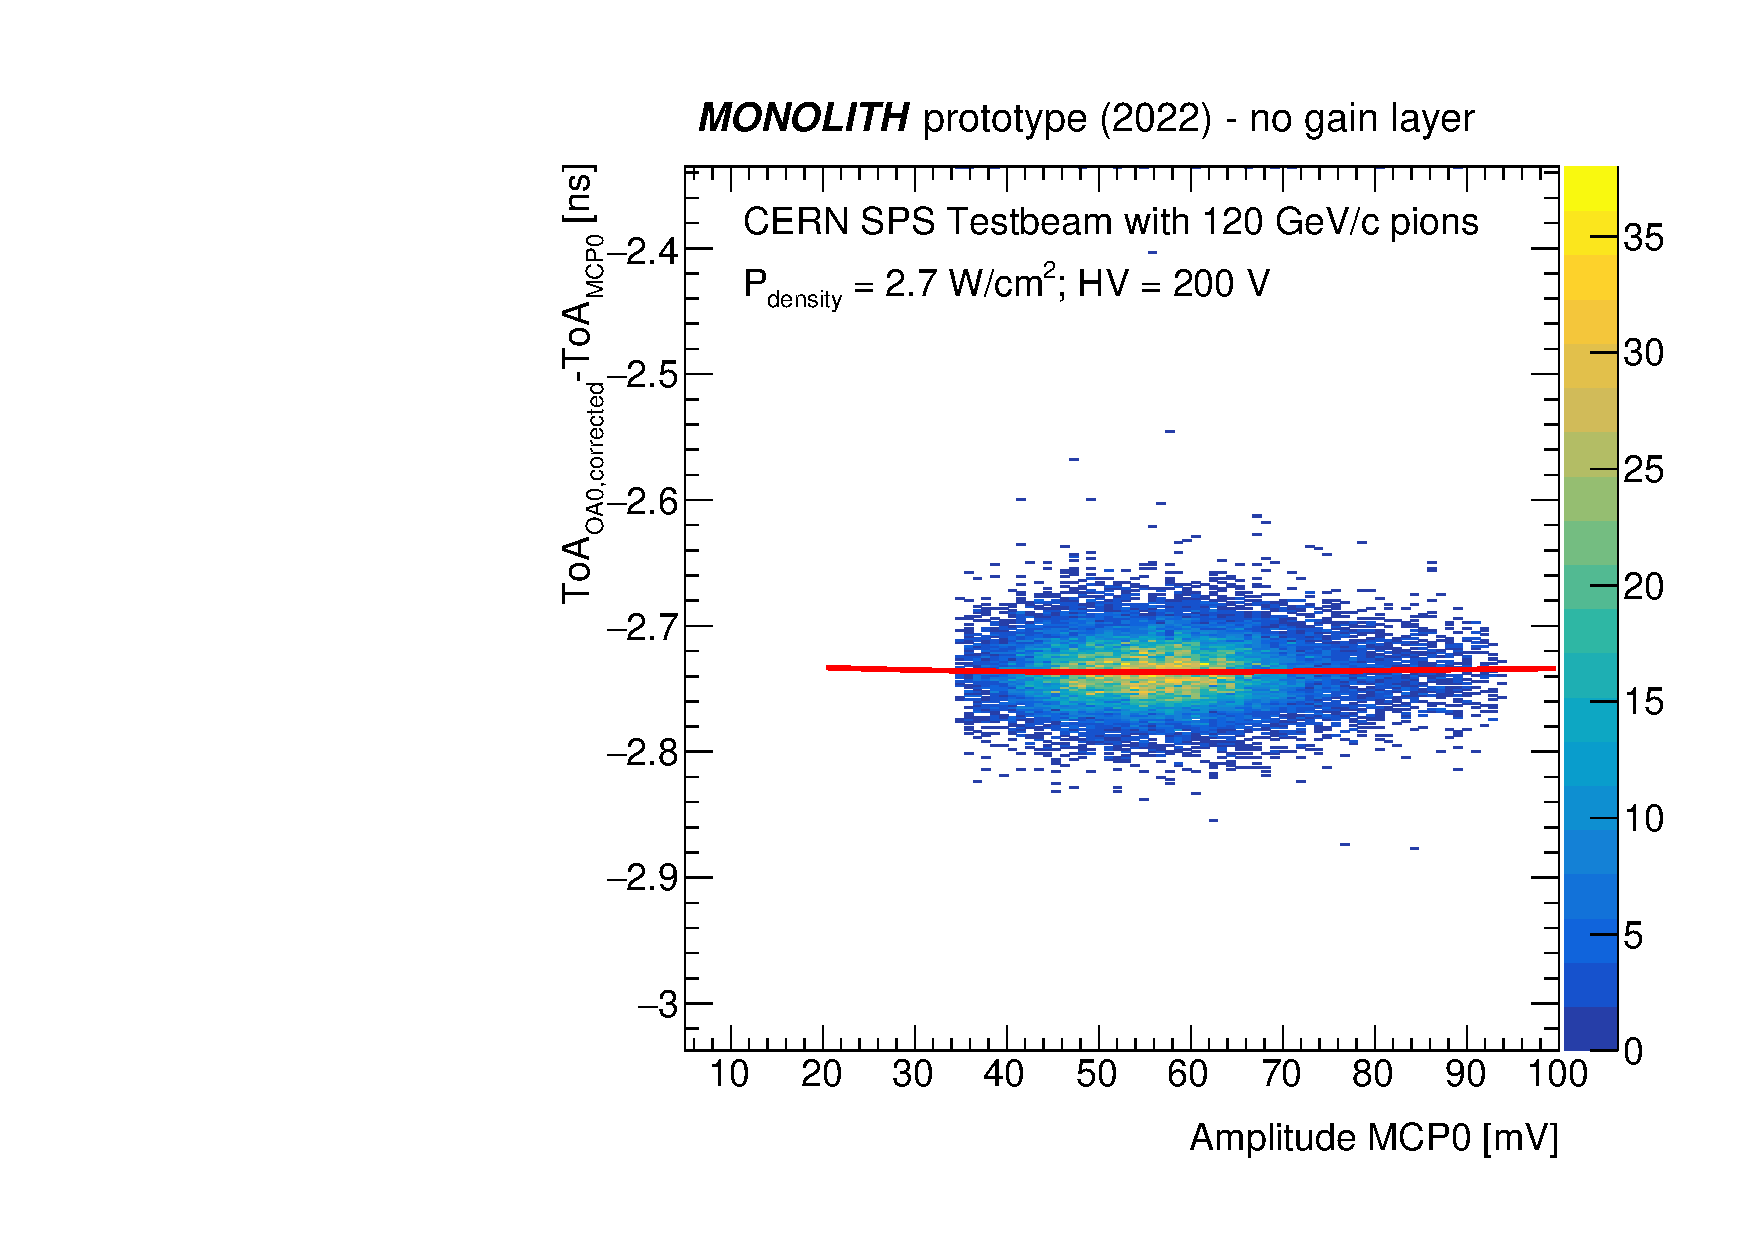
\includegraphics[width=.49\textwidth,trim=0 0 0 0]{files/MONOLITH_paper/TOF_1_vsAmp_2.pdf}
			\caption{\label{fig:twcorr} Distribution of the difference \dtoa between the DUT and MCP0 as a function of the DUT signal amplitude (left), and as a function of the MCP0 signal amplitude (right). The DUT was operated at power density of \power = \SI{2.7}{\watt/\centi\meter^2} and $ HV =$ \SI{200}{\volt}. An arbitrary offset with no influence on the measured time resolution is present in the \toa difference. The red lines show the time-walk corrections obtained with the unbinned maximum likelihood fit method, which were parametrised with polynomial functions with the coefficients determined simultaneously for the three detectors.}
		\end{figure}

		\begin{itemize}
			\item The first correction method is equivalent to the technique used to obtain the results documented in \cite{ATTRACT_proto1_testbeam}. A Gaussian fit to the \dtoa distribution was performed to determine its most probable value, separately for events falling in bins of the signal amplitude. The values obtained were linearly interpolated, resulting in a continuous parametrisation of the correction as a function of the signal amplitude. Each event was then corrected two times, once for each of the detectors involved in the \dtoa. 

			\item The second method relies on an unbinned maximum likelihood fit to extract the time-walk corrections, modelled with polynomial functions $f_\text{DUT}$, $f_\text{MCP0}$ and $f_\text{MCP1}$ of the corresponding signal amplitudes, simultaneously for all detectors. A likelihood estimator $\mathcal{L}$ was constructed under the assumption of a Gaussian time response from all sensors. The probability of observing a \dtoaid difference for a selected track $i$ and the detector pair $d$ can thus be described with a Gaussian probability density function $\mathcal{G}_{i,d}$. In the model, the standard deviation parameter \sigdtoad describes the sum in quadrature of the time resolutions of the two detectors in pair $d$. Additionally, being $d1$ and $d2$ the two detectors involved in the $d$ pair associated to \dtoaid, the total time-walk correction for track $i$ is given by $\mu_{i,d}\equiv f_{d2}(\mathrm{Amplitude}_{d2,i})-f_{d1}(\mathrm{Amplitude}_{d1,i})$. All the parameters of the model were determined by maximising
				\begin{equation}
					\mathcal{L}=\log\left(\prod_i^{\text{tracks}} \prod_d^{\text{detector}\atop\text{pairs}} \mathcal{G}_{i,d}( \Delta_{\text{TOA,i, d}}|\sigma_{\Delta_{\text{TOA,d}}},\mu_{i,d})\right).
				\end{equation}
				A sixth-order polynomial function was chosen for the DUT, in order to model the effect of the amplitude saturation, while third-order polynomials parametrised the time-walk effect for the MCPs. The advantage of this method is the absence of an arbitrary choice of the binning, whilst it is limited by the capability of modeling precisely the functional dependence of the time-walk correction on the signal amplitude.
		\end{itemize}

		These two independent methods yielded results in excellent agreement, with observed differences well below 1 ps, confirming that systematic effects stemming from the extraction of the time-walk correction are marginal.

		\subsubsection{Results}
		For the calculation of the time resolutions, for each working point Gaussian fits of the  time-walk corrected \dtoa distributions of the three pairs of detectors were performed.
		To avoid possible biases of the time-resolution values coming from the non-Gaussian tails, the range of the fit was limited to the bulk of each \dtoa distribution by including only bins populated by more than 25\% of the entries in the bin with the largest content. The $\sigma$ parameters of the Gaussian fits were then used to solve the system of equations that yields the time resolutions for the DUT OA0 and the two MCPs. 

		\begin{figure}[h]
			\centering 
			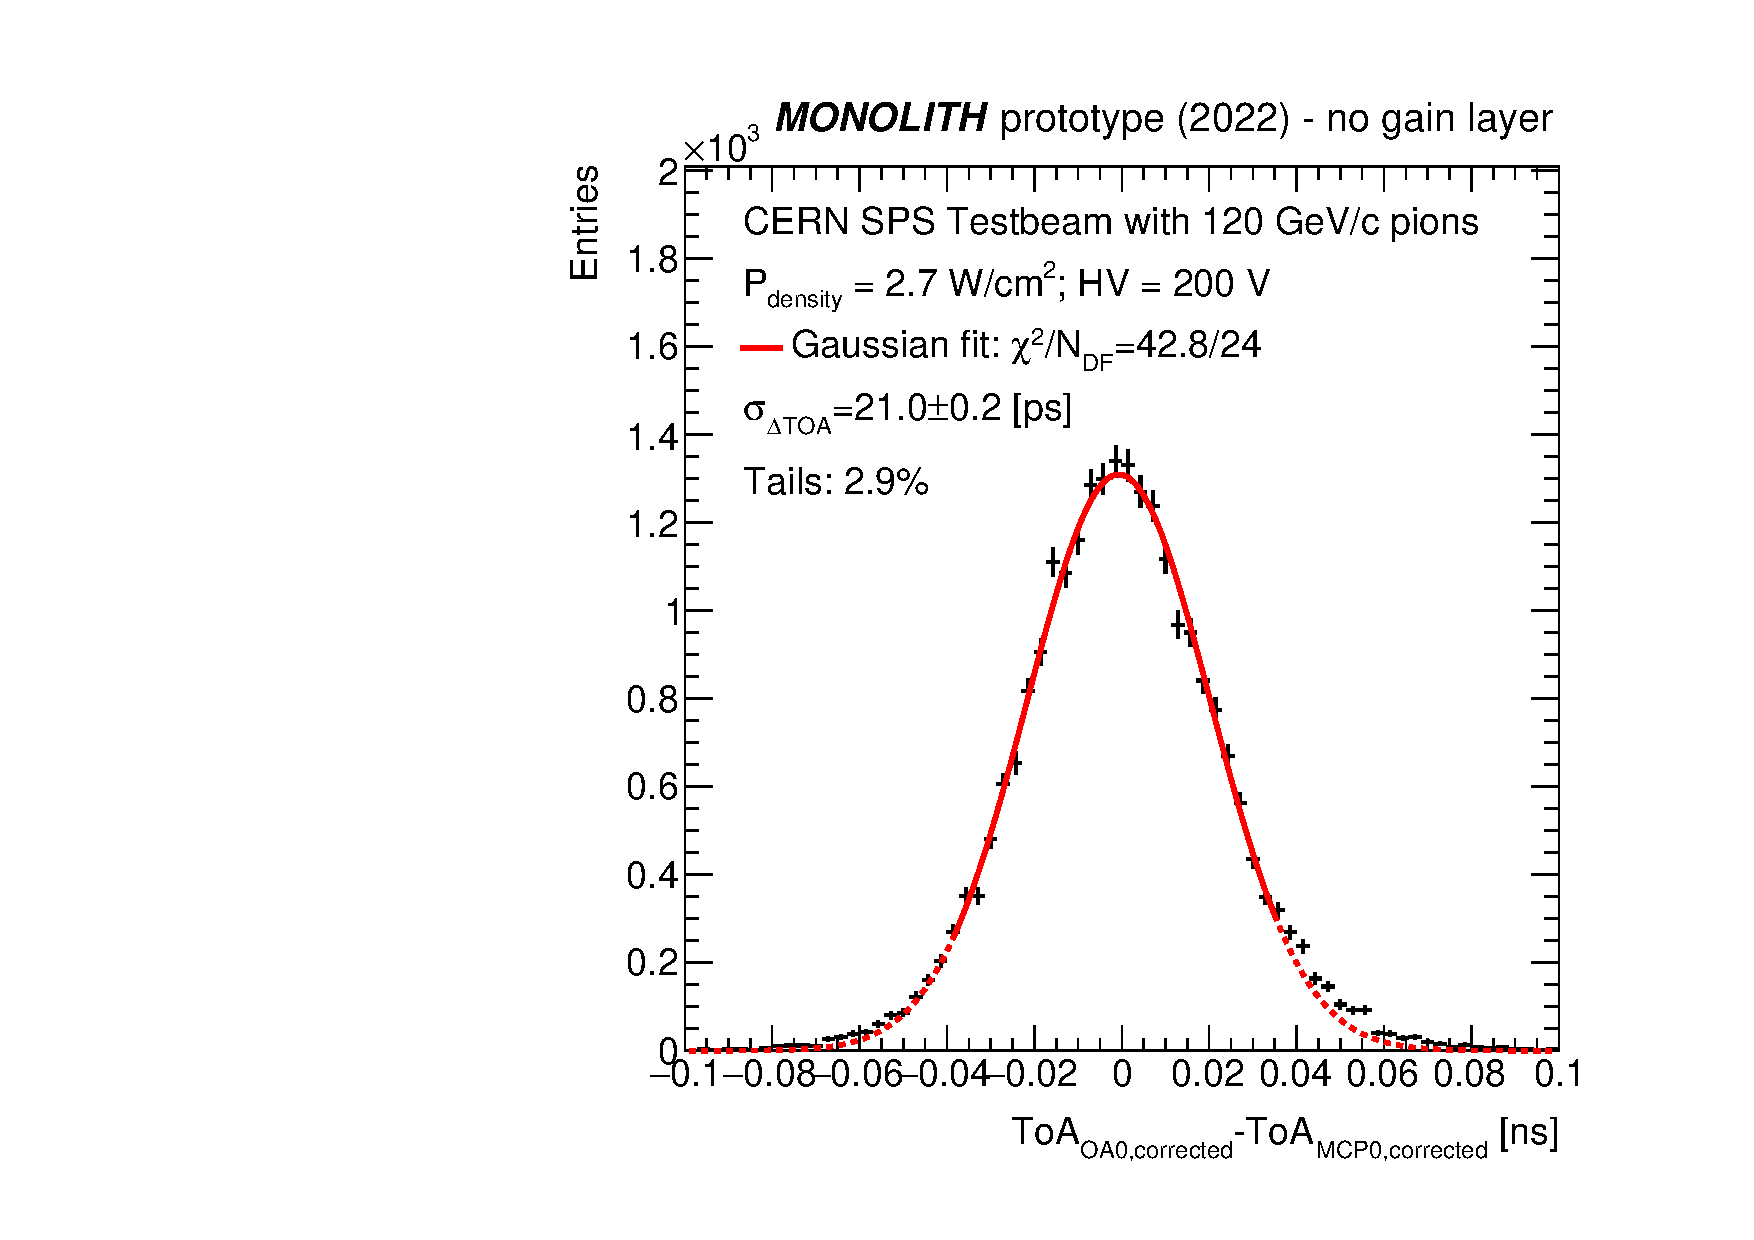
\includegraphics[width=.33\textwidth,trim=40 20 30 20]{files/MONOLITH_paper/TOF_1.pdf}
			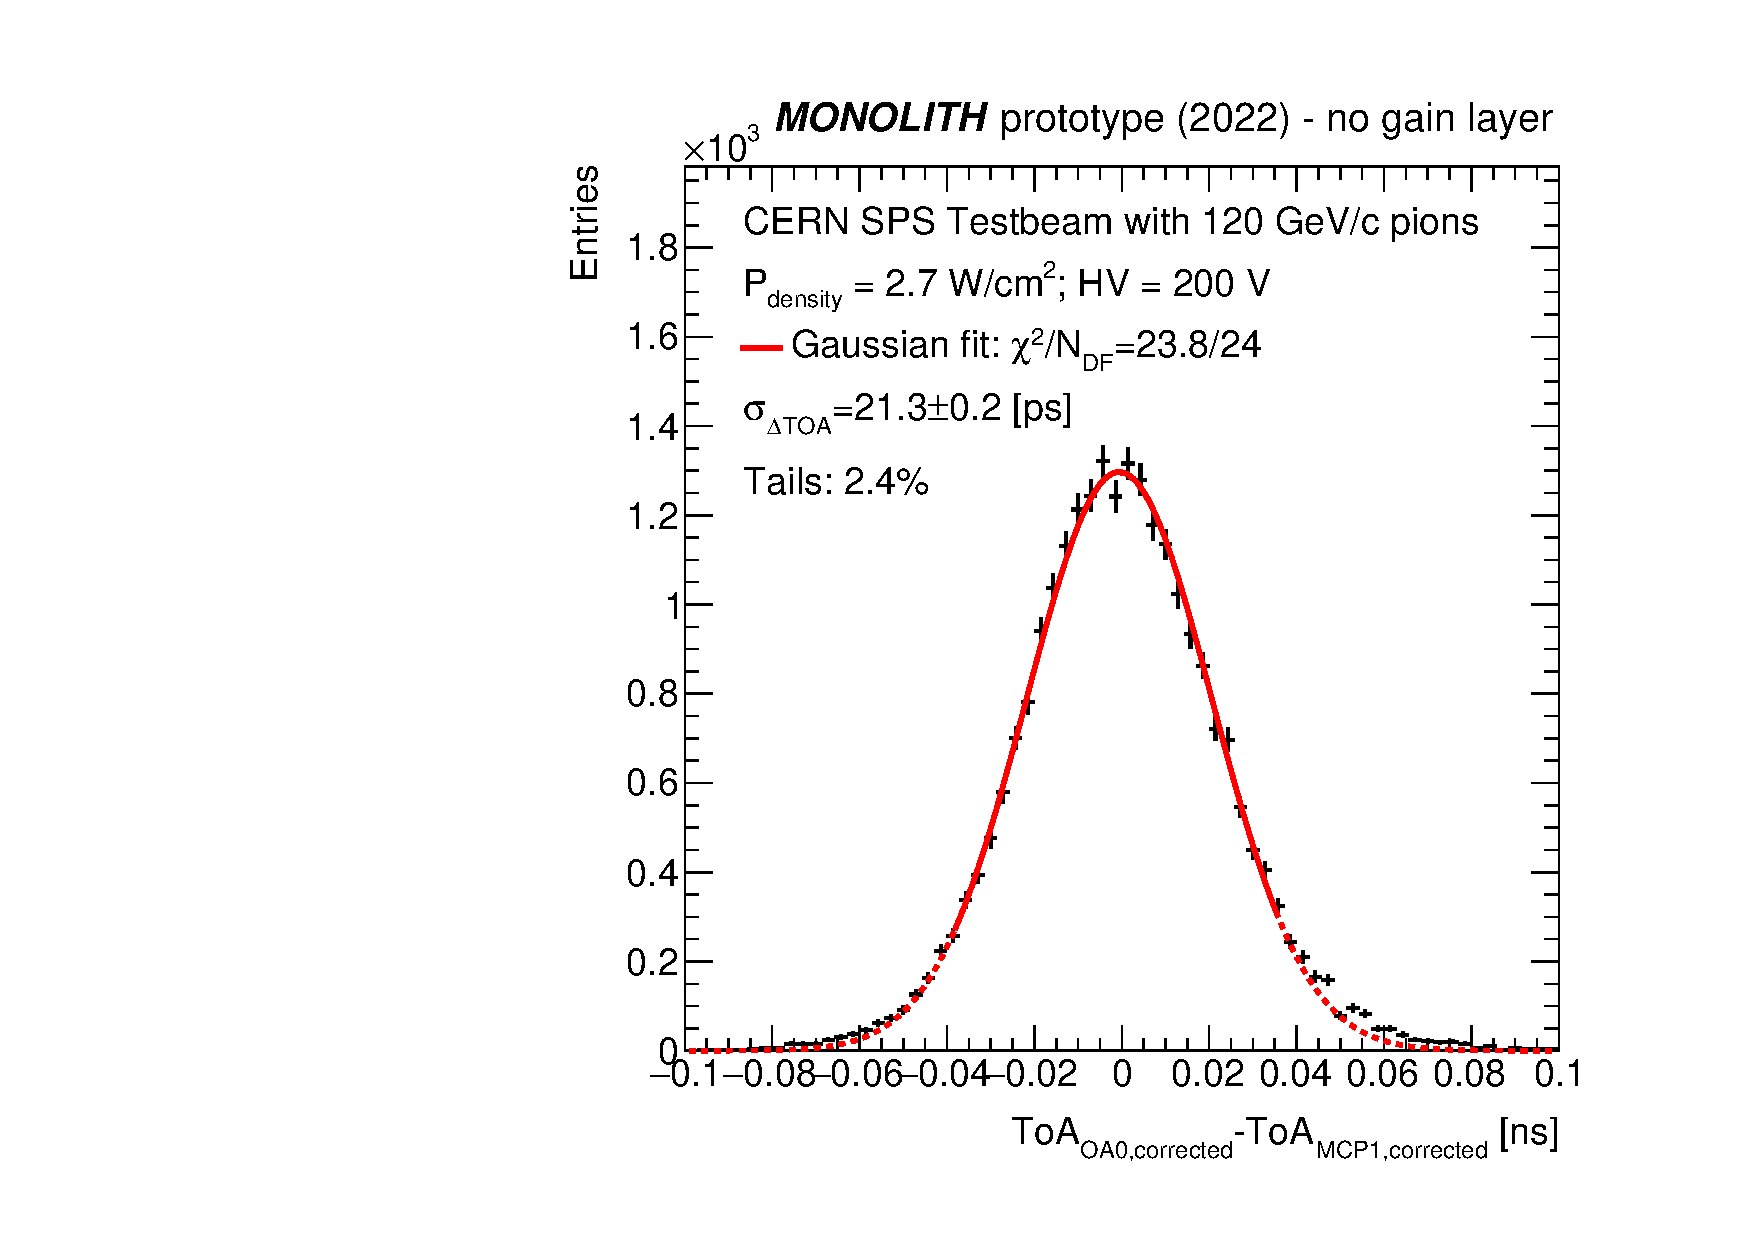
\includegraphics[width=.33\textwidth,trim=40 20 30 20]{files/MONOLITH_paper/TOF_2.pdf}
			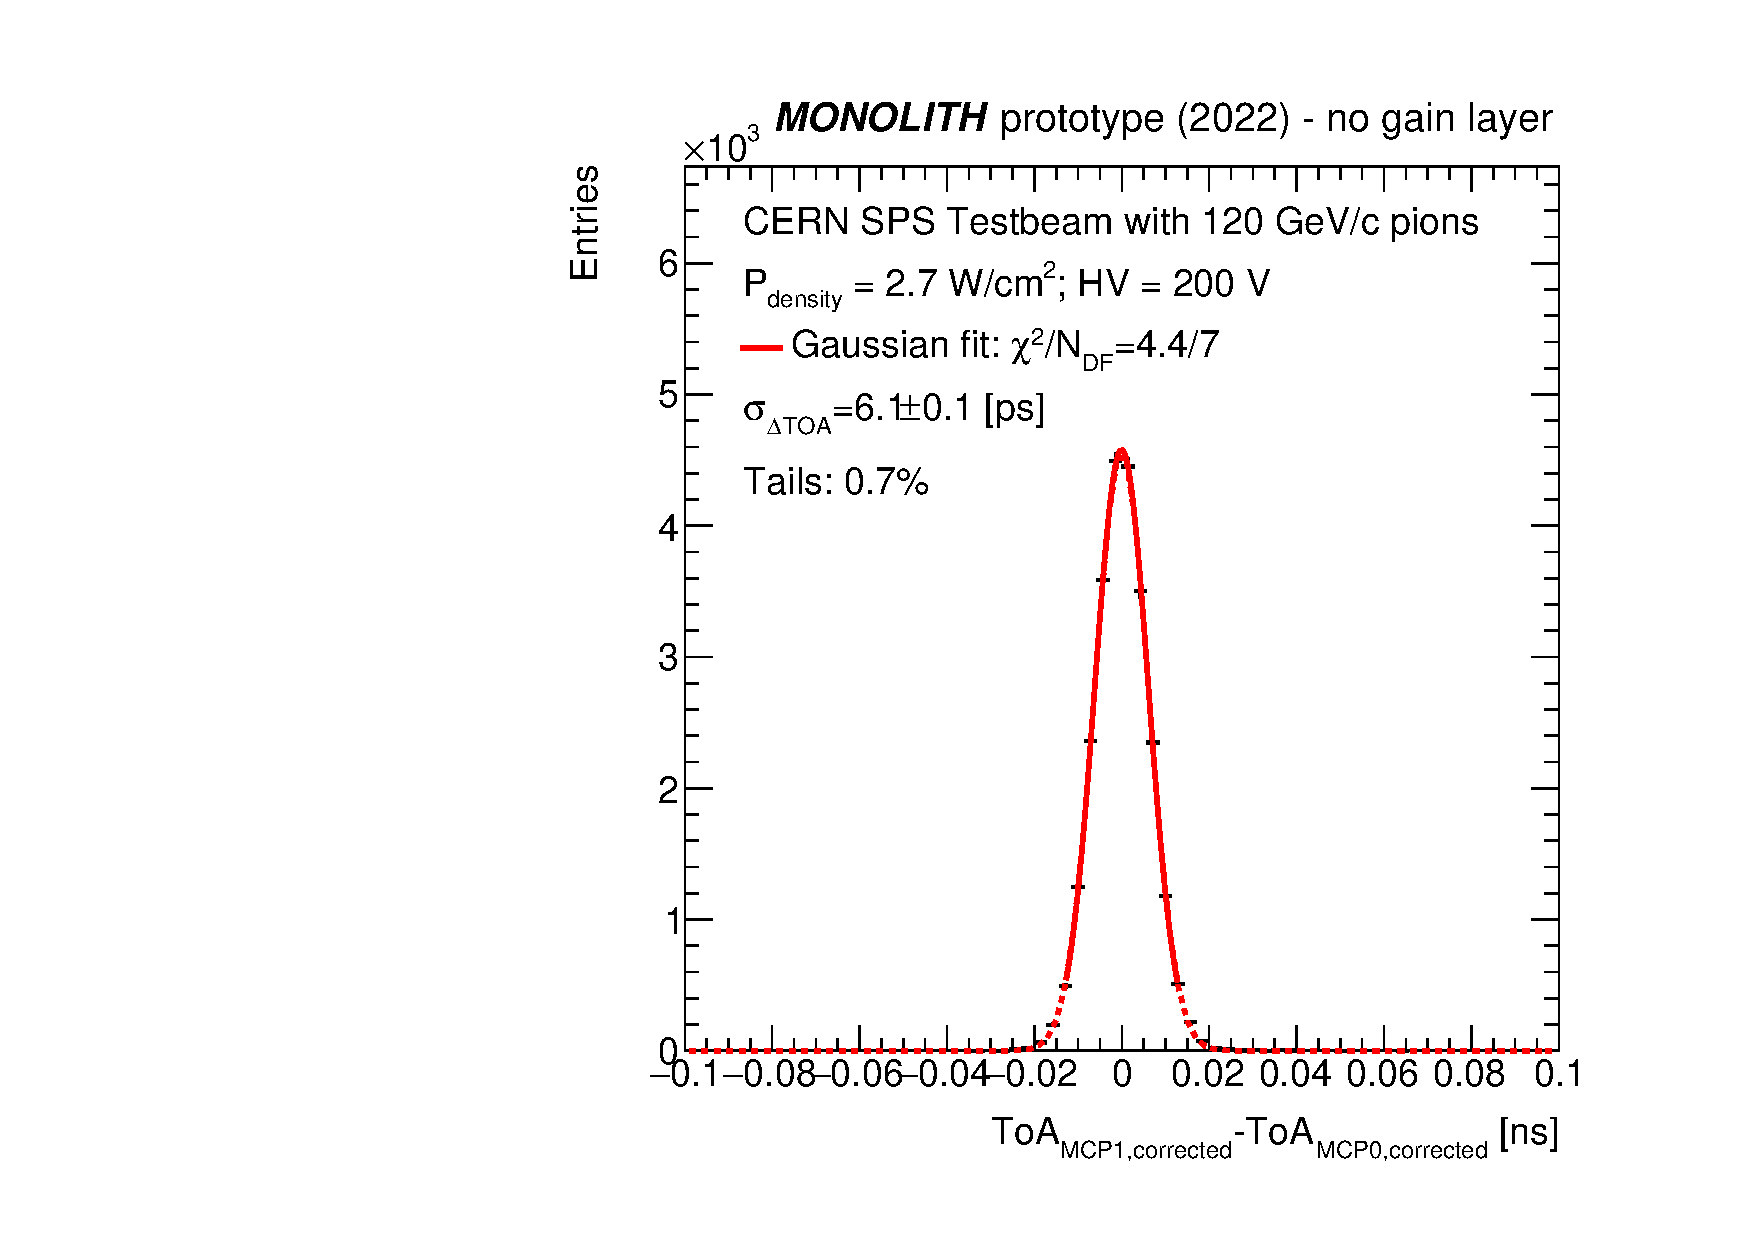
\includegraphics[width=.33\textwidth,trim=40 20 30 20]{files/MONOLITH_paper/TOF_3.pdf}
			\caption{Distributions of the time-walk-corrected \dtoa difference between the DUT and MCP0 (left), DUT and MCP1 (center), and between MCP0 and MCP1 (right), for the working point with power density of  \power = \SI{2.7}{\watt/\centi\meter^2} and $ HV =$ \SI{200}{\volt}. The full red lines show the results of the Gaussian fits to the bulk of each distribution, while the dashed lines extrapolate the fit to the entire histogram range. The non-Gaussian contributions in the tails are reported in the plots, as well as the three \sigdtoa used to calculate the DUT and MCPs time resolutions.}
			\label{im:MONO_TOF_fits} 
		\end{figure}

		As an example, the \dtoa distributions for the working point with power density of \power = \SI{2.7}{\watt/\centi\meter^2} and sensor bias voltage $ HV =$ \SI{200}{\volt} are shown in Figure \ref{im:MONO_TOF_fits}.
		A time resolution of $(20.7\pm 0.3)$ ps is measured for this working point. It was checked that, for the same working point, the time resolution is 48 ps without the correction for time walk.

		The very narrow distribution of the \dtoa between the two MCPs in Figure \ref{im:MONO_TOF_fits} indicates their excellent timing performance, measured to be ($3.6\pm1.5$) ps for MCP0 and ($5.0\pm1.1$) ps for MCP1, and confirms their ability to serve as a good time reference. 

		The total fraction of events exceeding the Gaussian-fit integral in the \dtoa distributions involving the DUT was found to be below 3\% for all the working points, showing that the non-Gaussian component of the time response of the \textit{MONOLITH} prototype is overall small and that the resolutions measured with this method describe at least 97\% of the recorded signals. 
		It was verified that these small non-Gaussian tails mainly originate from events with small amplitudes that are associated to pions crossing the DUT in the inter-pixel regions, for which pixel OA0 collected only a fraction of the charge produced.
		Extension of the time-resolution measurement to all events containing a hit in pixel OA0 (thus removing the request for the hit to be within the two triangles of Figure \ref{im:MONO_effmap}) does not change the time resolution values. The only effect produced is that the events with \dtoa outside the Gaussian fits increases from 3\% to 5\%; it was checked that these extra events in the tails are associated to hits in the inter-pixel region of the three sides of the OA0 pixel hexagon for which the adjacent pixels were not readout.


		Table \ref{tab:MONO_tabsumm} and the left panel of Figure \ref{im:MONO_TOF_power_HV} report the time resolution measured at  $HV =$ 200 V for the five power density values ranging from 0.04 to \SI{2.7}{\watt/\centi\meter^2}. 
		While the efficiency remains at the 99.8\% level in all cases, a gradual deterioration of the timing performance is visible at lower power density values, although it remarkably remains at the level of \SI{30}{\pico\second} at power density of 0.36 W/cm$^2$ and \SI{80}{\pico\second} at \SI{0.04}{\watt/\centi\meter^2}. 

		\begin{table}[h]
			\centering
			\renewcommand{\arraystretch}{1.2}
			\begin{tabular}{|c|c|c|}
			\cline{1-3}
			\multicolumn{3}{|c|}{DUT operated at  $ HV = \SI{200}{\volt} $ and $V_{\it th} = 7 \sigma_V$} \\ 
			\cline{1-3}
			~~\power [W/cm$^2$]~~ & Amplitude MPV [mV] & Time Resolution [ps] \\
			\cline{1-3}
			2.7   & $ 48.6 \pm 0.5 $ &   $20.7 \pm 0.3$ \\
			0.9   & $ 35.8 \pm 0.5 $ &   $23.8 \pm 0.3$ \\
			0.36  & $ 22.6 \pm 0.4 $ &   $30.1 \pm 0.4$ \\
			0.13  & $ 14.2 \pm 0.3 $ &   $47.2 \pm 0.7$ \\
			0.04  & $ 16.2 \pm 0.3 $ &   $77.1 \pm 0.9$ \\
			\cline{1-3}
			\end{tabular}
			\caption{ Time resolution at sensor bias voltage $HV =$ \SI{200}{\volt} for the five power densities. The measurements refer to the area of pixel OA0 that is inside the two triangles of Figure \ref{im:MONO_effmap}. The most probable values of the amplitude of the differential signals are also reported. The uncertainties are statistical only.}
			\label{tab:MONO_tabsumm} 
		\end{table}

		The right panel of Figure \ref{im:MONO_TOF_power_HV} shows the time resolution as a function of the sensor bias voltage for power density of \power = \SI{2.7}{\watt/\centi\meter^2}. The measurement show that the DUT can be operated in a wide $HV$ range with a time resolution between 20 and \SI{25}{\pico\second}.


		\begin{figure}[h]
			\centering %
			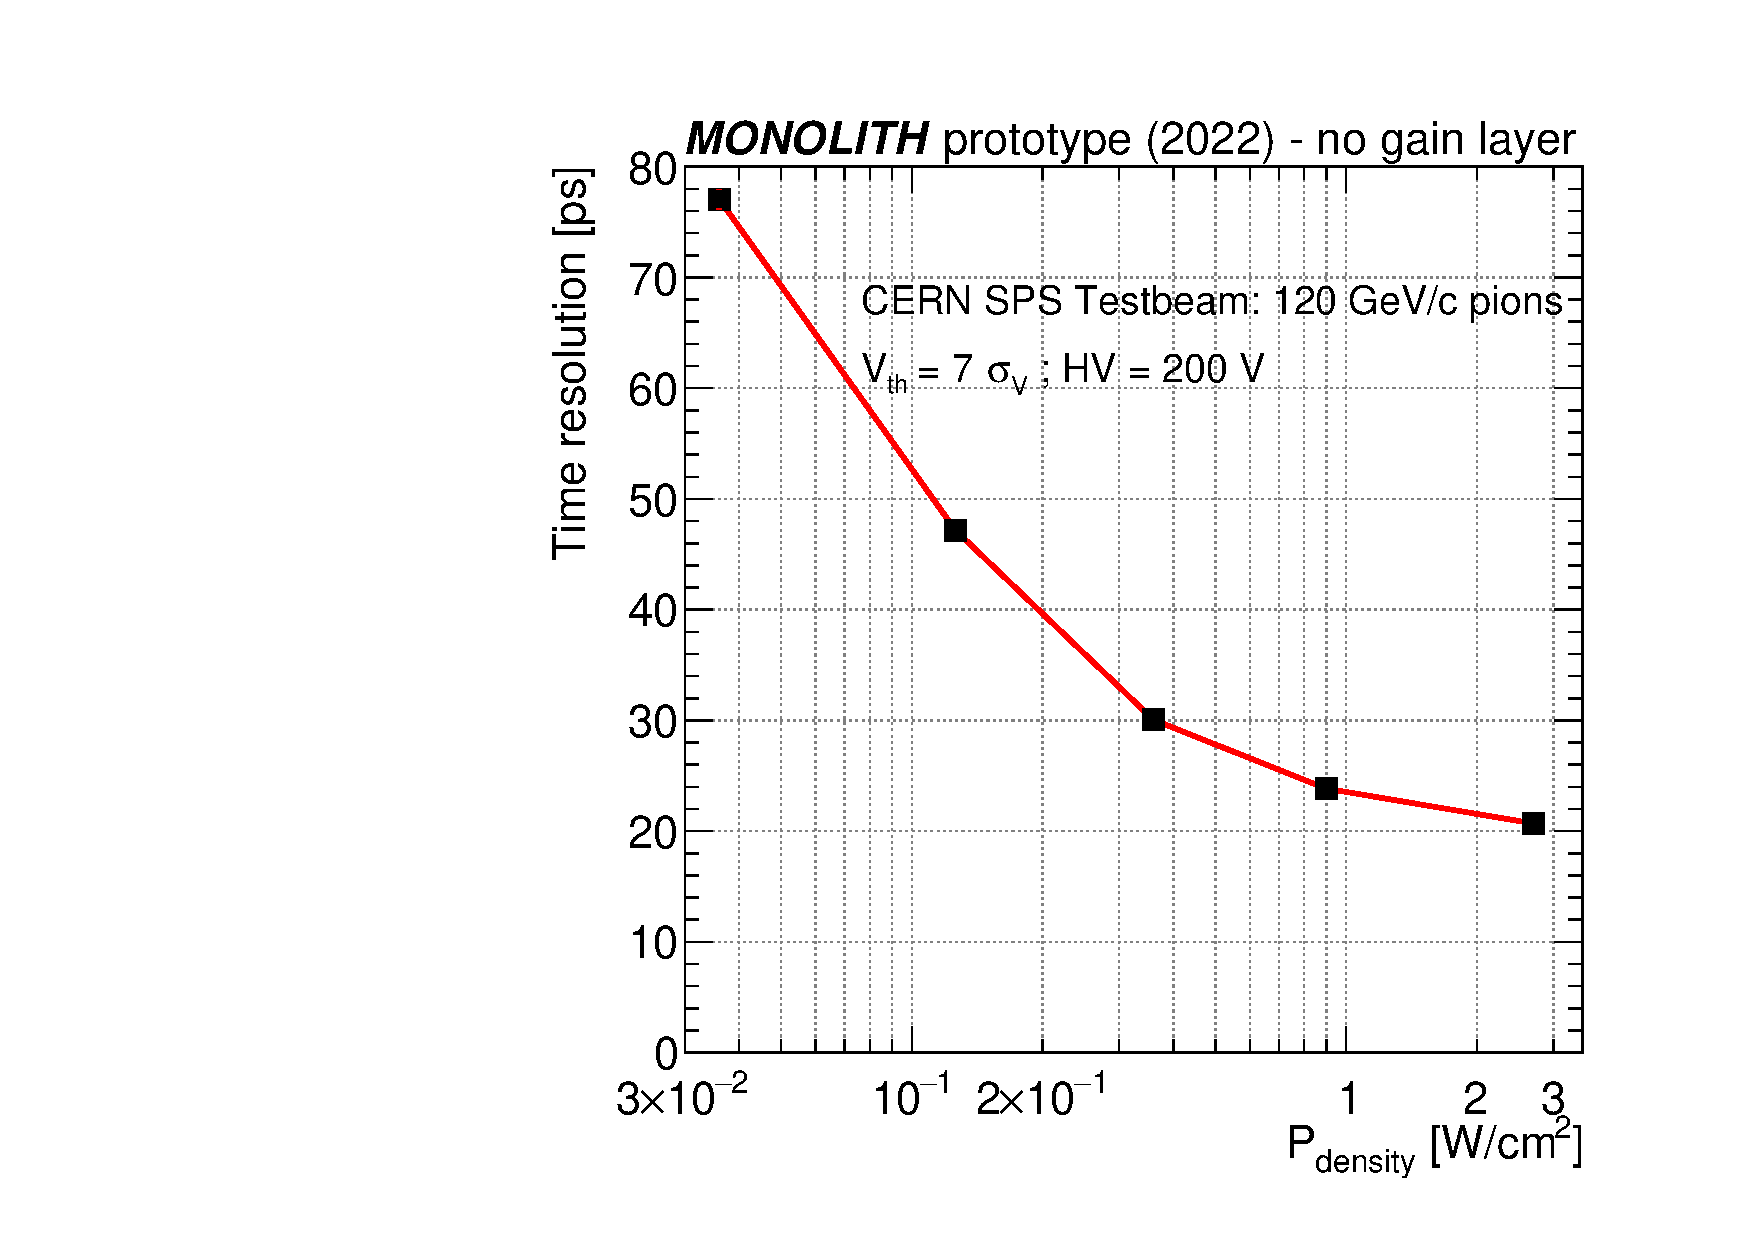
\includegraphics[width=.49\linewidth]{files/MONOLITH_paper/timeres_vs_power.pdf}
			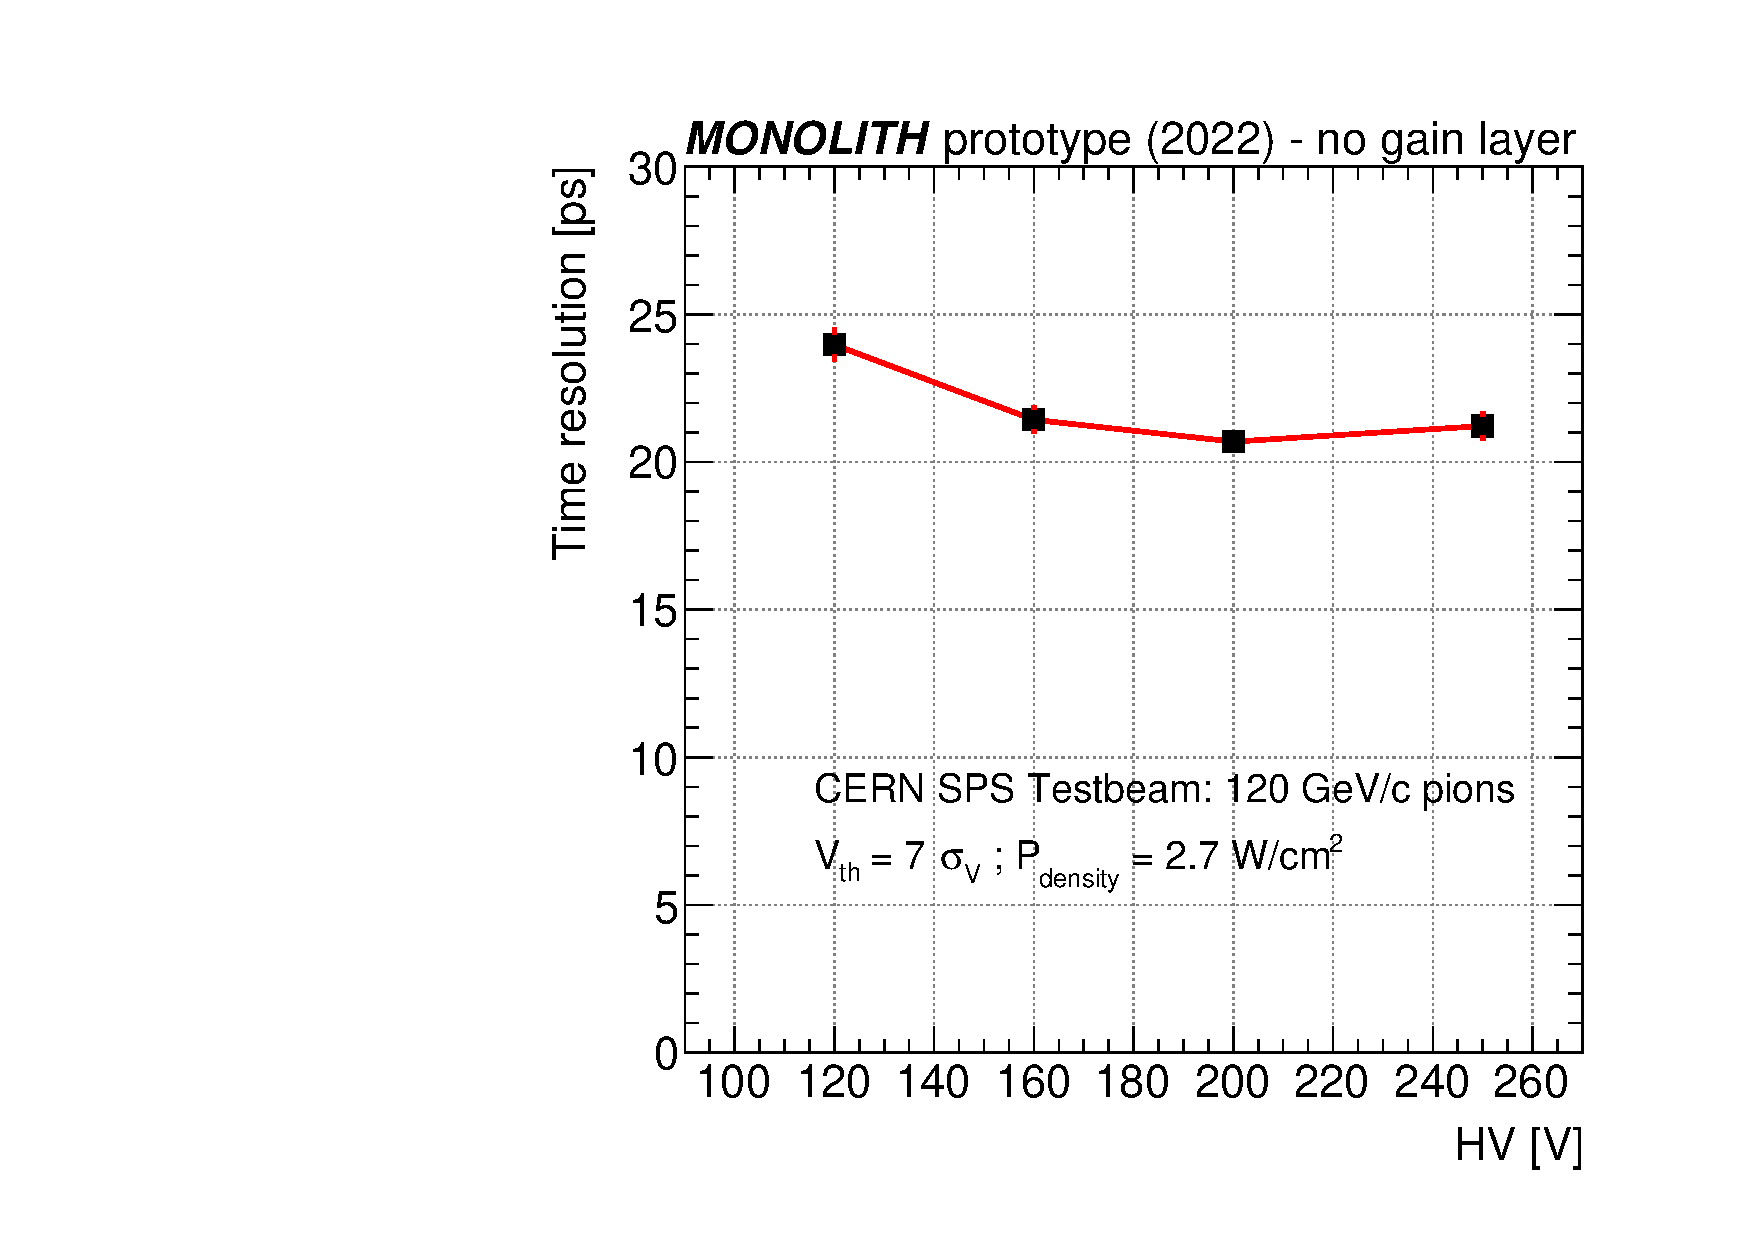
\includegraphics[width=.49\linewidth]{files/MONOLITH_paper/timeres_vs_HV.pdf}
			\caption{Time resolution measured for sensor bias voltage HV = 200 V as a function of the power density (left panel), and for power density of \power = \SI{2.7}{\watt/\centi\meter^2} as a function of sensor bias voltage (right panel).}
			\label{im:MONO_TOF_power_HV} 
		\end{figure}

		\begin{figure}[h]
			\centering %
			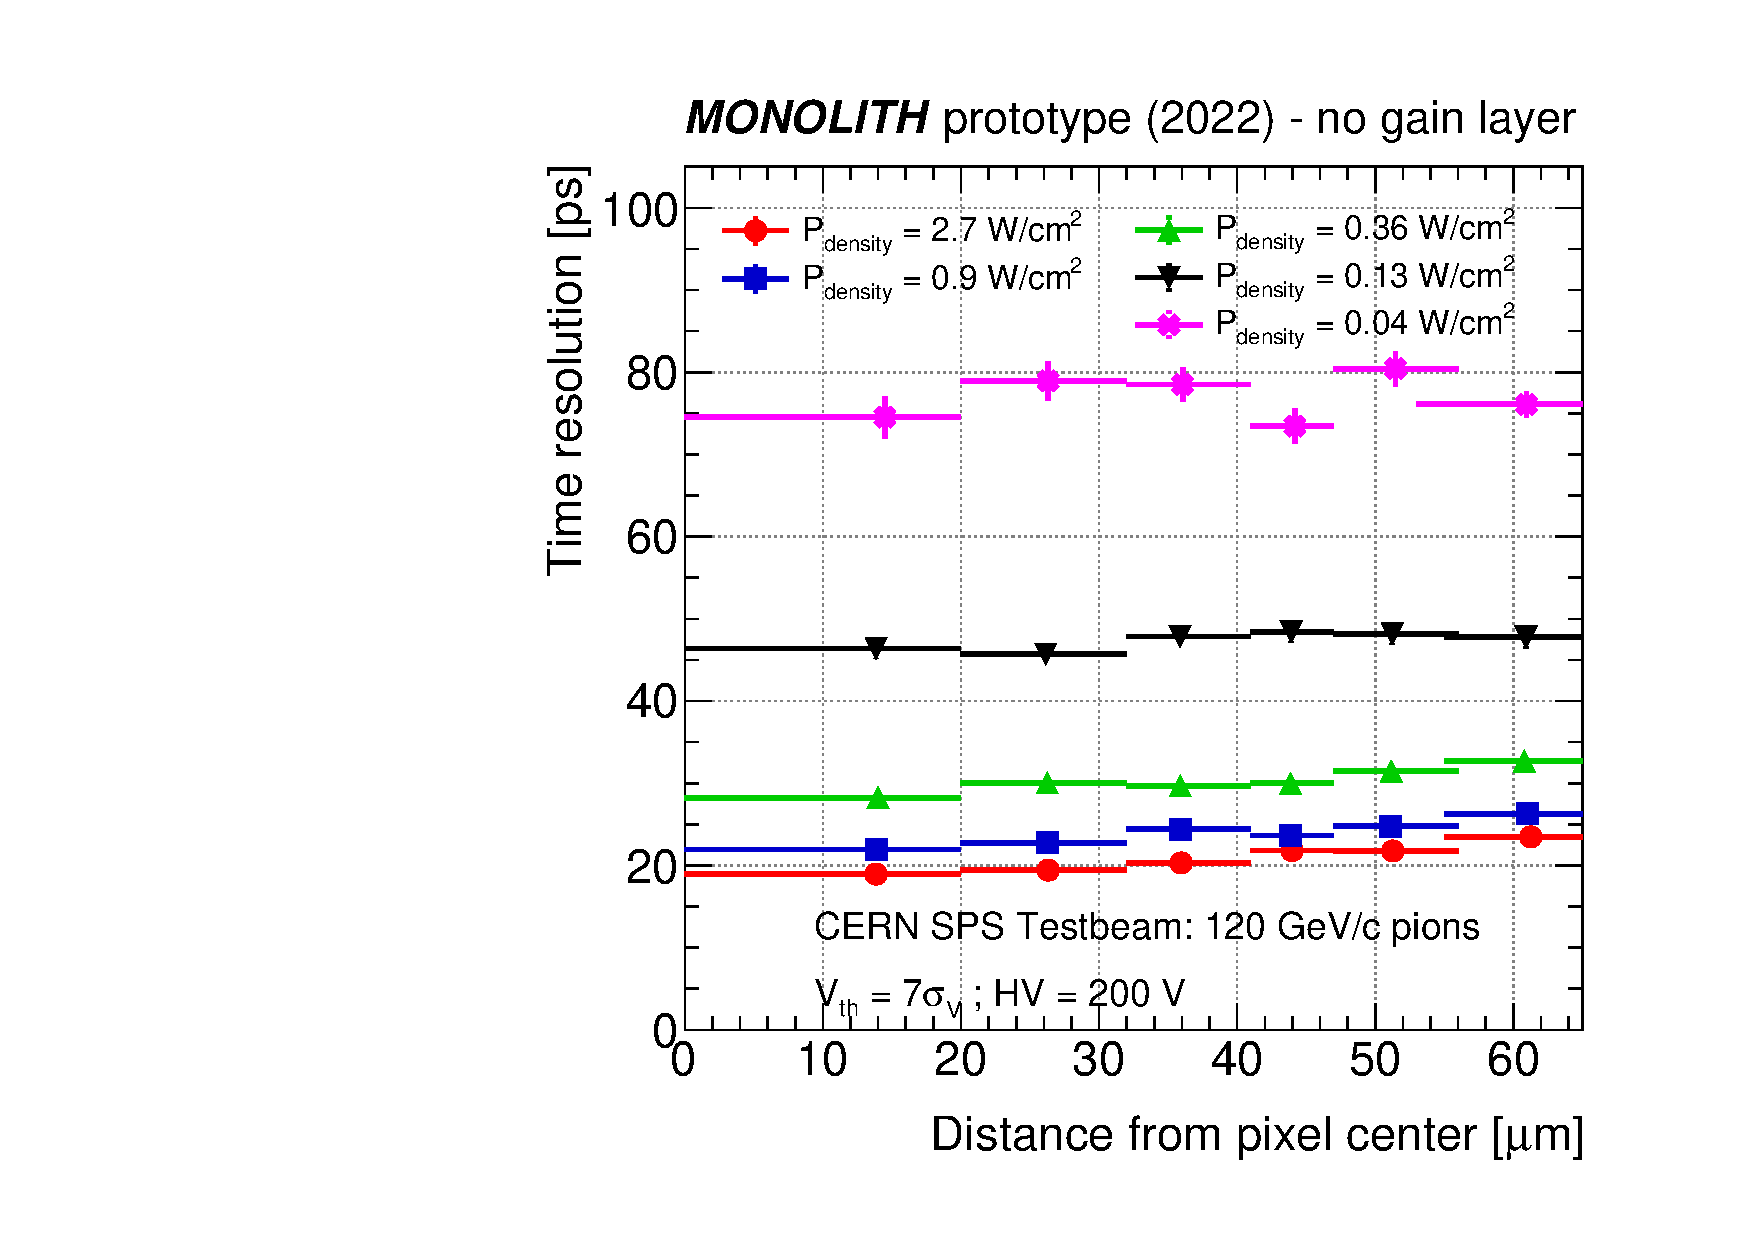
\includegraphics[width=.49\linewidth]{files/MONOLITH_paper/timeres_vs_radius_allWP.pdf}
			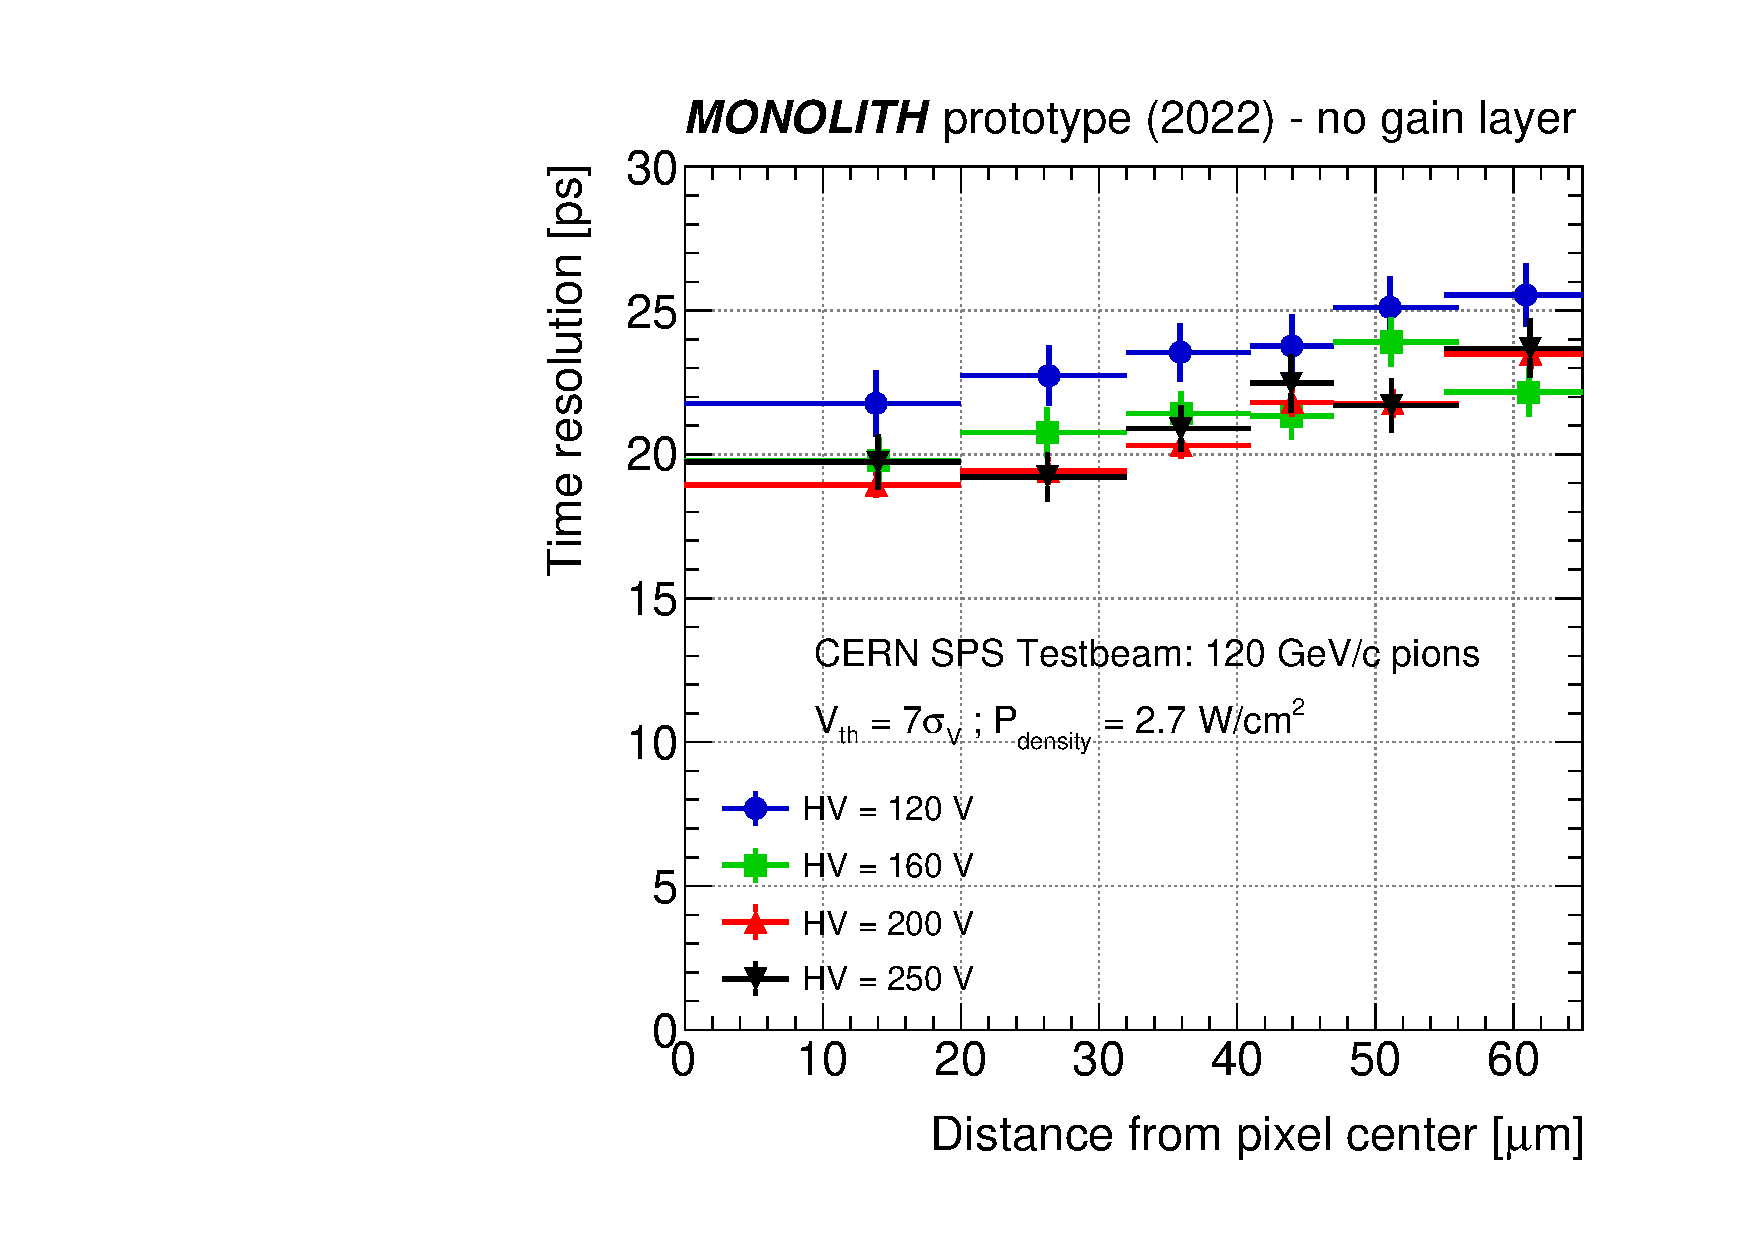
\includegraphics[width=.49\linewidth]{files/MONOLITH_paper/timeres_vs_radius_allHV.pdf}
			\caption{Time resolution as a function of the distance from center of the pixel OA0. In the left panel, the resolution is shown for the five power density values acquired at sensor bias voltage HV = 200 V. In the right panel, it is measured at a power density of \power = \SI{2.7}{\watt/\centi\meter^2} for the four sensor bias voltage values acquired. In each  bin the data point marker is placed at the average distance value from the pixel center.}
			\label{im:MONO_TOF_radius} 
		\end{figure}


		The time resolution was also measured as a function of the distance from the center of the pixel OA0. The left panel of Figure \ref{im:MONO_TOF_radius} shows that a mild dependence on the distance from the pixel center is measured only for \power $\ge$ \SI{0.36}{\watt/\centi\meter^2}, when the time resolution is below $\approx$30 ps. The right panel of the Figure shows that the time resolutions measured for $HV$ between 160 and 250 V are compatible with each other within uncertainties, while at $HV$ = 120 V the measurements are systematically higher by approximately 2 ps. This observation might hint that the charge drift velocity at $HV$ = 120 V is not yet saturated deep in the sensor volume.

		All the time resolution measurements are obtained with the \toa computed with a simple threshold setting (that offers the significant advantage of requiring a simple electronics circuitry) and a simple signal-processing method (linear interpolation between consecutive oscilloscope samplings).
		More complex signal-processing methods (mimicking a low-pass RC filter, a constant-fraction discriminator, or spline interpolation of the oscilloscope signal samplings), which would require a more complex electronics, improve marginally the time resolutions, at most at the 10\% level.















	\clearpage
	\section{Radiation Tolerance of \textit{MONOLITH} Prototypes}
	In early 2023, a collection of \textit{MONOLITH} prototypes were irradiated at the CYRIC facility \cite{CYRIC_facility} in Japan with \SI{70}{\mega\electronvolt} protons, up to a fluence of \maxflu. In July 2023, these ASICs were tested during a test beam campaign organised at the CERN SPS North Area experimental hall. The beam used to qualify the ASIC was composed of pions with a momentum of \SI{120}{\giga\electronvolt}/c a beam spread of about a few millimetres wide and very straight tracks (almost no beam divergence). The track position on the DUT were reconstructed using the FE-I4 UniGe telescope \cite{telescope} and allowed for a mesure of the detection efficiency and time resolution as a function of the particle position within the pixel. The set-up used was the same as the one described for the testbeam of the non-irradiated \textit{MONOLITH} prototypes with the addition of a thermal chamber, keeping the DUT at low temperatures in order to avoid unwanted annealing. A first characterisation in the laboratory of the prototypes was published in \cite{LabRad_Mono2023}.
		
	The results are presented for the prototypes as a function of the power density (\power), as a function of the High Voltage (HV) bias given to the substrate and as a function of the particle's position within the pixel and are compared with the non-irradiated samples. The following section refers to the work published in June 2024 in the Journal of Instrumentation (JINST) \cite{Moretti_irradiated}.

		\subsection{Data samples and experimental set-up}
		Given the limited time availability during the testbeam experiment, data were taken only with four irradiated boards out of the seven characterised in \cite{LabRad_Mono2023}. 
		In addition, data were taken also with the board not irradiated previously characterised in \cite{Monolith_20ps}.
		Table \ref{tab:MONO-IR_wp} gives a summary of the power density of the frontend and of the sensor bias voltage of the 18 datasets taken at the testbeam. All boards were operated at a frontend feedback current of 2.0 $\mu$A and, to avoid any unwanted annealing, stored and operated at a temperature of -10 $^\circ$C. 

		\begin{table}[h]
			\centering
			\renewcommand{\arraystretch}{1.3}
			\begin{tabular}{|c|ccc|cccc|}
			\cline{1-8}
			\begin{tabular}{c} Proton Fluence \\ \ [1 MeV n$_{\text{eq}}$/cm$^2$] \end{tabular} & \multicolumn{3}{c|}{\power~ [W/cm$^2$]}  & \multicolumn{4}{c|}{High Voltage [V]} \\
			\cline{1-8}
			0                   & 0.13 & 0.54 & 0.9                                   & \multicolumn{4}{c|}{\multirow{4}{*}{200}} \\ \cline{1-4}
			$9 \times 10^{13}$  & 0.13 & 0.54 & 0.9                                   & \multicolumn{4}{c|}{} \\ \cline{1-4}
			$6 \times 10^{14}$  & 0.13 & 0.54 & 0.9                                   & \multicolumn{4}{c|}{} \\ \cline{1-4}
			$3 \times 10^{15}$  & 0.13 & 0.54 & 0.9                                   & \multicolumn{4}{c|}{} \\ \hline
			\multirow{2}{*}{$1 \times 10^{16}$ } & \multicolumn{3}{c|}{\begin{tabular}{cc}  0.13  & 0.54 \end{tabular}} & \multicolumn{4}{c|}{250} \\ \cline{2-8}
			& \multicolumn{3}{c|}{0.9} & 150 & 200 & 250 & 300 \\
			\cline{1-8} 
			\end{tabular}
			\caption{ Power density and sensor bias voltage of the 18 data samples taken at the CERN SPS testbeam with the four irradiated boards and with the board not irradiated. The proton-fluence values  are reported in the first column in 1 MeV \flu~values.}
			\label{tab:MONO-IR_wp} 
		\end{table}

		The UNIGE FE-I4 telescope \cite{telescope} was used to provide external tracking. The DUT was mounted at the center of the telescope as explained in \cite{Monolith_20ps}.
		Two MCPs were positioned downstream of the telescope and used as time reference.
		The analog outputs of the two MCP detectors and of the DUT were read by two fast oscilloscopes. The first one with a sampling rate of 20 GS/s and an analog bandwidth set to 4 GHz for the channels connected to the MCPs and 1 GHz for the channels connected to the pair of single-ended analog output of the pixel used to measure the DUT time resolution. Two other pairs of single-ended output of adjacent pixels were connected to the second oscilloscope with a sampling rate of 10 GS/s and an analog bandwidth set to 1 GHz.
		The DUT was mounted on a cooling plate and covered by an insulating box to keep the ASIC at a constant temperature of -10 $^\circ$C. 

		The waveforms acquired for the positive and negative single-ended signals of the DUT were subtracted offline, sample point by sample point, to construct differential signals. Throughout the analysis, only the differential signals were used since they provide better signal-to-noise ratio. 


		\subsection{Detection efficiency}
		The detection efficiency was computed using pion tracks reconstructed by the FE-I4 telescope that produced hits in the six telescope planes and with a $\chi^2$/NDF $\le$ 1.5.

		Since the number of channels available in the two oscilloscopes allowed recording of the signals from only two out of six neighbouring analog pixels, the calculation of the efficiency was restricted to the telescope tracks whose extrapolation on the pixel surface was inside the region defined by the triangle connecting the center of the three pixels (the pixel under study and the two adjacent pixels that were read out).
		\begin{figure}[h]
			\centering
			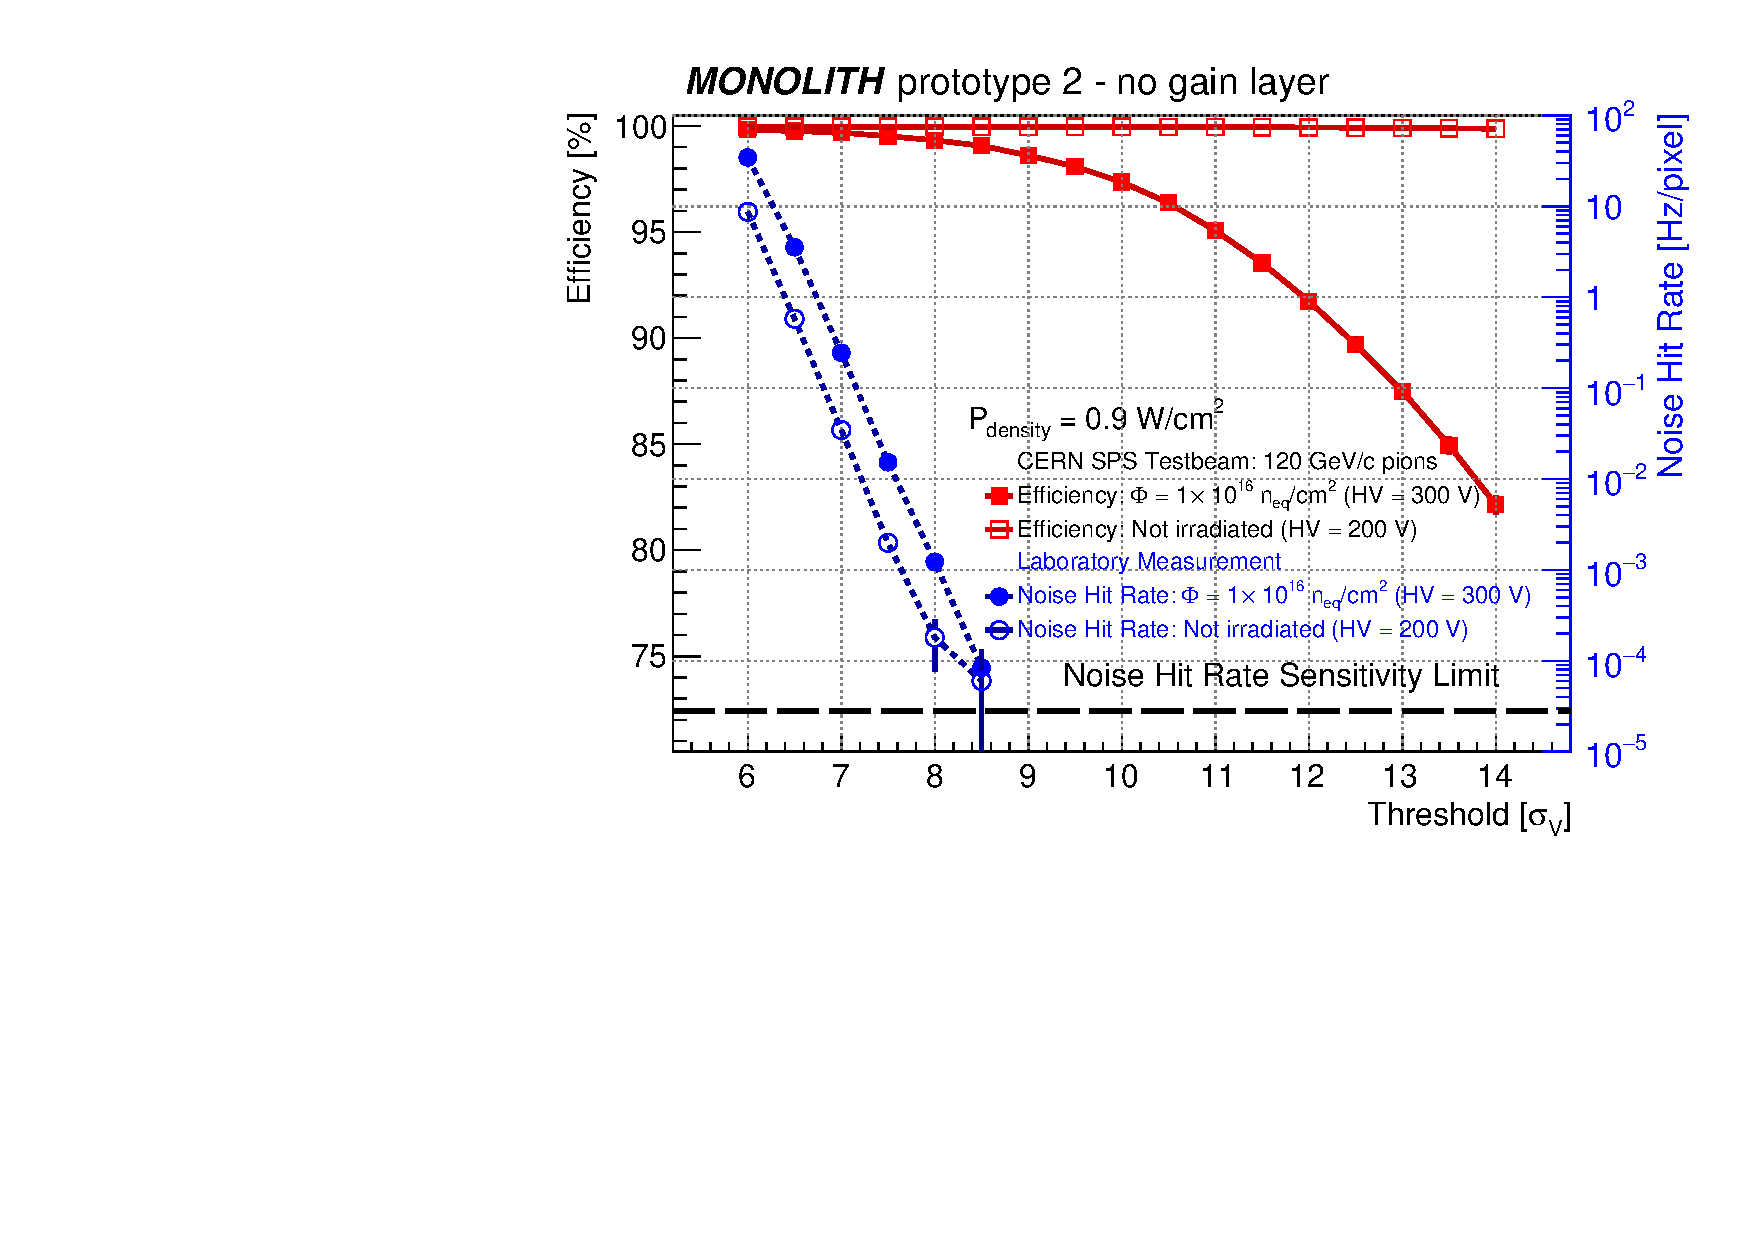
\includegraphics[width=.85\textwidth]{files/MONOLITH_Irradiated_paper/M06_M16}
			\caption{Detection efficiency measured at a power density \power~= 0.9 W/cm$^2$ as a function of the voltage threshold. The data refer to the board not irradiated operated at HV = 200 V (open red squares), and to the board irradiated at \maxflu~operated at HV = 300 V (full red squares). The voltage threshold is given in units of the voltage noise \noise, which is \SI{300}{\micro\volt} before irradiation and raises to \SI{600}{\micro\volt} after a fluence of \maxflu, as reported in~\cite{LabRad_Mono2023}. The plot reports also the noise-hit rate (values reported on the right-hand-axis scale) measured with the two boards.}
			\label{im:MONO-IR_HV_vs_th} 
		\end{figure}
		
		Figure~\ref{im:MONO-IR_HV_vs_th} shows the efficiency as a function of the voltage noise \noise, in the case of the board not irradiated operated at a sensor bias voltage of 200 V, and of the board irradiated at \maxflu~operated at 300 V. 
		The increase of HV for the irradiated board was necessary to fully deplete the sensor and operate it at very high efficiency after the change in resistivity due to the exposure to radiation.
		The voltage noise \noise was measured event-by-event using the waveform samplings recorded in a time interval of 200 ns preceding the signal.
		At the nominal threshold value \vth~= 7 \noise, the ASIC not irradiated provides a detection efficiency of (99.96$^{~\!+0.01}_{-0.02}$)\% and, given the large signal-to-noise ratio, it maintains an efficiency at the level of 99.8\% even with a threshold value of 14 \noise.
		On the contrary, in the case of the ASIC that was exposed to \maxflu, since the signal-to-noise ratio diminishes, the efficiency was found to depend more on the threshold, and at HV = 300 V varies from 99.7\% at a threshold \vth~= 7 \noise to approximately 97.0\% already at \vth = 10 \noise. 
		Figure \ref{im:MONO-IR_HV_vs_th} also reports the noise-hit rate as a function of the threshold. The noise-hit rate shows the expected exponential drop. It increases by a factor of approximately five after the ASIC has received a proton fluence of \maxflu.
		\begin{figure}[h]
			\centering
			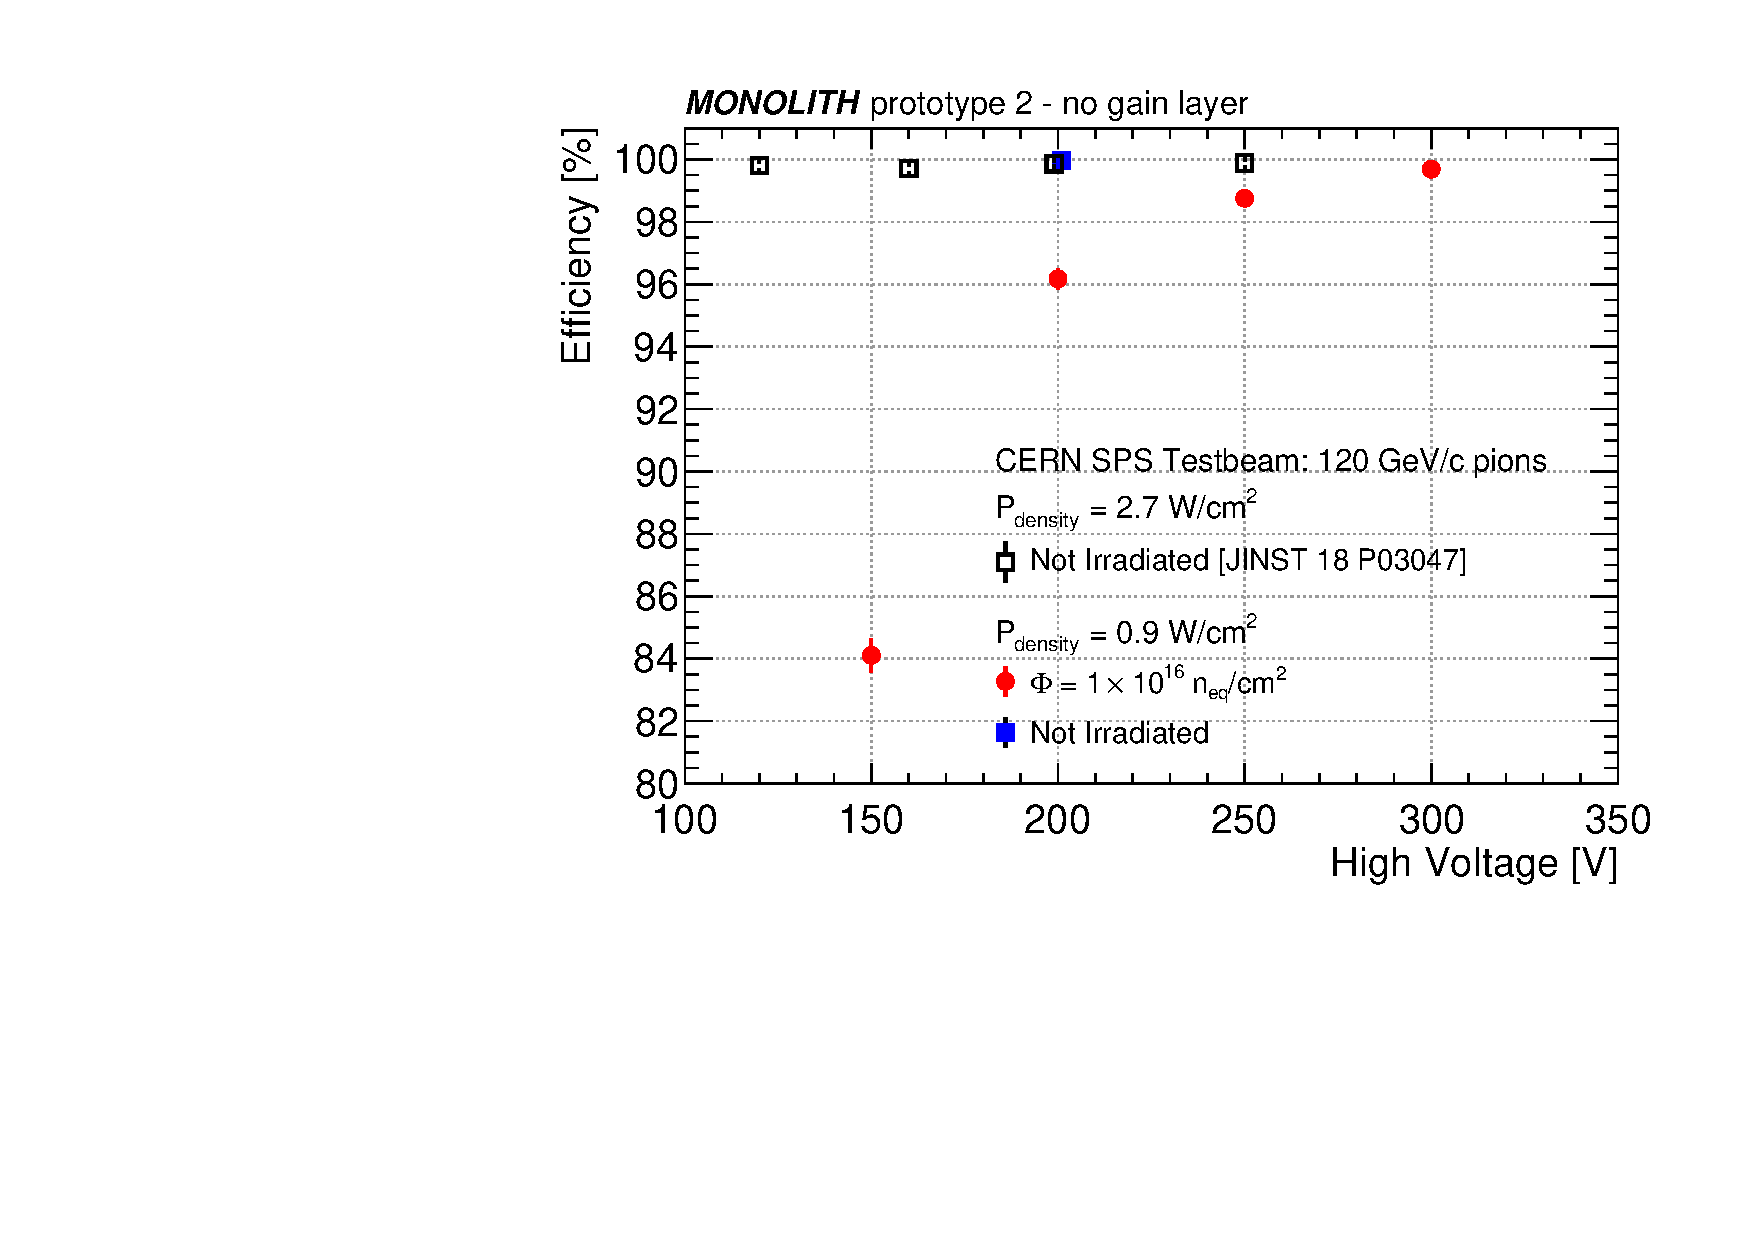
\includegraphics[width=.75\textwidth]{files/MONOLITH_Irradiated_paper/Voltage_efficiency}
			\caption{Detection efficiency measured as a function of the sensor bias voltage at a threshold value \vth~= 7 \noise. The red dots show the results obtained with the board irradiated at \maxflu, while the blue square that obtained with the board not irradiated, all  operated at \power~= 0.9 W/cm$^2$. The results obtained with the board not irradiated at \power~= 2.7 W/cm$^2$ reported in \cite{Monolith_20ps} are superimposed as black open squares.}
			\label{im:MONO-IR_HV_vs_eff} 
		\end{figure}




		\begin{table}[h]
			\centering
			\renewcommand{\arraystretch}{1.3}
			\begin{tabular}{|c|c|c|c|c|}
			\cline{1-5}
			\cline{1-5}
			\cline{1-5}
			\begin{tabular}{c} Proton Fluence \\ \ [1 MeV n$_{\text{eq}}$/cm$^2$] \end{tabular} & \begin{tabular}{c}\power~ \\ \ [W/cm$^2$] \end{tabular} & \begin{tabular}{c} High \\ Voltage \\ \ [V] \end{tabular} & \begin{tabular}{c}Detection \\ Efficiency \\ \ [\%]\end{tabular} & \begin{tabular}{c}Time \\ Resolution \\  \ [ps]\end{tabular} \\
			\cline{1-5}
			\multirow{3}{*}{ 0 }                    & 0.13 & \multirow{3}{*}{200}   & 99.94$^{~\!+0.03}_{-0.05}$ & 31.0 $\pm$ 1.6\\ \cline{2-2} \cline{4-5}
            			                            & 0.54 &                        & 99.96$^{~\!+0.02}_{-0.03}$ & 29.0 $\pm$ 1.3\\ \cline{2-2} \cline{4-5}
			                                        & 0.9  &                        & 99.96$^{~\!+0.01}_{-0.02}$ & 20.0 $\pm$ 1.0\\ \cline{1-5}
			\multirow{3}{*}{ $9 \times 10^{13}$ }   & 0.13 & \multirow{3}{*}{200}   & 99.12$^{~\!+0.10}_{-0.19}$ & 37.8 $\pm$ 2.8\\ \cline{2-2} \cline{4-5}
			                                        & 0.54 &                        & 99.63$^{~\!+0.07}_{-0.13}$ & 29.0 $\pm$ 1.3\\ \cline{2-2} \cline{4-5}
			                                        & 0.9  &                        & 99.78$^{~\!+0.04}_{-0.11}$ & 24.7 $\pm$ 1.0\\ \cline{1-5} 
			\multirow{3}{*}{ $6 \times 10^{14}$ }   & 0.13 & \multirow{3}{*}{200}   & 98.38$^{~\!+0.17}_{-0.19}$ & 42.4 $\pm$ 3.0\\ \cline{2-2} \cline{4-5}
			                                        & 0.54 &                        & 99.13$^{~\!+0.12}_{-0.13}$ & 29.9 $\pm$ 2.2\\ \cline{2-2} \cline{4-5}
			                                        & 0.9  &                        & 99.24$^{~\!+0.10}_{-0.11}$ & 26.4 $\pm$ 1.5\\ \cline{1-5} 
			\multirow{3}{*}{ $3 \times 10^{15}$ }   & 0.13 & \multirow{3}{*}{200}   & 94.06$^{~\!+0.22}_{-0.23}$ & 75.9 $\pm$ 4.5\\ \cline{2-2} \cline{4-5}
			                                        & 0.54 &                        & 97.22$^{~\!+0.17}_{-0.18}$ & 59.4 $\pm$ 0.9\\ \cline{2-2} \cline{4-5}
			                                        & 0.9  &                        & 97.97$^{~\!+0.11}_{-0.11}$ & 48.3 $\pm$ 1.9\\ \cline{1-5} 
			\multirow{6}{*}{ $1 \times 10^{16}$ }   & 0.13 & \multirow{2}{*}{250}   & 94.74$^{~\!+0.18}_{-0.19}$ & 74.0 $\pm$ 5.4\\ \cline{2-2} \cline{4-5}
			                                        & 0.54 &                        & 98.33$^{~\!+0.10}_{-0.11}$ & 48.3 $\pm$ 1.9\\ \cline{2-5}
			                    & \multirow{4}{*}{0.9}     & 150                    & 84.11$^{~\!+0.53}_{-0.54}$ & 60.4 $\pm$ 3.3\\ \cline{3-5} 
 			                                        &      & 200                    & 96.18$^{~\!+0.31}_{-0.33}$ & 53.1 $\pm$ 3.4\\ \cline{3-5}
                                        				&      & 250                    & 98.75$^{~\!+0.09}_{-0.10}$ & 50.2 $\pm$ 1.6\\ \cline{3-5}
                                       				&      & 300                    & 99.69$^{~\!+0.06}_{-0.07}$ & 45.3 $\pm$ 1.6\\ \cline{1-5}

			\end{tabular}
			\caption{Detection efficiency and time resolution measured for the 18 data samples taken at the CERN SPS testbeam with the four irradiated boards and with the board not irradiated. The values were obtained for a signal amplitude threshold \vth~> 7~\noise. }
			\label{tab:MONO-IR_effres} 
		\end{table}

		Table~\ref{tab:MONO-IR_effres} reports the detection efficiencies obtained at a threshold \vth~= 7 \noise for the 18 datasets listed in table \ref{tab:MONO-IR_wp}.  

		Figure \ref{im:MONO-IR_HV_vs_eff} shows the detection efficiency of the ASIC irradiated at \maxflu as a function of the sensor bias voltage. 
		Only one data set at HV = 200 V was acquired at the testbeam with the board not irradiated. The data taken with the board not irradiated in a previous testbeam \cite{Monolith_20ps} are superimposed in figure \ref{im:MONO-IR_HV_vs_eff} as open black squares for comparison. It should be noted that, in addition to the different power density, the data from \cite{Monolith_20ps} were acquired at feedback current $i_{\it feedback}$ = 0.1 $\mu$A and at a temperature of 20$^\circ$C in contrast with the 2.0 $\mu$A and -10$^\circ$C of the present data. This change in operating conditions results in an increase of the signal-to-noise ratio, that leads to better efficiency and time resolution.
		The measurement shows that after \maxflu a bias voltage of 300 V is just enough to reach the detection efficiency plateau. This behaviour is completely different from that of the non-irradiated board, for which the efficiency plateau is reached already at HV = 120 V.

		This measurement, as well as the drop in detection efficiency shown in figure \ref{im:MONO-IR_HV_vs_th}, could in large part be attributed to the change in resistivity of the silicon bulk, that we estimated to vary from the initial 350 $\Omega$cm to approximately 50 $\Omega$cm extrapolating the data of \cite{RadiationDamageBruzzi, DisplacementDamageMoll}.
		At such resistivity, the 50 $\mu$m thick sensor would not be fully depleted.
		A concurrent radiation damage of the frontend electronics cannot be excluded, and should be measured irradiating the SiGe HBT alone.


		\begin{figure}[h]
			\centering
			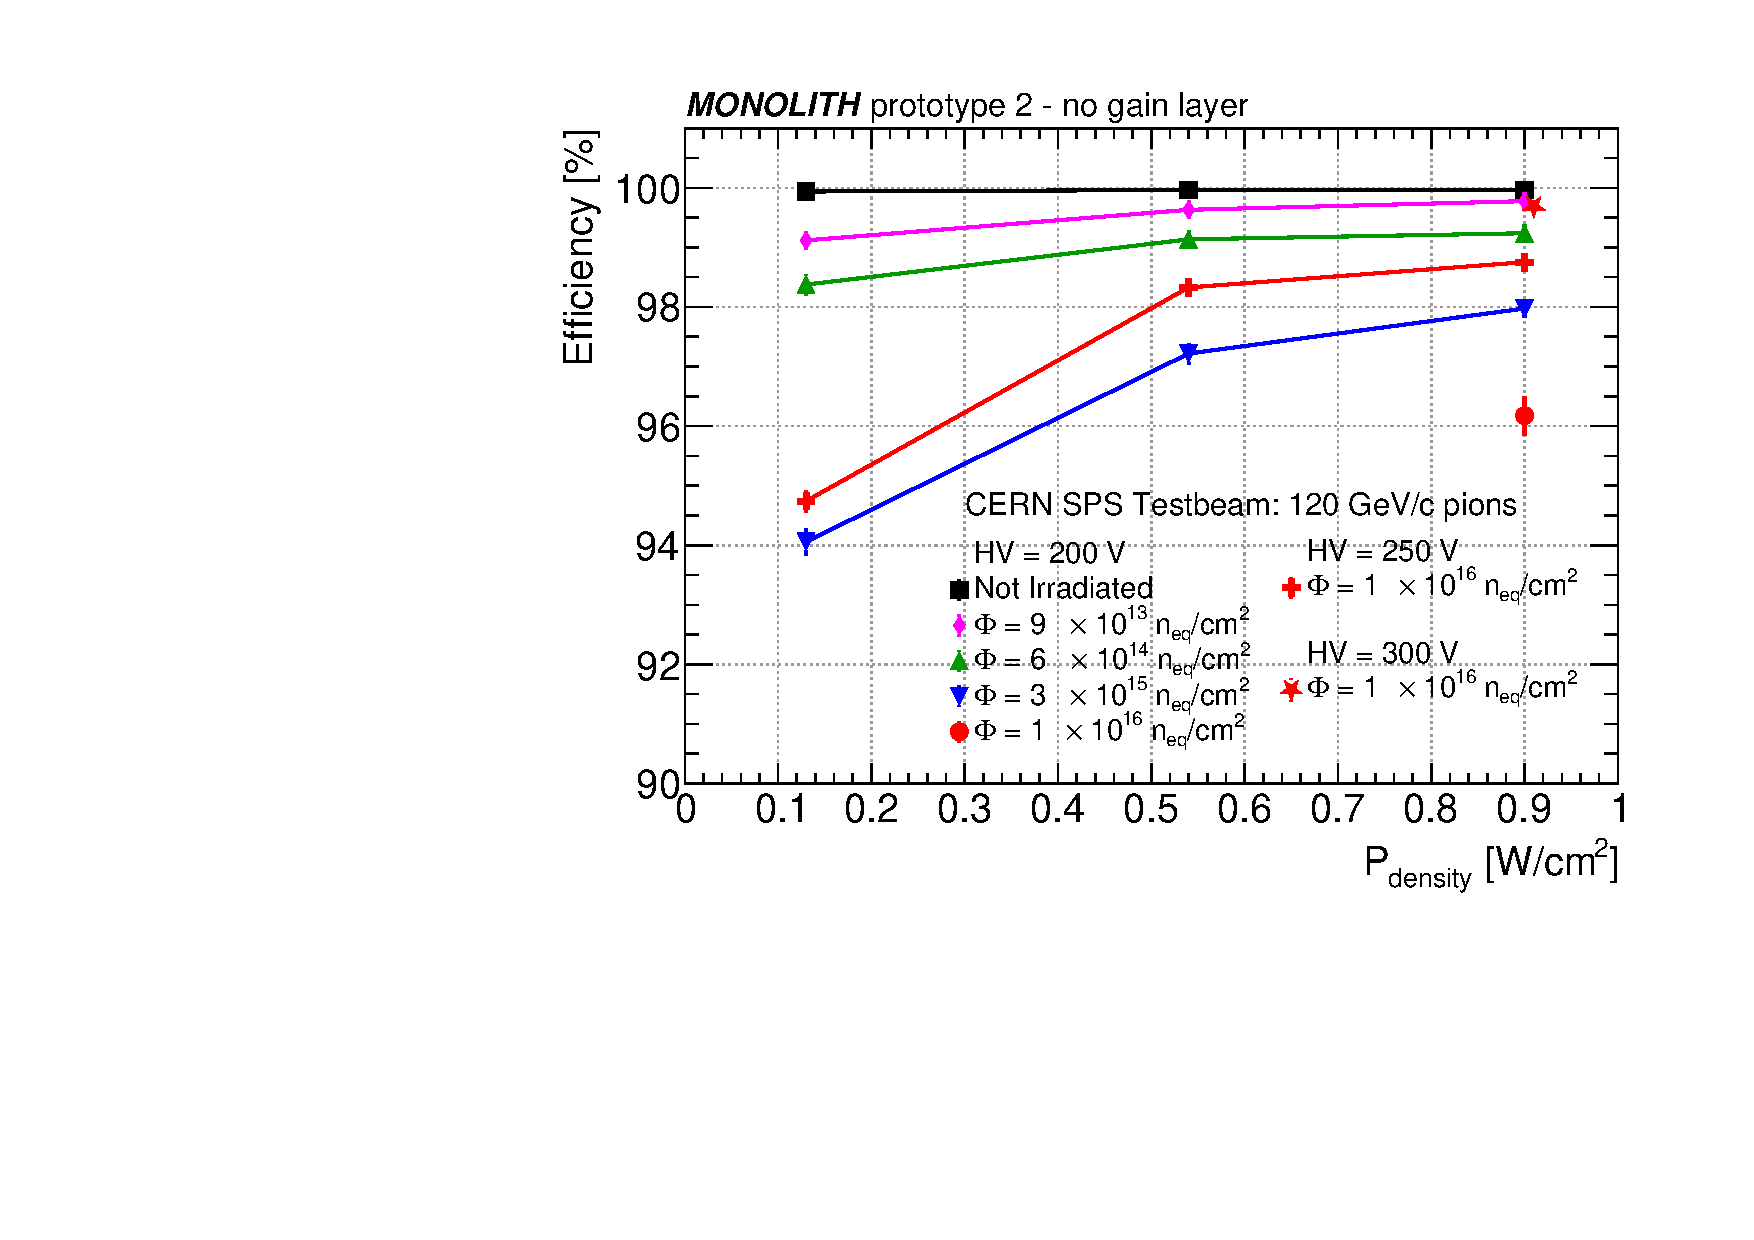
\includegraphics[width=.75\textwidth]{files/MONOLITH_Irradiated_paper/Power_efficiency}
			\caption{Detection efficiency measured for power density supplied to the preamplifier   between 0.13 and 0.9 W/cm$^2$ for a threshold value of \vth~= 7 \noise. The results obtained with the sample  not irradiated  (black empty squares) are presented with those of the four samples irradiated with fluences between $9 \times 10^{13}$ \flu  and $1 \times 10^{16}$ \flu, all operated with a sensor bias voltage of HV = 200 V. In the case of the board irradiated at \maxflu~the data taken at sensor bias voltage of 250 and 300 V are also shown. The marker relative to the data point at HV = 300 V (red star) is displayed with a small horizontal offset to avoid  overlapping with other markers.}
			\label{im:MONO-IR_Power_vs_eff}
		\end{figure}

		Figure \ref{im:MONO-IR_Power_vs_eff} shows the impact on the detection efficiency of the power density at which the frontend was operated. 
		At a sensor bias voltage HV= 200 V, a steady increase of the efficiency is measured as \power~increases. This effect is more pronounced at the highest proton fluences. 

		In the case of the board irradiated to \maxflu, at HV = 200 V data were taken only at \power~= 0.9 W/cm$^2$, which result in a detection efficiency of (96.2 $\pm$ 0.3)\% (red circle in the figure).
		For this board the scan in \power~was performed at HV = 250 V, and the results are displayed in figure~\ref{im:MONO-IR_Power_vs_eff} by the red crosses. 
		At HV = 300 V, only a dataset at \power~= 0.9 W/cm$^2$ was acquired  (red star in the figure), which provides a detection efficiency of (99.69$^{~\!+0.06}_{-0.07}$)\%.

		Finally, the detection efficiency is shown as a function of the distance from the centre of the pixel in figure~\ref{im:MONO-IR_Eff_vs_distance}.
		All the data points shown refer to a sensor bias voltage of 200 V, with the exception of the dataset at \maxflu, which was obtained at 300 V.
		While at no or small irradiation values the efficiency does not depend on the position within the pixel area, starting from a fluence of 6 $\times$ 10$^{14}$ \flu~the efficiency was measured to drop in the inter-pixel area, although an increase of the sensor bias voltage allows recovering of the efficiency far from the pixel center, as the data at HV = 300 V (red stars) show.

		\begin{figure}[h]
			\centering
			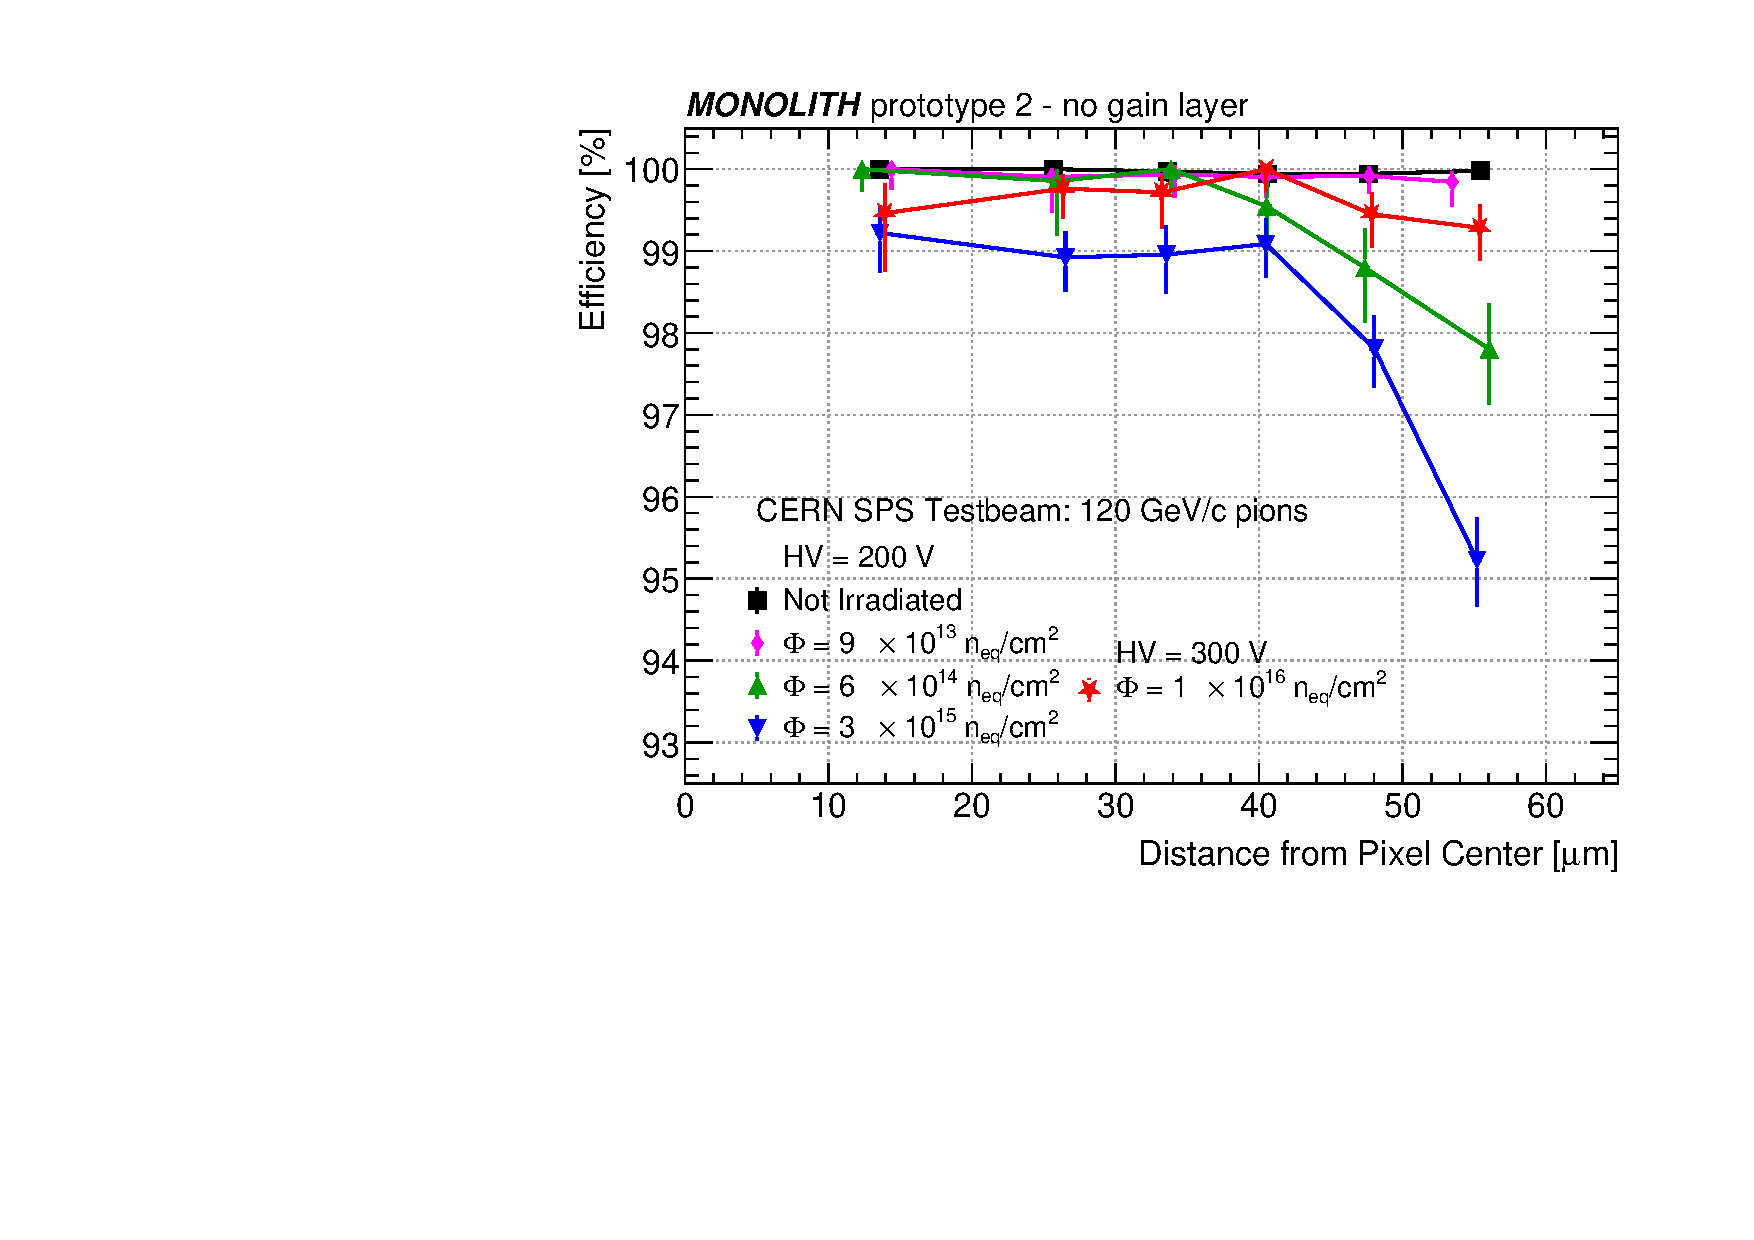
\includegraphics[width=.75\textwidth]{files/MONOLITH_Irradiated_paper/Radius_efficiency}
			\caption{Detection efficiency as a function of the distance from the pixel center. The data refer to power density \power~= 0.9 W/cm$^2$, voltage threshold  \vth~= 7 \noise and sensor bias voltage HV = 200 V, with the exception of the data taken at \maxflu, for which the sensor bias voltage was 300 V. The efficiency was computed in the following bins of distance from the pixel center in microns: $[0-21], [21-30], [30-37], [37-44], [44-51], [51-65]$. In each bin, the data points are plotted at the mean value of the track distance from the pixel center.}
			\label{im:MONO-IR_Eff_vs_distance}
		\end{figure}



		\subsection{Time resolution}
		The time resolution of the DUT was measured using as reference the timestamp of two precise MCP detectors that were located outside the FE-I4 telescope downstream the pion beam. 
		The sample of telescope tracks used for the measurement of the time resolution was the same used for the detection efficiency, with the only exception that all the tracks within the pixel were considered here, and not exclusively the tracks within the aforementioned triangle defined by the three analog pixel centres. 

		The ToA was measured for the DUT and the MCPs making offline a linear interpolation between the oscilloscope samplings and taking the time at which the signals reached 50\% of the maximum value of the signal amplitude.
		The difference in ToA between the three pairs of detectors was then used to extract the time resolution of the DUT, as explained in~\cite{Monolith_20ps}. 

		Taking the ToA at a fixed percentage of the signal amplitude has the advantage to correct for most of the time walk between signals with different amplitudes, under the assumption that signals of all amplitudes have consistent rise times. 
		It was observed that in our case this method carries the drawback of creating a small distortion of the distribution of the TOA difference, which deviates slightly from a Gaussian distribution and generates a tail at large values of ${\rm TOA}_{\it DUT}$ - ${\rm TOA}_{\it MCP}$.
		\begin{figure}[h]
			\centering 
			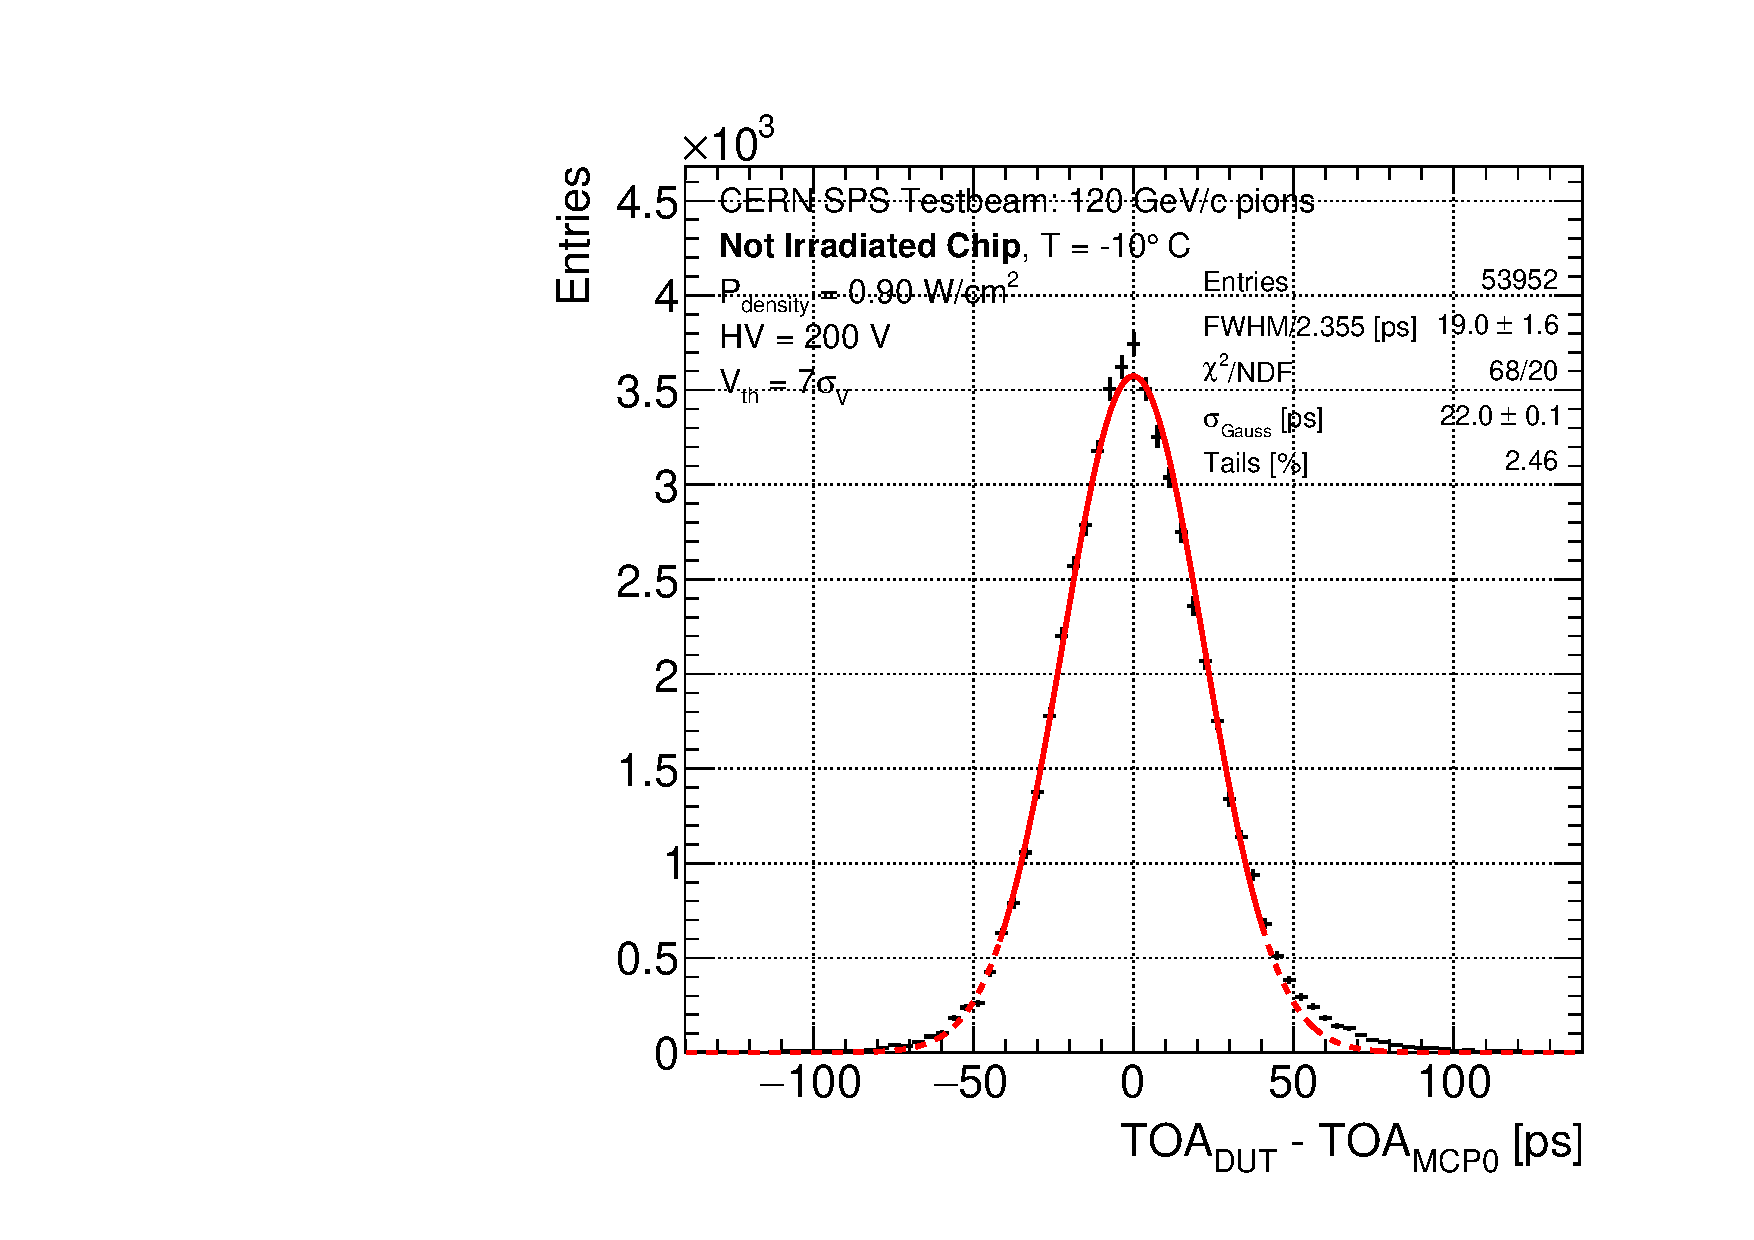
\includegraphics[width=.49\textwidth]{files/MONOLITH_Irradiated_paper/M06_fit20.pdf}
			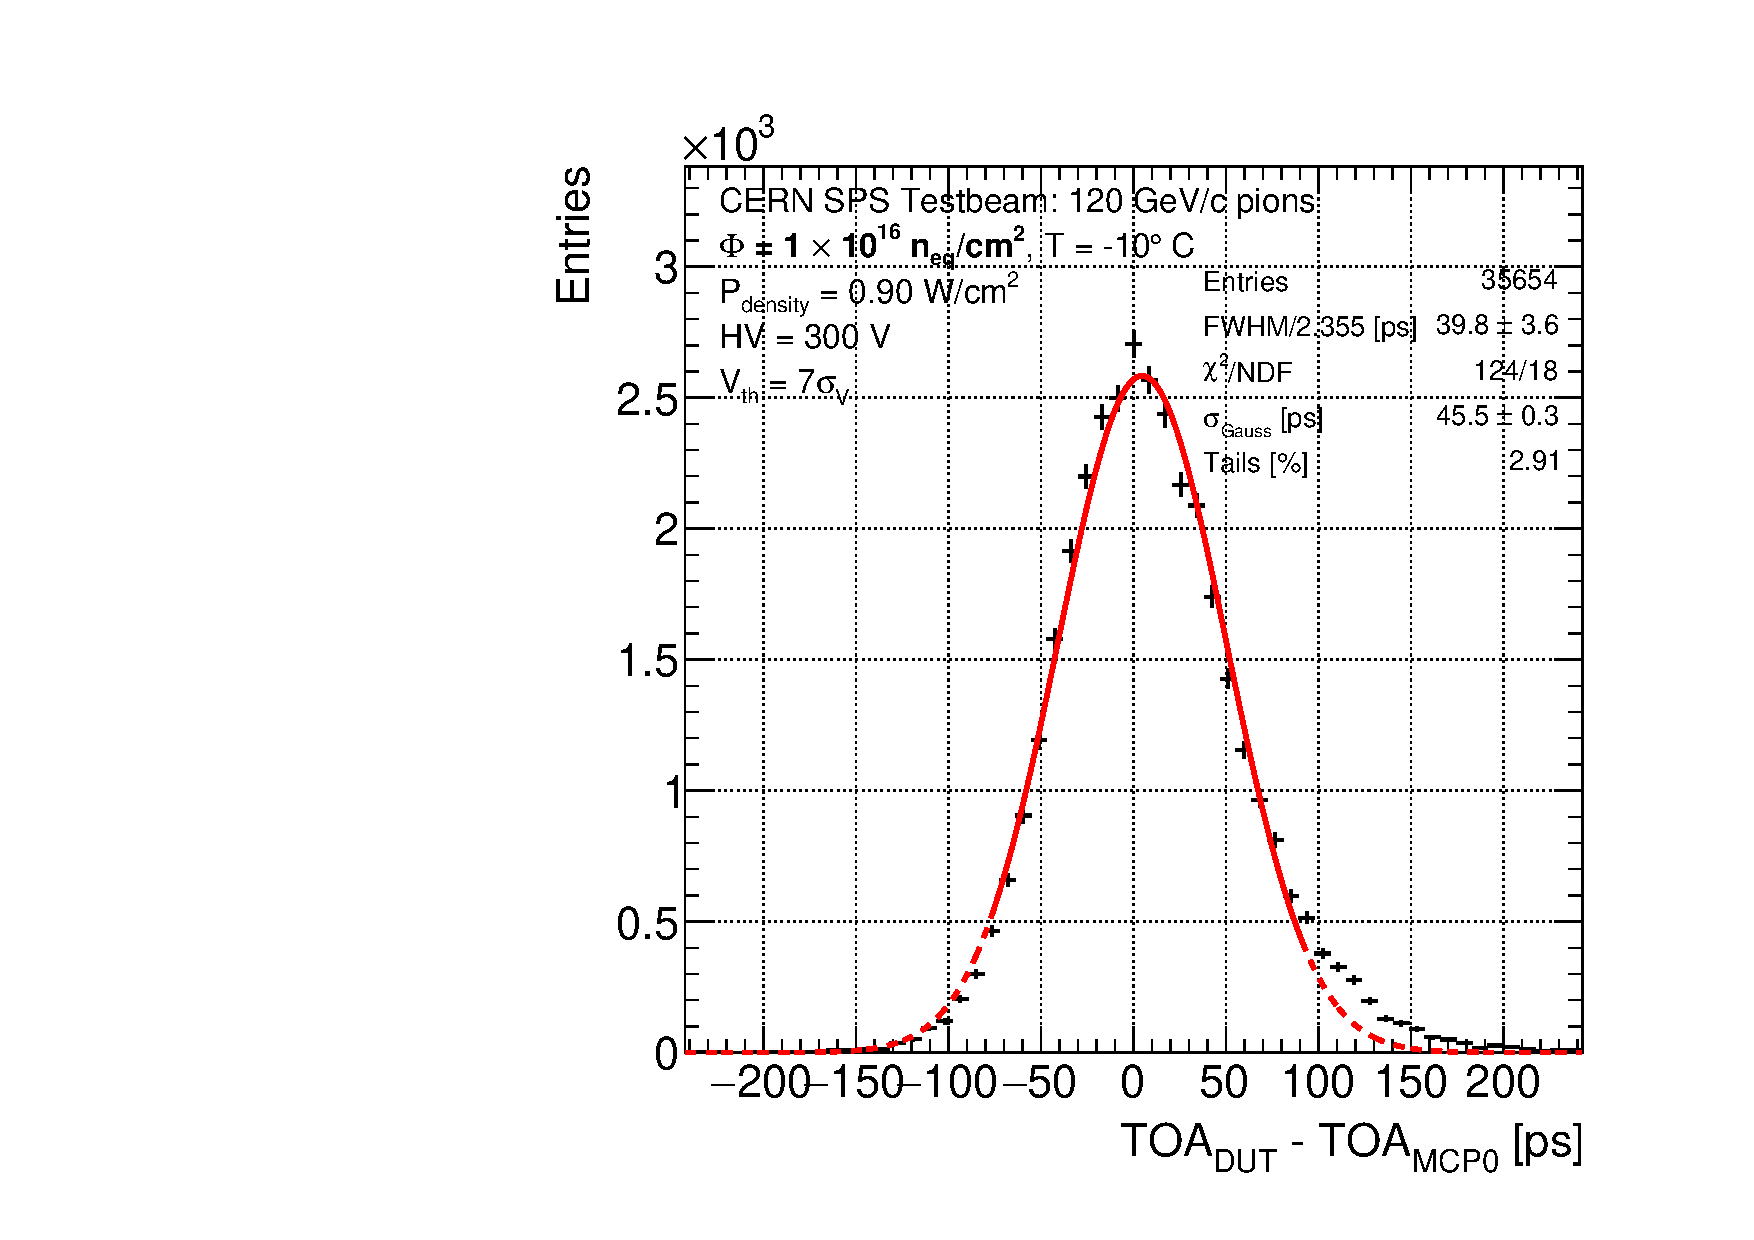
\includegraphics[width=.49\textwidth]{files/MONOLITH_Irradiated_paper/M16_300V_fit20.pdf}
			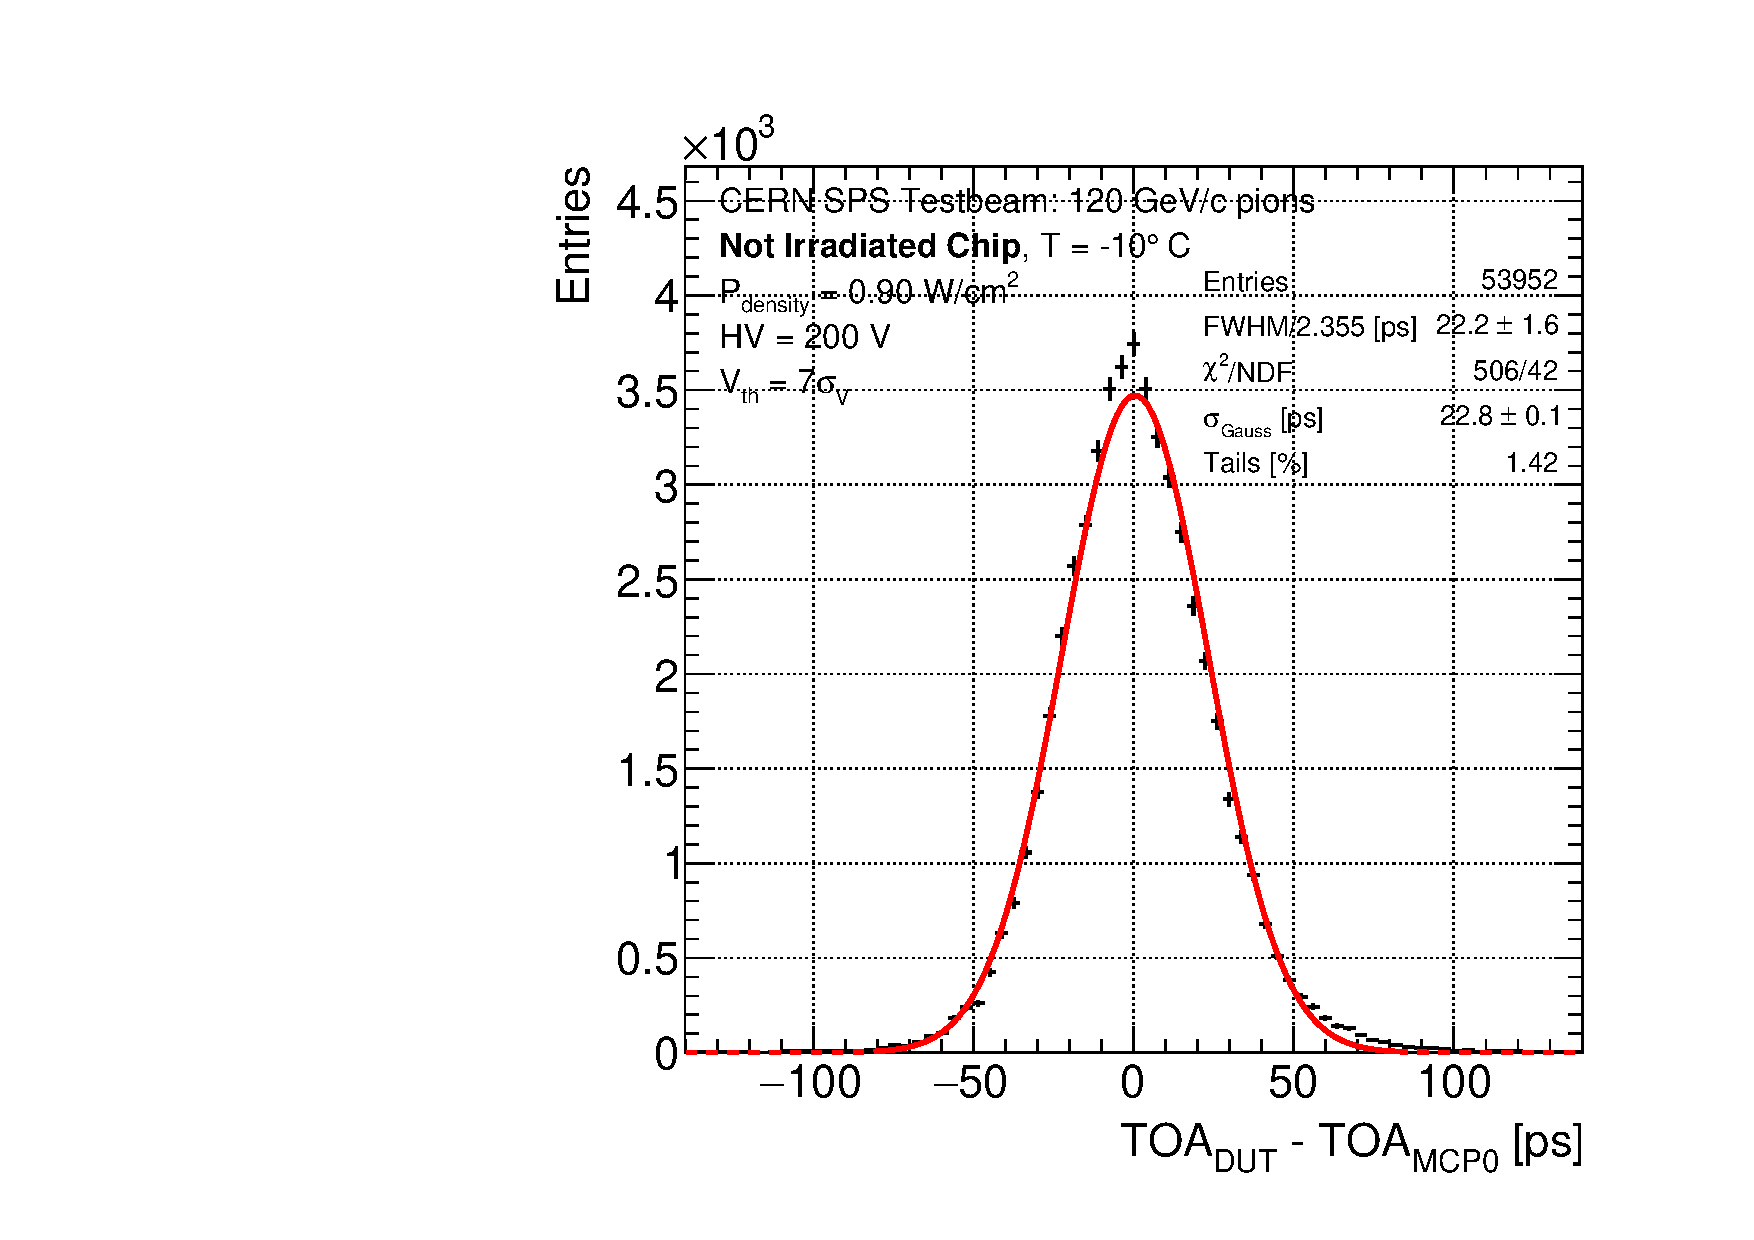
\includegraphics[width=.49\textwidth]{files/MONOLITH_Irradiated_paper/M06_fullfit.pdf}
			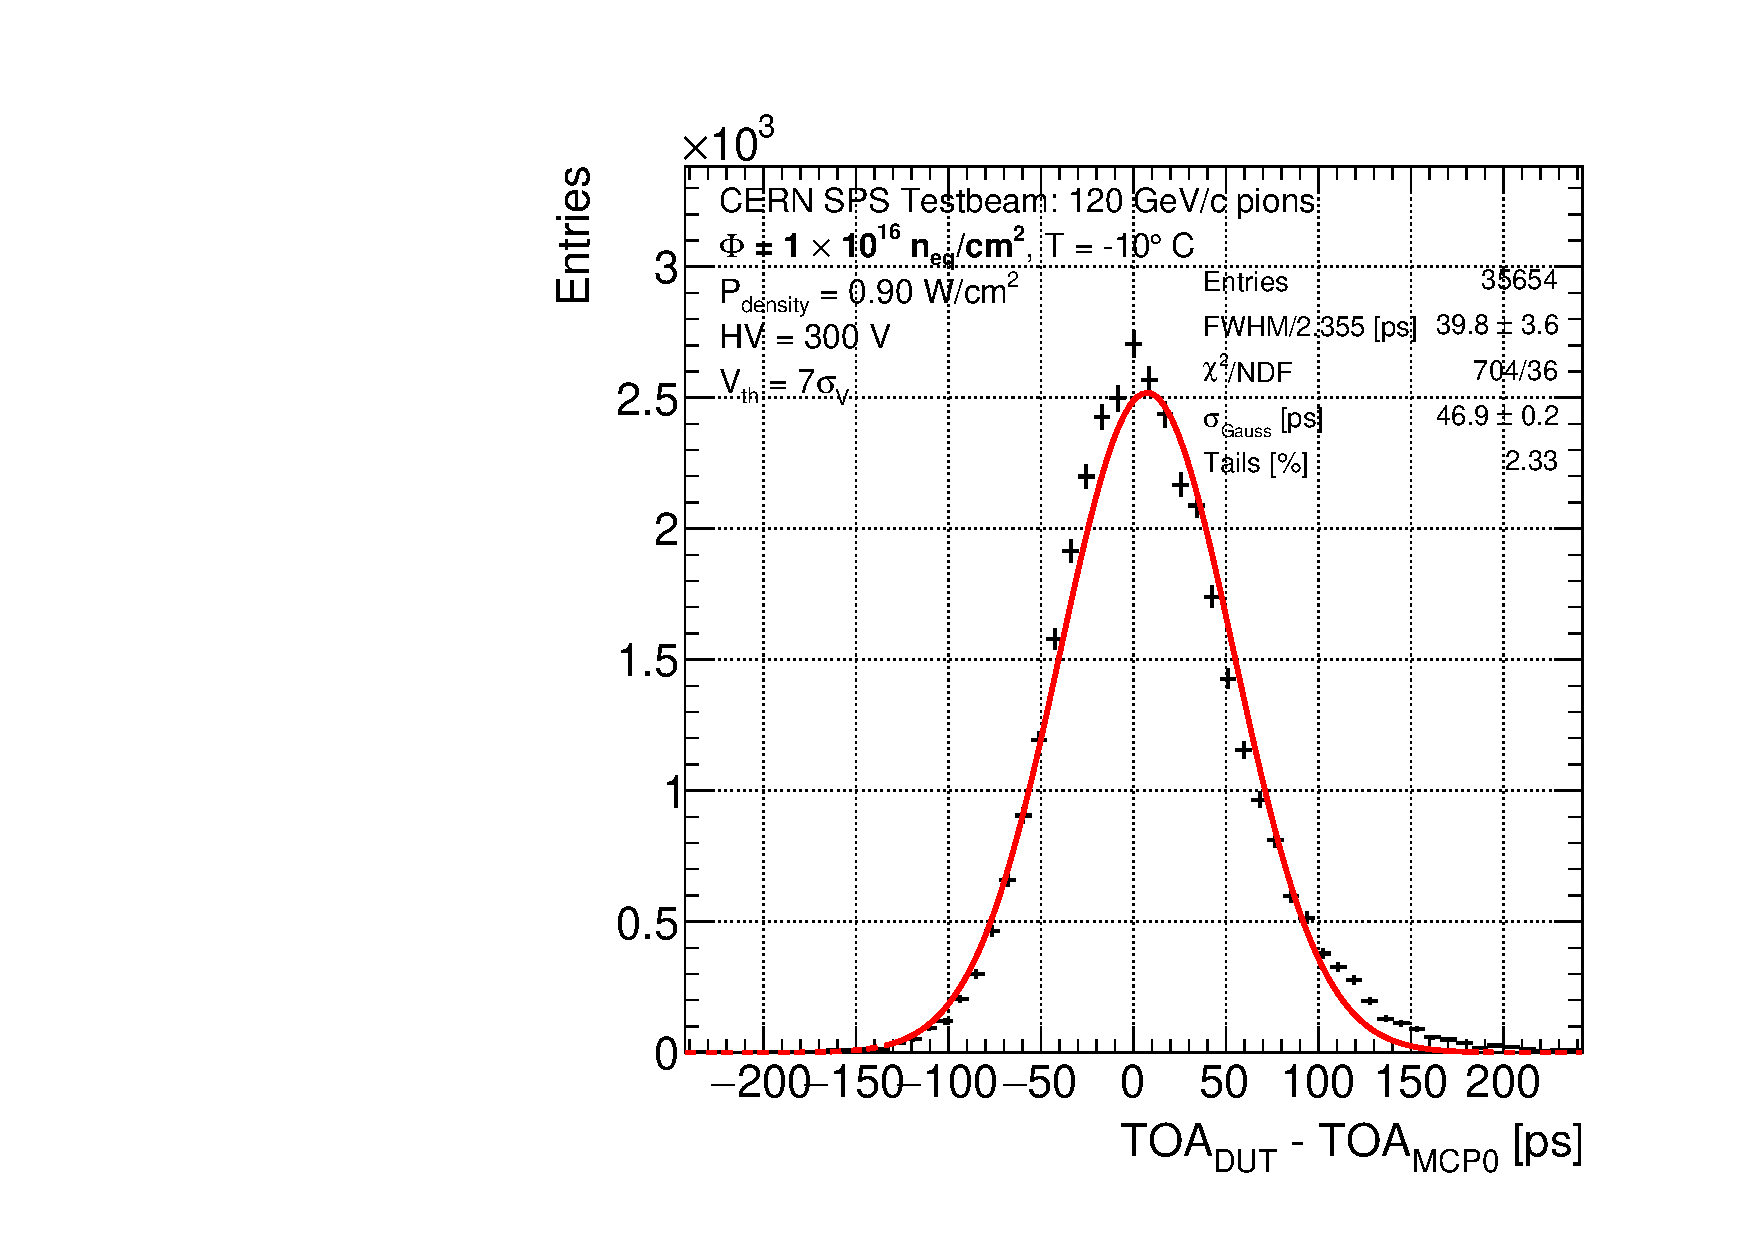
\includegraphics[width=.49\textwidth]{files/MONOLITH_Irradiated_paper/M16_300V_fullfit.pdf}
			\caption{Difference in ToA between the DUT and one of the MCP detectors used to provide a precise reference time. The left-hand panels show the results for the board not irradiated, while the right-hand panels those for the board irradiated to \maxflu. The top panels show the data with superimposed the Gaussian fits extending to the first bin containing 20\% of the maximum value of the distribution; the bottom panels show the same data with superimposed the Gaussian fits extending to all the bins of the distributions.}
			\label{im:MONO-IR_toa}
		\end{figure}
		This effect is shown in figure \ref{im:MONO-IR_toa} in the case of the board not irradiated (left panels) and of the board irradiated at \maxflu~(right panels). 

		To account for the observed distortion in the ToA difference, the $\sigma$ values from the Gaussian fits obtained using only the bins of the distribution larger than 20\% of the bin with the highest number of entries (two top panels in the figure \ref{im:MONO-IR_toa}) were used as central values of the time resolution.
		The difference between these values and those obtained by fitting a Gaussian functional form in the entire ToA-difference distributions (bottom panels in figure \ref{im:MONO-IR_toa}) were used as systematic uncertainty. These uncertainties were summed in quadrature with the statistical uncertainty coming from the Gaussian fits that were used as central values, and are shown as vertical error bars in the time resolution plots.

		\begin{figure}[h]
			\centering
			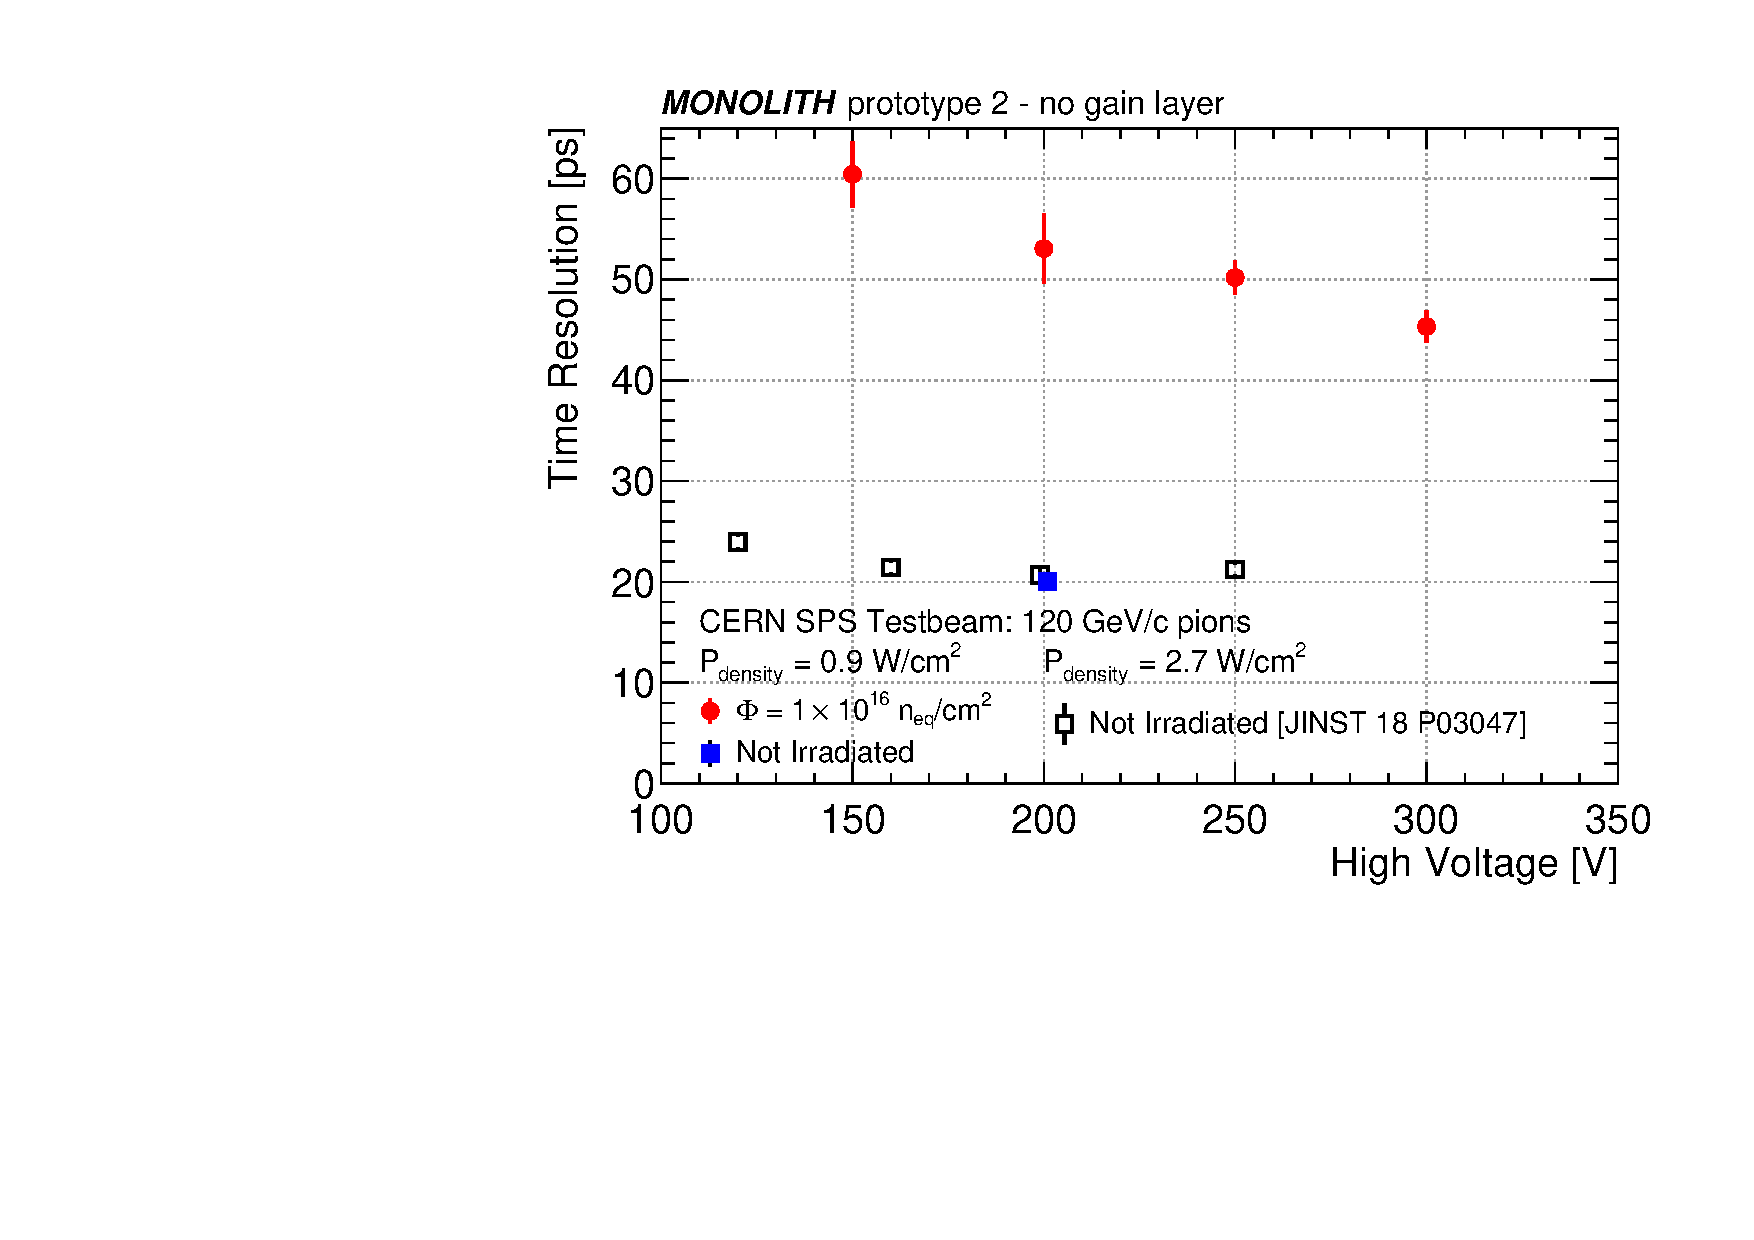
\includegraphics[width=.75\textwidth]{files/MONOLITH_Irradiated_paper/Voltage_timeresolution.pdf}
			\caption{Time resolution measured as a function of the sensor bias voltage. The results obtained with the board irradiated to \maxflu~at \power~= 0.9 W/cm$^2$ (red circles) are presented together with the result obtained with the board not irradiated at HV = 200 V (blue square). The plot results obtained in a previous testbeam~\cite{Monolith_20ps} with the board not irradiated at \power~= 2.7 W/cm$^2$ and  $i_{\it feedback}$ = 0.1 $\mu$A are also superimposed (black open squares).}
			\label{im:MONO-IR_HV_vs_timeres} 
		\end{figure}

		The last column of table \ref{tab:MONO-IR_effres} reports the time resolution obtained for the 18 datasets acquired at \vth~= 7 \noise.  

		Figure \ref{im:MONO-IR_HV_vs_timeres} shows the time resolution obtained at \power~= 0.9 W/cm$^2$ for the board irradiated to \maxflu~for a sensor bias voltage varying between 150 and 300 V, and the result obtained with the non-irradiated board at HV = 200 V. For comparison, the figure reports as well the time resolution measured at \power~= 2.7 W/cm$^2$ with the board not irradiated in previous testbeam experiment \cite{Monolith_20ps}.
		While the board not irradiated reaches the plateau of time resolution already at HV = 160 V, the time resolution measured with the irradiated board does not seem to have yet reached a plateau value at 300 V.

		\begin{figure}[h]
			\centering
			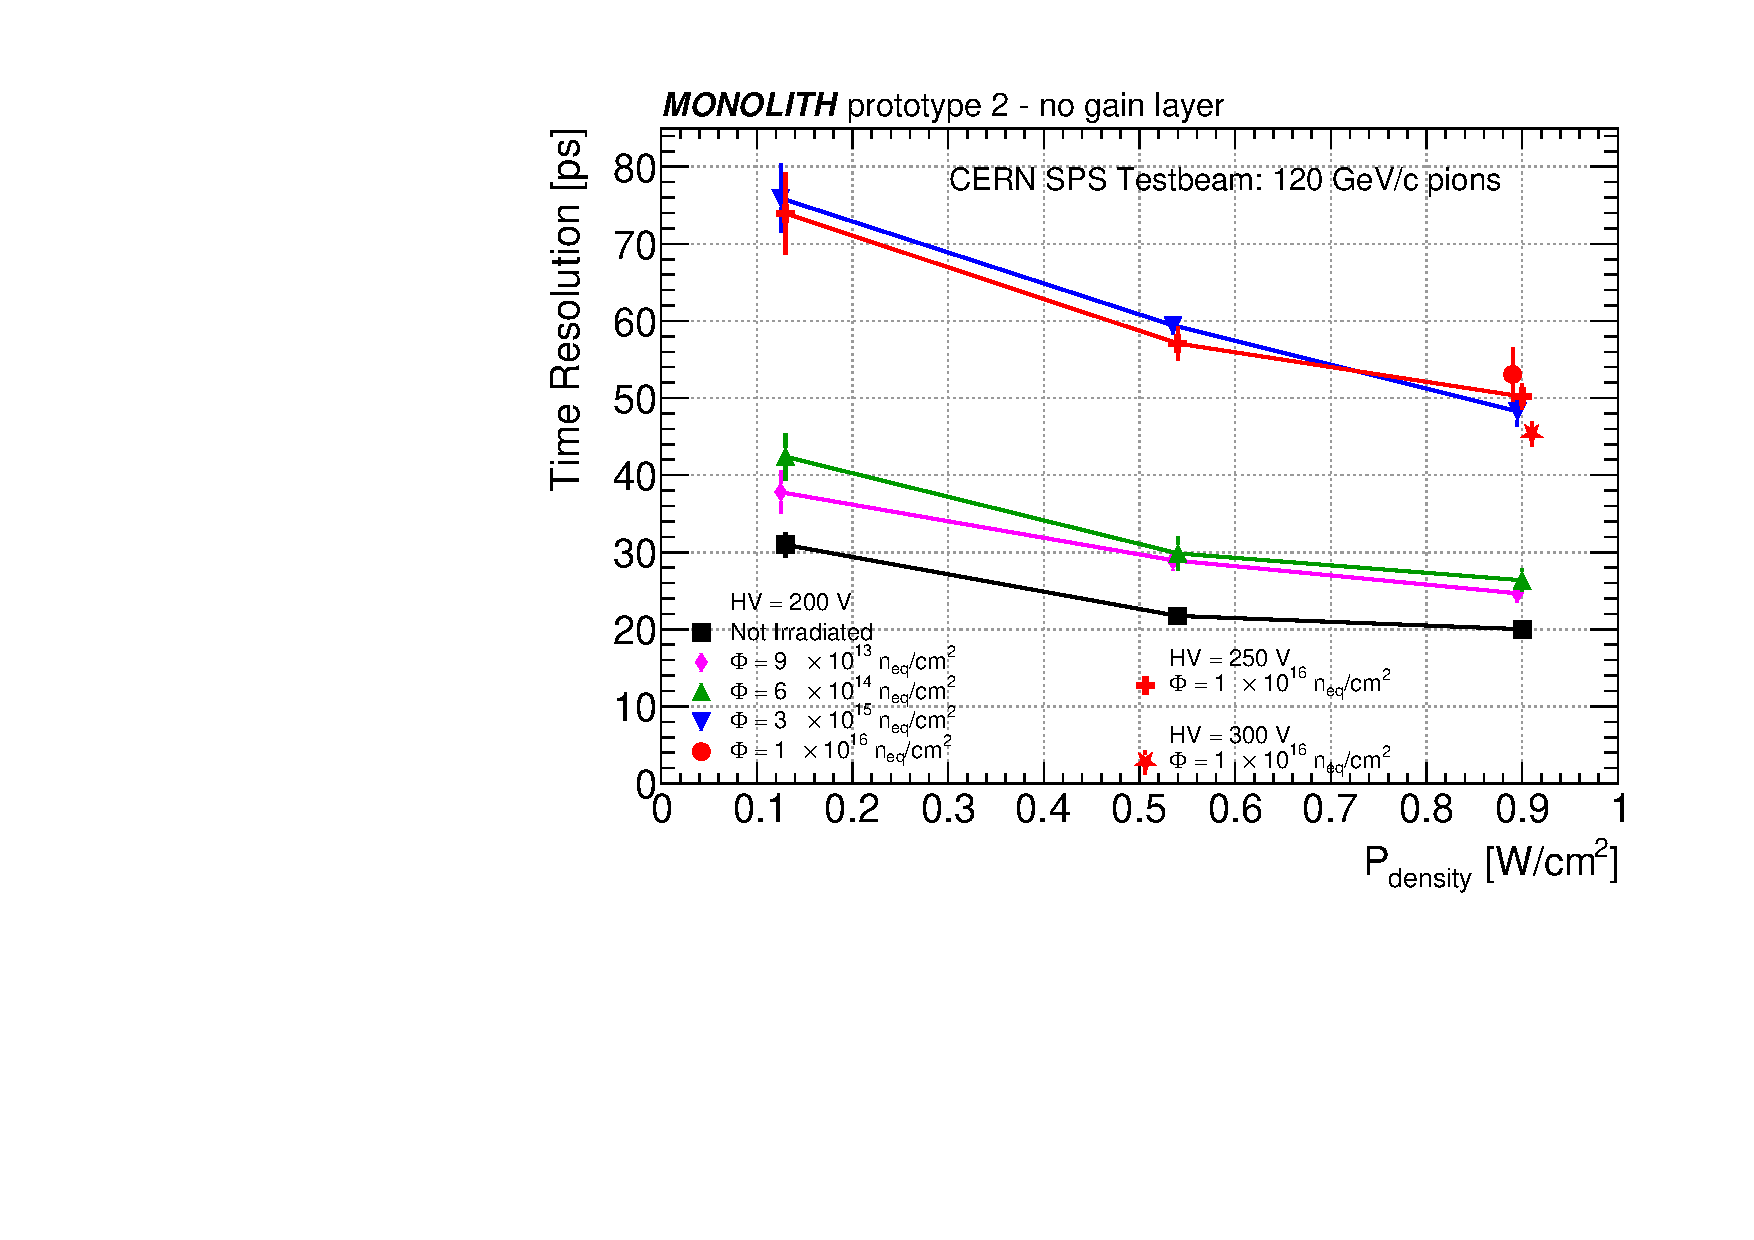
\includegraphics[width=.75\textwidth]{files/MONOLITH_Irradiated_paper/Power_timeresolution.pdf}
			\caption{Time resolution measured for three values of the  power density supplied to the preamplifier between 0.13 and 0.9 W/cm$^2$. The plot shows the results obtained at sensor bias voltage HV = 200 V with the five boards which were subject to proton fluence between zero and \maxflu. The data taken with the board most irradiated  at HV = 250 and 300 V are also shown.}
			\label{im:MONO-IR_power_vs_timeres}
		\end{figure}

		The time resolution of the DUT was also measured as a function of the power density supplied to the frontend electronics. The results are presented in figure \ref{im:MONO-IR_power_vs_timeres} at a sensor bias voltage HV = 200 V for all the boards, and for the most irradiated board also at HV = 250 and 300 V. In all cases, the time resolution was found to steadily improve with increasing \power, and degrade with increasing proton fluence. In the \power~range studied, it varies between 30 and 20 ps in the case of the board not irradiated, and between 75 and  50 ps in the case of the board irradiated to \maxflu.

		It should be noted that, for each of the irradiation values studied, the ratio of the time resolutions at \power~= 0.13 and 0.9 W/cm$^2$ is constant, showing a relative improvement of approximately 35\% independently of the fluence, as reported in table~\ref{tab:MONO-IR_Power_improvement}.  
 

		\begin{table}[h]
			\centering
			\renewcommand{\arraystretch}{1.2}
			\begin{tabular}{|c|c|c|c|}
			\cline{1-4}
			\multirow{2}{*}{\begin{tabular}{c}Fluence \\ \ [1 MeV n$_{\text{eq}}$/cm$^2$]\end{tabular} } & \multicolumn{2}{c|}{\begin{tabular}{c}  Time Resolution [ps] \end{tabular}} & \multirow{2}{*}{\begin{tabular}{c} Ratio  \end{tabular}} \\ \cline{2-3}
			&\power~ = 0.13 W/cm$^2$&\power~ = 0.9 W/cm$^2$& \\
			\cline{1-4}
			0                   & 31.0 $\pm$ 1.6 & 20.0 $\pm$ 1.0 & 1.55 $\pm$ 0.15 \\ \hline
			$9 \times 10^{13}$  & 37.8 $\pm$ 2.8 & 24.7 $\pm$ 1.0 & 1.53 $\pm$ 0.21 \\ \hline
			$6 \times 10^{14}$  & 42.4 $\pm$ 3.0 & 26.4 $\pm$ 1.5 & 1.61 $\pm$ 0.21 \\ \hline
			$3 \times 10^{15}$  & 75.9 $\pm$ 4.5 & 48.3 $\pm$ 1.9 & 1.57 $\pm$ 0.17 \\ \hline
			$1 \times 10^{16}$  & 74.0 $\pm$ 5.4 & 50.2 $\pm$ 1.6 & 1.57 $\pm$ 0.19 \\ \hline
			\end{tabular}
			\caption{Time resolution measured with the five boards at \power~= 0.13 and 0.9 W/cm$^2$ and their ratio. The data were taken at sensor bias voltage HV = 200 V for all boards except the board irradiated to \maxflu~for which the sensor bias voltage was 250 V.}
			\label{tab:MONO-IR_Power_improvement} 
		\end{table}


		This is an indication that the dependence of the transition frequency from the collector current, which is observed in \cite{SiGeRadiationDamage} not to change up to 1 $\times$ 10$^{14}$ \flu, might not be affected by radiation damage even at \maxflu. 

		\begin{figure}[h]
			\centering
			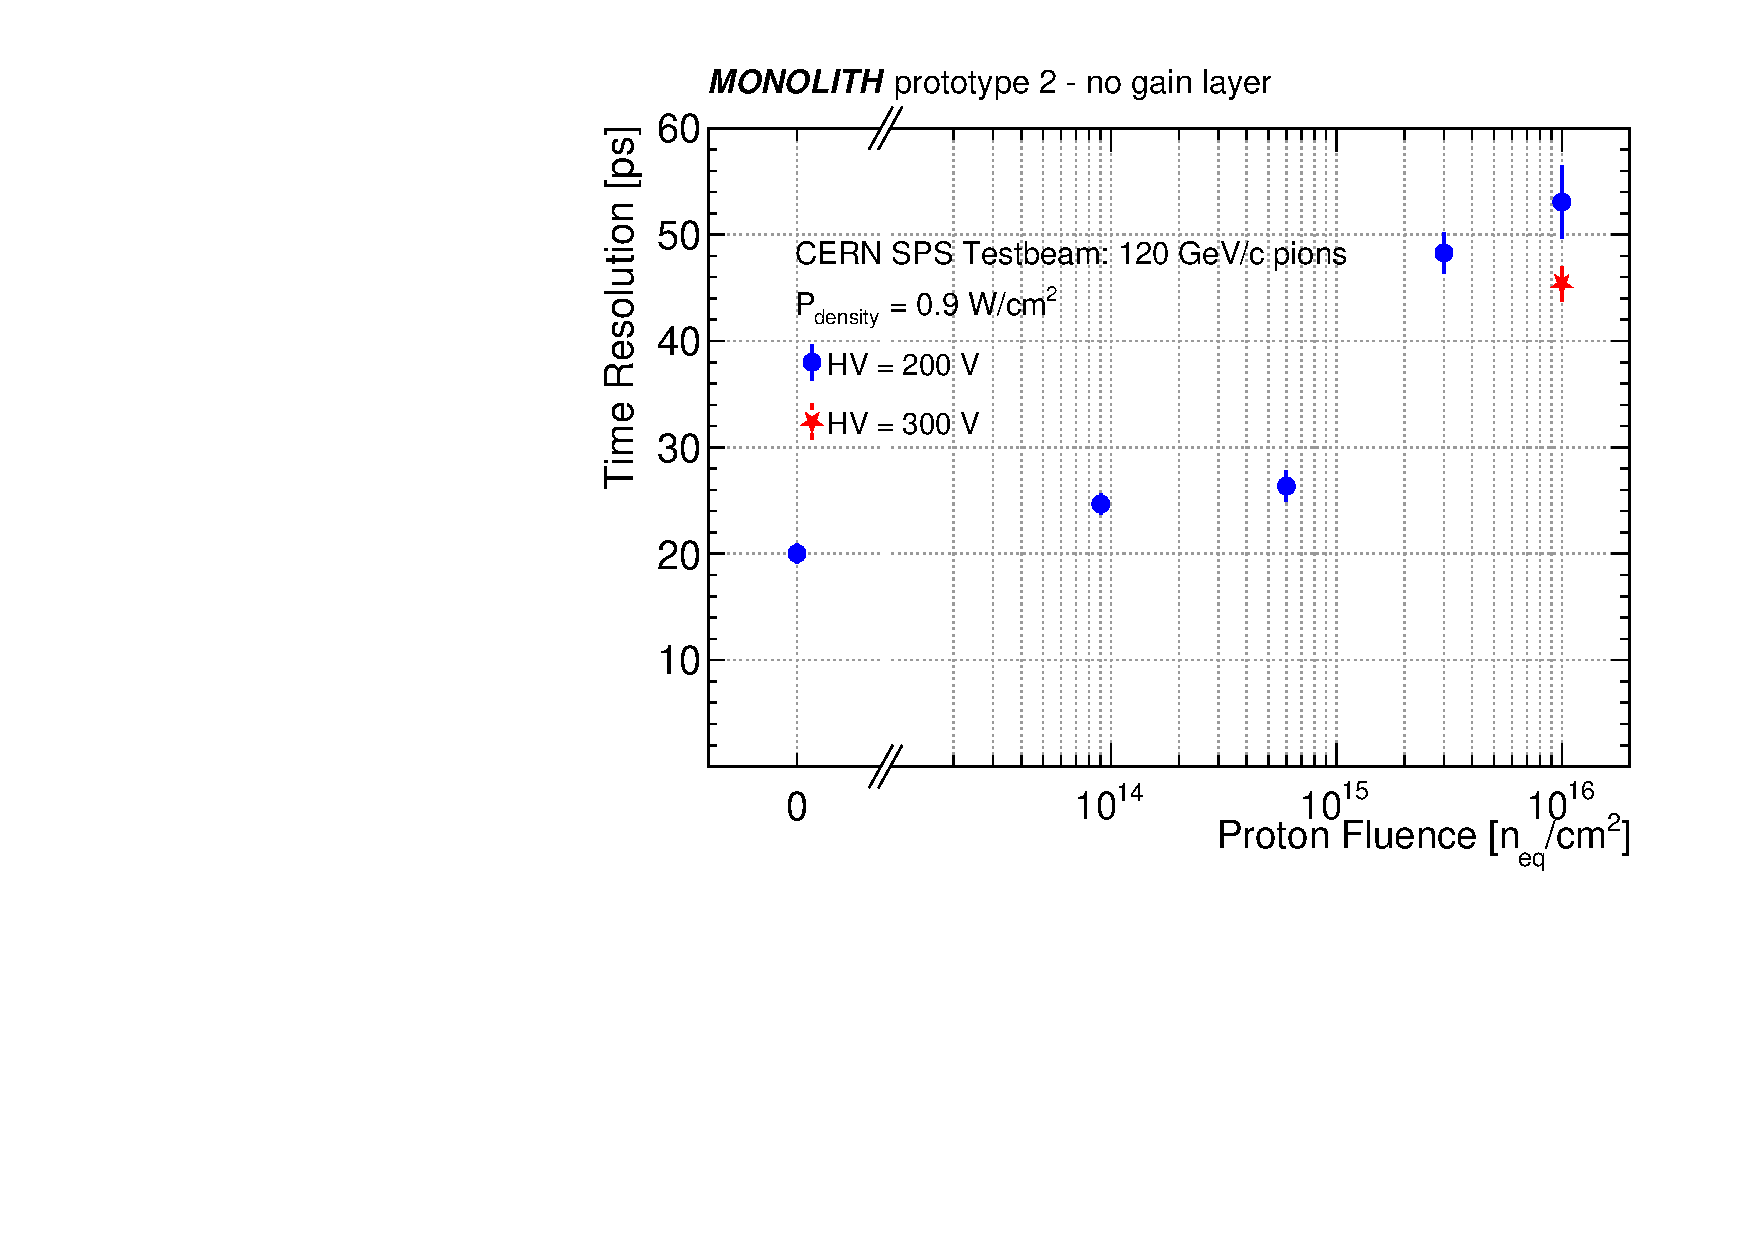
\includegraphics[width=.67\textwidth]{files/MONOLITH_Irradiated_paper/Fluence_log_timeresolution.pdf}
			\caption{Time resolution as a function of the proton fluence for \power~= 0.9 W/cm$^2$. The blue dots show the results obtained at a sensor bias voltage HV = 200 V, while the red star shows the result obtained at HV = 300 V with the board irradiated to \maxflu.}
			\label{im:MONO-IR_fluence_vs_timeres} 
		\end{figure}

		Figure \ref{im:MONO-IR_fluence_vs_timeres} shows the time resolutions as a function of the proton fluence at \power~= 0.9 W/cm$^2$. The results obtained with the datasets taken at sensor bias voltage HV = 200 V vary between 20 ps for the board not irradiated and 53 ps for the board irradiated to \maxflu. 
		For this last board, an increase of the sensor bias voltage to 300 V provides a time resolution of 45 ps, thus improving it by approximately 10\%.

		\begin{figure}[!htb]
			\centering
			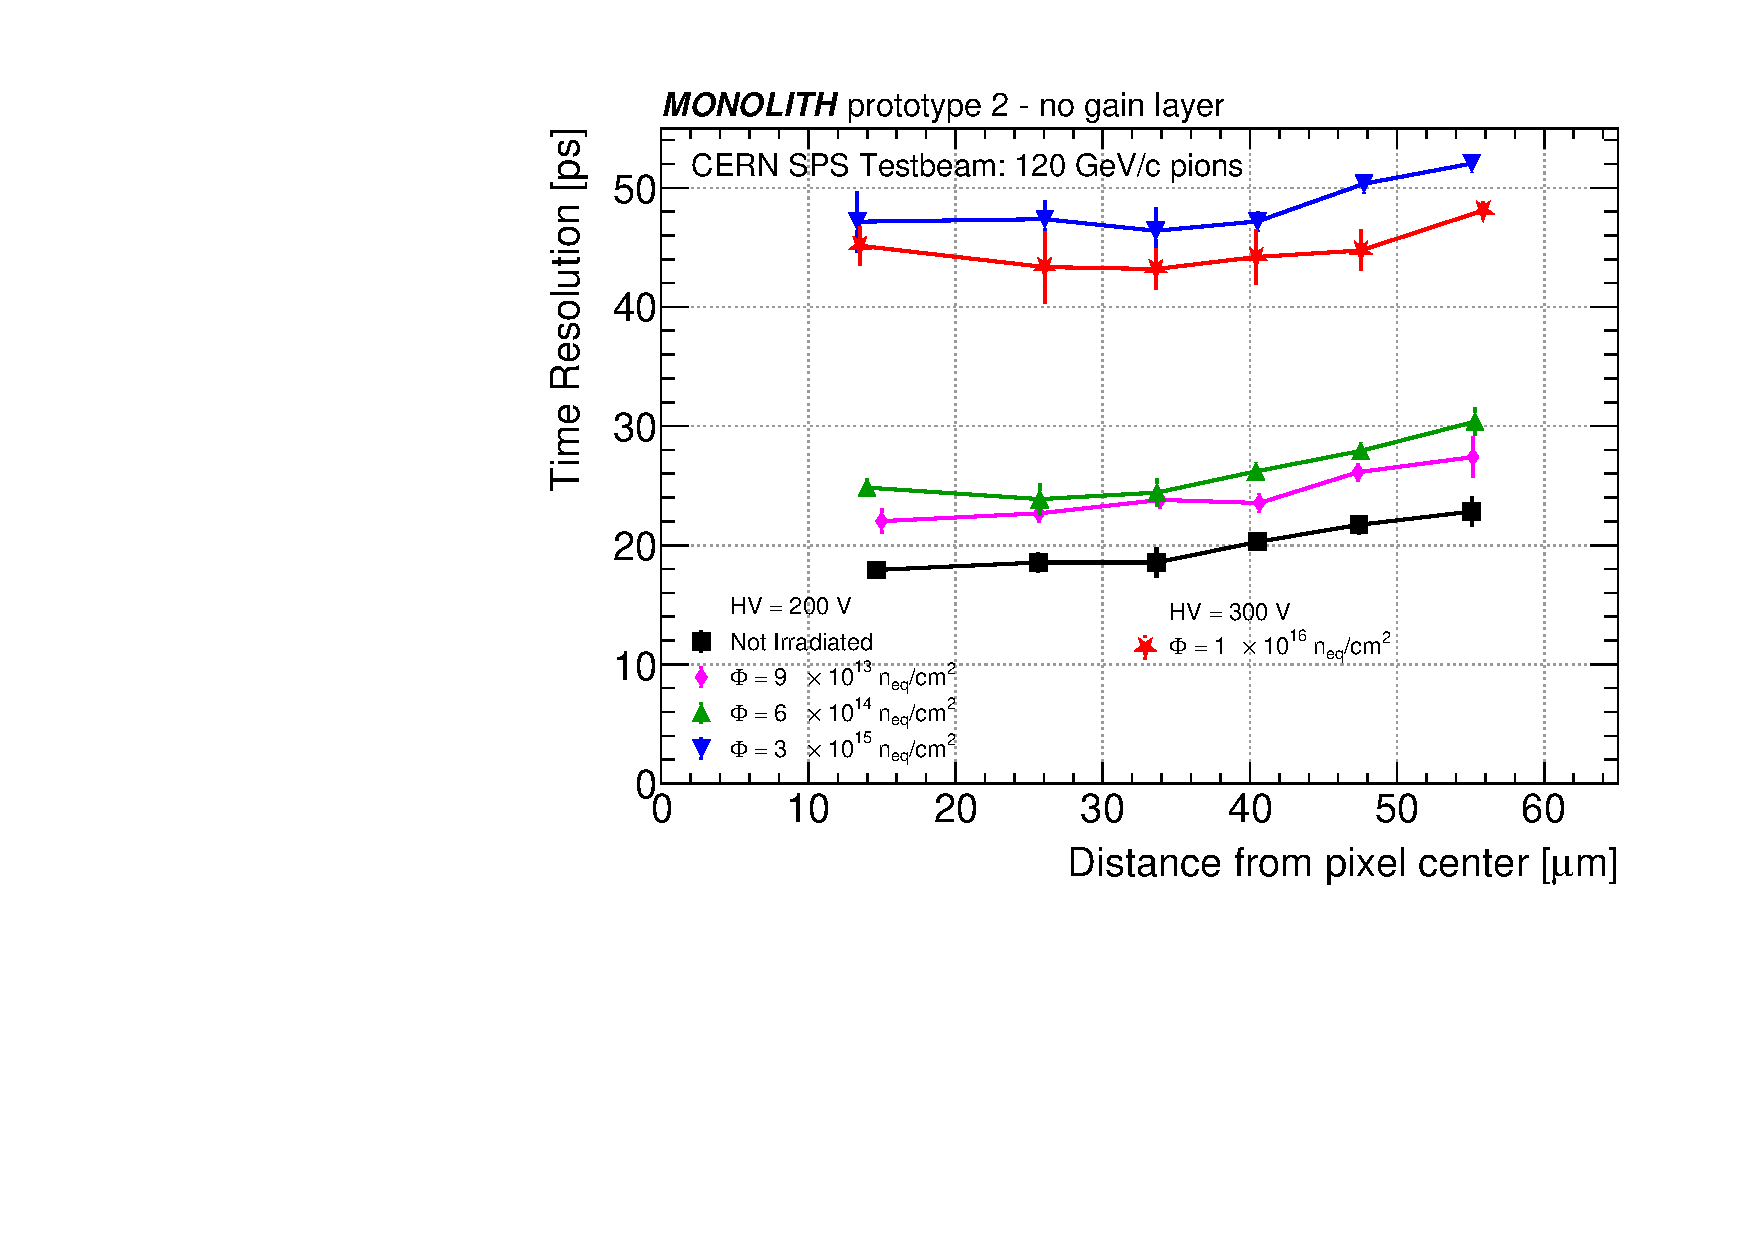
\includegraphics[width=.67\textwidth]{files/MONOLITH_Irradiated_paper/Radius_timeresolution}
			\caption{Time resolution as a function of the distance from the pixel center. The data refer to \power~= 0.9 W/cm$^2$,  \vth~= 7 \noise~and HV = 200 V, with the exception of the data taken at \maxflu, for which the sensor bias voltage was 300 V. The time resolution was computed in the same bins of figure \ref{im:MONO-IR_Eff_vs_distance}.}
			\label{im:MONO-IR_Timeres_vs_distance}
		\end{figure}

		The time resolution is shown as a function of the distance from the centre of the pixel in figure \ref{im:MONO-IR_Timeres_vs_distance}.
		All the data refer to a sensor bias voltage of 200 V, with the exception of the dataset at \maxflu, which was acquired at 300 V.
		For all fluences the time resolution is better in the central region of the pixel than in the inter-pixel region, where it increases approximately 5 ps.
		